\chapter[Auswertung der Onlinebefragung zur Kasusrektion]{Auswertung der Onlinebefragung zur Kasusrektion von \object{wegen}, \object{während}, \object{dank}, \object{gegenüber} und \object{seit}}
\label{cha:Ergebnisse}
Im folgenden Kapitel werden die Ergebnisse aus der Onlinebefragung zum Zusammenhang zwischen Metapragmatik und Sprachgebrauch der Rektionskasus von \wegen, \waehrend, \dank{} und \gegenueber{} sowie der Primärpräposition \object{seit} präsentiert. 
Die Analyse richtet sich dabei nicht nach der Reihenfolge der Erhebung der Daten im Fragebogen, sondern leitet sich aus dem Forschungsinteresse ab und ermöglicht eine schrittweise Datenanalyse:
Einleitend wird ein Überblick über die Zusammensetzung der Gruppe der Befragten gegeben (\autoref{sec:Befragte}).
Dabei werden auch die allgemeinen Ansichten über Sprache thematisiert, die die Befragten im Fragebogen äußern. 
\autoref{sec:ErgAss} widmet sich den freien Assoziationen, die Befragte mit den Rektionsvarianten haben, sowie den semantischen Differenzialen. 
Vor dem Hintergrund der Ergebnisse der Assoziationsstudie werden anschließend die Angaben im Akzeptabilitätstest (\autoref{sec:ErgAkz}) sowie die Kasuswahl im Produktionsexperiment (\autoref{sec:ErgProduktion}) ausgewertet und interpretiert. % Änderung Anfang
Sowohl für die Akzeptabilität als auch für die Produktion wird mithilfe statistischer Modelle (\textit{random forests}) die Relevanz der unterschiedlichen Einflussfaktoren überprüft.%Änderung Ende
%Schließlich wirft \autoref{sec:ErgPositionierung} einen Blick darauf, wie sich einzelne ausgewählte Befragte im Verlauf des Fragebogens zu den Rektionsvarianten positionieren. 
\section{Zusammensetzung der Befragtengruppe}
\label{sec:Befragte}
An der Befragung nahmen 397 Personen teil, die angaben, deutsche MuttersprachlerInnen zu sein und in Deutschland zu leben. 
Im Folgenden wird vorgestellt, wie sich die Gruppe bezüglich soziodemografischer Merkmale sowie hinsichtlich der Angaben zu Sprachbewusstheit, Sprachsicherheit und Variationstoleranz zusammensetzt. 
Dabei geht es zunächst um Alter und Gender der Befragten (\autoref{sec:AlterundGender}), dann um ihre regionale Herkunft und die Dialektkompetenz (\autoref{sec:HerkunftundDialekt}), ihren Bildungsstand (\autoref{sec:Bildung}) und anschließend darum, wie häufig Befragte in ihrem Beruf mit längeren Texten zu tun haben (\autoref{sec:Beruf}). 
\autoref{sec:Sprachbewusstheit} bis \autoref{sec:Variationstoleranz} thematisieren die Angaben der Befragten auf den Likertskalen zu Sprachbewusstheit, Sprachsicherheit und Variationstoleranz.  
\subsection{Alter und Gender der Befragten}
\label{sec:AlterundGender}
234 Befragte gaben an, weiblichen Geschlechts zu sein, 155 gaben an, männlichen Geschlechts zu sein und eine Person gab an, ein anderes Geschlecht zu haben (s. \autoref{table:GenderAnh} im Anhang). 
Sieben Personen machten keine Angabe zu ihrem Geschlecht. 
Der Anteil weiblicher Befragter überwiegt demnach mit 59~\%. 39~\% der Befragten sind männlich. 

Die Befragten sind zwischen 18 und 85 Jahre alt. 
Das Durchschnittsalter liegt bei 37, die Standardabweichung bei 16,2. 
Für die Auswertung werden folgende vier Altersgruppen zusammengefasst: 18--25, 26--35, 36--60 und 61--85 (s. \autoref{table:AltersgruppenAnh} im Anhang).
Der Anteil junger TeilnehmerInnen überwiegt: Über 60~\% der Befragten sind unter 36 Jahre alt.
Aus diesem Grund wurden bei den ersten beiden Altersguppen kleinere Spannen angelegt als bei den beiden letzteren. 
Insgesamt gehören 104 Befragte (ca. 26~\%) der jüngsten Altersgruppe an und 144 (ca. 36~\%) der Gruppe der 26- bis 35-Jährigen.
Nur etwas über 30~\% der Befragten sind 36 Jahre oder älter:
82 Personen (ca. 21~\%) sind 36 bis 60 Jahre alt und 47 Befragte (knapp 12~\%) finden sich in der Gruppe der über 60-Jährigen. 
Ungefähr 5~\% der BefragungsteilnehmerInnen machen keine Altersangabe.

\autoref{pic:AlterundGender} zeigt, wie sich Gender und Alter zueinander verhalten. 
In allen Altersgruppen überwiegt der Anteil weiblicher Befragter, in der Gruppe der 18- bis 25-Jährigen sind prozentual jedoch besonders viele weibliche Befragte vertreten. 
Hier ist das Verhältnis von weiblichen zu männlichen Befragten 68 zu 30~\%. 

\begin{figure}
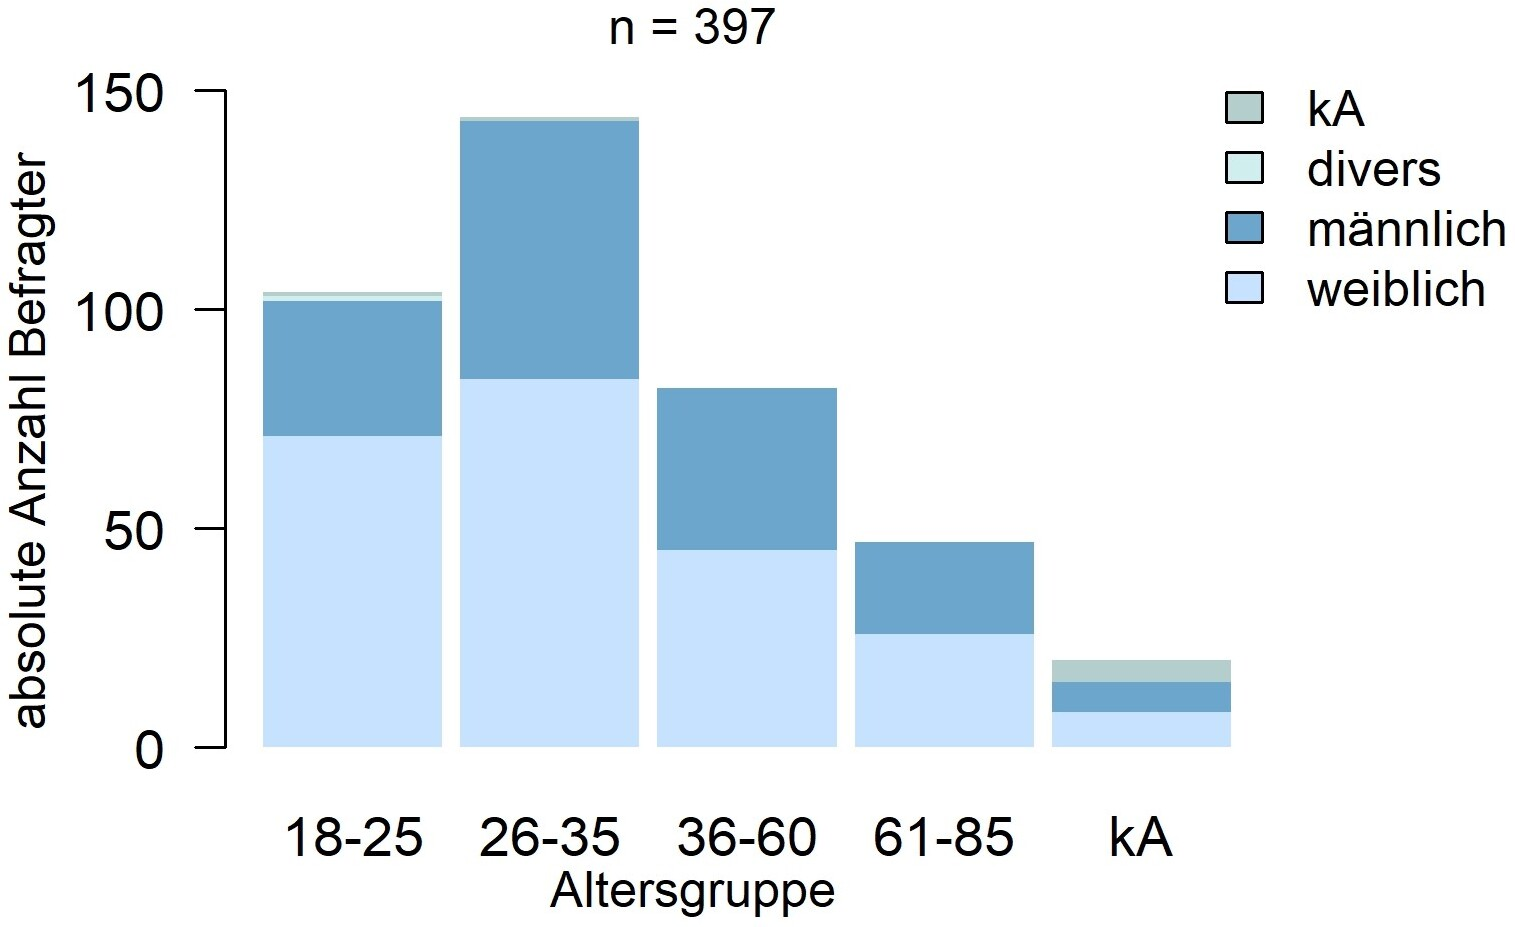
\includegraphics[width=\textwidth]{AlterundGender.jpg}
\caption{Genderzusammensetzung der Altersgruppen}
\label{pic:AlterundGender}
\end{figure}
%\begin{table}
%\centering
%\begin{tabular}{lrrrrrrrrr}
%\textbf{}             & \multicolumn{2}{l}{weiblich} & \multicolumn{2}{l}{männlich} & \multicolumn{2}{l}{divers} & \multicolumn{2}{l}{kA} & \multicolumn{1}{l}{gesamt} \\ \hline
%\textbf{18-25 Jahre}  & 71         & (68 \%)         & 31         & (30 \%)         & 1         & (1 \%)         & 1            & (1 \%)            & 104                        \\ \hline
%\textbf{26-35 Jahre}  & 84         & (58 \%)         & 59         & (41 \%)         & 0         & (0 \%)         & 1            & (1 \%)            & 144                        \\ \hline
%\textbf{36-60 Jahre}  & 45         & (55 \%)         & 37         & (45 \%)         & 0         & (0 \%)         & 0            & (0 \%)            & 82                         \\ \hline
%\textbf{61-85 Jahre}  & 26         & (55 \%)         & 21         & (45 \%)         & 0         & (0 \%)         & 0            & (0 \%)            & 47                         \\ \hline
%\textbf{kA} & 8          & (40 \%)         & 7          & (35 \%)         & 0         & (0 \%)         & 5            & (25 \%)           & 20                         \\ \hline
%\end{tabular}
%\caption{Genderzusammensetzung der Altersgruppen}
%\label{table:AlterundGender}
%\end{table}

\subsection{Regionale Herkunft und Dialektkompetenz der Befragten}
\label{sec:HerkunftundDialekt}
Die Befragten sind regional über ganz Deutschland verteilt, wenn auch ungleichmäßig (für die genauen Zahlen s. \autoref{table:HerkunftAnh} im Anhang): 
Ca. 43~\% der Befragten kommen aus norddeutschen Bundesländern, zu denen Schleswig-Holstein, Niedersachsen, Bremen und Hamburg gerechnet werden. 
% Änderung Anfang
Jeweils ca. ein Viertel der TeilnehmerInnen stammt aus südlichen (Bayern und Baden-Württemberg) oder westlichen bzw. südwestlichen (Nordrhein-Westfalen, Hessen, Rheinland-Pfalz und Saarland) Bundesländern und nur 6,5~\% kommen aus einem östlichen oder nordöstlichen Bundesland (Brandenburg, Mecklenburg-Vorpommern, Sachsen, Thüringen, Sachsen-Anhalt, Berlin).\footnote{Diese Einteilung wurde so vorgenommen, da das Ungleichgewicht zwischen den Befragtengruppen Nord oder Süd und den Gruppen Ost bzw. West bspw. bei Zuordnung von Mecklenburg-Vorpommern zu Norddeutschland vermutlich noch stärker gewesen wäre.
Ein zweiter Grund war die Vergleichbarkeit zwischen der Befragtengruppe aus dem Norden und derjenigen aus dem Süden (s. \autoref{sec:ErgAkzNachRegion} und \autoref{sec:ErgProdNachHerkunft}, vgl. auch \autoref{sec:ME}).}
% Änderung Ende

Betrachtet man die regionale Herkunft nach dem Alter der Befragten, fällt auf, dass die Verteilung nicht in allen Altersgruppen gleich ist (s. \autoref{pic:AlterundHerkunft}). 
In der Gruppe der über 60-Jährigen stammen mit 79~\% deutlich mehr Personen aus norddeutschen Bundesländern als in den anderen Altersgruppen. 
Unter den 18- bis 25-Jährigen ist dagegen der Anteil der Befragten aus Süddeutschland erhöht. 
Andersherum heißt dies auch, dass unter den norddeutschen Befragten besonders viele ältere Personen sind, während sich unter den süddeutschen Befragten besonders viele jüngere Personen finden. 
Dies lässt sich dadurch erklären, dass die Nacherhebung, bei der gezielt ältere Personen gewonnen werden sollten, insbesondere über den Mailverteiler eines norddeutschen Seniorenchors erfolgte (\autoref{sec:VerbreitungFragebogen}). 
Das Ungleichgewicht muss bei späteren Vergleichen nach Alter oder Herkunft der Befragten berücksichtigt werden. 
\begin{figure}
\centering
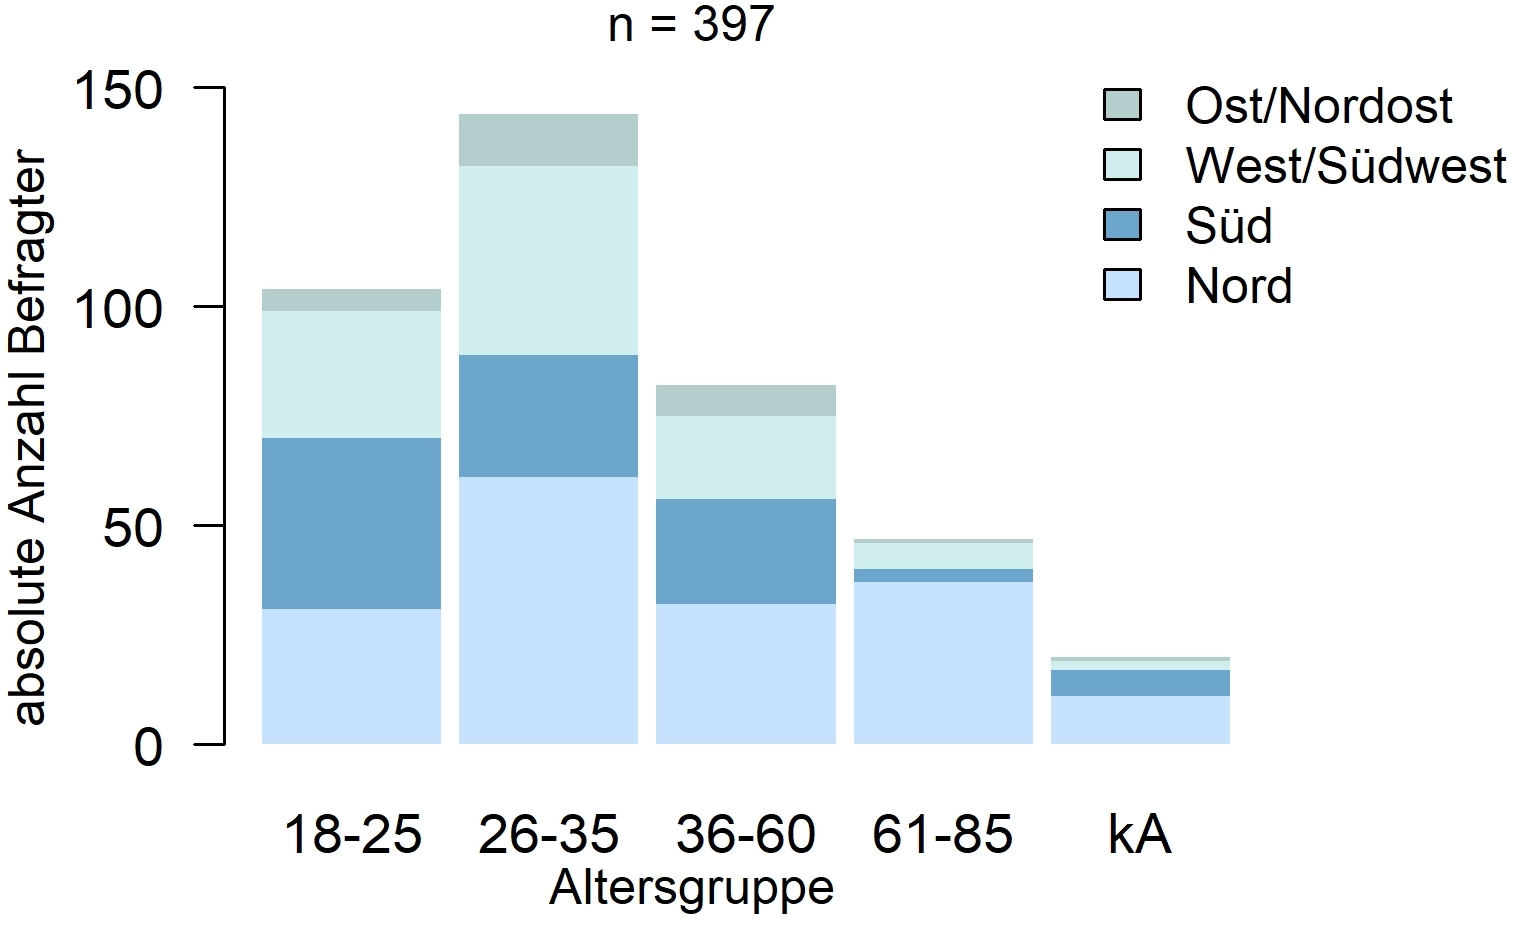
\includegraphics[width=\textwidth]{AlterundHerkunft.jpg}
\caption{Regionale Herkunft in den einzelnen Altersgruppen}
\label{pic:AlterundHerkunft}
\end{figure}
%\begin{table}
%\centering
%\begin{tabular}{lrrrrrrrrr}
%\textbf{}             & \multicolumn{2}{l}{Nord} & \multicolumn{2}{l}{Süd} & \multicolumn{2}{l}{Ost} & \multicolumn{2}{l}{West} & gesamt \\ \hline
%\textbf{18-25 Jahre}  & 31       & (30 \%)       & 39       & (38 \%)      & 5        & (5 \%)       & 29       & (28 \%)       & 104    \\ \hline
%\textbf{26-35 Jahre}  & 61       & (42 \%)       & 28       & (19 \%)      & 12       & (8 \%)       & 43       & (30 \%)       & 144    \\ \hline
%\textbf{36-60 Jahre}  & 32       & (39 \%)       & 24       & (29 \%)      & 7        & (9 \%)       & 19       & (23 \%)       & 82     \\ \hline
%\textbf{61-85 Jahre}  & 37       & (79 \%)       & 3        & (6 \%)       & 1        & (2 \%)       & 6        & (13 \%)       & 47     \\ \hline
%\textbf{keine Angabe} & 11       & (55 \%)       & 6        & (30 \%)      & 1        & (5 \%)       & 2        & (10 \%)       & 20     \\ \hline
%\end{tabular}
%\caption{Regionale Herkunft in den einzelnen Altersgruppen}
%\label{table:AlterundHerkunft}
%\end{table}

In einer offenen Frage wurde nach der Dialektkompetenz der TeilnehmerInnen gefragt. 
Von allen Befragten geben 160 (40~\%) an, dass sie in ihrer Familie, mit Freunden oder in anderen Situationen einen Dialekt sprechen. 
Da eine freie Angabe des Dialekts möglich war, fallen die Antworten sehr unterschiedlich aus: 
Genannt werden teils spezifische Dialekte wie Moselfränkisch, teils Regionalsprachen wie Norddeutsch.  
Einige Antworten enthalten außerdem Angaben zur Intensität des Dialekts (\object{leichtes Fränkisch}) sowie zur Häufigkeit der Nutzung (\object{selten Kölsch}). 
Da diese sehr heterogenen Selbstauskünfte kaum quantitativ interpretierbar sind, werden sie im Folgenden nicht für die Auswertung herangezogen.

Der Anteil der Befragten, die einen Dialekt angeben, ist je nach regionaler Herkunft unterschiedlich hoch. 
Besonders hoch ist der Anteil an DialektsprecherInnen unter Befragten aus Süd- oder Ostdeutschland: 
75~\% der Befragten aus süddeutschen Bundesländern und ungefähr 54~\% der Befragten aus ostdeutschen Bundesländern geben an, einen Dialekt zu sprechen. 
Von den TeilnehmerInnen aus westdeutschen Bundesländern tut dies dagegen nur ein Drittel.
Im Norden ist der Anteil der DialektsprecherInnen mit ca. 22~\% am geringsten. 
\subsection{Bildungsstand der Befragten}
\label{sec:Bildung}
Die Angaben zum höchsten Bildungsabschluss zeigen, dass 66~\% der Befragten einen Hochschulabschluss haben (mindestens Bachelor). 7~\% aller Befragten sind sogar promoviert oder habilitiert (s. \autoref{table:BildungsstandAnh} im Anhang). 
Ca. 32~\% haben keinen Hochschulabschluss. 
Fünf Personen geben einen anderen Abschluss an, z.\,B. Zweites Staatsexamen. 
Für die spätere Untersuchung von Unterschieden in Akzeptabilität und Kasuswahl bei Befragten verschiedener Bildungsstände werden die Befragten auf zwei Bildungsgruppen aufgeteilt: 
Befragte mit Hochschulabschluss (insgesamt 267) und Befragte ohne Hochschulabschluss (insgesamt 130). 
Auch die fünf Befragten, die einen anderen Abschluss angaben, konnten jeweils einer dieser beiden Gruppen zugeordnet werden.\footnote{Vier Befragte, die als Abschluss ein Staatsexamen oder ein Diplom angegeben hatten, wurden der Gruppe mit Hochschulabschluss zugeordnet; eine Person, die den Abschluss Industriemeister angegeben hatte, wurde der Gruppe ohne Hochschulabschluss zugeordnet.}

In \autoref{pic:BildungNachAlter} ist dargestellt, wie sich die Altersgruppen bezüglich der Bildungsstände zusammensetzen.
\begin{figure}
\centering
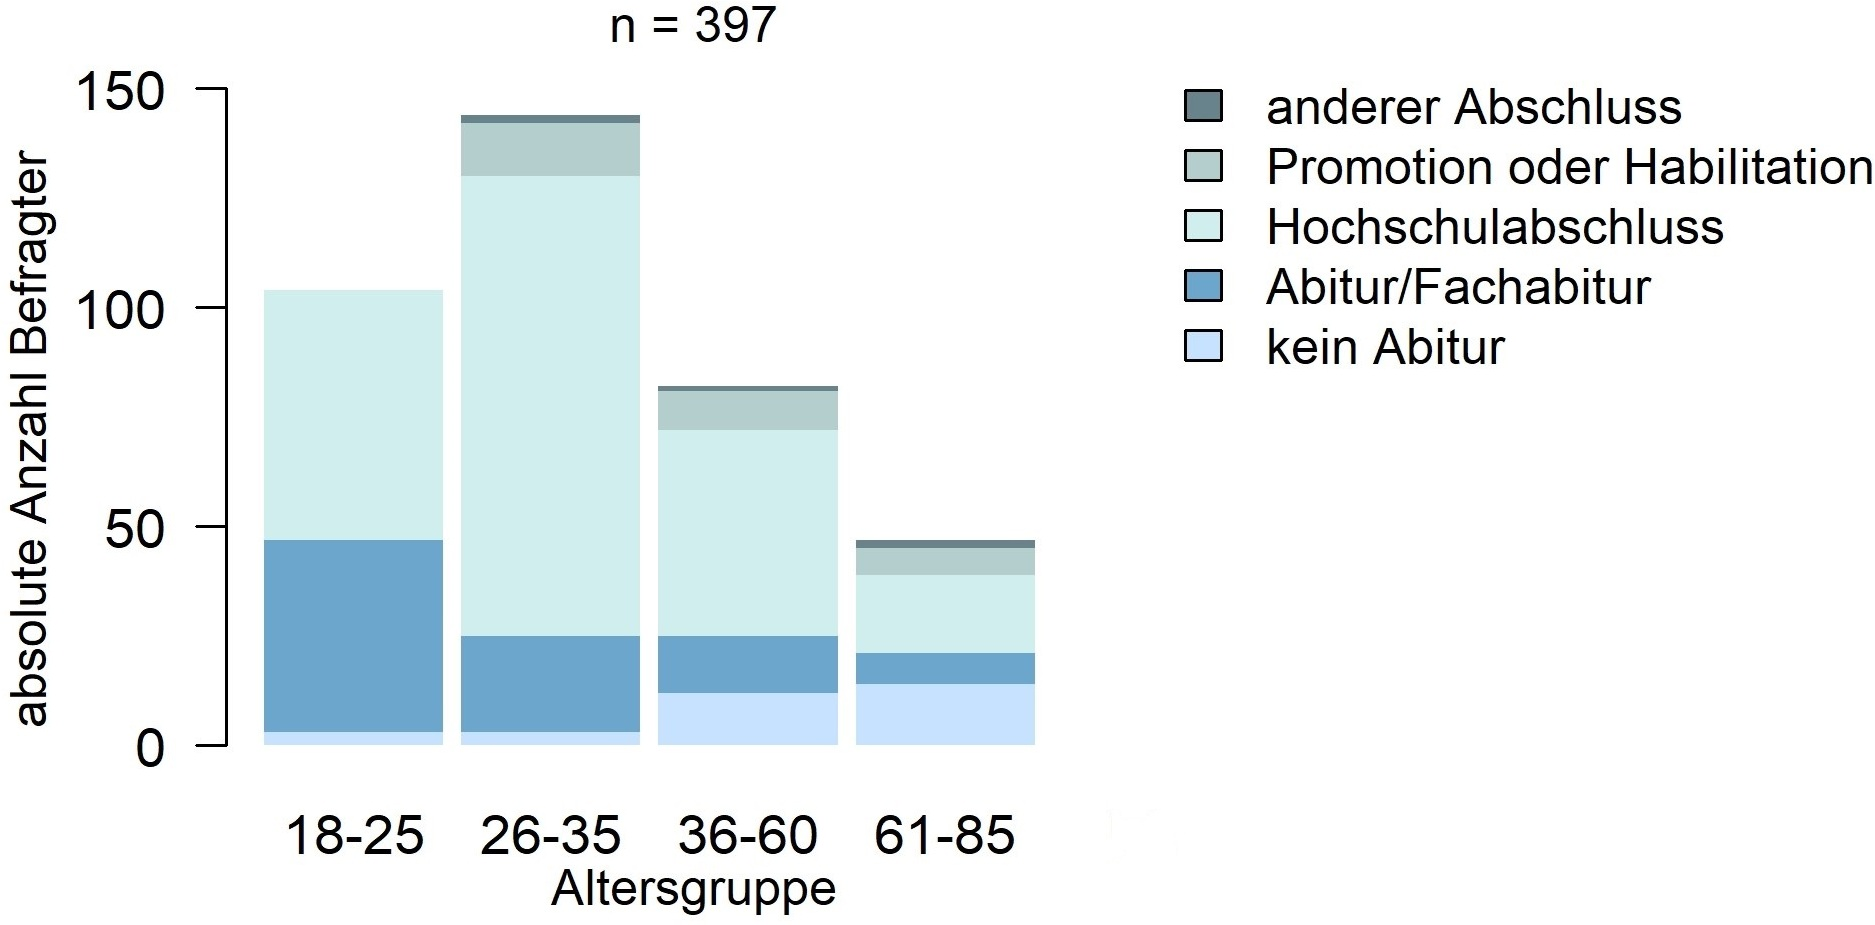
\includegraphics[width=\textwidth]{BildungNachAlter.jpg}
\caption{Bildungsstand der Befragten nach ihrer Altersgruppe}
\label{pic:BildungNachAlter}
\end{figure}
 
Die Aufschlüsselung nach Altersgruppen macht deutlich, dass sich Personen ohne Abitur vor allem unter den Befragten über 35 finden. 
Hier haben insgesamt 20~\% kein Abitur, während es bei den unter 36-Jährigen lediglich 2,4~\% sind. 
Schaut man sich nur die über 60-Jährigen Befragten an, zeigt sich, dass hier sogar beinahe 30~\% angeben, kein Abitur zu haben. 
Der Anteil Befragter ohne Hochschulabschluss ist in beiden Altersgruppen zwar dennoch etwa gleich, jedoch liegt dies zum Teil daran, dass die jüngeren Befragten ihr Studium zum Zeitpunkt der Befragung noch nicht abgeschlossen haben.
Das Ungleichgewicht in der Verteilung der Bildungsabschlüsse muss bei der späteren Analyse von Zusammenhängen zwischen der Bewertung und Verwendung der Rektionskasus mit Alter oder Bildung bedacht werden. 

% s. Alter und Bildung.R
Vergleicht man die regionale Herkunft von Befragten mit Hochschulabschluss und Befragten ohne Hochschulabschluss, fallen keine nennenswerten Unterschiede in der Verteilung auf (s. \autoref{table:AnhHerkunftundHSA} im Anhang). 
\subsection{Textaffinität der Berufe der Befragten}
\label{sec:Beruf}
Um eine Auskunft darüber zu erhalten, wie intensiv die Befragten in ihrem jeweiligen Beruf mit Sprache zu tun haben, wurde danach gefragt, wie häufig sie im Beruf längere Texte verfassen oder lesen (\glqq wie häufig verfassen oder lesen Sie in Ihrem Beruf längere Texte wie zum Beispiel Protokolle oder Artikel?\grqq). 
\autoref{pic:SchreibenLesen} zeigt die Verteilung der Antworten. 
\begin{figure}
\centering
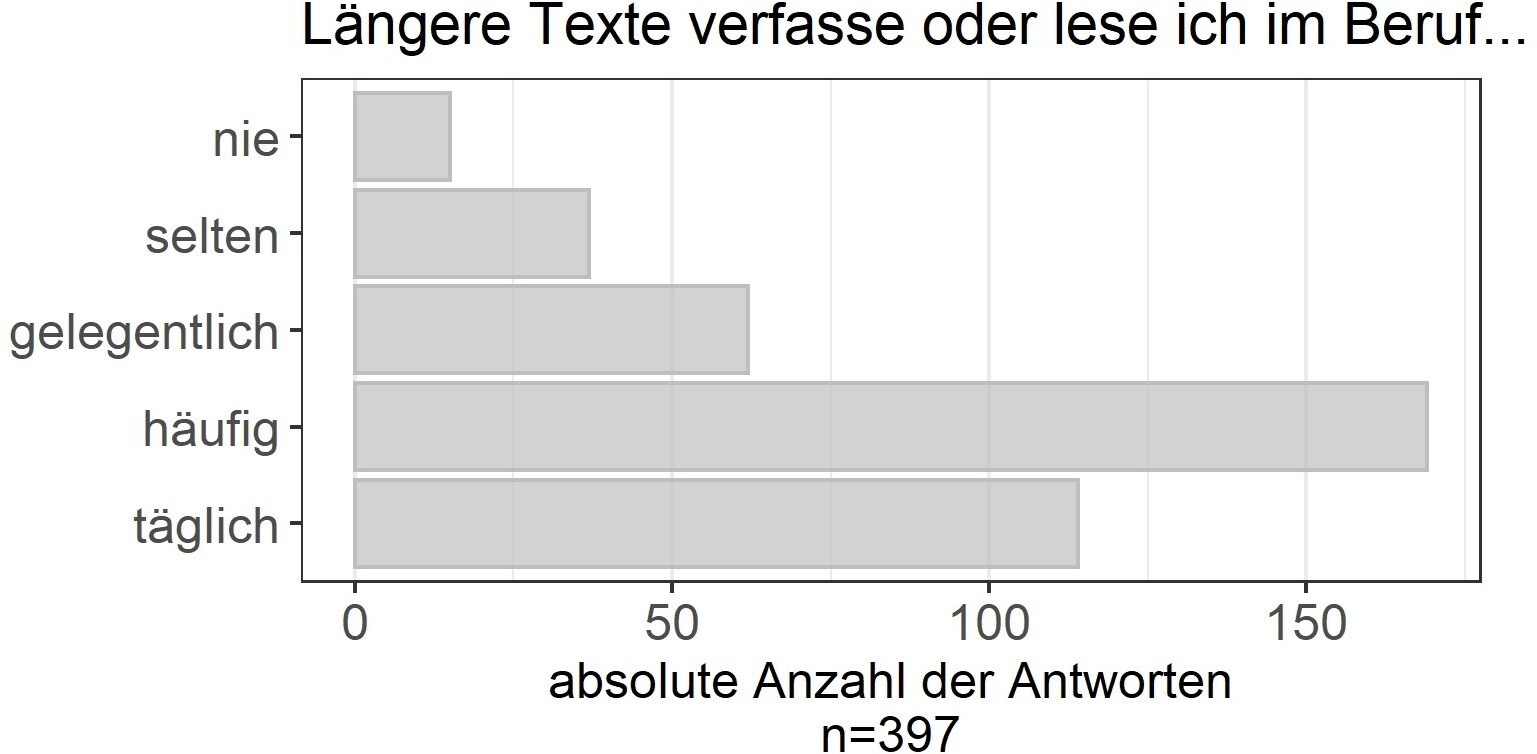
\includegraphics[width=\textwidth]{TextaffinitaetBeruf.jpg}
\caption{Umgang mit längeren Texten im Beruf}
\label{pic:SchreibenLesen}
\end{figure}

Die meisten Befragten geben an, dass sie beruflich häufig oder sogar täglich mit längeren Texten zu tun haben.
Bei 71~\% der Befragten handelt es sich also um beruflich geübte SchreiberInnen und LeserInnen.\footnote{Einzelne TeilnehmerInnen wiesen im Kommentar am Ende des Fragebogens darauf hin, dass die Texte, mit denen sie zu tun haben, größtenteils nicht deutsch sind, sondern bspw. englisch.}
Hierzu zählen etwa LehrerInnen, Studierende und wissenschaftliche MitarbeiterInnen. 
Tatsächlich ist die Gruppe der im Schreiben und Lesen geübten Befragten eventuell sogar noch etwas größer, da Befragte möglicherweise auch außerhalb ihres Berufs mit längeren Texten zu tun haben, etwa wenn sie viele Romane lesen oder einen Vereinsnewsletter betreuen. 
Für die Befragung ist jedoch insbesondere die berufliche Beschäftigung mit längeren Texten relevant, da davon ausgegangen werden kann, dass diese erstens mit einer recht großen Sorgfalt und zweitens mit einer recht hohen Kompetenz in Fragen sprachlicher Normen einhergeht. 

16~\% der Befragten geben an, beruflich gelegentlich mit längeren Texten zu tun zu haben. 
Auch in dieser Gruppe finden sich relativ viele Studierende (14 von 62 Personen) sowie einige Personen, die in den Bereichen Pädagogik/Erziehung arbeiten, und bspw. kaufmännische Berufe.
Nur 52 Befragte (13~\%) geben an, dass sie im Beruf selten oder nie längere Texte verfassen oder lesen. 
Darunter finden sich ebenfalls Studierende, aber auch bspw. Angestellte aus den Bereichen Hotel/Gastronomie und Pflege/Medizin, GrafikerInnen sowie Hausfrauen. 

Für die spätere Untersuchung von Zusammenhängen zwischen Akzeptabilität und Kasuswahl mit der Textaffinität des Berufs lassen sich die Befragten aufteilen in die Gruppe derer, die im Beruf häufig oder sogar täglich mit längeren Texten zu tun haben (Beruf textaffin) und die Gruppe derer, die im Beruf nie bis gelegentlich mit längeren Texten zu tun haben (Beruf nicht textaffin): 
Insgesamt 283 Befragte haben einen textaffinen Beruf, 114 haben einen Beruf, der nicht textaffin ist. 
\subsection{Sprachbewusstheit der Befragten}
\label{sec:Sprachbewusstheit}
Bereits die Angaben zum Umgang mit längeren Texten im Beruf deuten auf eine recht große Sprachaffinität der TeilnehmerInnen hin. 
Um darüber hinaus zu überprüfen, inwiefern sich die Befragten selbst als sprachbewusst, sprachlich sicher und variationstolerant einschätzen, wurde mit drei Likertskalen gearbeitet:
Einer zur Sprachbewusstheit, einer zur Sprachsicherheit sowie einer zur sprachlichen Variation. 
Jede der drei Likertskalen besteht aus mehereren Aussagen (Items), zu denen die Befragten ihre Zustimmung bzw. Ablehnung signalisieren sollen (\autoref{sec:RE}). 
Die Skala zur Sprachbewusstheit enthält folgende drei Aussagen: 
\begin{enumerate}
\item Ich denke häufig über die deutsche Sprache nach.
\item Mit dem Thema Sprache beschäftige ich mich nur sehr selten.
\item Ich interessiere mich für die deutsche Sprache. 
\end{enumerate}

\noindent Die Auswertung der Likertskala zur Sprachbewusstheit zeigt, dass die Befragten überwiegend recht interessiert an Sprache sind. 
\autoref{pic:SB} gibt einen Überblick über die Beantwortung der einzelnen Items der Skala. 
Die genauen Zahlen sind außerdem in \autoref{table:LikertZsfsgAnh} im Anhang zusammengefasst. 
\begin{figure}
\centering
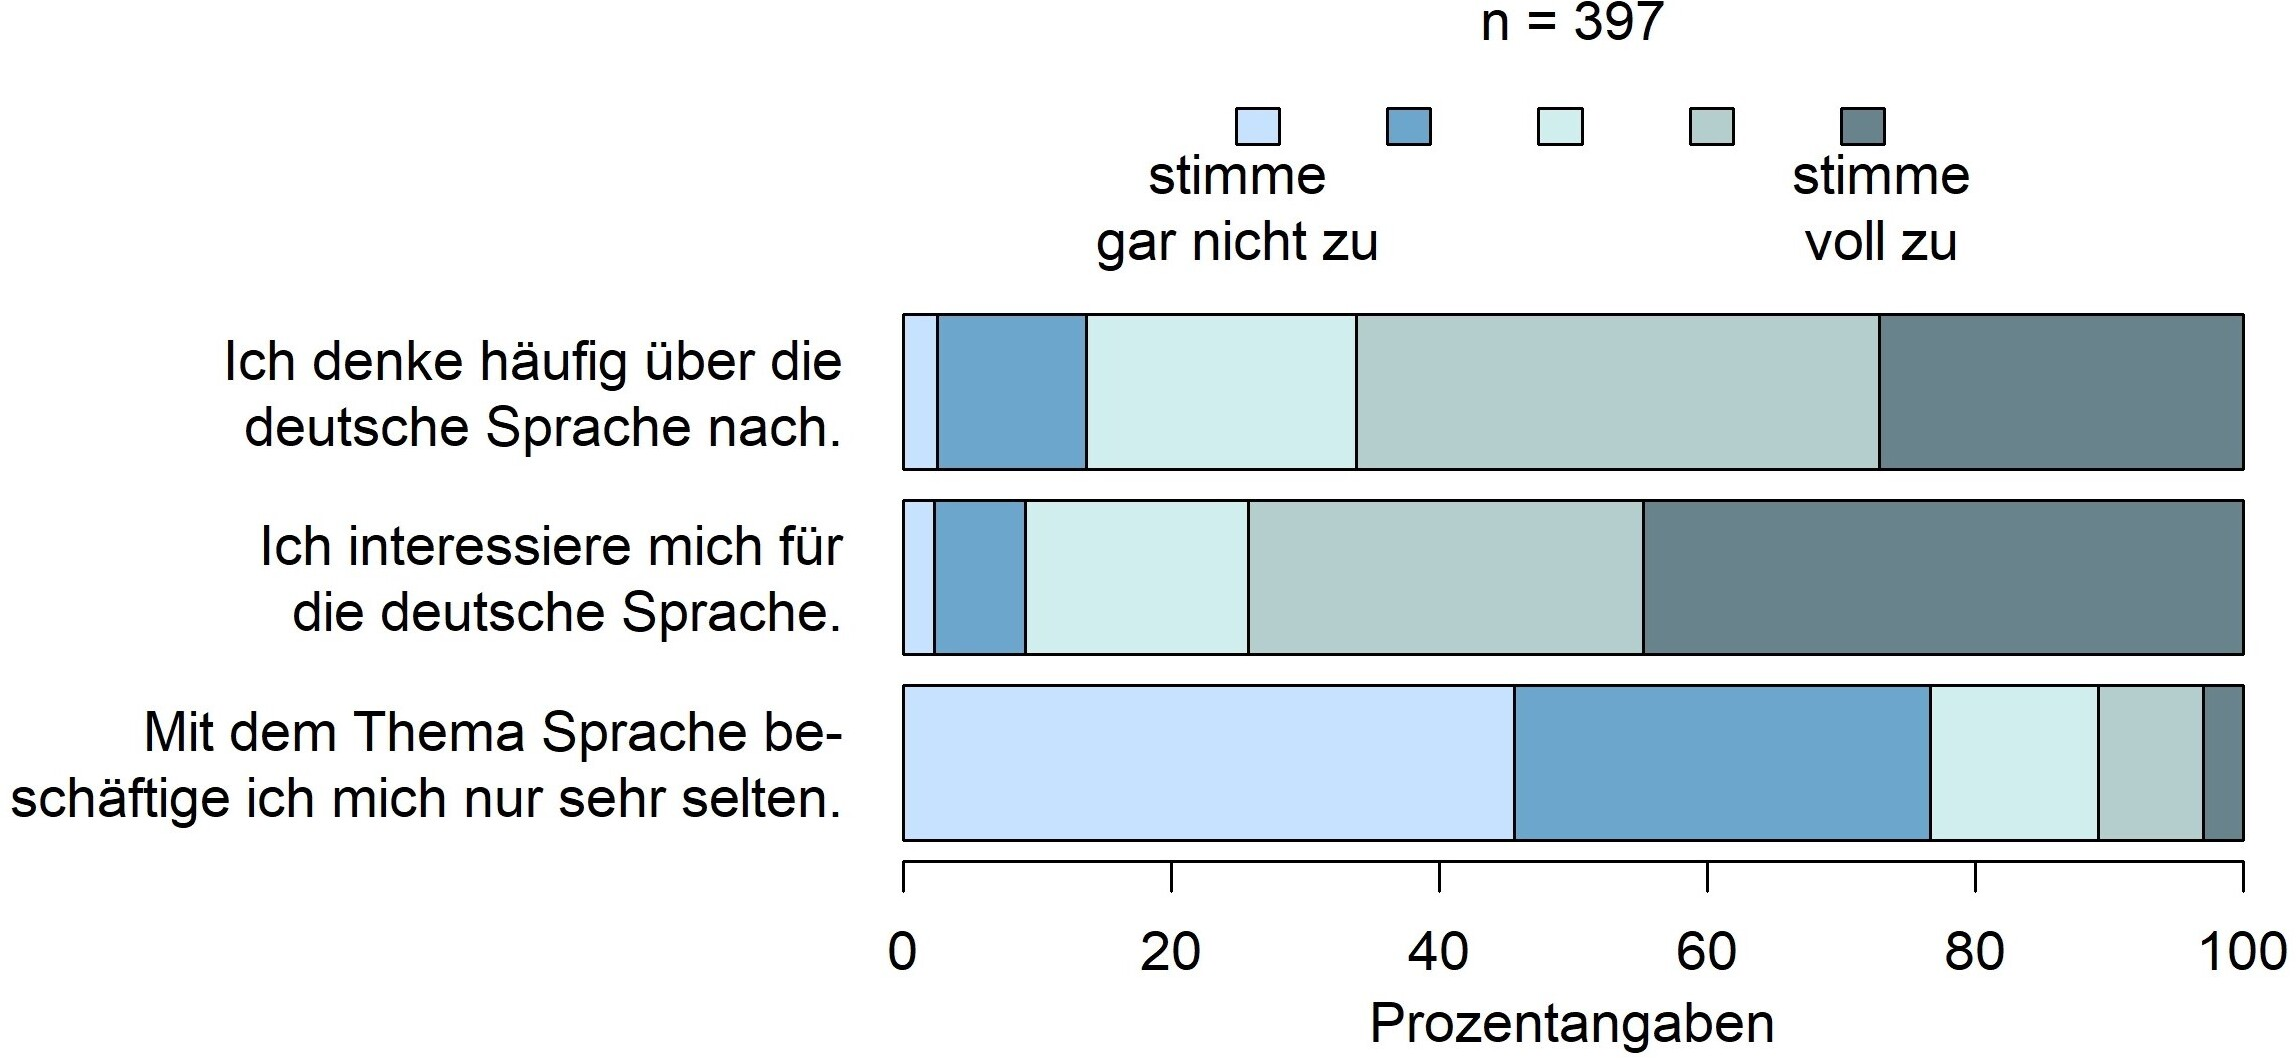
\includegraphics[width=\textwidth]{Sprachbewusstheit.jpg}
\caption{Beantwortung der Likert-Items zur Sprachbewusstheit}
\label{pic:SB}
\end{figure}
 
Zwei Drittel der Befragten stimmen der Aussage zu, häufig über die deutsche Sprache nachzudenken. 
Noch etwas mehr (ungefähr drei Viertel) stimmen zu, dass sie sich für die deutsche Sprache interessieren. 
Die Aussage, dass sie sich nur sehr selten mit dem Thema Sprache beschäftigen, verneinen beinahe 80~\%. 
Dass an der Umfrage vor allem sprachinteressierte Personen teilnahmen, liegt mit Sicherheit in erster Linie daran, dass sie als Umfrage zu einem sprachbezogenen Thema angekündigt wurde. 
\subsection{Selbsteinschätzung der Sprachsicherheit der Befragten}
\label{sec:Sprachsicherheit}
Die meisten TeilnehmerInnen schätzen nicht nur ihr Interesse für Sprache, sondern auch ihre sprachliche Sicherheit recht hoch ein, wie \autoref{pic:SK} zeigt (s. zusätzlich \autoref{table:LikertZsfsgAnh} im Anhang). 
Die Likertskala zu diesem Aspekt fragt insbesondere ab, wie die eigenen Kompetenzen im Bereich Grammatik und Rechtschreibung eingestuft werden. 
Sie besteht aus folgenden drei Aussagen: 
\begin{enumerate}
\item Ich bin bei sprachlichen Fragen häufig unsicher.
\item Wenn jemand eine Frage zu Grammatik oder Rechtschreibung hat, kann ich meistens weiterhelfen.
\item  Ich kenne mich gut mit der deutschen Grammatik aus.
\end{enumerate}

Nur 6,5~\% der Befragten stimmen der Aussage zu, sich bei sprachlichen Fragen häufig unsicher zu fühlen. 
80~\% meinen, Fragen zu Grammatik und Rechtschreibung meist beantworten zu können und 75~\% geben an, sich gut mit der Grammatik auszukennen. 
8 bzw. 7~\% stimmen den Aussagen nicht zu, dass sie sich mit der Grammatik auskennen bzw. bei sprachlichen Fragen weiterhelfen können. 
An der Studie nahmen also durchaus auch Personen teil, die ihr Wissen über Grammatik und Rechtschreibung als gering einschätzen, diese sind allerdings in der Unterzahl.
\begin{figure}[htb]
\centering
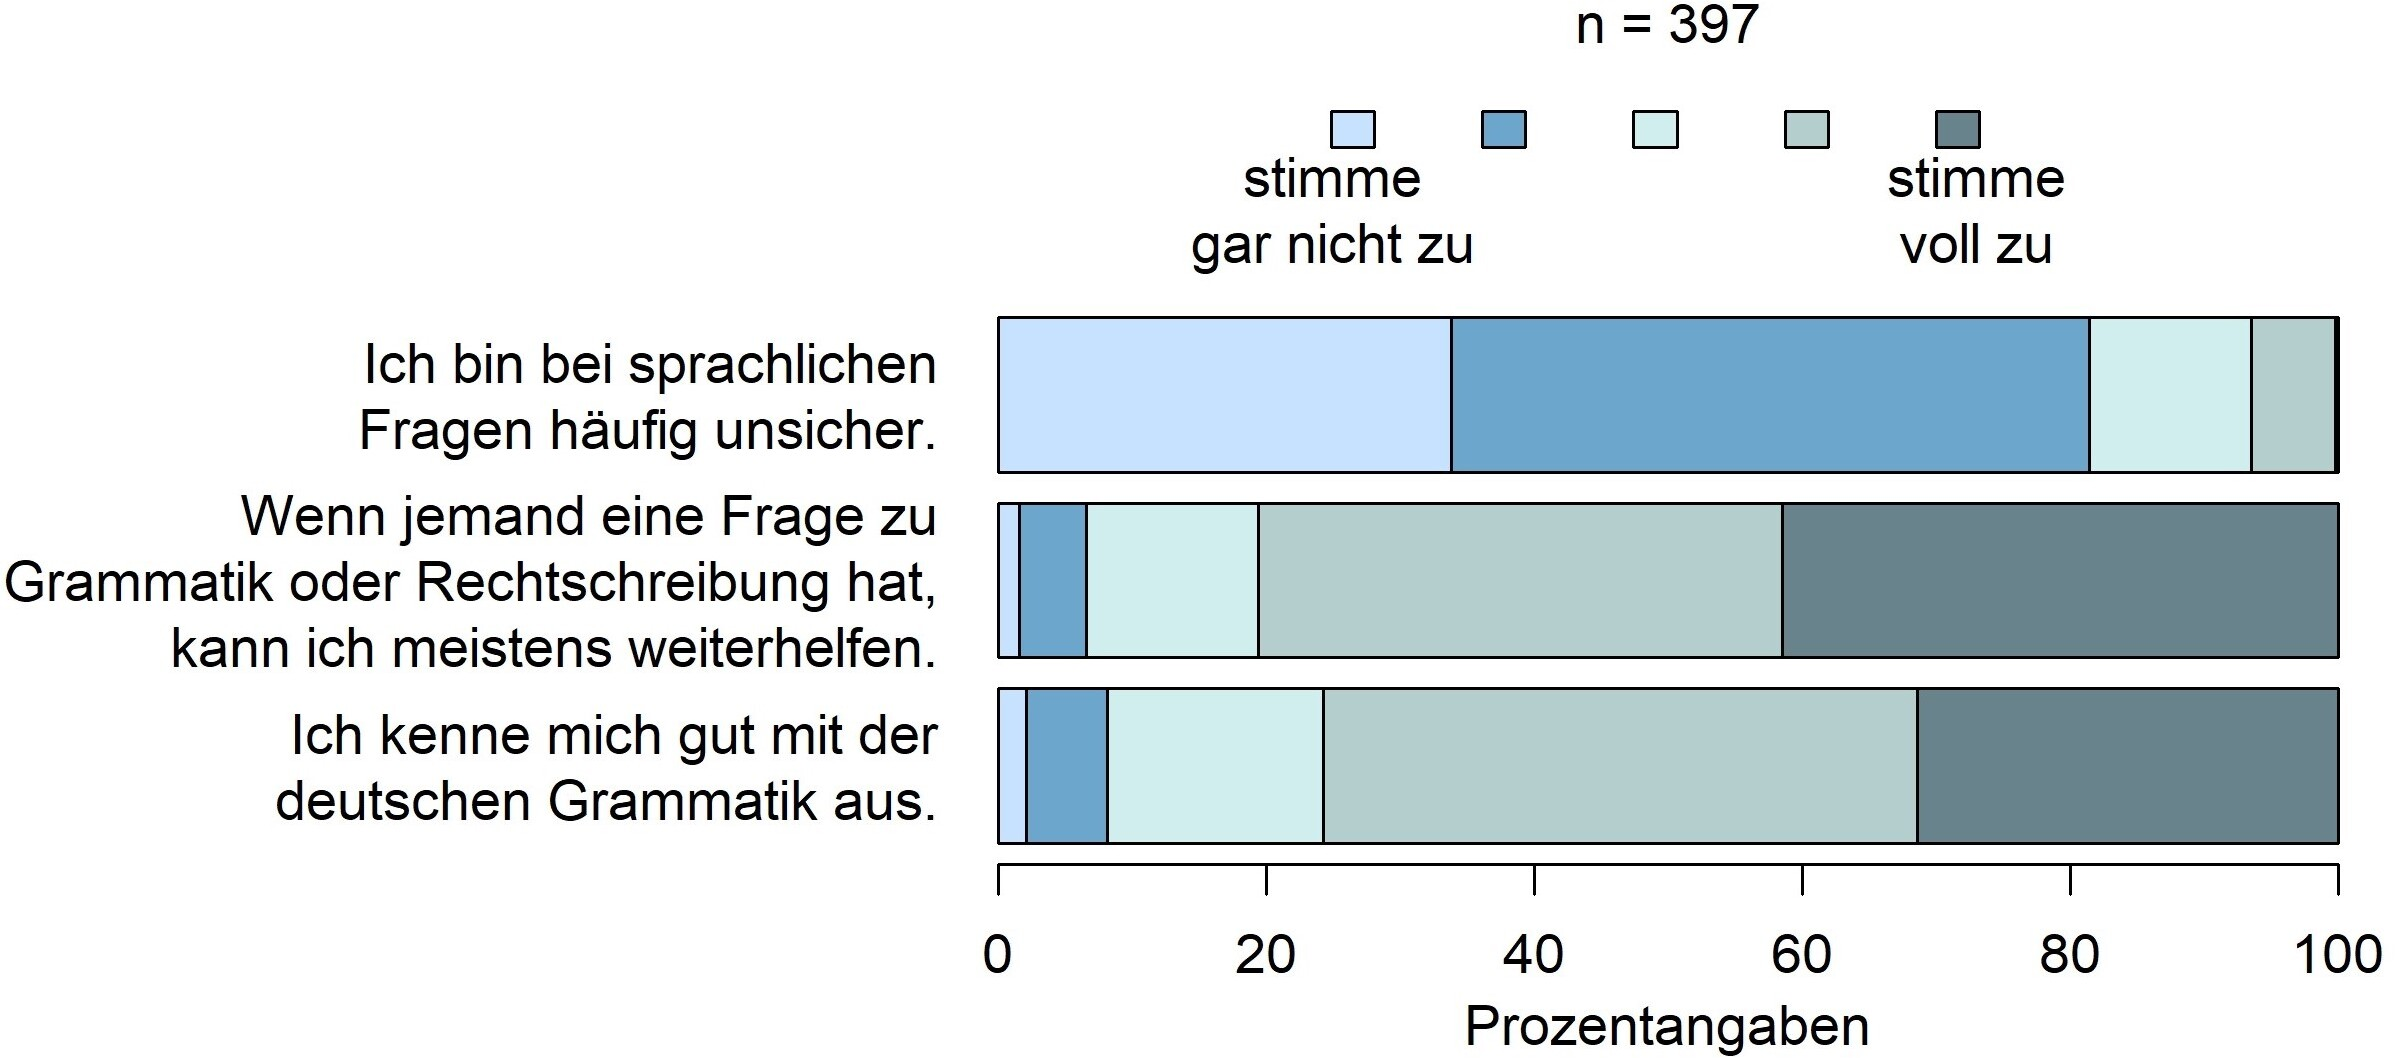
\includegraphics[width=\textwidth]{Sprachkompetenz.jpg}
\caption{Beantwortung der Likert-Items zur Sprachsicherheit}
\label{pic:SK}
\end{figure}

Um zu überprüfuen, inwiefern sich die Selbsteinschätzung der eigenen Sprachsicherheit auf die Angaben im Akzeptabilitätstest und im Produktionsexperiment auswirkt, können die Befragten in zwei Gruppen aufgeteilt werden: 
diejenigen, die ihre sprachliche Sicherheit hoch einschätzen, und diejenigen, die ihre sprachliche Sicherheit gering einschätzen. 
Hierfür muss zunächst das negative Item der Likertskala zur Sprachsicherheit, \glqq ich bin bei sprachlichen Fragen häufig unsicher\grqq, umgepolt werden. 
Die Umpolung hat zur Folge, dass ein hoher Zustimmungswert auch bei diesem Item als Hinweis auf eine hohe Einschätzung der eigenen sprachlichen Sicherheit gedeutet werden kann (\autoref{sec:RE}). 
Anschließend kann der Mittelwert der Zustimmung zu den drei Items der Skala gebildet werden, an dem abgelesen werden kann, wie stark eine befragte Person der Skala insgesamt zustimmt. 
Befragte mit durchschnittlichen Zustimmungswerten von über drei bilden die Gruppe derer, die ihre Sprachsicherheit hoch einschätzen (abgekürzt mit Ss+). 
Befragte mit Durchschnittswerten von drei oder weniger bilden die Gruppe derer, die ihre Sprachsicherheit gering einschätzen (abgekürzt mit Ss--). 
In der Gruppe Ss+ befinden sich 344 Befragte, in der Gruppe Ss-- nur 53. 

Wichtig ist, dass mit der Likertskala die Selbsteinschätzung der Befragten gemessen wird, nicht ihre tatsächliche Sicherheit. 
Dass es hier Diskrepanzen geben kann, zeigt etwa eine Studie von \citet{Gartig2010}:
Hier schätzten auch Befragte, die in einem Rechtschreibtest schlecht abschnitten, ihre eigenen Deutschkenntnisse größtenteils als gut oder sehr gut ein \citep[s.][12--13]{Gartig2010}. 

Die Selbsteinschätzung der sprachlichen Sicherheit korreliert zu einem gewissen Grad mit der in \autoref{sec:Beruf} thematisierten Textaffinität des Berufs. 
Wie \autoref{table:SprachwissenundBeruf} zeigt, ist der Anteil an Befragten mit einem textaffinen Beruf unter denen, die ihre Sprachsicherheit hoch einschätzen, höher als unter denen, die ihre Sprachsicherheit gering einschätzen. 
Jedoch hat auch rund die Hälfte der Personen, die ihre Kompetenzen im Bereich Grammatik und Rechtschreibung gering einschätzen, im Beruf häufig oder täglich mit längeren Texten zu tun. 

\begin{table}
\centering
\begin{tabular}{lrrrr}
\multicolumn{1}{c}{\textbf{}} & Sprachsicherheit hoch eingeschätzt & Sprachsicherheit gering eingeschätzt \\
\midrule
Beruf textaffin               & 255                                             & (74 \%)                                             & 28                                               & (53 \%)                                               \\
Beruf nicht textaffin         & 89                                              & (26 \%)                                             & 25                                               & (47 \%)                                               \\
gesamt                        & 344                                             & (100 \%)                                            & 53                                               & (100 \%)                                              \\ 
\end{tabular}
\caption{Zusammenhang zwischen der Selbsteinschätzung der Sprachsicherheit und der Textaffinität des Berufs}
\label{table:SprachwissenundBeruf}
\end{table}

% Änderung Anfang
Bezogen auf die gesamte Befragtengruppe lässt sich damit festhalten, dass 64 \% der TeilnehmerInnen ihre Sprachsicherheit hoch einschätzen und einen textaffinen Beruf ausüben, während 22 \% aller Befragten ihre Sprachsicherheit hoch einschätzen, ohne einen textaffinen Beruf zu haben.
7 \% der Befragten schätzen die eigene Sprachsicherheit gering ein und gehen einem textaffinen Beruf nach, 6 \% hingegen schätzen die eigene Sprachsicherheit gering ein und haben keinen textaffinen Beruf. %Änderung Ende
\subsection{Variationstoleranz der Befragten}
\label{sec:Variationstoleranz}
Die Likertskala zur Einstellung gegenüber Variation zielt darauf ab, herauszufinden, inwiefern die Befragten verschiedene Aspekte der Standardsprachideologie und der Sprachverfallsideologie vertreten, wie etwa die Auffassung, dass nur eine Variante korrekt sein kann (s. \autoref{pic:VT}, vgl. \autoref{sec:MetapragmatikVariationWandel}). 
Sie enthält folgende vier Aussagen: 
\begin{enumerate}
\item Je nach Region können verschiedene Sprachformen richtig sein. 
\item Es ist gut, dass sich der Duden dem aktuellen Sprachgebrauch anpasst.
\item In der Sprache sollten feste Regeln vorschreiben, was richtig und was falsch ist. 
\item Die deutsche Grammatik verfällt immer mehr. 
\end{enumerate}

\begin{figure}[htb]
\centering
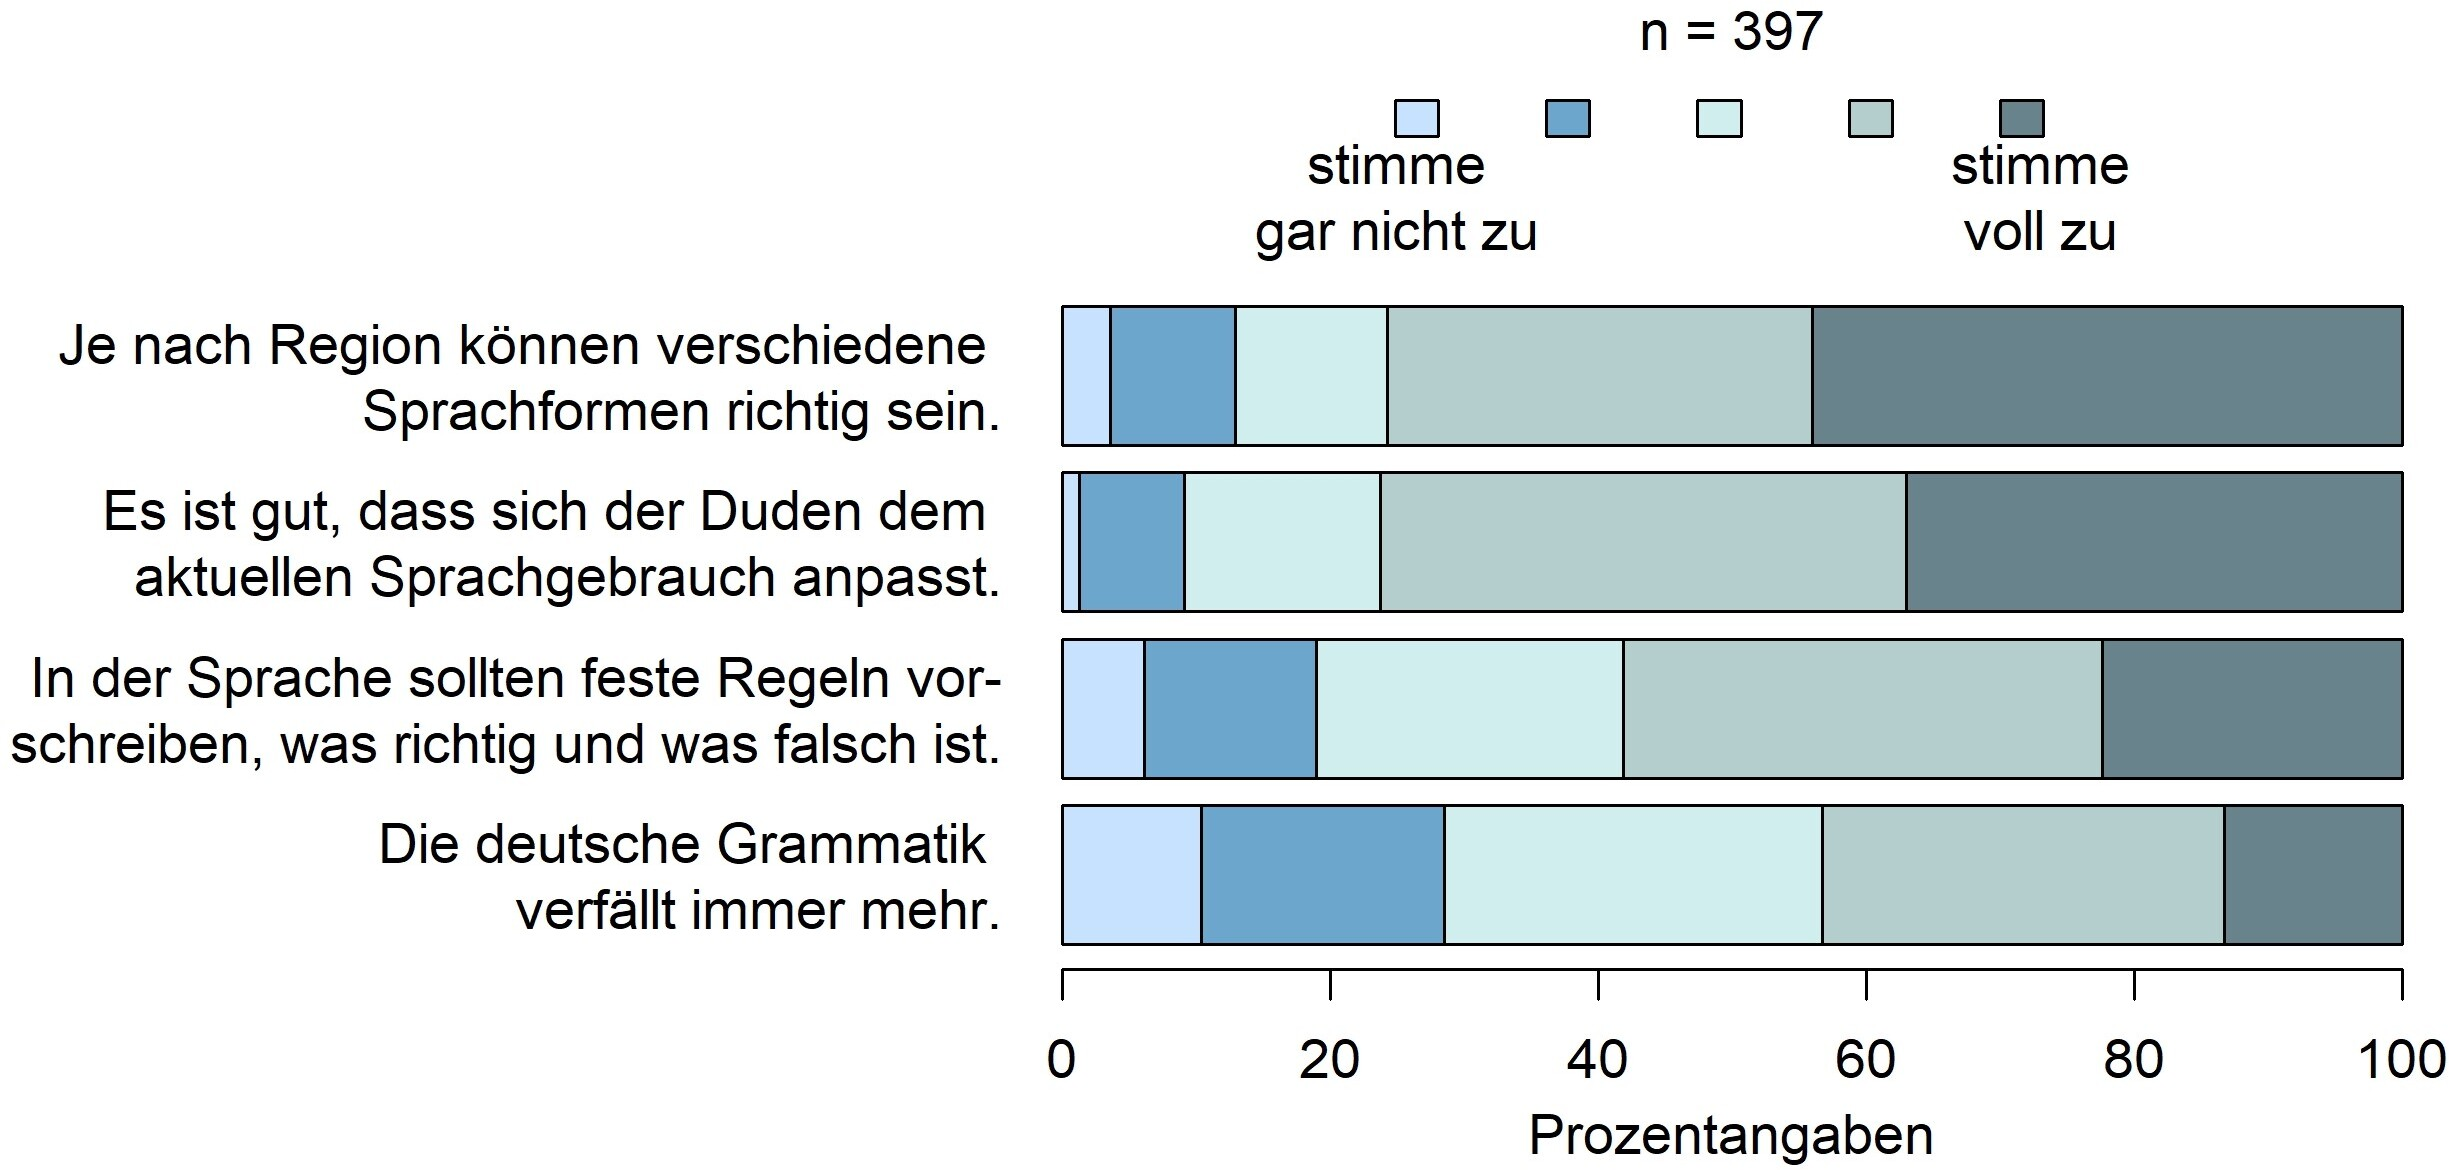
\includegraphics[width=\textwidth]{Variationstoleranz.jpg}
\caption{Beantwortung der Likert-Items zur Variationstoleranz}
\label{pic:VT}
\end{figure}

Hier zeigt sich auf der einen Seite eine Toleranz gegenüber regionaler sowie diachroner Variation: Rund drei Viertel der Befragten stimmen zu, dass je nach Region verschiedene sprachliche Formen richtig sein können (für die genauen Zahlen s. auch \autoref{table:LikertZsfsgAnh} im Anhang). Beinahe ebenso viele befürworten, dass der Duden sich dem aktuellen Sprachgebrauch anpasst. 
Auf der anderen Seite zeigen sich aber auch der Wunsch nach präskriptiven Regeln und die Vorstellung, die Sprache verfalle: 58~\% der Befragten stimmen der Aussage zu, feste Regeln sollten in der Sprache vorschreiben, was richtig und was falsch ist. 
43~\% finden, dass die deutsche Grammatik immer mehr verfällt.
Die Ideologie der sprachlichen Einheitlichkeit und die Vorstellung eines drohenden Verlusts dieser Einheitlichkeit sind unter den Befragten also recht verbreitet. 

Für die Analyse von Zusammenhängen zwischen der Variationstoleranz der Befragten und ihren Angaben im Akzeptabilitätstest sowie ihrer Kasuswahl können zwei Gruppen gebildet werden.
Hierfür werden wieder zunächst die negativen Items der Likertskala zur Variationstoleranz umgepolt, sodass ein hoher Zustimmungswert bei allen Items für eine hohe Zustimmung zu Variation steht (\autoref{sec:RE}). 
Die Items, die dafür umgepolt werden müssen, sind \glqq in der Sprache sollten feste Regeln vorschreiben, was richtig und was falsch ist\grqq{} und \glqq die deutsche Grammatik verfällt immer mehr\grqq.
Befragte, die auf der Likertskala zur Variationstoleranz einen durchschnittlichen Wert von drei oder weniger erzielen, bilden die wenig variationstolerante Gruppe, im Folgenden abgekürzt mit Vt--. 
Diese Gruppe besteht aus insgesamt 169 Befragten. 
Befragte mit Likertwerten von über drei bilden die variationstolerante Gruppe, im Folgenden abgekürzt mit Vt+. 
Diese Gruppe umfasst 228 Befragte. 
Beide Gruppen unterscheiden sich kaum, was ihre Zusammensetzung nach soziodemografischen Merkmalen wie Alter, regionale Herkunft oder Bildungsstand angeht (s. \autoref{table:AnhAlterundVt} bis \autoref{table:AnhBildungundVt} im Anhang). 
Alle Differenzen liegen im einstelligen Prozentbereich. 
\subsection{Zusammenfassung zur Zusammensetzung der Befragtengruppe}
\label{sec:ZsfsgBefragte}
Die soziodemografischen Angaben der Befragten lassen sich wie folgt zusammenfassen:
Die TeilnehmerInnen der Studie sind überwiegend jung und weiblich, stammen aus Norddeutschland, sprechen keinen Dialekt, verfügen über einen hohen Bildungsabschluss und üben einen Beruf aus, in dem sie häufig mit längeren Texten zu tun haben.
Teilweise gibt es Überschneidungen zwischen den soziodemografischen Merkmalen. 
So finden sich in der Gruppe der 18- bis 25-Jährigen besonders viele weibliche Befragte. 
Unter den über 60-Jährigen ist der Anteil an Befragten aus Norddeutschland und an Befragten ohne Hochschulabschluss höher als in anderen Altersgruppen. 
DialektsprecherInnen finden sich vor allem unter Befragten aus süddeutschen Bundesländern. 

\autoref{pic:Likertskalen} fasst die Ergebnisse der Likertskalen zu Sprachbewusstheit, Sprachsicherheit und Variationstoleranz zusammen. 
Dargestellt sind die Likertwerte aller Befragten für die drei Skalen. 
Für jede befragte Person sind also drei Werte abgebildet, die jeweils  dem Durchschnitt der Zustimmung zu den einzelnen Items einer Skala entsprechen.
Die Aussagen, bei denen Zustimmung bedeutet, dass das abgefragte Konzept wenig ausgeprägt ist, werden zur Berechnung dieser Durchschnittswerte zuvor umgepolt, wie  in \autoref{sec:RE} beschrieben. 
Ein Beispiel für ein solches Item ist die dritte Aussage auf der Likertskala zur Sprachbewusstheit (\glqq mit dem Thema Sprache beschäftige ich mich nur sehr selten\grqq).
Wenn eine Person also bspw. auf der Likertskala zur Sprachbewusstheit den ersten beiden Items voll zustimmt und dem dritten Item gar nicht zustimmt, so erhält sie für die Sprachbewusstheit den Wert 5. 
\begin{figure}
\centering
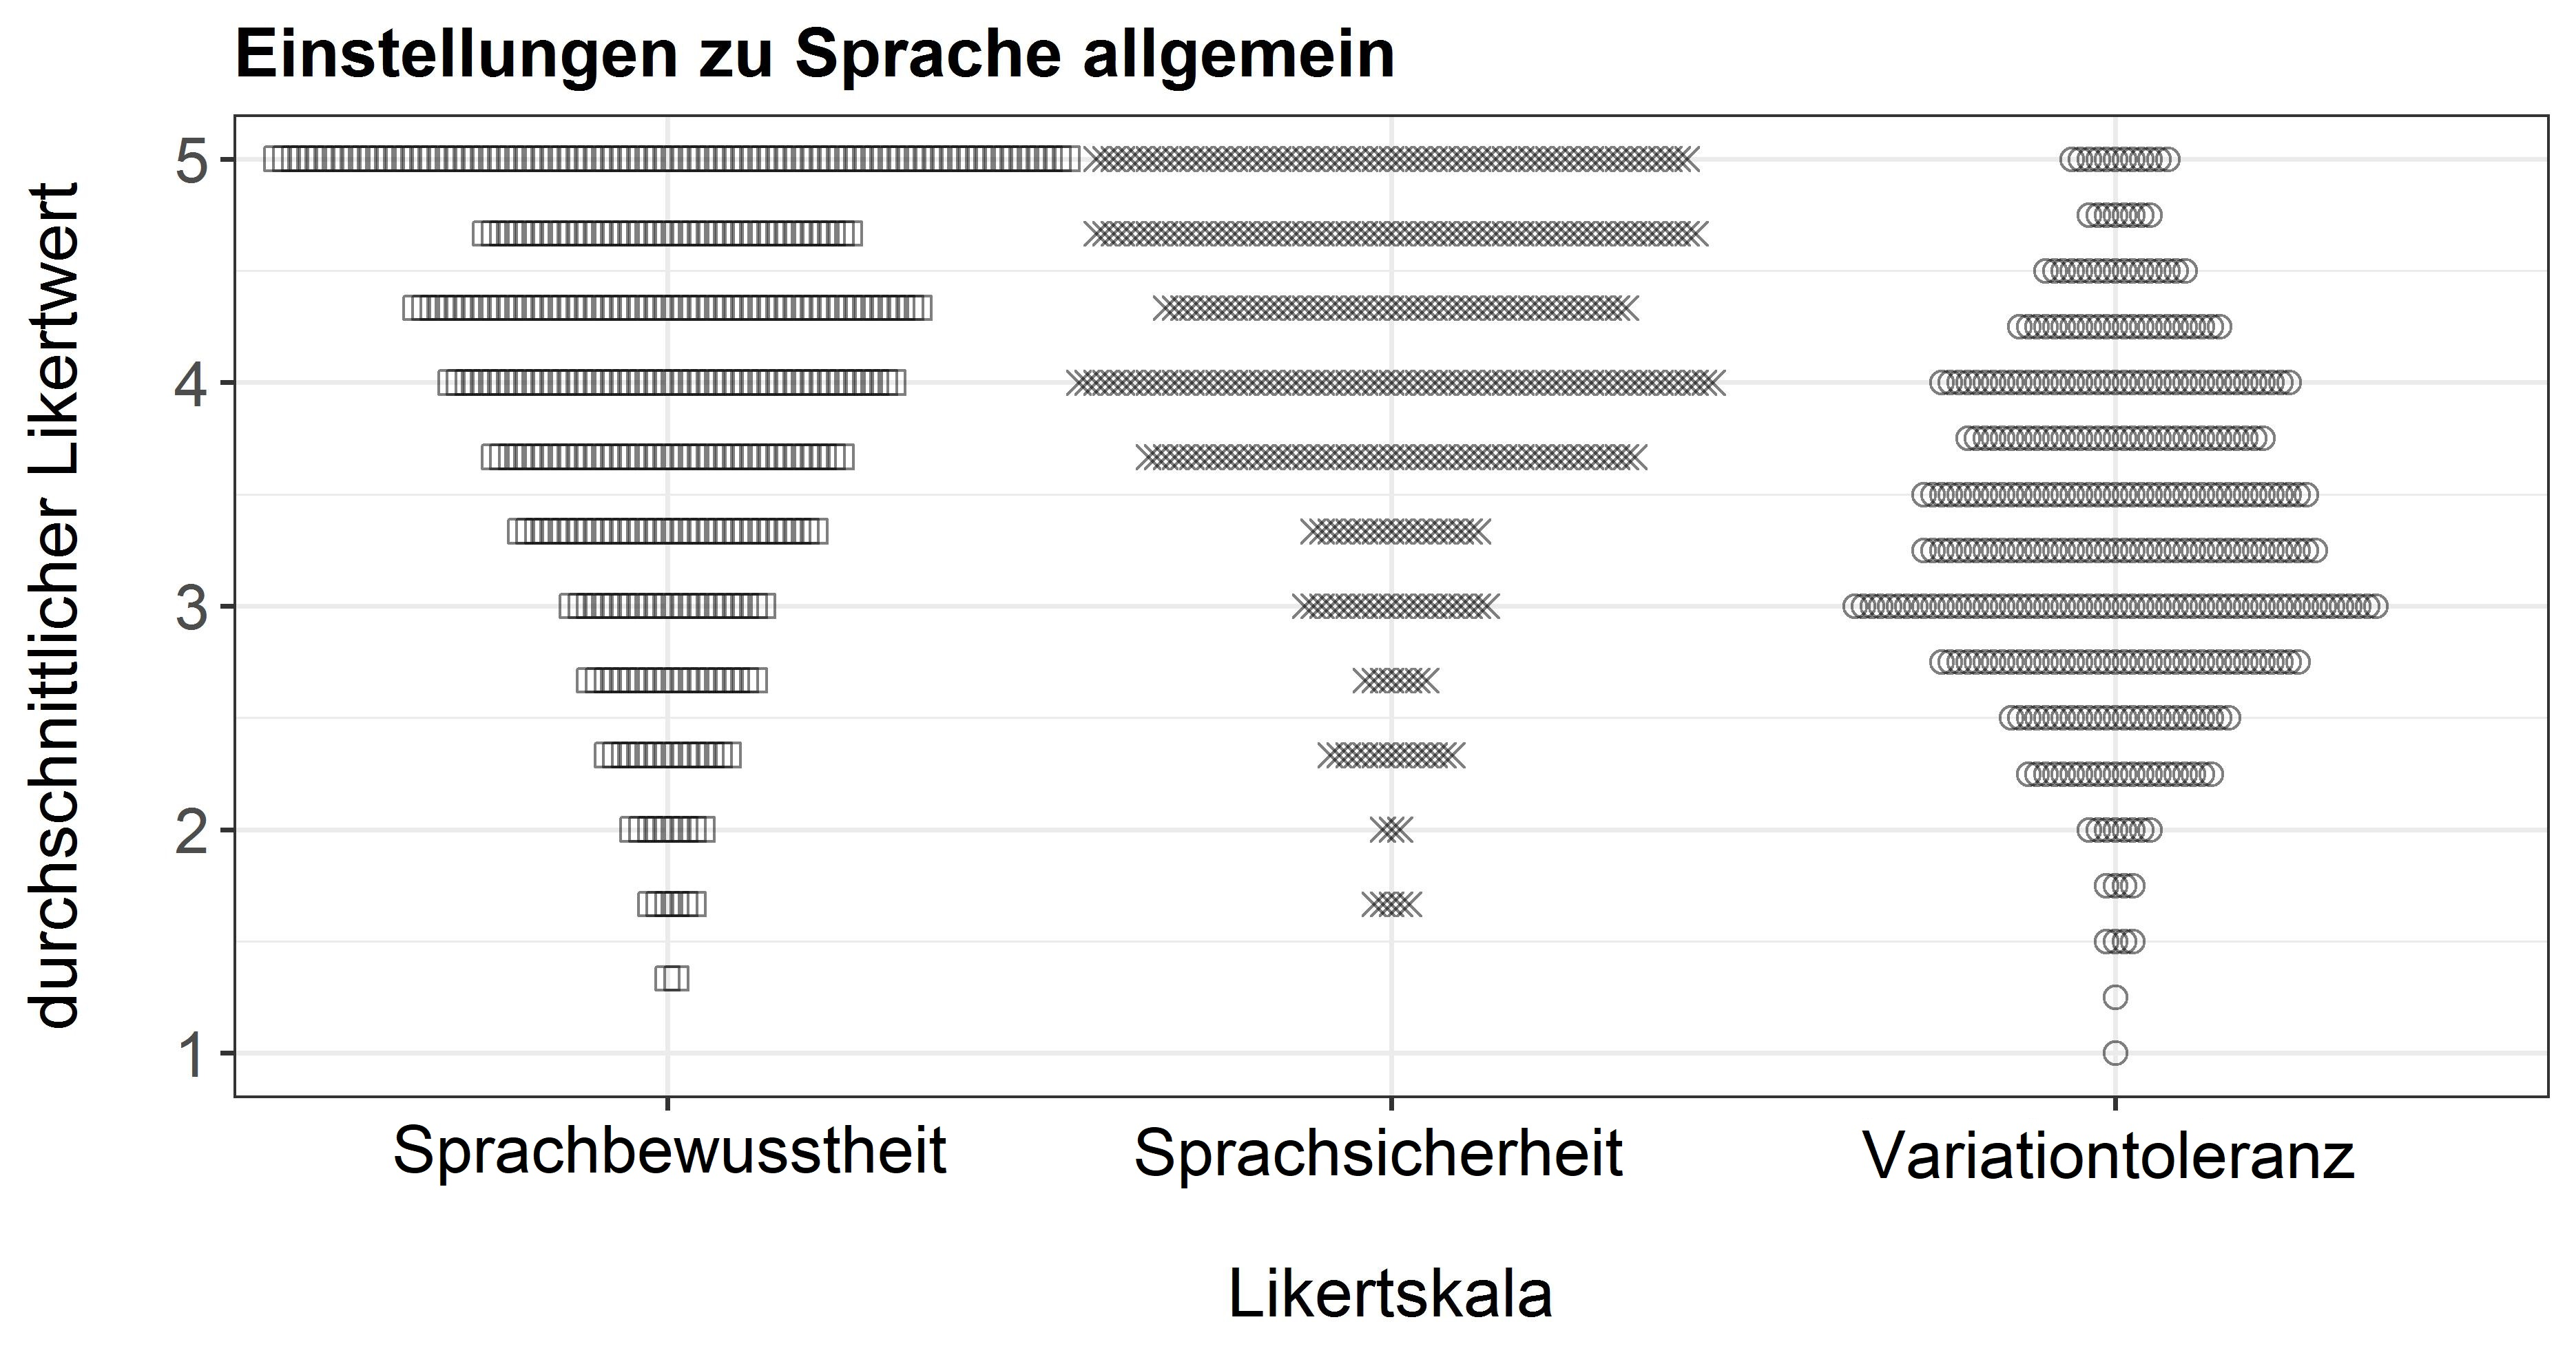
\includegraphics[width=\textwidth]{likertbee.jpg}
\caption{Likertwerte der Befragten zu Sprachbewusstheit, Sprachsicherheit und Variationstoleranz}
\label{pic:Likertskalen}
\end{figure}
 
An den durchschnittlichen Likertwerten lässt sich zusammenfassend ablesen, dass das Interesse an Sprache sowie die Einschätzung der eigenen Sprachsicherheit unter den Befragten recht hoch sind:
Auf den Skalen zu Sprachbewusstheit und Sprachsicherheit erreichen die meisten Befragten hohe durchschnittliche Likertwerte zwischen 4,0 und 5,0. 
Nur wenige Befragte haben hier durchschnittliche Likertwerte von unter 3,0. 
Die Toleranz für sprachliche Variation liegt hingegen bei den meisten Befragten im mittleren Bereich. 
Auch hier finden sich jedoch mehr hohe als niedrige Durchschnittswerte, was auf eine insgesamt eher hohe Variationstoleranz in der Befragtengruppe hindeutet.  
\section{Assoziationen zu den Rektionsvarianten}
\label{sec:ErgAss}
Im Assoziationsteil des Fragebogens wurden explizite metapragmatische Äußerungen zu den Rektionsvarianten von \wegen, \waehrend, \dank{} und \gegenueber{} erhoben. 
Sie wurden einerseits mithilfe von semantischen Differenzialen erfragt und andererseits mithilfe von offenen Fragen nach Assoziationen. 
Für diesen Teil des Fragebogens wurden die Befragten auf vier Gruppen aufgeteilt. 
In jeder Gruppe wurden Assoziationen zu beiden Rektionsvarianten einer der untersuchten Präpositionen erhoben (\autoref{sec:Ass}).
\autoref{table:Ass} gibt einen Überblick über die jeweiligen Beispielsätze und die Anzahl der Befragten pro Gruppe. 

\begin{table}
\centering
\begin{tabular}{llr}
\lsptoprule
Präposition & Beispielsätze im Fragebogen                                                                                                               & \multicolumn{1}{l}{Befragte} \\
\midrule
\textit{dank}        & \textit{\begin{tabular}[c]{@{}l@{}}Dank des Brückentags konnte ich ihn besuchen. \\ Dank dem Brückentag konnte ich ihn besuchen.\end{tabular}}     & 96                                                         \\ \tablevspace
\textit{gegenüber}   & \textit{\begin{tabular}[c]{@{}l@{}}Sie hat es gegenüber des Lehrers nicht erwähnt. \\ Sie hat es gegenüber dem Lehrer nicht erwähnt.\end{tabular}} & 101                                                        \\ \tablevspace
\textit{wegen}       & \textit{\begin{tabular}[c]{@{}l@{}}Ich bin wegen dem Starkregen zu spät gekommen.\\ Ich bin wegen des Starkregens zu spät gekommen.\end{tabular}}  & 96                                                         \\ \tablevspace
\textit{während}     & \textit{\begin{tabular}[c]{@{}l@{}}Während dem Telefonat mache ich Notizen. \\ Während des Telefonats mache ich Notizen.\end{tabular}}             & 104                                                        \\ 
\lspbottomrule
\end{tabular}
\caption{Beispielsätze und Anzahl der Befragten in den vier Gruppen im Assoziationstest}
\label{table:Ass}
\end{table}
Im Folgenden werden zunächst die Ergebnisse der semantischen Differenziale dargestellt. 
Die anschließenden Abschnitte wenden sich den freien Assoziationen zu.
\subsection{Ergebnisse der semantischen Differenziale}
\label{sec:ErgSemDiff}
Mithilfe der semantischen Differenziale wurde abgefragt, inwiefern die Befragten die präsentierten Varianten als gebildet, kompetent, freundlich und sympathisch empfinden. 
Hierfür konnten die Befragten die beiden in ihrer Gruppe abgefragten Varianten jeweils auf einer fünfstufigen Skala bewerten. 
An einem Ende der Skala stand etwa \glqq ungebildet\grqq, am anderen \glqq gebildet\grqq{} (\autoref{sec:Ass}). 
%Die Angabe eines Mittelwerts bei Skalen mit nur einem einzelnen Item ist zwar problematisch, in der Spracheinstellungsforschung aber durchaus üblich \citep[vgl. etwa][184]{Plewnia.2011}. 
%Um die Ergebnisse der Studie mit anderen vergleichbar zu machen, wird daher auch hier auf diese Darstellung zurückgegriffen. 
Die Ergebnisse der semantischen Differenziale sind in \autoref{pic:sdsWegen} bis \autoref{pic:sdsGegenueber} in Form von Boxplots dargestellt.
In den Boxplots ist jeweils der Median für die Einschätzung der Varianten auf der semantischen Differenzialskala als fettgedruckte Linie eingezeichnet. 
Zusätzlich sind die Quartile abzulesen: Das untere Ende einer Box entspricht jeweils dem ersten Quartil, das obere Ende dem dritten. 
Das heißt, es liegen jeweils 25~\% der Daten unter dem unteren Rand einer Box und 75~\% unter dem oberen Rand der Box.
Die Spanne der Box entspricht dem Interquartilsabstand (IQR). 
Die Whiskers reichen jeweils bis zu dem Wert in den Daten, der sich noch innerhalb des 1,5-fachen Interquartilsabstands befindet.
Im Folgenden werden zunächst die Ergebnisse zu den Genitivpräpositionen \wegen{} und \waehrend{} besprochen und anschließend die Ergebnisse zu den Dativpräpositionen \dank{} und \gegenueber. 

Betrachtet man die beiden ursprünglichen Genitivpräpositionen \wegen{} und \waehrend{} (s. \autoref{pic:sdsWegen} und \autoref{pic:sdsWaehrend}), fällt zweierlei auf: 
Erstens wird die Genitivrektion in den Statuskategorien \glqq Bildung\grqq{} und \glqq Kompetenz\grqq{} deutlich positiver bewertet als die Dativrektion. 
\object{Während} mit dem Genitiv wird sogar von allen Befragten mit mindestens dem Wert 3 auf der Skala zwischen ungebildet und gebildet bewertet. 
Hinzu kommt, dass die Einschätzung der Bildung bei \waehrend{} plus Dativ der einzige Fall in den semantischen Differenzialen ist, bei dem der höchste Wert, 5, nicht vergeben wurde (s. auch \autoref{table:sdswaehrendAnh} im Anhang). 
VerwenderInnen der Dativrektion bei \waehrend{} werden also von niemandem für sehr gebildet gehalten. 
Zweitens unterscheidet sich die Bewertung der beiden Rektionsvarianten in den Wärmekategorien jeweils kaum.
\begin{figure}
\centering
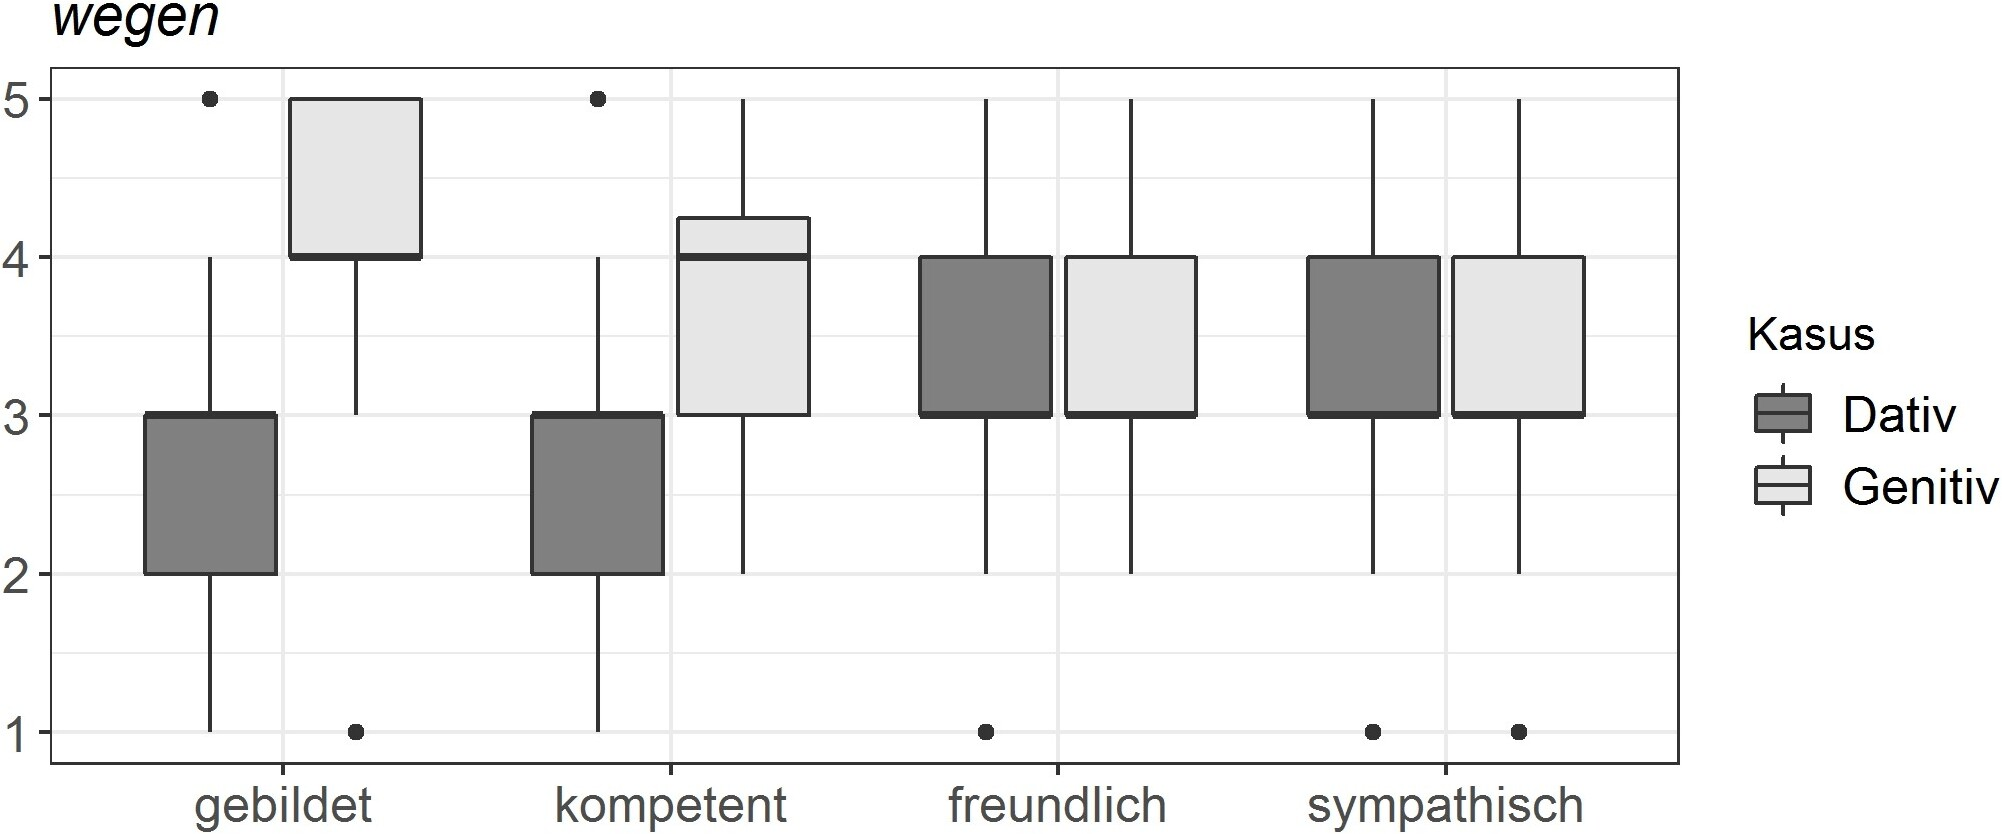
\includegraphics[width=\textwidth]{sdswegenBoxplots.jpg}
\caption{Bewertung der Rektionsvarianten von \wegen}
\label{pic:sdsWegen}
\end{figure}
\begin{figure}
\centering
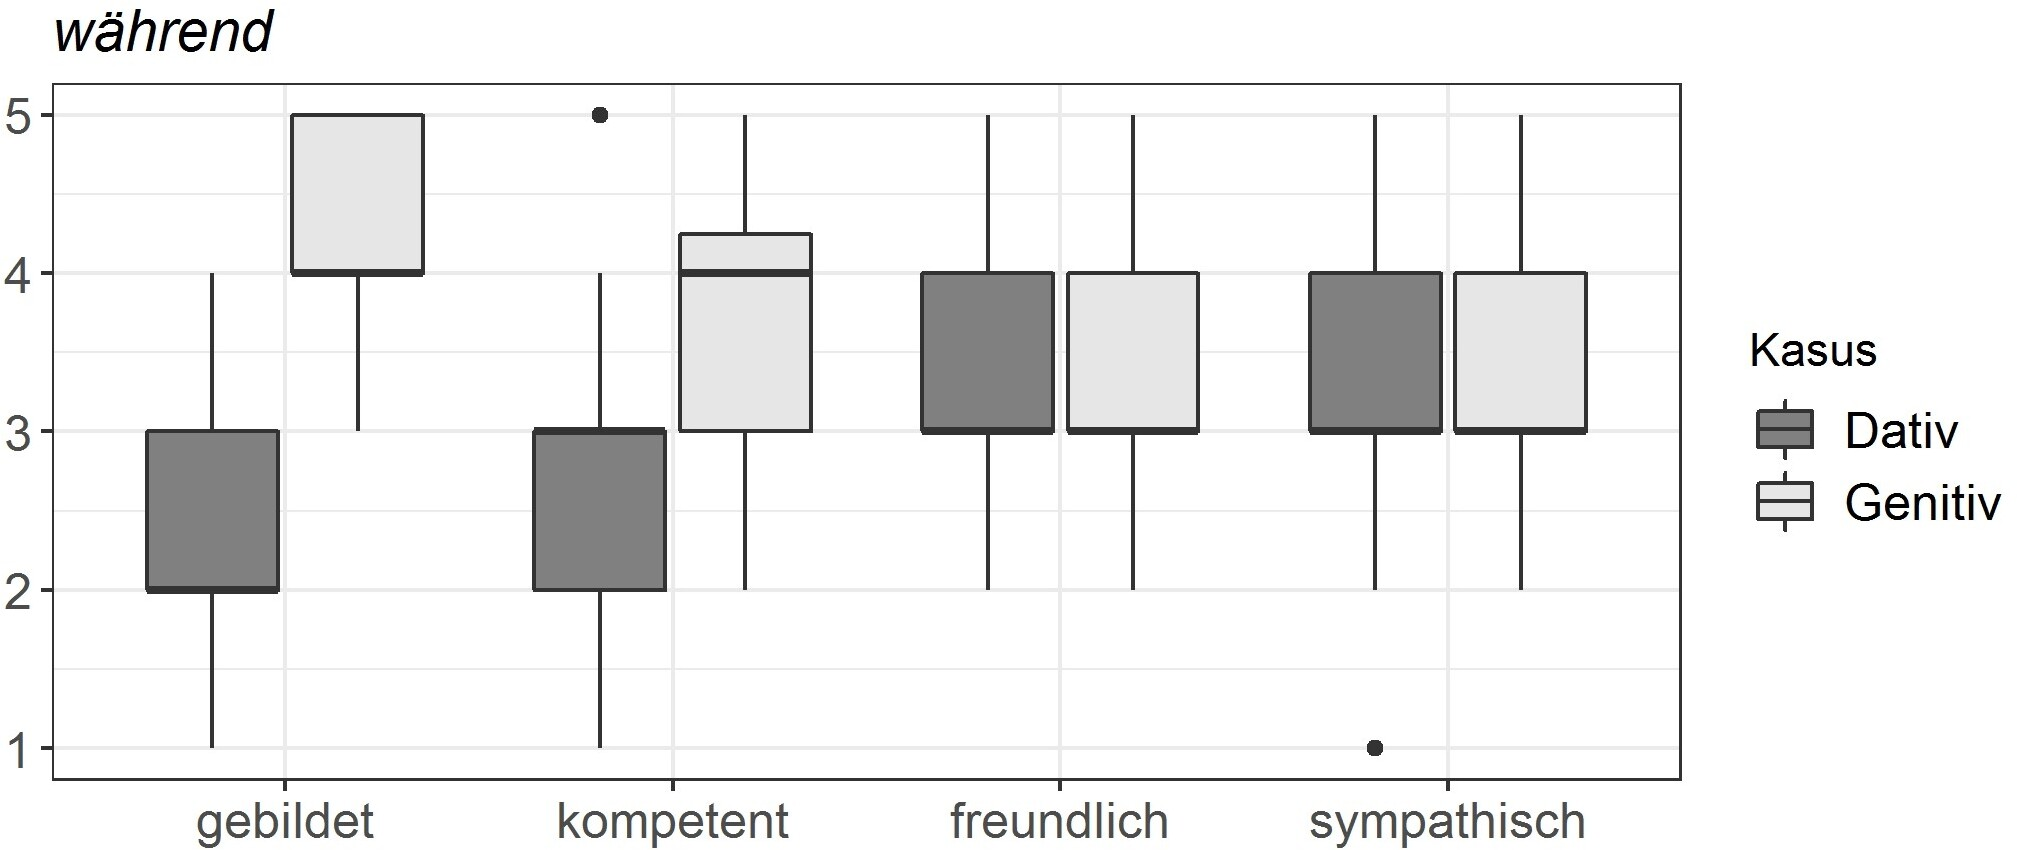
\includegraphics[width=\textwidth]{sdswaehrendBoxplots.jpg}
\caption{Bewertung der Rektionsvarianten von \waehrend}
\label{pic:sdsWaehrend}
\end{figure}
 
In \autoref{pic:sdsDank} ist erkennbar, dass der Genitiv bei \dank{} stark mit den Statuskategorien in Verbindung gebracht wird: 
Der Median liegt sowohl in der Kategorie \glqq Bildung\grqq{} als auch in der Kategorie \glqq Kompetenz\grqq{} bei 5.
Das heißt, mindestens die Hälfte der Befragten hat \dank{} plus Genitiv mit 5, also als sehr gebildet bzw. sehr kompetent bewertet.
\begin{figure}
\centering
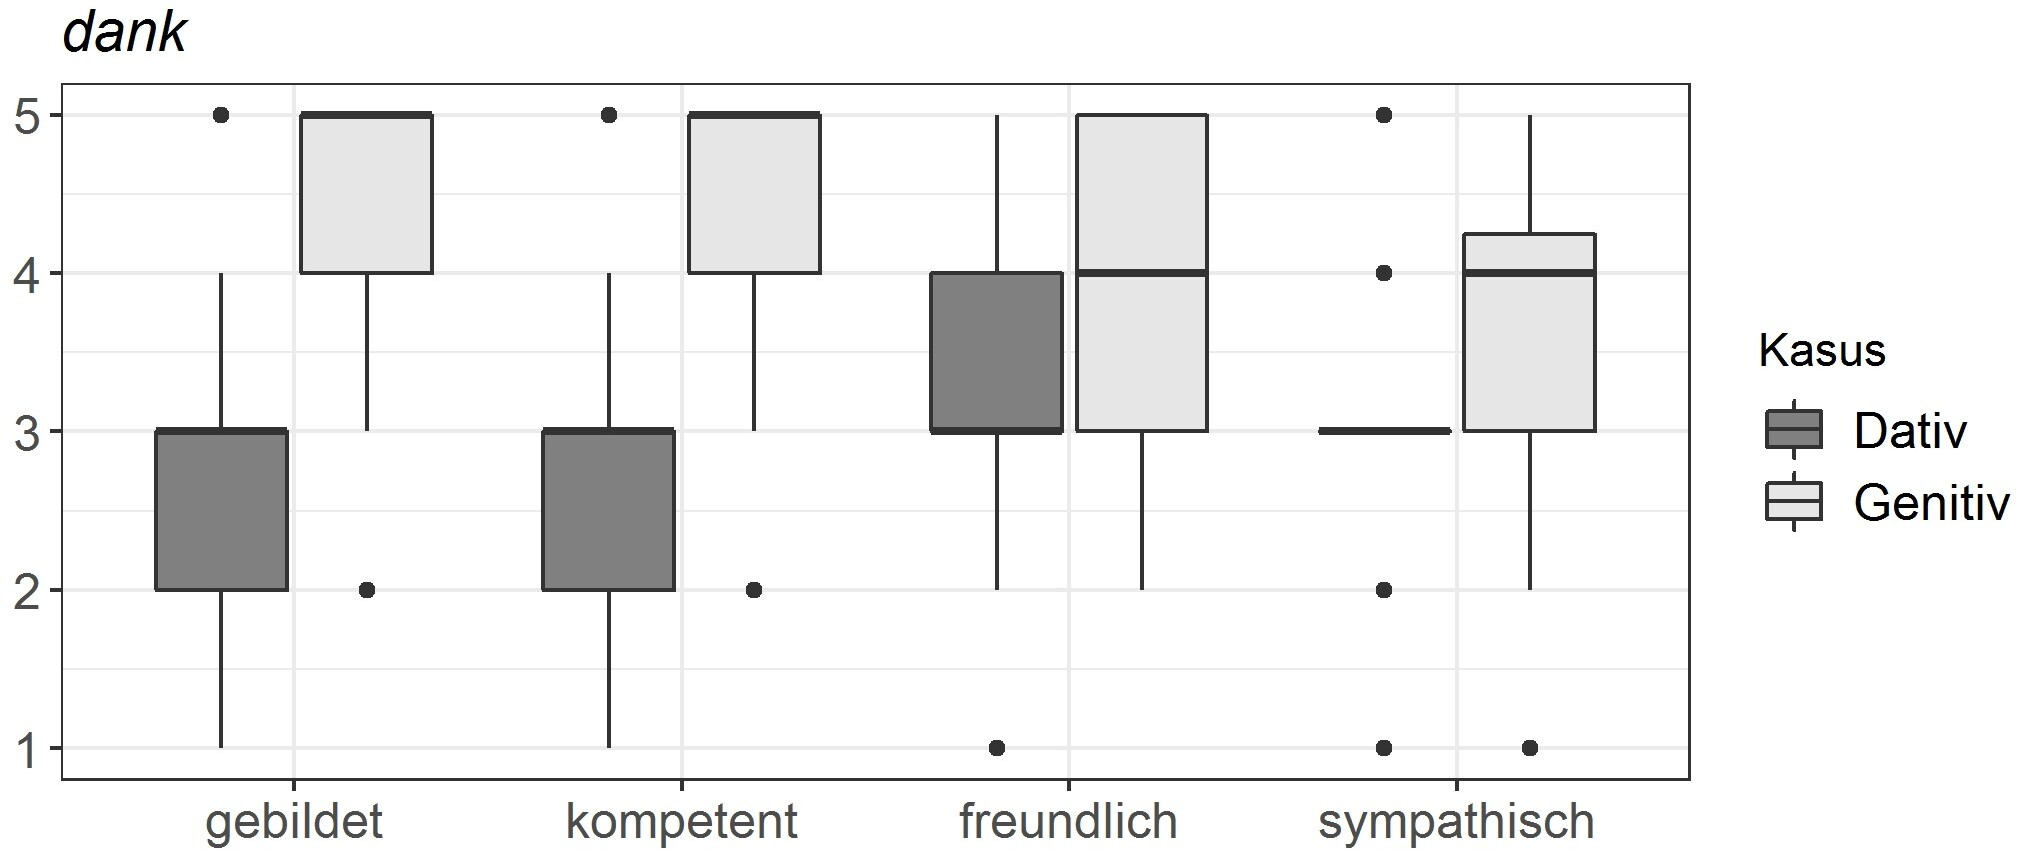
\includegraphics[width=\textwidth]{sdsdankBoxplots.jpg}
\caption{Bewertung der Rektionsvarianten von \dank}
\label{pic:sdsDank}
\end{figure}

Bei der Bewertung von \dank{} plus Genitiv als gebildet und kompetent scheint es außerdem eine hohe Einigkeit unter den Befragten zu geben, was sich darin zeigt, dass das untere Quartil jeweils bei 4 liegt. 
Der Großteil der Gruppe, die die Rektionsvarianten von \dank{} bewertete, hat in den Statuskategorien für die Genitivrektion also einen der beiden höchsten Werte gewählt: 
Auf der Skala für die Kategorie Bildung kreuzten insgesamt 87 von 96 Befragten 4 oder 5 an, auf der Skala für die Kategorie Kompetenz waren es 78 (s. \autoref{table:sdsdankAnh} im Anhang). 
Gleichzeitig wird die Genitivrektion bei \dank{} aber auch als sympathisch und freundlich eingestuft (Median jeweils 4). 
\object{Dank} plus Genitiv erzielt also sowohl in den Status- als auch in den Wärmekategorien hohe Werte. 

Bei der Dativrektion hingegen neigen die Befragten dazu, mittlere Werte anzukreuzen:
Alle Mediane für die Dativrektion bei \dank{} liegen bei 3. 
Besonders stark trifft dies auf die Wärmekategorie Sympathie zu: 
Der Median entspricht hier dem oberen und dem unteren Quartil, der Interquartilsabstand beträgt demnach 0. 
Im Falle der Kategorie Freundlichkeit entspricht der Median dem unteren Quartil, während er bei den Statuskategorien Bildung und Kompetenz dem oberen Quartil entspricht. 
Dies deutet darauf hin, dass die Dativrektion im Bereich der Wärmekategorien etwas positiver bewertet wird als im Bereich der Statuskategorien.

Bei der Präposition \gegenueber{} wird die Dativrektion gerade in den Statuskategorien Bildung und Kompetenz positiver bewertet als die Genitivrektion (s. \autoref{pic:sdsGegenueber}). 
Dies trifft insbesondere auf die Kategorie Bildung zu:
Während der Median für die Bewertung der Dativrektion bei 4 liegt, ist der mittlere Wert für die Bewertung der Genitivrektion 2. 
Auch im Bereich der Kompetenz wird die Dativrektion bei \gegenueber{} mit einem Median von 3 höher eingeschätzt als die Genitivrektion (m=2). 
\begin{figure}
\centering
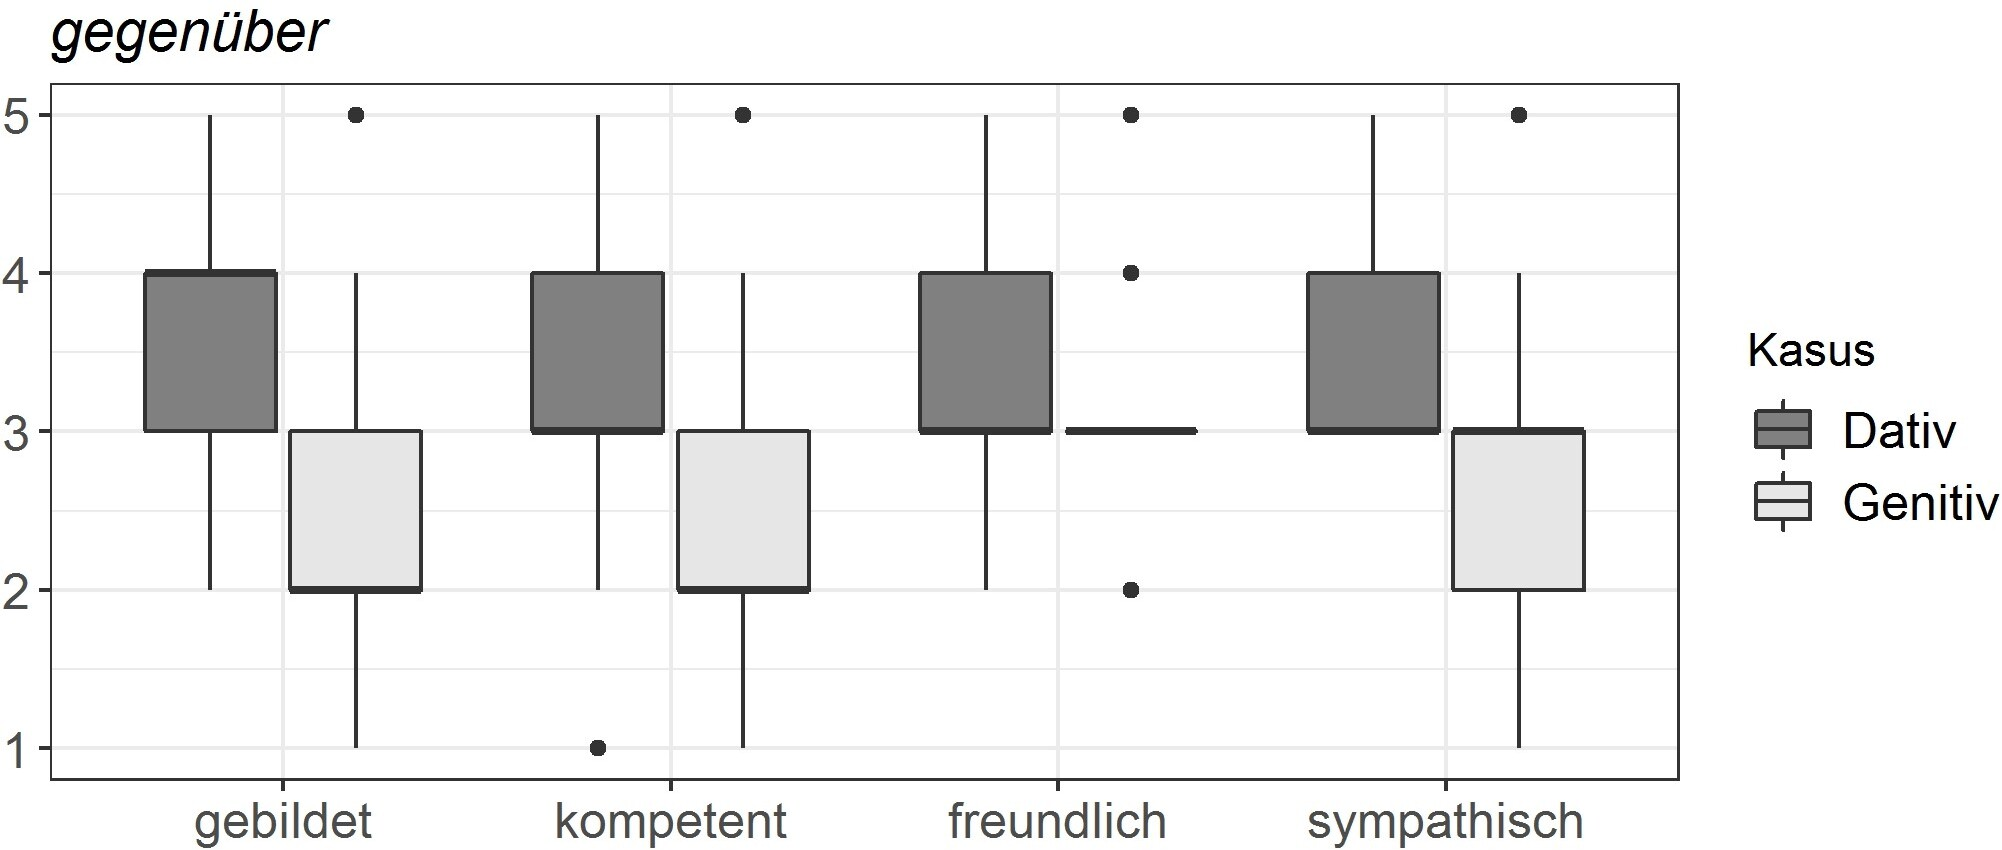
\includegraphics[width=\textwidth]{sdsgegenueberBoxplots.jpg}
\caption{Bewertung der Rektionsvarianten von \gegenueber}
\label{pic:sdsGegenueber}
\end{figure}

%In den Statuskategorien Bildung und Kompetenz scheint \gegenueber{} mit der Genitivrektion für die Befragten schwer einschätzbar zu sein: Die relativ  hohen Standardabweichungen von über 1,0 deuten hier darauf hin, dass die Einschätzungen recht unterschiedlich ausfallen. 
Für die Kategorien Freundlichkeit und Sympathie liegen die Mediane für alle Varianten bei 3. 
Auch hier werden bei den Dativvarianten aber häufiger Werte über 3 vergeben als bei den Genitivvarianten. 
Eine hohe Einigkeit herrscht offenbar darüber, dass \gegenueber{} mit dem Genitiv durchschnittlich freundlich klingt, hier beträgt der Interquartilsabstand 0.  
Bei der Bewertung der Sympathie von \gegenueber{} plus Dativ fällt zudem auf, dass die beiden niedrigsten Werte, 1 und 2, kein einziges Mal vergeben wurden. 
Die Dativrektion bei \gegenueber{} wird also von niemandem als unsympathisch empfunden.
Dies überrascht insofern wenig, als die Präposition noch kaum in ihrer Rektion schwankt und der Dativ der deutlich frequentere Kasus ist. %Änderung Anfang
Die Genitivrektion hingegen wird von einigen Befragten als wenig sympathisch beurteilt, sodass \gegenueber{} die einzige Präposition ist, bei der diese Rektionsvariante niedrige Werte in den Status- und Wärmekategorien erhält. %Änderung Ende

Insgesamt lässt sich bei allen Präpositionen erkennen, dass der Rektionskasus die Einschätzung der Freundlichkeit und Sympathie einer Person kaum beeinflusst.
Lediglich bei \dank{} unterscheiden sich die Mediane für Dativ und Genitiv bei diesen beiden Kategorien.  
Die folgende Aussage eines Befragten im freien Kommentar am Ende des Fragebogens bestätigt, dass die Kategorien Freundlichkeit und Sympathie nicht in das Bedeutungspotenzial der Rektionsvarianten fallen: 
\begin{exe}
\ex \object{Die Frage, ob eine Formulierung sympathisch ist oder nicht, finde ich schwierig, da der Tonfall und die Mimik bzw. Gestik hauptsächlich ausmacht, ob etwas sympathisch ist.} (Sozialversicherungsfachangestellter, 25)\footnote{Alle Kommentare aus dem Fragebogen werden genauso wiedergegeben, wie sie von den Befragten eingegeben wurden, also inklusive eventueller Tippfehler usw.}
\end{exe}
Anders als in vielen dialektologischen Studien zeigt sich bei den Rektionsvarianten also offenbar keine Differenzierung in dem Sinne, dass eine Variante in den Wärmekategorien besser bewertet würde, während die andere in den Statuskategorien höher eingeschätzt wird (\autoref{sec:Bewertungsgrundlage}).
Dies könnte daran liegen, dass Dialekte bzw. auch stark indexikalisch aufgeladene dialektale Varianten aufgrund ihres regionalen Bezugs ein höheres Identifikationspotenzial für Gruppen bieten als die hier abgefragten Rektionskasus.
% Änderung Anfang
Zudem könnte die hohe Bewertung beider Dimensionen für die Genitivvarianten von \wegen, \waehrend{} und \dank{} darauf hindeuten, dass diese Varianten dem Standard zugeschrieben werden und damit der Sprechergruppe, die als Referenz für alle gilt (s. dazu \autoref{sec:Bewertungsgrundlage}). %Änderung Ende

Zu der Bewertung der Rektionsvarianten auf den semantischen Differenzialen lässt sich insgesamt sagen, dass es eine starke Tendenz zur positiven Bewertung gibt. 
Dies zeigt sich etwa darin, dass die niedrigste Option auf der Bewertungsskala bei vielen Items von niemandem ausgewählt wurde. 
Der höchste Wert hingegen wurde bei allen Items vergeben -- außer im bereits angesprochenen Fall der Bewertung der Bildung bei \waehrend{} plus Dativ. 
Diese Tendenz zur positiven Bewertung kann als ein Effekt der sozialen Erwünschtheit verstanden werden (\autoref{sec:Methodologie}): 
Offenbar haben die Befragten Hemmungen, Personen aufgrund ihres Sprachgebrauchs negativ zu bewerten.
Darauf deutet auch diese Aussage eines Befragten im Kommentar am Ende des Fragebogens hin:
% \newpage 
\begin{exe}
\ex \object{Intelligenz/Kompetenz anhand von grammatikalischer Sicherheit einzuschätzen ist vielleicht noch machbar, aber ich halte es für schwierig, soziale Aspekte danach einzuschätzen, auch nicht so kluge Menschen können super lieb sein} (Student Ingenieurwissenschaften, 23)
\label{Bsp:Kommentarsds2}
\end{exe}
Die Äußerung präsupponiert, dass die Verwendung der Rektionsvarianten von der sprachlichen Sicherheit der SprachbenutzerInnen abhängt. 
Über diese Assoziation mit sprachlicher Sicherheit kann eine Variante auf einer höheren indexikalischen Ordnung geradezu ikonisch mit Eigenschaften wie Kompetenz oder Bildung verknüpft sein. 
Dies wird in einer weiteren Präsupposition der Äußerung in \autoref{Bsp:Kommentarsds2} ersichtlich, nämlich dass die Verwendung der Dativrketion darauf schließen lasse, jemand sei \object{nicht so klug}. 
Mit Eigenschaften wie Freundlichkeit oder Sympathie hingegen wird sprachliche Unsicherheit und damit auch die Dativrektion weniger stark in Verbindung gebracht. 
%Spielt hierfür vielleicht auch eine Rolle, dass nur ein Merkmal bewertet wird und nicht ein ganzes Register?

Der Kommentar in \autoref{Bsp:Kommentarsds2} zeigt bereits, dass es für eine umfassende Analyse der Indexikalität der Rektionskasus nicht ausreichend ist, Skalenwerte zu betrachten. 
Offene Fragen zu freien Assoziationen können noch sehr viel detailliertere Einblicke in die metapragmatische Bewertung der Varianten geben. 
Im folgenden Abschnitt wird die Auswertung solcher freien Assoziationen aus dem Fragebogen erläutert. 
\subsection{Überblick über die Assoziationskategorien}
\label{sec:ErgAssKat}
Wie oben bereits beschrieben, wurde je ca. 100 Befragten eine der vier Sekundärpräpositionen (\wegen, \waehrend, \dank{} oder \gegenueber) mit beiden Rektionsvarianten präsentiert (s. \autoref{table:Ass}). 
Zu jeder der beiden Rektionsvarianten wurden die Befragten nach freien Assoziationen gefragt, die sie als beliebig lange Antwort in ein Textfeld eintragen konnten. 
Aus diesem Design ergibt sich, dass insgesamt knapp unter 800 Antworten erhoben wurden (je zwei pro UntersuchungsteilnehmerIn). 
Diese wurden, wie in \autoref{sec:KategorisierungAss} beschrieben, inhaltsanalytisch in Kategorien gegliedert.
Dafür wurde mit der Software \citet{MAXQDA.19892018} gearbeitet. 
Das Kodierungshandbuch mit genauen Anweisungen für die Kategorisierung befindet sich im Anhang (\autoref{Anh:HandbuchAss}).
 
Da bereits die Assoziationskategorien Ergebnis einer ersten Analyse der freien Antworten sind, erfolgt hier einleitend eine Darstellung des Kategoriensystems. 
Diese gibt einen Überblick über die Bandbreite der Assoziationen, auf die in den darauffolgenden Abschnitten im Einzelnen eingegangen wird. 

Das Kategoriensystem besteht aus 16 Oberkategorien mit bis zu zwei Ebenen von Unterkategorien. 
Bspw. verfügt die Oberkategorie \glqq Personentypus\grqq{} über die Unterkategorie \glqq Bildung\grqq{} (erste Ebene), die wiederum die Unterkategorie \glqq gebildet\grqq{} aufweist (zweite Ebene). 
Um den Zusammenhang solcher Ober- und Unterkategorien anzuzeigen, wird hier folgende Notation verwendet: \glqq Personentypus > Bildung > gebildet\grqq.

In \autoref{table:KatsysAss} sind die 16 Oberkategorien sowie die erste Ebene der Unterkategorien aufgeführt. 
%Einige Oberkategorien verfügen über mehr als eine Ebene von Unterkategorien, etwa die eben genannte Oberkategorie \glqq Person\grqq{} oder die Oberkategorie \glqq Ästhetik\grqq, bei der sich bspw. die Unterkategorie \glqq ästhetisch\grqq{} noch einmal aufteilt in \glqq elegant/gehoben\grqq{} und \glqq gut/schön\grqq. 
Eventuell vorhandene weitere Unterkategorisierungen werden in den einzelnen Abschnitten zu den jeweiligen Oberkategorien beschrieben.
\autoref{table:Ass} zeigt neben den ersten beiden Kategorienebenen, wie viele Kodierungseinheiten jeder Oberkategorie zugewiesen wurden. 
Auf diese Verteilung wird später noch genauer eingegangen. 

\begin{table}
\small
\begin{tabular}{ll|r}
\multicolumn{2}{l|}{Oberkategorien und Unterkategorien} & Anzahl Kodierungen \\ \hline
\multicolumn{2}{l|}{Korrektheit} & 282 \\ %\hline
\textbf{} & - falsch &  \\ 
\textbf{} & - richtig &  \\ \hline
\multicolumn{2}{l|}{Zweifel} & 8 \\ \hline
\multicolumn{2}{l|}{Gleichgültigkeit} & 4 \\ \hline\multicolumn{2}{l|}{Herleitung} & 9 \\ \hline
\multicolumn{2}{l|}{Bedeutung und Verständlichkeit} & 10 \\ \hline
\multicolumn{2}{l|}{eigener Sprachgebrauch} & 23 \\ %\hline
\textbf{} & - entspricht eigenem Gebrauch nicht &  \\ 
\textbf{} & - entspricht eigenem Gebrauch &  \\ \hline
\multicolumn{2}{l|}{Sprachwandel} & 31 \\ %\hline
\textbf{} & - natürlicher Wandel &  \\ 
\textbf{} & - Sprachverfall &  \\ \hline
\multicolumn{2}{l|}{Formalität} & 89 \\ %\hline
\textbf{} & - informell &  \\ 
\textbf{} & - formell &  \\ \hline
\multicolumn{2}{l|}{Medium} & 45 \\ %\hline
\textbf{} & - schriftlich &  \\ 
\textbf{} & - mündlich &  \\ \hline
\multicolumn{2}{l|}{Varietät} & 76 \\ %\hline
\textbf{} & - Standard &  \\ 
\textbf{} & - Regionalsprache/Dialekt &  \\ 
\textbf{} & - Umgangs-/Alltagssprache &  \\ \hline
\multicolumn{2}{l|}{Ästhetik} & 195 \\ %\hline
\textbf{} & - auffällig/ungewohnt &  \\ 
\textbf{} & - unauffällig/normal &  \\ 
\textbf{} & - nicht ästhetisch &  \\ 
\textbf{} & - ästhetisch &  \\ 
\textbf{} & - simpel &  \\ \hline
\multicolumn{2}{l|}{Personentypus} & 191 \\ %\hline
\textbf{} & - Vertrautheit &  \\ 
\textbf{} & - Charakter &  \\ 
\textbf{} & - soziale Gruppe &  \\ 
\textbf{} & - Bildung &  \\ 
\textbf{} & - Sprachkompetenz &  \\ \hline
\multicolumn{2}{l|}{Stellung} & 7 \\ \hline
\multicolumn{2}{l|}{nicht relevant} & 27 \\ \hline
\multicolumn{2}{l|}{keine Assoziation} & 60 \\ \hline
\multicolumn{2}{l|}{nicht entscheidbar} & 23 \\ 
\end{tabular}
\caption{Oberkategorien und erste Ebene der Unterkategorien für die Inhaltsanalyse der freien Assoziationen}
\label{table:KatsysAss}
%\end{small}
\end{table}
%\begin{figure}[htbp]
%
\includegraphics[scale=1]{KategoriensystemAsssw.png}
%\caption{Oberkategorien und erste Ebene der Unterkategorien für die Inhaltsanalyse der freien Assoziationen}
%\label{pic:KatsysAss}
%\end{figure}  Als Kodierungseinheit diente jeweils eine komplette Äußerung, also eine Antwort zu einer Variante.
Ein wichtiges Prinzip der Kodierung ist, dass eine Kodierungseinheit mehreren Kategorien zugeordnet werden konnte. 
Durch diese Möglichkeit der Mehrfachkodierung kommt es zu einer Gesamtzahl von 1080 Kodierungen. 
Die folgende Antwort zu \dank{} mit der Dativrektion bspw. wurde mit \glqq Formalität > informell\grqq, \glqq Medium > mündlich\grqq{} und \glqq Personentypus > Vertrautheit/Nähe\grqq{} kodiert: 
\begin{exe}
\ex \object{informelle Unterhaltung, mit vertrauten Personen, z. B. Familie, enge Freunde, befreundete Arbeitskollegen in informeller Situation}\footnote{Da die Metadaten für die Erläuterung der Kategorien nicht relevant sind, werden sie bei den in diesem Abschnitt zitierten Kommentaren nicht aufgeführt.}
\end{exe}
Wenn in einer Antwort allerdings mehrfach auf die gleiche Kategorie Bezug genommen wird, so findet sich die Antwort dennoch nur einmal in dieser Kategorie. 
Bspw. verweist die Aussage \object{locker, informell} sowohl mit \object{locker} als auch mit \object{informell} auf die Informalität von \dank{} mit dem Dativ. 
Dennoch wird die Antwort nur einmal als \glqq Formalität > informell\grqq{} kategorisiert.

Recht zahlreich finden sich Antworten, die auf die sprachliche Richtigkeit der präsentierten Variante abzielen. 
Insgesamt 282 Antworten wurden in der Oberkategorie \glqq Korrektheit\grqq{} kodiert, die damit die frequenteste Kategorie ist. 
Sie weist lediglich zwei Unterkategorien auf, nämlich \glqq richtig\grqq{} und \glqq falsch\grqq. 
Hier finden sich etwa Antworten wie \object{der Genitiv ist richtig}. 

Die Oberkategorie \glqq Zweifel\grqq{} beinhaltet Antworten, die sprachliche Zweifel ausdrücken, wie etwa diese Äußerung, die sich auf \gegenueber{} bezieht: 
\begin{exe}
\ex \object{Je öfter ich es lese, desto weniger weiß ich ob es richtig ist -- spontan bin ich unschlüssig. Ich hätte weder 1 noch 2 formuliert}. 
\end{exe}
Wenige Befragte äußern, dass sie beide Varianten gleichermaßen akzeptieren. 
Antworten wie die folgende zu \dank{} finden sich in der hierfür angelegten Kategorie \glqq Gleichgültigkeit\grqq.
\begin{exe}
\ex \object{bei dank dem/des ist mir das egal}
\end{exe}
Diese Oberkategorie weist keine Unterkategorien auf.

In den Assoziationen der Oberkategorie \glqq Herleitung\grqq{} versuchen Befragte, sprachlich zu begründen, inwiefern eine Form korrekt ist, wie etwa in folgender Antwort: 
\begin{exe}
\ex \object{Es heißt weswegen? nicht wemwegen?}
\end{exe}

In die Kategorie \glqq Bedeutung und Verständlichkeit\grqq{} fallen Antworten, die etwa darauf hinweisen, dass ein Beispiel gut oder schlecht verständlich ist oder eine bestimmte Lesart im Vordergrund steht. 
So etwa diese Aussage zu \gegenueber{} mit dem Dativ: 
\begin{exe}
\ex \object{Ich verstehe die Aussage sofort, mir fällt nichts besonderes dazu ein.}
\end{exe}
Die Kategorie \glqq Bedeutung und Verständlichkeit\grqq{} weist keine Unterkategorien auf, wie in \autoref{table:KatsysAss} zu erkennen ist.
 
%\autoref{sec:ErgAssKorrektheit} geht insbesondere auf die Assoziationen mit Korrektheit ein, da diese besonders zahlreich sind, berücksichtigt aber auch die Kategorien \glqq Herleitung\grqq, \glqq Zweifel\grqq{} und \glqq Gleichgültigkeit\grqq.
Unter der Oberkategorie \glqq eigener Sprachgebrauch\grqq{} wurden Antworten kodiert, die eine Variante mit dem eigenen Sprachgebrauch in Verbindung bringen, indem sie entweder aussagen, dass eine Variante der eigenen Verwendung entspricht oder dass eine Variante der eigenen Verwendung nicht entspricht. 
So etwa diese Antwort zu \dank{} mit der Genitivrektion: 
\begin{exe}
\ex \object{Diese Variante würde ich verwenden }
\end{exe}
In die Oberkategorie \glqq Sprachwandel\grqq{} fallen auf der einen Seite Assoziationen, die auf den natürlichen Wandel der Sprache Bezug nehmen, auf der anderen Seite solche, die eine negative Einstellung gegenüber dem Sprachwandel erkennen lassen. 
Letztere Kategorie beinhaltet vor allem die häufig getätigte Aussage \object{der Dativ ist dem Genitiv sein Tod} (vgl. \autoref{sec:IndexikalitaetRektionskasushistorisch}).

Den Oberkategorien \glqq Formalität\grqq, \glqq Medium\grqq{} und \glqq Varietät\grqq{} ist gemein, dass sie sich alle mit der Angemessenheit der Variante in bestimmten Kontexten oder der Evozierung dieser Kontexte durch die Varianten beschäftigen. 
Die Assoziationen zur Formalität lassen sich dabei in Zuschreibungen zu einem informellen Register und Zuschreibung zu einem formellen Register unterteilen. 
Darunter fallen bspw. Aussagen, die Varianten als \object{locker} oder \object{förmlich} bezeichnen. 
In die Oberkategorie \glqq Medium\grqq{} fallen Antworten, die eine Variante mit phonischer oder graphischer Realisierung in Verbindung bringen. Ein Beispiel ist diese Äußerung zu \dank{} mit der Dativrektion, die zusätzlich der Kategorie \glqq eigner Sprachgebrauch > entspricht eigenem Gebrauch\grqq{} zugeordnet wurde: 
\begin{exe}
\ex \object{Würde ich im mündlichen Sprachgebrauch verwenden}
\end{exe}
Unter \glqq Varietät\grqq{} finden sich Zuschreibungen zur Standardsprache und Beschreibungen der Variante als umgangs- oder alltagssprachlich sowie Assoziationen mit dem Sprachgebrauch einer bestimmten Region oder mit dialektalem Sprachgebrauch allgemein, wie im folgenden Beispiel:
\begin{exe}
\ex \object{Es hört sich sprachlich falsch an, kann aber auch aus einem Dialekt stammen, den ich nicht kenne.}
\end{exe}
Knapp ein Viertel der Antworten bezieht sich auf ästhetische Dimensionen einer Variante, wie etwa die folgenden: 
\begin{exe}
\ex \object{Klingt holprig} \label{Bsp:holperig}
\ex \object{Klingt komisch} \label{Bsp:komisch}
\end{exe}
Diese finden sich unter der Oberkategorie \glqq Ästhetik\grqq. 
Zum einen fallen hierunter Aussagen, die eine Variante entweder als unschön bezeichnen, wie in \autoref{Bsp:holperig}, oder aber als schön (\glqq nicht ästhetisch\grqq{} bzw. \glqq ästhetisch\grqq), zum anderen Aussagen über die Auffälligkeit oder Unauffälligkeit der Varianten, wie \autoref{Bsp:komisch} (\glqq auffällig/ungewohnt\grqq{} bzw. \glqq unauffällig/normal\grqq). 
Daneben finden sich unter der Oberkategorie \glqq Ästhetik\grqq{} außerdem einige wenige Antworten, die eine Variante als \glqq simpel\grqq{} beschreiben, z.\,B.:
\begin{exe}
\ex \object{Einfachere Sprachform} 
%(Pflegedienstleiterin, 37, zu \dank{} mit dem Dativ)
\end{exe}

In 191 Antworten finden sich Assoziationen, die mit der Produzentin oder dem Empfänger einer Variante zusammenhängen, sich also auf Eigenschaften von Personen beziehen, wie etwa das folgende Beispiel zu \dank{} mit dem Genitiv: 
\begin{exe}
\ex \object{Arroganz, Selbstgefälligkeit, gebildet} \label{Bsp:Arroganz}
\end{exe}
Unter personenbezogene Assoziationen fallen zunächst Zuschreibungen einer Variante zu bestimmten Charaktereigenschaften sowie Zuschreibungen zu sozialen Gruppen, wie etwa AkademikerInnen.
Eine eigene Unterkategorie bilden dabei Assoziationen mit niedriger oder hoher Bildung, da diese besonders zahlreich sind (\autoref{sec:ErgAssPersonen}). 
In \autoref{Bsp:Arroganz} etwa wird sowohl auf den Charakter der sich äußernden Person Bezug genommen als auch auf deren Bildung, weshalb diese Äußerung in beiden Unterkategorien kodiert ist. 
Daneben finden sich Antworten, die sich auf die Vertrautheit der InteraktionspartnerInnen beziehen. 
Außerdem nehmen einige Kommentare Bezug auf die Sprachkompetenz von Personen, die mit der Verwendung einer präsentierten Variante assoziiert werden. 

In eine weitere Kategorie fallen Assoziationen, die sich nicht auf die Rektion, sondern auf die Stellung der Präposition beziehen. 
Diese finden sich ausschließlich zur Präposition \gegenueber, bei der einige Befragte die Poststellung präferiert hätten.
Auch die Kategorie \glqq Stellung\grqq{} kommt ohne eine weitere Untergliederung aus. 

In der Kategorie \glqq nicht relevant\grqq{} wurden Antworten gesammelt, die lediglich Assoziationen enthalten, die erkennbar nicht mit der Rektion der Varianten zusammenhängen und sich meist auf den Inhalt der Beispielsätze beziehen. 
Etwa wenn ein Befragter zum Beispiel \object{Sie hat es gegenüber dem Lehrer nicht erwähnt} schreibt: 
\begin{exe}
\ex \object{Sie hat dem Lehrer etwas verschwiegen}
\end{exe}
Wenn in einer Antwort keine Assoziationen erkennbar sind, wurde die Kategorie \glqq keine Assoziation\grqq{} vergeben. 
Hierunter fallen bspw. Antworten, in denen Befragte lediglich einen Strich eingetragen oder etwas wie \object{nichts} geschrieben haben. 
Bei einigen Antworten schließlich war auch nach der gemeinsamen Durchsicht durch die drei Kodiererinnen nicht entscheidbar, in welcher Kategorie sie zu kodieren wären. 
Diese insgesamt 23 Antworten wurden als \glqq nicht entscheidbar\grqq{} gewertet. 
Dazu gehören etwa die folgenden:
\begin{exe}
\ex \object{Wer oder was, wessen, wem, wen oder was???}
\ex \object{?}
\end{exe} 
Die drei Oberkategorien, \glqq nicht relevant\grqq, \glqq keine Assoziation\grqq{} und \glqq nicht entscheidbar\grqq, sind von dem oben beschriebenem Prinzip der Mehrfachkodierung ausgeschlossen. 
Das heißt, diese Kategorien wurden nur dann vergeben, wenn eine Kodierungseinheit keine weiteren Assoziationen enthielt.
Die Antwort \object{gar keine, würde mir nicht auffallen, da richtig} bspw. wurde nicht in \glqq keine Assoziation\grqq{} kodiert, da entgegen der ersten Aussage in der Antwort Assoziationen zur Ästhetik (\glqq unauffällig/normal\grqq) und zur Korrektheit (\glqq richtig\grqq) geäußert werden.  
Dieses Vorgehen ermöglicht es, Äußerungen, die für die weitere Analyse nicht herangezogen werden können, da sie keine (relevanten) oder lediglich unklare Assoziationen enthalten, leicht zu identifizieren. 

In \autoref{pic:OKatAss2} ist zusammenfassend dargestellt, wie sich die insgesamt 1080 Kodierungen auf die hier beschriebenen 16 Oberkategorien verteilen. 
Die Kategorien sind entsprechend der Anzahl der ihnen zugeordneten Assoziationen geordnet, sodass ersichtlich wird, welche Aspekte für die Befragten besonders relevant sind.
\begin{figure}
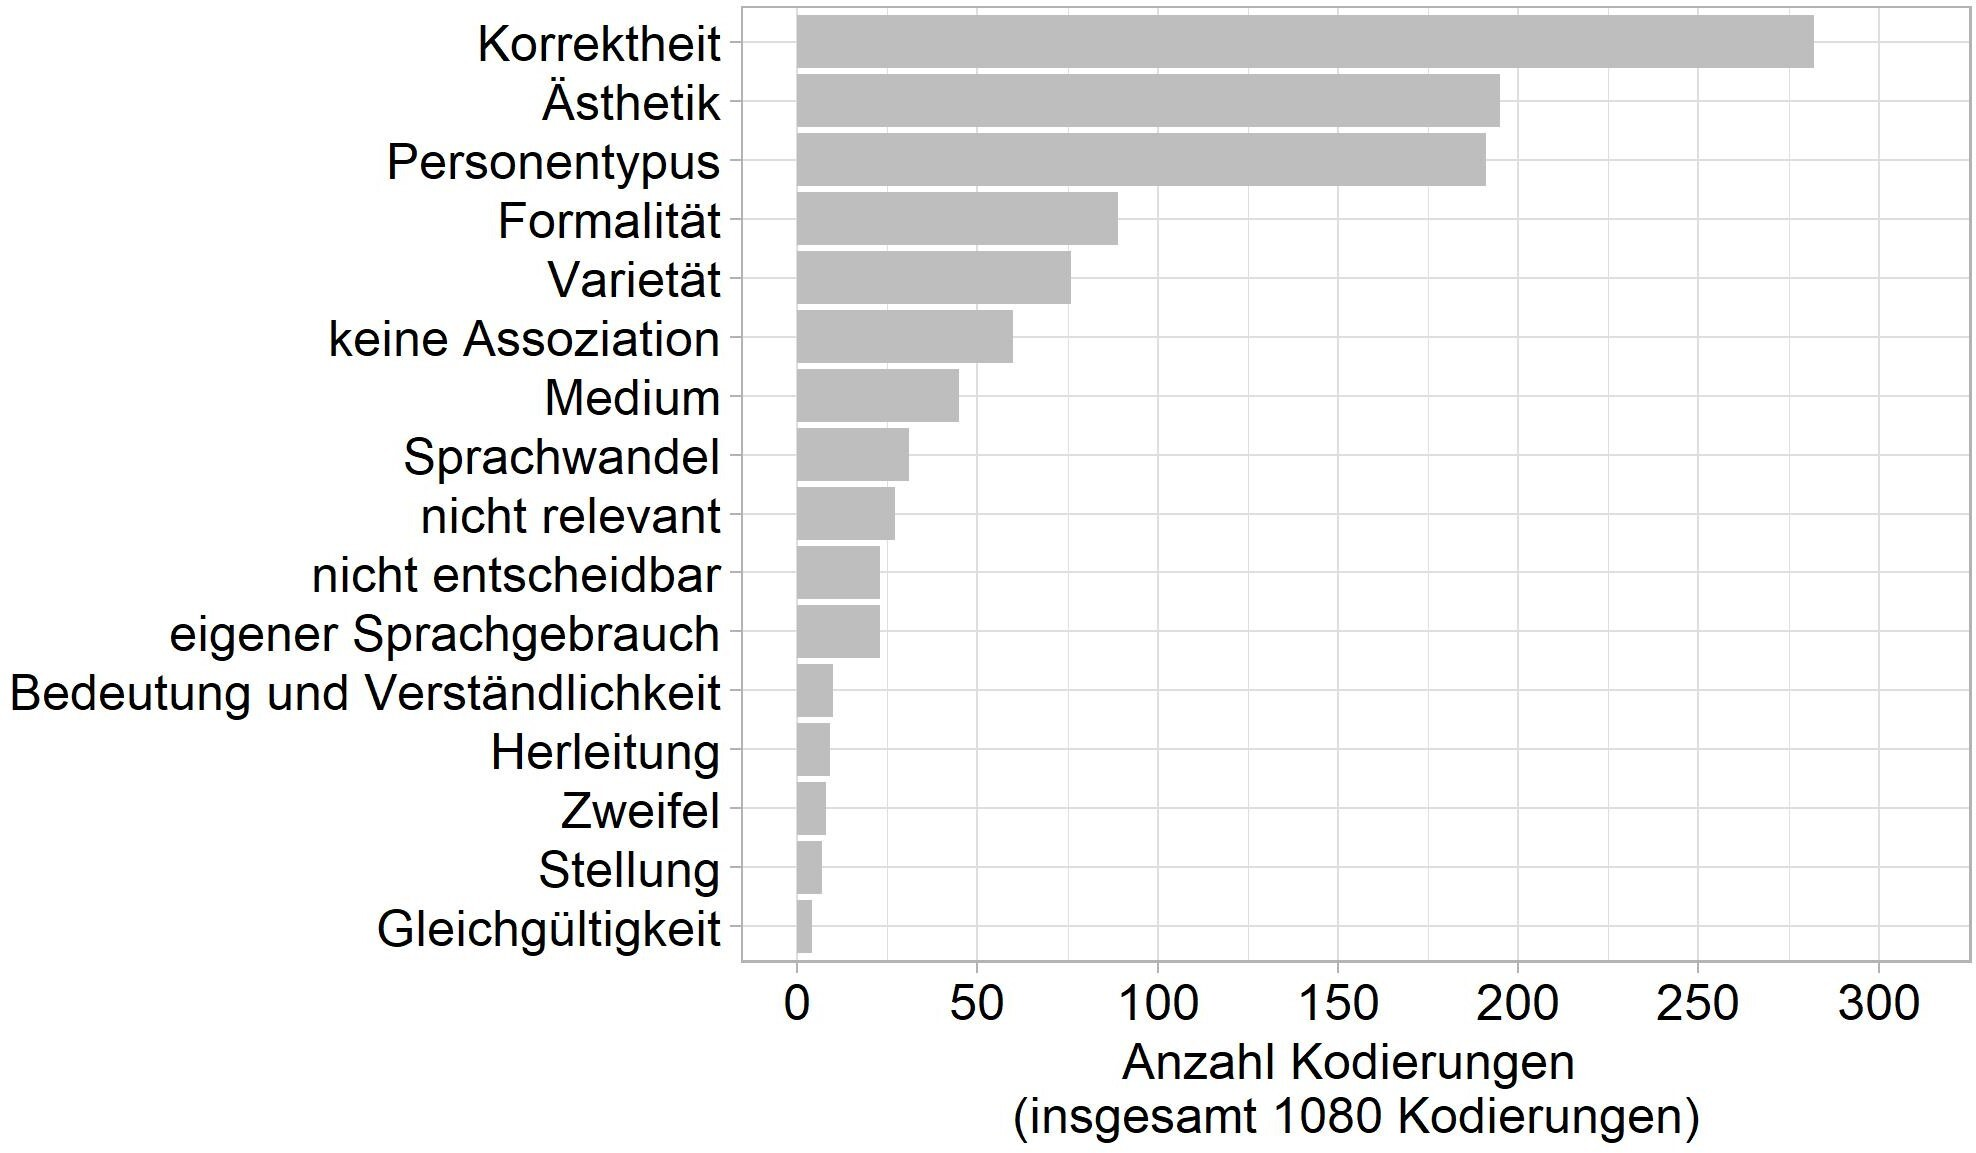
\includegraphics[width=\textwidth]{OKatAss.jpg}
\caption{Anzahl der Kodierungen in den 16 Oberkategorien}
\label{pic:OKatAss2}
\end{figure}
Demnach wird in den Antworten insbesondere auf die Korrektheit der Varianten sehr häufig verwiesen: Diese Kategorie macht ca. ein Viertel aller Kodierungen aus. 
Assoziationen mit ästhetischen Eigenschaften sowie mit Personentypen spielen ebenfalls eine wichtige Rolle. 
Auch Assoziationen mit Formalität, Varietät oder Medium sind recht zahlreich: 
89 Assoziationen betreffen die Formalität einer Variante, 45 das Medium und 76 einen varietätslinguistischen Aspekt. 
Die Oberkategorie \glqq Sprachwandel\grqq{} ist mit 31 Kodierungen ebenfalls erwähnenswert. 
Auf diese in den Assoziationen stark vertretenen Oberkategorien wird in den folgenden Abschnitten %Änderung Anfang
in der Reihenfolge ihrer Häufigkeit %Änderung Ende 
detaillierter eingegangen. 

Auch der Fall, dass keine Assoziation geäußert wurde, ist relativ häufig:
Insgesamt 60 Antworten enthalten keine Assoziationen. 
Berücksichtigt man zusätzlich Antworten der Kategorie \glqq nicht relevant\grqq{}, so ergibt dies 87 Antworten, in denen sich keinerlei Assoziation zu einem der Rektionskasus ausmachen lässt. 
Diese Beobachtung unterstreicht einen Vorteil der Erhebung freier Assoziationen gegenüber der Verwendung semantischer Differenziale: 
Während Befragte im Falle der semantischen Differenziale gezwungen sind, ein Kreuz innerhalb bereits vorgegebener Kategorien zu setzen, gibt die Frage nach freien Assoziationen den Blick frei auf Fälle, in denen Befragte mit einer Variante keine soziale Bedeutung verbinden.  

Im Anschluss an die Kategorisierung der Assoziationen wurden in MAXQDA zusätzlich die Metadaten Altersgruppe und Gender kodiert, um leichter auf diese Informationen über die Befragten zugreifen zu können. 
Jede Kodierungseinheit, also jede Antwort, verfügt daher mindestens über drei Kodierungen: Altersgruppe, Gender und mindestens eine inhaltliche Kategorie. 
\autoref{pic:ScreenshotMAXQDA} zeigt zur Veranschaulichung ein Beispiel in einem Screenshot aus MAXQDA. 
Links neben der Tabelle mit den Befragungsdaten erscheinen die vergebenen Kategorien. 
Neben der Kodierung in \glqq Korrektheit > richtig\grqq{} sind zusätzlich die Kodierungen der Metadaten zu sehen: \glqq Gender > männlich\grqq{} und \glqq Altersgruppe > 26--35\grqq.
%Falls das bunt bleibt, kurz auf die Farben eingehen! 

\begin{figure}
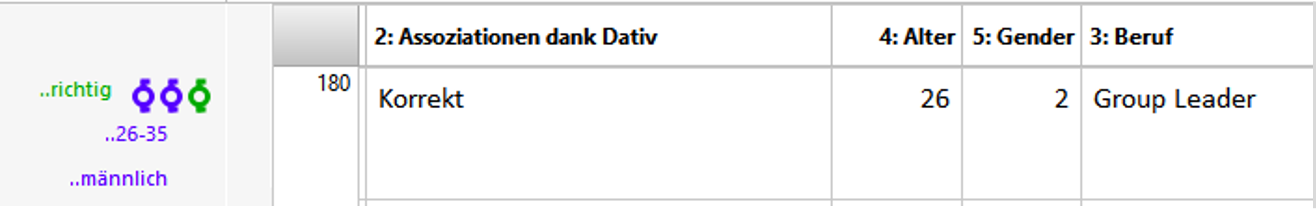
\includegraphics[width=\textwidth]{ScreenshotMAXQDAneu.png}
\caption{Screenshot aus MAXQDA: Darstellung der Kodierungen}
\label{pic:ScreenshotMAXQDA}
\end{figure}
\subsection{Assoziationen mit Korrektheit}
\label{sec:ErgAssKorrektheit}
% Korrektheit / Standardsprachideologie
Die häufigste Assoziation der Befragten ist die Zuordnung der präsentierten Variante zu den Kategorien \glqq richtig\grqq{} oder \glqq falsch\grqq. 
282 Antworten enthalten eine Assoziation zu dieser Kategorie. 
In der hohen Frequenz dieser Assoziation zeigt sich bereits die Relevanz der Standardsprachideologie und der damit verbundenen Annahme, es gebe stets nur eine korrekte Variante (\autoref{sec:Einheitlichkeit}). 
Offenbar führt die Konfrontation mit zwei Rektionsvarianten bei sehr vielen Befragten zu dem Bedürfnis, Richtig von Falsch zu unterscheiden. 
Welche Varianten sie dabei als richtig bezeichnen und welche als falsch, zeigt \autoref{pic:AssKorrektheit}. 

\begin{figure}
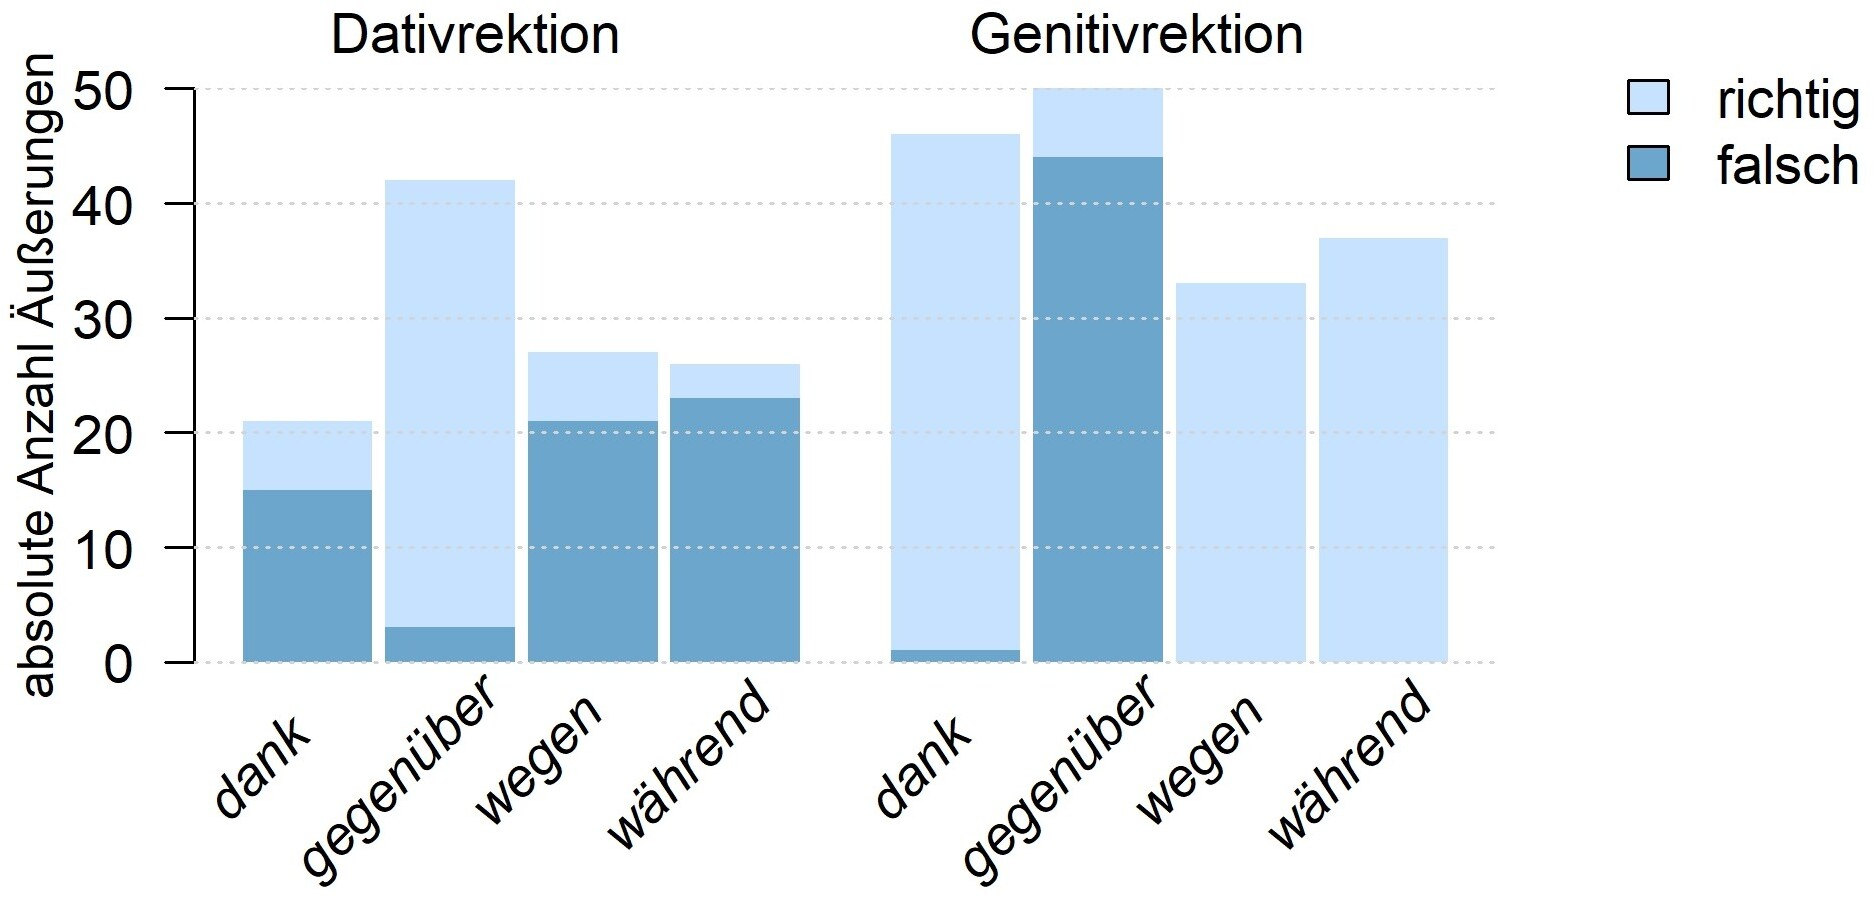
\includegraphics[width=\textwidth]{AssKorrektheit.jpg}
\caption{Verteilung der Assoziationen der Oberkategorie \glqq Korrektheit\grqq}
\label{pic:AssKorrektheit}
\end{figure}
Sowohl bei den ursprünglichen Genitivpräpositionen \wegen{} und \waehrend{} als auch bei der ursprünglichen Dativpräposition \dank{} überwiegen die Antworten, in denen die Dativrektion als falsch bezeichnet wird. 
Insgesamt finden sich 59 Äußerungen, die die Dativrektion als inkorrekt ansehen (für die genauen Zahlen s. auch \autoref{table:richtigfalschAnh} im Anhang). 
Die Genitivrektion wird bei \wegen, \waehrend{} und \dank{} beinahe ausschließlich als richtig angesehen: 
In insgesamt 116 Einstellungsäußerungen zu einer dieser drei Präpositionen mit dem Genitiv wird die Variante 115-mal als richtig bezeichnet.
Lediglich einmal bei \dank{} wird der Genitiv als falsch bezeichnet, allerdings mit dem Hinweis, dass \dank{} plus Genitiv zunächst richtig erscheine: 
\begin{exe}
\ex \object{Klingt richtig und vor allem bemüht richtig, ist aber falsch. Eselsbrücke: dank dir und nicht dank deiner} (Hotelrezeptionistin, 30, zu \dank{} mit dem Genitiv)\label{Bsp:bemueht}
\end{exe}
Die Aussage, der Genitiv klinge hier zwar korrekt, sei es in diesem Fall aber nicht, zeigt, wie stark der Genitiv mit Korrektheit in Verbindung gebracht wird.
Wird die Dativrektion als korrekte Variante bezeichnet, erscheint dies wie eine Ausnahme. 

Anders verhält es sich bei der Präposition \gegenueber{}: 
Hier wird die Genitivrektion, die noch sehr infrequent ist, von vielen als falsch empfunden.
Nur sechs Antworten bezeichnen die Genitivrektion bei \gegenueber{} als richtig. 
Interessant ist, dass es zu \gegenueber{} im Vergleich mit den anderen Präpositionen besonders viele Einstellungsäußerungen gibt, die auf die Korrektheit der Varianten Bezug nehmen. 
Dies kann ein erster Hinweis darauf sein, dass die Variation bei dieser Präposition (noch) keine starken anderen Assoziationen hervorruft, also kaum indexikalisch aufgeladen ist. 
%Darauf wird in \autoref{sec:Felder} näher eingegangen.

Bei einer näheren Betrachtung der Antworten in der Kategorie \glqq Korrektheit\grqq{} fällt auf, dass die Korrektheit unterschiedlich legitimiert wird: 
Während einige Antworten ein persönliches Korrektheitsempfinden anführen (\autoref{Bsp:irgendwiefalsch} und \autoref{Bsp:erscheintmirnichtrichtig}), werden die präsentierten Varianten in anderen Antworten kategorisch als falsch oder richtig dargestellt (\autoref{Bsp:falscherArtikel} und \autoref{Bsp:gehtdoch}). 
\begin{exe}
\ex \object{Klingt irgendwie falsch} (Postbeamtin, 53, zu \dank{} mit dem Dativ) \label{Bsp:irgendwiefalsch}
\ex \object{Erscheint mir nicht richtig, da der falsche Artikel verwendet wird.} (Biologiedoktorandin, 29, zu \dank{} mit dem Dativ) \label{Bsp:erscheintmirnichtrichtig}
\ex \object{Falscher Artikel} (Biologiestudent, 24, zu \dank{} mit dem Dativ) \label{Bsp:falscherArtikel}
\ex \object{Geht doch, richtig!} (Abteilungsleiterin, 51, zu \dank{} mit dem Genitiv) \label{Bsp:gehtdoch}
\end{exe}
Außerdem machen Antworten, in denen eine Variante als falsch bezeichnet wird, teilweise eine Einschränkung, indem sie einräumen, eine Variante sei zwar falsch, aber dennoch akzeptabel oder gebräuchlich.
So schreibt eine 19-jährige Psychologiestudentin zu \waehrend{} mit dem Dativ:
\begin{exe}
\ex \object{Falsch aber umgangssprachlich verbreitet und ok} (Psychologiestudentin, 19, zu \waehrend{} mit dem Dativ) \label{Bsp:falschumgangssprachlich}
\end{exe}
Hier zeigt sich die Annahme, dass Richtig und Falsch in der Sprache starre Kategorien sind, die unabhängig vom Sprachgebrauch feststehen. 
Als richtig scheint dabei die Variante empfunden zu werden, die als standardsprachlich registriert ist. 
Zu einem anderen Schluss kommt ein 26-jähriger Doktorand in seiner Äußerung zu \dank{} mit dem Dativ: 
\begin{exe}
\ex \object{Auch richtig, aber eher weniger im akademischen Kontext -> privat} (Geschichtsdoktorand, 26, zu \dank{} mit dem Dativ)
\end{exe}
Auch hier wird eine Unterscheidung zwischen sprachlicher Korrektheit und sprachlicher Angemessenheit getroffen. 
Jedoch wird der thematisierten Variante nicht nur eine eingeschränkte Angemessenheit, sondern auch eine eingeschränkte Korrektheit zugesprochen. 
Auf die Zusammenhänge zwischen Korrektheit und Angemessenheit wird in der Analyse der Ergebnisse des Akzeptabilitätstests (\autoref{sec:ErgAkzallg}) zurückzukommen sein. 

118 der 282 Äußerungen in der Kategorie \glqq Korrektheit\grqq{} wurden zusätzlich einer oder mehreren weiteren Kategorien zugeordnet, beziehen sich also nicht ausschließlich auf die Korrektheit der Variante, sondern daneben auf weitere Assoziationsbereiche. 
Besonders häufig (50-mal) werden Äußerungen zur Korrektheit etwa mit Assoziationen zur Ästhetik einer Variante kombiniert. 
\begin{exe}
\ex \object{klingt korrekt, eleganter bzw. flüssiger} (Wissenschaftliche Mitarbeiterin, 27, zu \dank{} mit dem Genitiv)
\end{exe} 
In diesem Beispiel wird zunächst lediglich ausgesagt, dass \dank{} mit der Genitivrektion korrekt erscheint, ohne dass die Variante mit der Dativrektion dabei als inkorrekt dargestellt wird. 
Die Komparativformen \object{eleganter} und \object{flüssiger} können aber als Vergleich mit der Dativrektion interpretiert werden, da beide Varianten im Fragebogen in direkter Opposition zueinander präsentiert werden. 
Hier wird also gewissermaßen für die Genitivvariante argumentiert, indem gesagt wird, dass diese nicht nur die Voraussetzung erfüllt, korrekt zu sein, sondern darüber hinaus ästhetischer erscheint als die Dativvariante. 

Im folgenden Beispiel wird \waehrend{} plus Dativ nicht nur als inkorrekt und unästhetisch bezeichnet, sondern außerdem mit ungebildeten SprecherInnen in Verbindung gebracht: 
\begin{exe}
\ex \object{Verkehrt, unschön, hohle Birne} (Jurastudentin, 25, zu \waehrend{} mit dem Dativ) \label{Bsp:hohleBirne}
\end{exe}
Solche Antworten, in denen Assoziationen zur Korrektheit einer Variante mit Assoziationen zu Personen kombiniert sind, finden sich in den Daten insgesamt 30-mal. 
47-mal werden Aussagen über die Korrektheit mit Aussagen zur Formalität, dem Medium oder der Varietät verbunden, wie etwa in \autoref{Bsp:falschumgangssprachlich} oben. 

Der quantitative und qualitative Blick auf die insgesamt 282 Assoziationen mit Korrektheit zeigt erstens, dass die Genitivrektion bei \wegen, \waehrend{} und \dank{} gängigerweise mit korrektem Sprachgebrauch assoziiert wird. 
Zweitens wird die Korrektheit einer Variante entweder absolut gesetzt oder aber über das eigene Sprachgefühl legitimiert. 
Drittens schließt die Einstufung einer Variante als inkorrekt nicht aus, dass die Form trotzdem als angemessen empfunden wird. 
\subsection{Assoziationen mit Ästhetik}
\label{sec:ErgAssAes}
% Ästhetik 
Ein großer Teil der Assoziationen lässt sich dem Bereich Ästhetik zuordnen (195 Antworten). 
Die Kategorie \glqq Ästhetik\grqq{} verfügt, wie oben beschrieben, über fünf Unterkategorien: \glqq unauffällig/normal\grqq, \glqq auffällig/ungewohnt\grqq, \glqq ästhetisch\grqq, \glqq nicht ästhetisch\grqq{} und \glqq simpel\grqq. 
Die Antworten, die eine Variante als \glqq ästhetisch\grqq{} oder \glqq nicht ästhetisch\grqq{} beschreiben, also Ästhetik im engeren Sinne betreffen, lassen sich wiederum mehreren Unterkategorien zuordnen, sodass das vollständige Kategoriensystem für Assoziationen zur Ästhetik aussieht, wie in \autoref{table:KatAesthetik} dargestellt.  
\begin{table}
\centering
\begin{tabular}{lll}
\lsptoprule
\multicolumn{2}{l}{Ästhetik} \\
\midrule
\multicolumn{2}{l}{- unauffällig/normal} \\
\multicolumn{2}{l}{- auffällig/ungewohnt} \\
\multicolumn{2}{l}{- ästhetisch} \\
 & - gut/schön \\ 
 & - elegant/gehoben \\
\multicolumn{2}{l}{- nicht ästhetisch} \\
 & - schlecht/unschön \\ 
 & - umständlich \\ 
 & - gestelzt/abgehoben/überkorrekt\\
 & - plump/schlampig \\ \hline
\multicolumn{2}{l}{- simpel}\\ 
\lspbottomrule
\end{tabular}
\caption{Kategorisierung der Assoziationen mit Ästhetik}
\label{table:KatAesthetik}
\end{table}

Diese Assoziationskategorien werden nun der Reihe nach besprochen.
Die Kategorie \glqq simpel\grqq{} wird dabei nicht weiter berücksichtigt, da hier lediglich drei Antworten eingeordnet wurden, von denen zwei zusätzlich in die Kategorie \glqq plump/schlampig\grqq{} fallen. 
%Wie sich die Assoziationen zu den im Fragebogen präsentierten Beispielen auf der ersten dieser Kategorienebenen verteilen, geht aus \autoref{table:AssAesthetik} hervor.
%Da es sich um freie Assoziationen handelt, sind die Zahlen teilweise sehr klein und für eine quantitative Auswertung nicht geeignet. 
%Sie sollen daher lediglich dazu dienen, besonders auffällige Verteilungen zu identifizieren, auf die ich im Folgenden näher eingehe. 
% Please add the following required packages to your document preamble:
% \usepackage[table,xcdraw]{xcolor}
% If you use beamer only pass "xcolor=table" option, i.e. \documentclass[xcolor=table]{beamer}
%\begin{table}
%\begin{tabular}{crrrrr}
%\multicolumn{1}{c}{\textit{}} & \multicolumn{1}{c}{\textbf{\begin{tabular}[c]{@{}c@{}}unauffällig/\\ normal\end{tabular}}} & \multicolumn{1}{c}{\textbf{\begin{tabular}[c]{@{}c@{}}auffällig/\\ ungewohnt\end{tabular}}} & \multicolumn{1}{c}{\textbf{ästhetisch}} & \multicolumn{1}{l}{\textbf{\begin{tabular}[c]{@{}c@{}}nicht\\ ästhetisch\end{tabular}}} & \multicolumn{1}{l}{\textbf{simpel}} \\ \hline
%\rowcolor[HTML]{C0C0C0} 
%\begin{tabular}[c]{@{}c@{}}\dank\\+ Dativ\end{tabular}          & 1	& 2	& 1	& 7	& 2                                   \\ \hline
%\rowcolor[HTML]{C0C0C0} 
%\begin{tabular}[c]{@{}c@{}}\gegenueber\\+ Dativ\end{tabular}      & 22 &	1	& 8	& 2	& 0                       \\ \hline
%\rowcolor[HTML]{C0C0C0} 
%\begin{tabular}[c]{@{}c@{}}\wegen\\+ Dativ\end{tabular}            & 6 &	3	& 0	& 9	& 0                            \\ \hline
%\rowcolor[HTML]{C0C0C0} 
%\begin{tabular}[c]{@{}c@{}}\waehrend\\+ Dativ\end{tabular}       & 3 &	6	& 1	& 15	& 1       \\ \hline
%\begin{tabular}[c]{@{}c@{}}\dank\\+ Genitiv\end{tabular}          & 1 &	1 & 9 & 6	& 0                      \\ \hline
%\begin{tabular}[c]{@{}c@{}}\gegenueber\\+ Genitiv\end{tabular}    &            0 &	20	& 1	& 18	& 0 \\ \hline
%\begin{tabular}[c]{@{}c@{}}\wegen\\+ Genitiv\end{tabular}          & 8 &	4	& 6	& 8	& 0             \\ \hline
%\begin{tabular}[c]{@{}c@{}}\waehrend\\+ Genitiv\end{tabular}      & 4 &	1	& 13	& 5	& 0          \\ 
%\end{tabular}
%\caption{Auszählung der Assoziationen mit Ästhetik}
%\label{table:AssAesthetik}
%\end{table}

\autoref{table:AssUnauffaelligAuffaellig} zeigt, wie sich die Assoziationen zu den ersten beiden Ästhetikkategorien, \glqq unauffällig/normal\grqq{} und \glqq auffällig/ungewohnt\grqq{} auf die im Fragebogen präsentierten Beispiele verteilen. 
\begin{table}
\centering
\begin{tabular}{lrr}
\multicolumn{1}{c}{\textit{}} & \multicolumn{1}{c}{\textbf{\begin{tabular}[c]{@{}c@{}}unauffällig/\\ normal\end{tabular}}} & \multicolumn{1}{c}{\textbf{\begin{tabular}[c]{@{}c@{}}auffällig/\\ ungewohnt\end{tabular}}} \\ \hline
\rowcolor[HTML]{C0C0C0} 
\dank{} + Dativ     & 1	& 2 		\\ %\hline
\rowcolor[HTML]{C0C0C0} 
\gegenueber{} + Dativ   & 22 &	1	\\ %\hline
\rowcolor[HTML]{C0C0C0} 
\wegen{} + Dativ    & 6 &	3	   \\ %\hline
\rowcolor[HTML]{C0C0C0} 
\waehrend{} + Dativ   & 3 &	6	   \\ %\hline
\dank{} + Genitiv     & 1 &	1      \\ %\hline
\gegenueber{} + Genitiv   &   0 & 20	\\ %\hline
\wegen{} + Genitiv     & 8 & 4 		\\ %\hline
\waehrend{} + Genitiv  & 4 &	1	\\ 
\end{tabular}
\caption{Auszählung der Assoziationen mit Unauffälligkeit/Auffälligkeit}
\label{table:AssUnauffaelligAuffaellig}
\end{table}

Als auffällig und ungewohnt wird hauptsächlich das Beispiel \object{sie hat es gegenüber des Lehrers nicht erwähnt} beschrieben (20-mal).
Dies erklärt sich durch die niedrige Frequenz der Genitivrektion bei \gegenueber. 
\object{Gegenüber} plus Dativ wird ebenso erwartbar häufig als unauffällig dargestellt (22-mal). 

Insgesamt betreffen von den Assoziationen aus der Kategorie \glqq Ästhetik\grqq{} recht viele die Präposition \gegenueber:
72-mal wird in Kommentaren zu den \gegenueber -Varianten auf ästhetische Eigenschaften verwiesen, so häufig wie bei keiner anderen Präposition.
Dabei handelt es sich um eher vage Assoziationen, wie Beispiele zeigen: 
\begin{exe}
\ex \object{Klingt komisch} (Geografin, 32, zu \gegenueber{} mit dem Genitiv)
\ex \object{Befremdlich} (Bürokauffrau, 28, zu \gegenueber{} mit dem Genitiv)
\ex \object{normaler Ausdruck} (Englischlehrerin, 61, zu \gegenueber{} mit dem Dativ)
\end{exe}
Offenbar erscheinen den Befragten die Rektionsvarianten von \gegenueber{} gut oder schlecht, ohne dass sie sie genauer einordnen können. 
Dies erinnert an die Beobachtungen zu den Assoziationen mit Korrektheit in \autoref{sec:ErgAssKorrektheit} und deutet erneut auf eine recht geringe Indexikalität dieser Varianten hin.

Noch häufiger als über die Auffälligkeit einer Form wird in den Kommentaren etwas darüber ausgesagt, ob sie ästhetisch oder unästhetisch erscheint. 
Die Assoziationen zur Ästhetik im engeren Sinne reichen von allgemeinen Urteilen wie \object{klingt besser} bis zu spezifischeren Zuschreibungen wie \object{umständlich} oder \object{hochgestochen}. 
\autoref{table:AssAesthetischNichtAesthetisch} zeigt die Verteilung auf die einzelnen Unterkategorien von \glqq ästhetisch\grqq{} und \glqq nicht ästhetisch\grqq.
Da es sich um freie Assoziationen handelt, sind die Zahlen teilweise sehr klein und für eine quantitative Auswertung nicht geeignet. 
Sie können aber dazu dienen, besonders auffällige Verteilungen zu identifizieren, auf die ich im Folgenden näher eingehe. 
% Please add the following required packages to your document preamble:
% \usepackage[table,xcdraw]{xcolor}
% If you use beamer only pass "xcolor=table" option, i.e. \documentclass[xcolor=table]{beamer}
\begin{table}
\centering
\begin{tabular}{lrr|rrrr}
\multicolumn{1}{c}{\textit{}} & \multicolumn{2}{c|}{ästhetisch} & \multicolumn{4}{c}{nicht ästhetisch} \\ \hline
\multicolumn{1}{c}{\textit{}} & \multicolumn{1}{c}{\begin{tabular}[c]{@{}c@{}}gut/\\ schön\end{tabular}} & \multicolumn{1}{c|}{\begin{tabular}[c|]{@{}c@{}}elegant/\\ gehoben\end{tabular}} & \multicolumn{1}{c}{\begin{tabular}[c]{@{}c@{}}schlecht/\\ unschön\end{tabular}} & \multicolumn{1}{c}{\begin{tabular}[c]{@{}c@{}}gestelzt/\\ abgehoben\end{tabular}} & \multicolumn{1}{c}{\begin{tabular}[c]{@{}c@{}}umständ-\\lich\end{tabular}} & \multicolumn{1}{c}{\begin{tabular}[c]{@{}c@{}}plump/\\ schlampig\end{tabular}}\\ \hline
\rowcolor[HTML]{C0C0C0} 
\begin{tabular}[c]{@{}c@{}}\dank\\+ Dativ\end{tabular}          & 1	& 0	& 2	& 0	& 0	& 5
                                   \\ %\hline
\rowcolor[HTML]{C0C0C0} 
\begin{tabular}[c]{@{}c@{}}\gegenueber\\+ Dativ\end{tabular}       & 8	& 0	& 2	& 0	& 0	& 0
    \\ %\hline
\rowcolor[HTML]{C0C0C0} 
\begin{tabular}[c]{@{}c@{}}\wegen\\+ Dativ\end{tabular}        & 0	& 0	& 7	& 0	& 0	& 2
     \\ %\hline
\rowcolor[HTML]{C0C0C0} 
\begin{tabular}[c]{@{}c@{}}\waehrend\\+ Dativ\end{tabular}       & 1	& 0	& 11	& 0	& 1	& 3
	 \\ %\hline
\begin{tabular}[c]{@{}c@{}}\dank\\+ Genitiv\end{tabular}          & 7	& 2	& 2	& 2	& 2	& 0
    \\ %\hline
\begin{tabular}[c]{@{}c@{}}\gegenueber\\+ Genitiv\end{tabular}    & 0	& 1	& 8	& 9	& 1	& 0
 \\ %\hline
\begin{tabular}[c]{@{}c@{}}\wegen\\+ Genitiv\end{tabular}          & 6	& 0	& 0	& 6	& 2	& 0
   \\ %\hline
\begin{tabular}[c]{@{}c@{}}\waehrend\\+ Genitiv\end{tabular}      & 10	& 3	& 0	& 5	& 0	& 0
  \\ 
\end{tabular}
\caption{Auszählung der Assoziationen mit Ästhetik im engeren Sinn}
\label{table:AssAesthetischNichtAesthetisch}
\end{table}

Schaut man auf die einzelnen Präpositionen, fällt auf, dass es lediglich bei \gegenueber{} und \waehrend{} eine klare Verteilung zwischen den Kategorien \glqq ästhetisch\grqq{} und \glqq nicht ästhetisch\grqq{} gibt: 
Bei \gegenueber{} wird die Dativrektion eher als ästhetisch empfunden, während die infrequente Genitivrektion überwiegend als nicht ästhetisch eingestuft wird. 
Bei \waehrend{} wird die Dativrektion häufig als unästhetisch bezeichnet (insgesamt 15-mal), die Genitivrektion hingegen als ästhetisch (13-mal). 
Auch bei \dank{} und \wegen{} beurteilen die Befragten die Dativrektion beinahe ausschließlich als unästhetisch. 
Weniger eindeutig ist das Bild bezüglich der Ästhetik der Genitivrektion bei \dank{} und \wegen{}:
Sie wird im den Kommentaren mal als ästhetisch, mal als unästhetisch bezeichnet. 

Insgesamt gibt es unter den Befragten eine relativ klare Tendenz dazu, die Dativvarianten als wenig ästhetisch zu beurteilen (außer bei \gegenueber), während die Meinungen bei den Genitivvarianten auseinander gehen (auch hier mit Ausnahme von \gegenueber). 
Die jeweiligen Unterkategorien von \glqq ästhetisch\grqq{} und \glqq nicht ästhetisch\grqq{} erlauben nun ein differenzierteres Bild. 
Hier sind insbesondere die Assoziationen interessant, die eine Variante nicht nur allgemein als bspw. gut oder schön bezeichnen, sondern ihr spezifischere Eigenschaften zuschreiben, wie elegant, gehoben, gestelzt, abgehoben, umständlich, plump oder schlampig.
Die positiv assoziierten Eigenschaften elegant und gehoben scheinen für den Genitiv reserviert zu sein. 
Positive Eigenschaften, die die Ästhetik betreffen und nur dem Dativ zugeschrieben werden, werden in den Assoziationen hingegen nicht genannt. 
Schaut man auf die negativen Eigenschaften, ergibt sich folgende Aufteilung: 
Wird der Genitiv als unästhetisch beurteilt, dann oftmals, weil er als gestelzt, abgehoben oder umständlich empfunden wird: 
\begin{exe}
\ex \object{Richtig, aber gestelzt} (Grundschullehrerin, 69, zu \dank{} mit dem Genitiv)
\end{exe}
Der Dativ hingegen gilt als plump oder schlampig: 
\begin{exe}
\ex \object{Hört sich eimfach und plump an} (Erzieher, 33, zu \waehrend{} mit dem Dativ)
\end{exe}

Besonders stark scheint die indexikalische Verknüpfung zwischen dem Genitiv und Gestelztheit bzw. Abgehobenheit. 
Diese Eigenschaften werden auch mit der Genitivrektion bei \gegenueber{} assoziiert: 
\begin{exe}
\ex \object{Ungewöhnlich, falsch, hochgestochen} (Sozialpädagogin, 24, zu \gegenueber{} mit dem Genitiv)
\end{exe}
Die Genitivrektion bei \gegenueber{} wird zunächst als ungewohnt und zusätzlich als falsch bezeichnet, was auf ihre geringe Frequenz zurückgeführt werden kann. 
Darüber hinaus empfindet die Befragte die Variante als \glqq hochgestochen\grqq, eine Eigenschaft, die auch den frequenten Genitivvarianten \wegen{} plus Genitiv und \waehrend{} plus Genitiv zugeschrieben wird. 

Zusammenfassend lässt sich Folgendes festhalten: 
Auffälligkeit und Unauffälligkeit sind für die Befragten insbesondere bei der Präposition \gegenueber{} relevante Bezugsgrößen, da sich hier die Rektionsvarianten in ihrer Frequenz stark unterscheiden. 
Die Dativrektion bei \dank, \wegen{} und \waehrend{} beurteilen die Befragten recht einmütig als unästhetisch: Insgesamt finden sich 31 Antworten, die diese Varianten als unästhetisch bezeichnen, und nur zwei, die sie als ästhetisch einstufen. 
Bei den Genitivvarianten von \dank, \wegen{} und \waehrend{} herrscht mehr Uneinigkeit. 
Sie werden 28-mal als ästhetisch beurteilt und 19-mal als unästhetisch. 
Der Genitiv wird als gestelzt, abgehoben und umständlich empfunden, der Dativ dagegen als plump und schlampig. 
Als elegant und gehoben gilt nur der Genitiv. 
\subsection{Assoziationen mit Personentypen}
\label{sec:ErgAssPersonen}
% Personentypen 
Eine besonders interessante Gruppe von Antworten sind die, in denen die Rektionsvarianten mit bestimmten Personentypen assoziiert werden. 
Gemessen an ihrer Anzahl haben diese Assoziationen eine große Relevanz für die Befragten: 
Insgesamt 191 Assoziationen fallen in die Kategorie \glqq Personentypus\grqq. 
Die Assoziationen betreffen die Vertrautheit der KommunikationspartnerInnen, die Bildung von Personen, denen die Variante zugeschrieben wird, ihre Sprachkompetenz, ihre soziale Gruppe und ihren Charakter. 
Das gesamte Kategoriensystem zu Assoziationen mit dem Personentypus ist in \autoref{table:KatPerson} dargestellt. 
Die ersten drei Kategorien, \glqq Vertrautheit\grqq, \glqq Bildung\grqq{} und \glqq Sprachkompetenz\grqq{} spalten sich jeweils nur in zwei Unterkategorien auf. 
Die Kommentare der Kategorien \glqq soziale Gruppe\grqq{} und \glqq Charaktereigenschaften\grqq{} verteilen sich hingegen auf zahlreiche verschiedene Unterkategorien. 

\begin{table}
\centering
\begin{tabular}{lll}
\multicolumn{2}{l}{Personentypus} \\ \hline
\multicolumn{2}{l}{- Vertrautheit} \\ %\hline
 & - Vertrautheit/Nähe \\ 
 & - Fremdheit/Distanz \\ \hline
\multicolumn{2}{l}{- Bildung} \\ %\hline
 & - hohe Bildung \\ 
 & - niedrige Bildung \\  \hline
\multicolumn{2}{l}{- Sprachkompetenz} \\ %\hline
 & - hohe Sprachkompetenz \\ 
 & - mangelnde Sprachkompetenz \\  \hline
\multicolumn{2}{l}{- soziale Gruppe} \\ %\hline
 & - AkademikerInnen/GymnasiastInnen \\
 & - beruflich Erfolgreiche \\
 & - Bourgeoisie \\
 & - ArbeiterInnen \\
 & - Unterschicht \\
 & - Technische Berufe \\ \hline
\multicolumn{2}{l}{- Charakter} \\ %\hline
 & - präzise/professionell \\ 
 & - vornehm/altmodisch \\
 & - sympathisch/mir ähnlich \\
 & - besserwisserisch \\
 & - unfreundlich \\
 & - streng/seriös \\
 & - locker/unprätentiös \\
 & - abgehoben/arrogant \\
 & - pedantisch/verkrampft \\
 & - nachlässig/schlampig \\
\end{tabular}
\caption{Kategorisierung der Assoziationen mit Personentypen}
\label{table:KatPerson}
\end{table}

Die Vertrautheit der KommunikationspartnerInnen hat weniger mit festen Personeneigenschaften als mit der Beziehung der an einer Interaktion Beteiligen zu tun. 
Damit bildet diese Kategorie ein Bindeglied zwischen Assoziationen zur Formalität und Assoziationen zu weniger kontextabhängigen Personeneigenschaften wie etwa Charaktermerkmalen. 
Dennoch geht es auch bei Charaktermerkmalen sowie bei allen anderen Assoziationen der Oberkategorie \glqq Personentypus\grqq{} nicht um unveränderliche Eigenschaften von Personen. 
Ebenso wie eine Person nicht generell vertraut oder fremd ist, ist sie nicht generell bspw. besserwisserisch, sondern dieses Merkmalspotenzial wird durch eine Rektionsvariante evoziert, während andere in den Hintergrund treten. 

Zur Vertrautheit der KommunikationspartnerInnen finden sich 28 Kommentare. 
Diese insgesamt eher wenigen Assoziationen sind klar verteilt, wie \autoref{table:AssVertrautheit} zeigt: 
Die Dativrektion ist mit vertrauten, nahestehenden Personen verknüpft, während die Genitivrektion für Fremdheit und Distanz steht.\footnote{Zu dem Kommentar, in dem \wegen{} plus Genitiv mit Vertrautheit/Nähe assoziiert wird, lässt sich leider wenig sagen, da er lediglich \object{Umgangssprachlich, vertraut} lautet.} 
Dabei ruft die Dativpräposition bei allen Präpositionen Assoziationen mit Vertrautheit hervor.
Selbst zu \gegenueber{} mit dem Dativ findet sich ein Kommentar, der diese Form mit Nähe in Verbindung bringt. 
Fast alle Antworten, die auf Fremdheit oder Distanz zwischen den KommunikationspartnerInnen verweisen, beziehen sich hingegen auf die Präposition \wegen{} mit dem Genitiv.
\begin{table}
\center
\begin{tabular}{lrr}
\multicolumn{1}{c}{\textit{}} & \multicolumn{1}{c}{\textbf{\begin{tabular}[c]{@{}c@{}}Vertrautheit/\\Nähe\end{tabular}}} & \multicolumn{1}{c}{\textbf{\begin{tabular}[c]{@{}c@{}}Fremdheit/\\Distanz\end{tabular}}} \\ \hline
\rowcolor[HTML]{C0C0C0} 
\dank{} + Dativ     & 6	& 0		\\ %\hline
\rowcolor[HTML]{C0C0C0} 
\gegenueber{} + Dativ   & 1	& 0	\\ %\hline
\rowcolor[HTML]{C0C0C0} 
\wegen{} + Dativ    & 7	& 0	   \\ %\hline
\rowcolor[HTML]{C0C0C0} 
\waehrend{} + Dativ   & 5 & 0   \\ %\hline
\dank{} + Genitiv     & 0 & 1      \\ %\hline
\gegenueber{} + Genitiv   &   0 & 0	\\ %\hline
\wegen{} + Genitiv     & 1 & 7 		\\ %\hline
\waehrend{} + Genitiv  & 0 & 0	\\ 
\end{tabular}
\caption{Auszählung der Assoziationen mit der Vertrautheit der KommunikationspartnerInnen}
\label{table:AssVertrautheit}
\end{table}

Als GesprächspartnerInnen, denen gegenüber der Dativ verwendet wird, werden in den Kommentaren vor allem Familie und Freunde genannt: 
\begin{exe}
\ex \object{informelle Unterhaltung, mit vertrauten Personen, z.\,B. Familie, enge Freunde, befreundete Arbeitskollegen in informeller Situation} (Doktorandin der chinesischen Literatur, 25, zu \dank{} mit dem Dativ)
\end{exe}
Unter KollegInnen kommt \dank{} plus Dativ für diese Befragte nur dann infrage, wenn sie befreundet sind und es sich um eine informelle Situation handelt. 
Zur Genitivrektion bei \dank{} kommentiert sie: 
\begin{exe}
\ex \object{formelle Unterhaltung, z.\,B mit Vorgesetzten oder anderen weniger vertrauten Personen, die einen gewissen Respekt verdienen} (die gleiche Befragte zu \dank{} mit dem Genitiv)
\end{exe}
In dieser Differenzierung zeigt sich das sprachideologische Muster der fraktalen Rekursivität: 
Die Dichotomie Dativ -- Genitiv wird auf die Dichotomie Freunde/Familie -- ArbeitskollegInnen übertragen. 
Bei den KollegInnen wird wiederum unterschieden: 
Zwischen befreundeten KollegInnen erscheint der Dativ als angemessen, gegenüber hierarchisch höherstehenden oder unbekannten KollegInnen der Genitiv. 

%Hier auch darauf eingehen, dass die freien Assoziationen nicht von den semantischen Differenzialen beeinflusst wurden. 

%Bildung
Bei den insgesamt 38 Assoziationen zur Bildung zeigen sich große Unterschiede zwischen dem Genitiv und dem Dativ. 
Der Genitiv wird als gebildet wahrgenommen, der Dativ wird ungebildeten Personen zugeschrieben, wie die Beispiele zeigen: 
\begin{exe}
\ex \object{jo, klingt gut. Genitiv klingt eben immer ein bisschen gebildeter.} (Politikwissenschaftsstudentin, 20, zu \waehrend{} mit dem Genitiv)
\ex \object{Gute Bildung} (Altenpfleger, 43, zu \wegen{} mit dem Genitiv)
\ex \object{ungebildeter Gesprächspartner} (Realschullehrerin, 61, zu \waehrend{} mit dem Dativ)
\ex \object{Eher ungebildet.} (Sozialversicherungsfachangestellter, 25, zu \wegen{} mit dem Dativ) 
\end{exe}
\autoref{table:AssBildung} zeigt die Verteilung der Assoziationen mit Bildung.
Von den 25 Assoziationen mit hoher Bildung beziehen sich 24 auf Genitivvarianten. 
Die einzige Assoziation zwischen hoher Bildung und dem Dativ findet sich zur Präposition \gegenueber, bei der die Genitivrektion kaum gebräuchlich ist. 
Niedrige Bildung hingegen wird fast ausschließlich mit Dativvarianten assoziiert.
\object{Gegenüber} bildet auch hier wieder eine Ausnahme: Bei dieser Präposition wird die Genitivrektion zweimal mit einem niedrigen Bildungsniveau assoziiert. 
\begin{table}
\center
\begin{tabular}{lrr}
\multicolumn{1}{c}{\textit{}} & \multicolumn{1}{c}{\textbf{\begin{tabular}[c]{@{}c@{}}hohe Bildung\end{tabular}}} & \multicolumn{1}{c}{\textbf{\begin{tabular}[c]{@{}c@{}}niedrige Bildung\end{tabular}}} \\ \hline
\rowcolor[HTML]{C0C0C0} 
\dank{} + Dativ     & 0	& 2 		\\ %\hline
\rowcolor[HTML]{C0C0C0} 
\gegenueber{} + Dativ   & 1	& 0	\\ %\hline
\rowcolor[HTML]{C0C0C0} 
\wegen{} + Dativ    & 0	& 4	   \\ %\hline
\rowcolor[HTML]{C0C0C0} 
\waehrend{} + Dativ   & 0 & 5   \\ %\hline
\dank{} + Genitiv     & 3 & 0      \\ %\hline
\gegenueber{} + Genitiv   &   3	& 2	\\ %\hline
\wegen{} + Genitiv     & 7 & 0 		\\ %\hline
\waehrend{} + Genitiv  & 11 & 0	\\ 
\end{tabular}
\caption{Auszählung der Assoziationen mit Bildung}
\label{table:AssBildung}
\end{table}

Die Verteilung der Assoziationen mit Bildung spricht dafür, dass die indexikalische Bedeutung einer Variante nicht davon abhängt, ob es sich um den ursprünglich von der Präposition geforderten Kasus handelt oder nicht. 
Zwar rufen die ursprünglichen Genitivpräpositionen \waehrend{} und \wegen{} besonders viele Kommentare zur Bildung hervor, jedoch wird der Genitiv bei allen vier Präpositionen mit hoher Bildung verbunden, der Dativ bei allen Präpositionen bis auf \gegenueber{} mit niedriger Bildung. 
Dies legt nahe, dass bereits die Kasusrektion allein indexikalisch auf das Bildungsniveau verweist. 

Die Genitivrektion bei \gegenueber{} löst allerdings sowohl Assoziationen mit niedriger als auch mit hoher Bildung aus. 
Im ersten Fall wird Genitiv hier als falsch und als Zeichen niedriger Bildung angesehen, wie von diesem Befragten: 
\begin{exe}
\ex \object{Ungebildet-schlechtes Deutsch} (Ingenieur, 53, zu \gegenueber{} mit dem Genitiv)
\end{exe}
Im zweiten Fall steht die Genitivrektion zwar für hohe Bildung, wie auch bei den anderen Präpositionen, jedoch ist der Verweis gebrochen, da die Genitivrektion bei \gegenueber{} als unüblich erkannt wird: 
\begin{exe}
\ex \object{Ungewohnt, bildungssprachlich} (Chemiedoktorand, 27, zu \gegenueber{} mit dem Genitiv) 
\ex \object{Sprecher(in) beherrscht die deutsche Sprache nicht  richtig; versucht sich gebildet auszudrücken, was misslingt.} (Rentner, 69, zu \gegenueber{} mit dem Genitiv)
\end{exe}
Nicht immer wird die Assoziation des Genitivs mit hoher Bildung als positiv aufgefasst, wie dieses Beispiel zeigt: 
\begin{exe}
\ex \object{Mensch, der zu häufig \glqq der Genitiv ist des Dativs sein Tod\grqq{} gelesen hat und deswegen überall Genitive einbaut, um gebildet zu klingen.} (Biochemiestudentin, 24, zu \wegen{} mit dem Genitiv)
\end{exe}
Die Befragte assoziiert die intentionale Verwendung der Genitivrektion mit der Absicht, sich selbst als gebildet zu inszenieren.
Dass sie dies negativ bewertet, wird durch die Partikel \object{zu} im ersten Satz und die Übertreibung mit dem Adverb \object{überall} deutlich.  

%Sprachkompetenz Der Genitiv gilt nicht nur als Zeichen für Bildung allgemein, sondern vor allem bei \waehrend{} auch als Zeichen für eine hohe Sprachkompetenz (s. \autoref{table:AssSprachkompetenz}):
\begin{exe}
\ex \object{Der Person wurde Grammatik beigebracht und er/sie achtet darauf.} (Juradoktorand, 28, zu \waehrend{} mit dem Genitiv)
\ex \object{Der kennt sich aus im Deutschen; \glqq alte Schule\grqq} (Rentner, 70, zu \waehrend{} mit dem Genitiv) 
\end{exe}
\begin{table}
\center
\begin{tabular}{lrr}
\multicolumn{1}{c}{\textit{}} & \multicolumn{1}{c}{\textbf{\begin{tabular}[c]{@{}c@{}}hohe\\Sprachkompetenz\end{tabular}}} & \multicolumn{1}{c}{\textbf{\begin{tabular}[c]{@{}c@{}}mangelnde\\Sprachkompetenz\end{tabular}}} \\ \hline
\rowcolor[HTML]{C0C0C0} 
\dank{} + Dativ     & 0	& 3	\\ %\hline
\rowcolor[HTML]{C0C0C0} 
\gegenueber{} + Dativ   & 1	& 1	\\ %\hline
\rowcolor[HTML]{C0C0C0} 
\wegen{} + Dativ    & 0	& 1   \\ %\hline
\rowcolor[HTML]{C0C0C0} 
\waehrend{} + Dativ   & 0 & 3   \\ %\hline
\dank{} + Genitiv     & 1 & 1     \\ %\hline
\gegenueber{} + Genitiv   &   0	& 12	\\ %\hline
\wegen{} + Genitiv     & 3	& 0		\\ %\hline
\waehrend{} + Genitiv  & 8	& 0	\\ 
\end{tabular}
\caption{Auszählung der Assoziationen mit Sprachkompetenz}
\label{table:AssSprachkompetenz}
\end{table}

Umgekehrt wird der Dativ insgesamt achtmal als Anzeichen mangelnder Sprachkenntnisse gewertet: 
\begin{exe}
\ex \object{kann nicht richtig mit richtiger deutscher Sprache umgehen, Umgangsdeutsch} (Personalleiterin, 79, zu \waehrend{} mit dem Dativ)
\end{exe}
Wie \autoref{table:AssSprachkompetenz} zeigt, finden sich die meisten Kommentare zur Sprachkompetenz (insgesamt 14) aber zur Präposition \gegenueber, bei der es sich anders verhält als bei den übrigen Präpositionen: 
Die Verwendung der Genitivrektion wird hier zwölfmal mit mangelnder Sprachkompetenz begründet und von niemandem mit hoher Sprachkompetenz in Verbindung gebracht. 
Der Eindruck mangelnder Sprachkompetenz und das Wissen um das Prestige des Genitivs scheinen dabei eng verknüpft zu sein, wie folgende Beispiele zeigen:  
\begin{exe}
\ex \object{Gewollt und nicht gekonnt.} (keine Berufsangabe, männlich, 55, zu \gegenueber{} mit dem Genitiv)
\ex \object{Genetiv ist hier falsch. Dativ ist richtig. Also Variante 2. Variante 1 wirkt so, als würde man krampfhaft versuchen, richtig zu Sprechen, beherrscht die Fälle aber nicht.} (Biologie- und Sportlehrer, 32, zu \gegenueber{} mit dem Genitiv)
\end{exe}
In beiden Kommentaren wird unterstellt, dass der Genitiv eingesetzt werde, weil er nach korrektem Sprachgebrauch und damit hoher Sprachkompetenz klingt, der Sprecherin oder dem Schreiber aber das Wissen fehle, dass dieser Kasus hier eben nicht korrekt sei. 
%Ganz ähnlich ist die einzige Antwort, in der der Genitiv bei \dank{} mit mangelnder Sprachkompetenz assoziiert wird: 
%\begin{exe}
%\ex \object{Klingt richtig und vor allem bemüht richtig, ist aber falsch. Eselsbrücke: dank dir und nicht dank deiner} (Hotelrezeptionistin, 30, zu \dank{} mit dem Genitiv)
%\end{exe}

Bei näherer Betrachtung der Antworten, in denen Befragte die Sprachkompetenz bemängeln, fällt auf, dass insbesondere ältere Befragte diese Assoziation zu haben scheinen: 
Neun der 21 Kommentare, die eine Variante mit fehlender Sprachkompetenz in Verbindung bringen, stammen von Befragten über 60. 
Gelobt wird die Sprachkompetenz hingegen nur dreimal von älteren Befragten, was eventuell darauf zurückzuführen ist, dass diesen der Genitiv (bzw. der Dativ bei \gegenueber) als selbstverständlich erscheint. 

%Soziale Gruppe
Einige wenige Befragte äußern in ihren Antworten Assoziationen zur sozialen Gruppe, der eine Person angehört, die die Beispielvariante äußert. 
Die 15 Assoziationen in dieser Kategorie nennen neun verschiedene soziale Gruppen, sodass eine Auszählung hier nicht lohnenswert ist. 
Die einzige soziale Gruppe, die mehr als zweimal genannt wird, sind AkademikerInnen bzw. GymnasiastInnen.
Sie werden mit der Genitivrektion in Verbindung gebracht.
Die Dativrektion wird eher Angehörigen sozialer Gruppen mit geringem gesellschaftlichen Ansehen zugeschrieben, wie etwa hier: 
\begin{exe}
\ex \object{Bildungsferne Unterschicht} (Biologiestudent, 26, zu \waehrend{} mit dem Dativ) \label{Bsp:bildungsfern}
\end{exe}
Während die soziale Gruppe in \autoref{Bsp:bildungsfern} über ihren Mangel an Bildung definiert wird, wird der Dativ im folgenden Beispiel einer nicht näher eingegrenzten Gruppe \glqq sozial Schwacher\grqq{} zugeschrieben: 
\begin{exe}
\ex \object{Grammatikalisch unsicher, möglicherweise sozial schwächerer Hintergrund, eventuell aber auch Rheinländer oder Ignorant (Techie)} (Redakteurin Öffentlichkeitsarbeit, 48, zu \waehrend{} mit dem Dativ)
\end{exe}
Dieses Beispiel zeigt aber auch, dass die Unterscheidung von prestigereichen und prestigearmen Gruppen zu kurz greift: 
Mit \glqq Techie\grqq{} sind Personen mit großem Interesse für Technik und IT gemeint, die aufgrund ihrer Expertise in der Gesellschaft durchaus anerkannt sind, teilweise aber auch als \glqq Nerds\grqq{} belächelt werden. 

In der Kategorie \glqq soziale Gruppe\grqq{} finden sich außerdem drei Antworten, in denen der Dativ mit jungen Leuten oder Kindern assoziiert wird, wie hier: 
\begin{exe}
\ex \object{Schrecklich, wie wenig Ahnung die jungen Leute heute von der deutschen Grammatik haben:  Rettet den Genitiv!} (Rentner, 70, zu \waehrend{} mit dem Dativ)
\end{exe}
Lediglich einmal wird die Genitivrektion älteren Personen zugeschrieben. 

%Charakter
Die weitaus meisten Assoziationen zum Personentypus finden sich zu Charaktereigenschaften.
Die insgesamt 76 Assoziationen verteilen sich auf zehn Kategorien von Charaktereigenschaften (vgl. \autoref{table:KatPerson}). 
Einige dieser Eigenschaften tauchen auch in den Bezeichnungen für die Unterkategorien zur Ästhetik auf, bspw. abgehoben (\autoref{sec:ErgAssAes}). 
Antworten, aus denen hervorgeht, dass mit einem Ausdruck wie \object{abgehoben} auf eine Person referiert wird, wurden als \glqq Personentypus > Charakter > abgehoben/arrogant\grqq{} kodiert, während Antworten, in denen sich die Zuschreibung auf die sprachliche Form bezieht, in \glqq Ästhetik > nicht ästhetisch > gestelzt/abgehoben\grqq{} eingeordnet wurden. 
Ließ sich der Bezug nicht klar herauslesen, wurde die Antwort für beide Kategorien kodiert. 

Die Genitivrektion wird am häufigsten als präzise, professionell oder vertrauenswürdig bezeichnet (elfmal).
Insbesondere \waehrend{} plus Genitiv ruft Assoziationen dieser Kategorie hervor. 
%\begin{exe}
%\ex \object{intelligent - durchdacht - überlegt} (Redakteur, 47, zu \waehrend{} mit dem Genitiv)
%\end{exe}
Als abgehoben und arrogant gilt ausschließlich die Genitivrektion (zehnmal): 
\begin{exe}
\ex \object{Arroganz, Selbstgefälligkeit, gebildet } (Medizinstudentin, 23, zu \dank{} mit dem Genitiv)
\ex \object{1. klingt professioneller und etwas abgehoben (Genitiv)} (Medizintechnikstudentin, 23, zu \gegenueber{} mit dem Genitiv) \label{Bsp:abgehoben}
\ex \object{Es klingt falsch. So, als sei der Sprecher etwas eingebildet und würde den Genitiv nur benutzen, um ein wenig anzugeben.} (Teamleader im Restaurant, 29, zu \gegenueber{} mit dem Genitiv)
\end{exe}
Wie die Beispiele zeigen, wird der Genitiv auch bei \gegenueber{} mit Professionalität und Arroganz verbunden. 
An \autoref{Bsp:abgehoben} lässt sich erkennen, dass Assoziationen zu Charaktereigenschaften teilweise nicht leicht von Assoziationen zur Ästhetik einer Variante zu trennen sind: 
Die Formulierung \object{abgehoben} bezieht sich vermutlich sowohl auf den Klang als auch auf einen Personentypus. 

Weitere Kategorien, die ausschließlich mit Genitivvarianten assoziiert werden, sind \glqq streng/seriös\grqq{} (fünfmal) und \glqq pedantisch/verkrampft\grqq{} (ebenfalls fünfmal). 
Auch als besserwisserisch gilt nur der Genitiv. 
Diese Assoziation wird fast nur von der Variante \wegen{} plus Genitiv hervorgerufen:
\begin{exe}
\ex \object{Man würde vermuten mit einem Klugscheißer zu sprechen.} (Agrarwissenschaftsdoktorandin, 28, zu \wegen{} mit dem Genitiv)
\end{exe}
Die Dativrektion wird vor allem als locker und unprätentiös wahrgenommen:
\begin{exe}
\ex \object{Normal, nicht von sich eingenommen} (Altenpflegerin, 35, zu \gegenueber{} mit dem Dativ)
\ex \object{netter Kerl} (Musikstudent, 22, zu \waehrend{} mit dem Dativ) \label{Bsp:netterKerl}
\end{exe}
Wie bereits an \autoref{Bsp:netterKerl} zu erkennen, wird die Dativrektion auch als sympathisch empfunden (fünfmal). 
Genauso oft wird aber auch die Variante \waehrend{} plus Genitiv als sympathisch bewertet.
Diese empfinden die Befragten offenbar vor allem als ähnlich zu ihrem eigenen Sprachgebrauch und daher sympatisch:
\begin{exe}
\ex \object{Jemand, der, so wie ich, den Genitiv mag und benutzt. Selten geworden, aber freut mich:)} (Lehramtsstudentin, 24, zu \waehrend{} mit dem Genitiv)
\end{exe} 
Zur Dativrektion finden sich außerdem relativ viele Kommentare (elf), die sie als schlampig oder nachlässig bezeichnen: 
\begin{exe}
\ex \object{Umgangssprachlich, weniger gebildet, nachlässig} (Marketingassistentin und Übersetzerin, 29, zu \dank{} mit dem Dativ)
\end{exe}
Teilweise sind die Assoziationen zu den Charaktereigenschaften recht differenziert. 
Die Befragten beschreiben genau, unter welchen Bedingungen eine Variante auf sie welche Wirkung hat: 
\begin{exe}
\ex \object{Würde die Person das im privaten Rahmen sagen, dann käme sie mir angeberisch/besserwisserisch vor.
Im beruflichen Kontext sehe ich das als angemessen an, wenn nicht sogar als Mindestmaßstab.} (Psychologiestudentin, 23, zu \wegen{} mit dem Genitiv)
\ex \object{Korrekt, sprachlich bedachter Typ, je nach Aussprache (falls Betonung) bis hin zur leichten Affektierhtheit} (Redakteurin Öffentlichkeitsarbeit, 48, zu \waehrend{} mit dem Genitiv) 
\end{exe}
Hier zeigt sich das Zusammenspiel von \textit{presupposition}, \textit{entailment} und indexikalischen Feldern: 
Eine Variante wird in ihrem jeweiligen Ko- und Kontext beurteilt und entfaltet je nachdem unterschiedliche Bedeutungspotenziale.
So wirkt der Genitiv in informellen Kontexten, die mit der Dativrektion assoziiert sind, arrogant. 
Ebenso wird er als arrogant empfunden, wenn Ko- und Kontext weitere Hinweise auf die Arroganz von Sprecherin oder Sprecher liefern. 

Die Auswertung der Kommentare, die die präsentierten Varianten mit Personentypen in Verbindung bringen, lassen sich folgendermaßen zusammenfassen: 
Die Assoziationen lassen sich in die Bereiche \glqq Vertrautheit\grqq, \glqq Bildung\grqq, \glqq Sprachkompetenz\grqq, \glqq soziale Gruppe\grqq{} und \glqq Charaktereigenschaften\grqq{} kategorisieren. 
Besonders viele Kommentare finden sich zum Charakter (76), soziale Gruppen hingegen werden nur vereinzelt genannt (15-mal). 
Die Assoziationen zur Vertrautheit und zur Bildung sind klar zwischen den Rektionskasus verteilt: 
Der Genitiv steht indexikalisch für Distanz und hohe Bildung, der Dativ für Vertrautheit und einen niedrigen Bildungsstand. 
Der Genitiv gilt vor allem bei \waehrend{} als Ausdruck hoher Sprachkompetenz, bei \gegenueber{} wird er jedoch als Anzeichen mangelnder Sprachkompetenz gewertet. 
Charaktereigenschaften, die mit der Genitivrektion assoziiert werden, sind Professionalität und Arroganz, die Dativrektion wird als locker, aber auch nachlässig oder schlampig empfunden.
\subsection{Assoziationen mit Formalität, Medium und Varietät}
\label{sec:ErgAssFormMedVar}
Da die Assoziationen zu Formalität, Medium und Varietät recht eng zusammenhängen, werden sie hier in einem gemeinsamen Abschnitt behandelt. 
Nicht nur inhaltlich sind diese Kategorien verwandt, ihre Nähe zeigt sich auch darin, dass zahlreiche Antworten auf mehrere von ihnen Bezug nehmen. 

% Formalität und Medium 
Als wie formell eine Variante wahrgenommen wird, wird in den Assoziationen der Befragten häufig kommentiert.   
\autoref{table:Formalitaet} zeigt, wie sich die insgesamt 89 Assoziationen zur Formalität der präsentierten Varianten auf Kasus und Präpositionen verteilen. 
In den grau hinterlegten Zellen sind die Zahlen für die Dativvarianten angegeben, in der zweiten Hälfte der Tabelle findet sich die Auszählung für die Genitivvarianten. 
%\begin{table}
%\centering
%\begin{tabular}{lrr}
%\multicolumn{1}{c}{}                                                             & \multicolumn{1}{c}{\begin{tabular}[c]{@{}c@{}}\textbf{Assoziation mit}\\ \textbf{Formalität}\end{tabular}} & \multicolumn{1}{c}{\begin{tabular}[c]{@{}c@{}}\textbf{Assoziation mit}\\ \textbf{Informalität}\end{tabular}} \\ \hline
%\begin{tabular}[c]{@{}l@{}}Dativrektion bei\\ \wegen{} oder \waehrend\end{tabular}    & 0                                                                                        & 16                                                                                         \\ \hline
%\begin{tabular}[c]{@{}l@{}}Dativrektion bei\\ \dank{} oder \gegenueber\end{tabular}   & 0                                                                                        & 14                                                                                         \\ \hline
%\begin{tabular}[c]{@{}l@{}}Genitivrektion bei\\ \wegen{} oder \waehrend\end{tabular}  & 36                                                                                       & 0                                                                                          
%\\ \hline
%\begin{tabular}[c]{@{}l@{}}Genitivrektion bei\\ \dank{} oder \gegenueber\end{tabular} & 23                                                                                       & 0                                                                                        
%\end{tabular}
%\caption{Auszählung der Assoziationen mit Formalität}
%\label{table:Formalitaet}
%\end{table}

% Please add the following required packages to your document preamble:
% \usepackage{booktabs}
% \usepackage{multirow}
\begin{table}
\centering
\begin{tabular}{@{}lrr@{}}
 & \textbf{\begin{tabular}[c]{@{}r@{}}Assoziationen \\ mit Formalität\end{tabular}} & \textbf{\begin{tabular}[c]{@{}r@{}}Assoziationen \\ mit Informalität\end{tabular}} \\ \hline
\rowcolor[HTML]{C0C0C0}
\textit{dank} + Dativ     & 0                                                                                & 14                                                                                 \\ %\hline 
\rowcolor[HTML]{C0C0C0}
\textit{gegenüber} + Dativ & 0                                                                                & 0                                                                                  \\ %\hline
\rowcolor[HTML]{C0C0C0}
\textit{wegen} + Dativ     & 0                                                                                & 7                                                                                  \\ %\hline 
\rowcolor[HTML]{C0C0C0}
\textit{während} + Dativ   & 0                                                                                & 9                                                                                  \\ %\toprule
\textit{dank} + Genitiv     & 20                                                                               & 0                                                                                  \\ %\hline
\textit{gegenüber} + Genitiv & 3                                                                                & 0                                                                                  \\ %\hline 
\textit{wegen} + Genitiv     & 17                                                                               & 0                                                         
\\ %\hline
\textit{während} + Genitiv   & 19                                                                               & 0                                                                                  \\ 
\end{tabular}
\caption{Auszählung der Assoziationen mit Formalität}
\label{table:Formalitaet}
\end{table}

Alle insgesamt 30 Antworten, die eine Variante mit Informalität assoziieren, beziehen sich auf die jeweilige Dativvariante. 
Die Dativrektion gilt demnach ausschließlich als informell. 
Sie wird in den Kommentaren nicht nur als \object{informell} (neunmal), sondern bspw. auch als \object{privat} (sechsmal) oder \object{locker} (sechsmal) bezeichnet. 

Die Assoziation des Dativs mit Informalität gilt sowohl für die beiden ursprünglichen Genitivpräpositionen \wegen{} und \waehrend{} als auch für die ursprüngliche Dativpräposition \dank{}. 
Offenbar spielt es für die Wahrnehmung des Dativs als informell also keine Rolle, ob er der historisch neuere Rektionskasus einer Präposition ist oder der ursprünglich mit ihr gebrauchte Kasus. 

Umgekehrt finden sich zur Genitivrektion ausschließlich Assoziationen mit formellen Kontexten:
Insgesamt 59-mal assoziieren die Befragten die Genitivvariante mit hoher Formalität. 
Dabei verwenden sie in den meisten Fällen die Bezeichnungen \object{formell} (25-mal), \object{förmlich} (zwölfmal) oder \object{offiziell} (zehnmal). 

Die beiden Präpositionalkasus werden offenbar unabhängig davon, was der historisch ältere Rektionskasus einer Präposition ist, eindeutig als formell oder informell eingeordnet. 
Dies lässt darauf schließen, dass es nicht die Präpositionen sind, die indexikalisch aufgeladen sind, sondern  die Präpositionalkasus selbst. 
Es fällt allerdings auf, dass die Präposition \gegenueber{} bei den Befragten weniger Assoziationen zur Formalität auslöst als die anderen abgefragten Präpositionen. 
Insbesondere scheint der Dativ hier nicht als informell wahrgenommen zu werden. 
Dies lässt sich wahrscheinlich damit erklären, dass der Dativ bei dieser Präposition noch der deutlich frequentere Kasus ist, weshalb sein Gebrauch hier nicht als informell auffällt. 

In einigen Antworten wird explizit auf das Äußerungsmedium verwiesen, mit dem eine Variante assoziiert wird.  
Insgesamt 45 Assoziationen finden sich in der Kategorie \glqq Medium\grqq. 
Wie in \autoref{table:AssMedium} zu sehen, gibt es auch hier deutliche Unterschiede zwischen Dativ und Genitiv: 
Die Dativrektion wird überwiegend der gesprochenen Sprache zugeordnet, während die Genitivrektion mit geschriebener Sprache assoziiert wird: 
Insgesamt wird der Dativ 25-mal mit Mündlichkeit in Verbindung gebracht, jedoch nur zweimal mit Schriftlichkeit. 
Nimmt man hingegen alle Genitivvarianten zusammen, stehen 16 Assoziationen mit Schriftlichkeit zwei Assoziationen mit Mündlichkeit gegenüber. 
Auch hier scheint es keine Rolle zu spielen, welchen Kasus eine Präposition ursprünglich regiert. 
Wie bereits bei der Kategorie \glqq Formalität\grqq{} weckt die Präposition \gegenueber{} allerdings auch, was das Medium angeht, kaum Assoziationen. 
Lediglich einmal wird \gegenueber{} plus Genitiv mit Schriftlichkeit assoziiert.  
% Please add the following required packages to your document preamble:
% \usepackage{multirow}
\begin{table}
\centering
\begin{tabular}{lrr}
 & \multicolumn{1}{c}{\textbf{\begin{tabular}[c]{@{}c@{}}Assoziationen mit \\ gesprochener Sprache\end{tabular}}} & \multicolumn{1}{c}{\textbf{\begin{tabular}[c]{@{}c@{}}Assoziationen mit \\ geschriebener Sprache\end{tabular}}} \\ \hline
\rowcolor[HTML]{C0C0C0}
\textit{dank} + Dativ     & 9                                                                                                            & 1                                                                                                               \\ %\hline
\rowcolor[HTML]{C0C0C0}
\textit{gegenüber} + Dativ & 0                                                                                                              & 0                                                                                                               \\ %\hline
\rowcolor[HTML]{C0C0C0}
\textit{wegen} + Dativ    & 9                                                                                                              & 0                                                                                                              \\ %\hline 
\rowcolor[HTML]{C0C0C0}
\textit{während} + Dativ  & 7                                                                                                              & 1                                                                                                               \\ %\toprule
\textit{dank} + Genitiv     & 1                                                                                                              & 6                                                                                                               \\ %\hline 
\textit{gegenüber} + Genitiv & 0                                                                                                              & 1                                                                                                               \\ %\hline
\textit{wegen} + Genitiv    & 1                                                                                                              & 6                                                                                                               \\ %\hline
\textit{während} + Genitiv   & 0                                                                                                              & 3                                                                                                               \\ 
\end{tabular}
\caption{Auszählung der Assoziationen mit dem Medium}
\label{table:AssMedium}
\end{table}

Drei Antworten ordnen eine Variante sowohl der geschriebenen als auch der gesprochenen Sprache zu, z.\,B. diese: 
\begin{exe}
\ex \object{inkompetente Kasusanwendung, im alltäglichen Sprachgebrauch häufig zu hören/lesen} (Referendarin, 27, zu \dank{} mit dem Dativ)
\end{exe}
Hier wird explizit angeführt, dass es sich um eine Variante handelt, die mündlich und schriftlich gebräuchlich ist. 

Assoziationen der Oberkategorie \glqq Varietät\grqq{} hängen ebenfalls eng mit denen zur Formalität sowie auch zum Medium zusammen. 
Diese Kategorie teilt sich in \glqq Standard\grqq, \glqq Regionalsprache/Dialekt\grqq{} und \glqq Umgangs-/Alltagssprache\grqq. 
\autoref{table:AssVarietaet} zeigt die Verteilung der insgesamt 76 Assoziationen zur Varietät. 
% Please add the following required packages to your document preamble:
% \usepackage[table,xcdraw]{xcolor}
% If you use beamer only pass "xcolor=table" option, i.e. \documentclass[xcolor=table]{beamer}
\begin{table}
\centering
\begin{tabular}{lrrr}
\textit{}          & \multicolumn{1}{c}{\textbf{\begin{tabular}[c]{@{}c@{}}Assoziationen \\ mit Umgangs-/\\ Alltagssprache\end{tabular}}} & \multicolumn{1}{c}{\textbf{\begin{tabular}[c]{@{}c@{}}Assoziationen \\ mit Standard-\\ sprache\end{tabular}}} & \multicolumn{1}{c}{\textbf{\begin{tabular}[c]{@{}c@{}}Assoziationen \\ mit Regional-\\ sprache/Dialekt\end{tabular}}} \\ \hline
\rowcolor[HTML]{C0C0C0} 
\textit{dank} + Dativ    & 13 & 0                                                                                                             & 0                                                                                                                                                                                                                                      \\ %\hline
\rowcolor[HTML]{C0C0C0} 
\textit{gegenüber} + Dativ & 6 & 0                                                                                                             & 2                                                                                                                                                                                                                                         \\ %\hline
\rowcolor[HTML]{C0C0C0} 
\textit{wegen} + Dativ   & 16 & 0                                                                                                             & 4                                                                                                                                                                                                                                         \\ %\hline
\rowcolor[HTML]{C0C0C0} 
\textit{während} + Dativ   & 23 & 0                                                                                                             & 3                                                                                                                                                                                                                                        \\ %\toprule
\textit{dank} + Genitiv     & 0 & 0                                                                                                             & 0                                                                                                                                                                                                                                       \\ %\hline
\textit{gegenüber} + Genitiv & 0 & 1                                                                                                             & 0                                                                                                                                                                                                                                        \\ %\hline
\textit{wegen} + Genitiv    & 0 & 3                                                                                                             & 2                                                                                                                                                                                                                                       \\ %\hline
\textit{während} + Genitiv  & 0 & 3                                                                                                             & 0                                                                                                                                                                                                                                        \\ 
\end{tabular}
\caption{Auszählung der Assoziationen mit Varietäten}
\label{table:AssVarietaet}
\end{table}

Die Unterschiede in den Assoziationen zum Dativ und zum Genitiv fallen auch hier direkt ins Auge: 
Alle Antworten, in denen eine Zugehörigkeit zu Umgangs- oder Alltagssprache genannt wird, beziehen sich auf Varianten mit der Dativrektion. 
Insgesamt wird die Dativrektion 58-mal als umgangs- bzw. alltagssprachlich bezeichnet. 
Der Standardsprache wird sie hingegen nie zugeordnet. 
Bei der Genitivrektion verhält es sich umgekehrt: 
Sie wird nie mit Umgangs- bzw. Alltagssprachlichkeit assoziiert, dafür beziehen sich alle sieben Nennungen des Standards auf eine Genitivvariante. 
Sie stammen von Befragten unterschiedlicher regionaler Herkunft. 
Die Dativrektion wird neunmal mit dialektalem Sprachgebrauch in Verbindung gebracht. Dabei wird entweder allgemein von \glqq Dialekt\grqq{} gesprochen oder es werden süddeutsche Dialekte bzw. Regionalsprachen genannt: 
\begin{exe}
\ex \object{Es hört sich sprachlich falsch an, kann aber auch aus einem Dialekt stammen, den ich nicht kenne.} \label{Bsp:Dialekt} (Versicherungsmakler, 32, zu \wegen{} mit dem Dativ)
\ex \object{Schwäbischer Einschlag} (Hausfrau, 54, zu \gegenueber{} mit dem Dativ) \label{Bsp:schwaebisch}
\end{exe}
\autoref{Bsp:Dialekt} stammt von einem Befragten aus Ostdeutschland, \autoref{Bsp:schwaebisch} von einer Befragten aus Süddeutschland. 
Die Genitivrektion bei \wegen{} wird zweimal einer norddeutschen Sprechweise zugeschrieben, in beiden Fällen von süddeutschen Befragten: 
\begin{exe}
\ex \object{Klingt im Süden ungewöhnlich.} (Rechtsanwalt, 28, zu \wegen{} mit dem Genitiv)
\ex \object{Hamburg} (keine Berufsangabe, weiblich, keine Altersangabe, zu \wegen{} mit dem Genitiv)
\end{exe}
Diese Aufteilung -- Dativ süddeutsch, Genitiv norddeutsch -- und die Registrierung des Genitivs als standardsprachlich hängen indexikalisch zusammen: 
Norddeutsche Dialekte bzw. Regionalsprachen werden in der Sprachgemeinschaft als standardnäher empfunden (\citealp[s.][76--77]{Hundt.1992} sowie \autoref{sec:Prestigevarietaet}). 

Die zahlreichen Antworten, die zwei oder drei der Kategorien \glqq Formalität\grqq, \glqq Medium\grqq{} und \glqq Varietät\grqq{} gemeinsam erwähnen und miteinander in Verbindung bringen, zeigen, dass zwischen den Assoziationskategorien enge indexikalische Verbindungen bestehen. 
In sechs Antworten wird auf alle drei Kategorien, \glqq Formalität\grqq, \glqq Medium\grqq{} und \glqq Varietät\grqq{} Bezug genommen. 
So auch in \autoref{Bsp:FoMeVa}, das die Dativrektion bei \waehrend{} der Umgangssprache, dem mündlichen Medium sowie einem informellen Register zuordnet. 
\begin{exe}
\ex \object{eher umgangssprachlich, mündlich, private Kommunikation} (Angestellte im Bereich Beratung, 28, zu \waehrend{} mit dem Dativ) \label{Bsp:FoMeVa}
\end{exe}
Insbesondere die Formalität und das Medium werden häufig gemeinsam erwähnt: 19 Antworten machen zu diesen beiden Kategorien eine Aussage, etwa die folgenden:  
\begin{exe}
\ex \object{Hier wird der Genitiv richtig verwendet. Jedoch würde ich dies lediglich bei formellen bzw. O offiziellen Gesprächen, oder eben beim schriftlichen Sprachgebrauch, benutzen. } (Lehramtsstudentin, 26, zu \wegen{} mit dem Genitiv) \label{Bsp:FoMe1}
\ex \object{klingt formell, würde ich in informellen Situationen mündlich nicht verwenden} (Sozialwissenschaftsstudentin, 24 zu \dank{} mit dem Genitiv) \label{Bsp:FoMe2}
\end{exe}
In \autoref{Bsp:FoMe1} zu \wegen{} plus Genitiv wird zwischen Medium und Formalität differenziert: 
In der gesprochenen Sprache wird der Genitiv von dieser Befragten als angemessen empfunden, wenn es sich um einen formellen Kontext handelt. 
In der geschriebenen Sprache hingegen nimmt sie ihn generell als angemessen wahr. 
Auch \autoref{Bsp:FoMe2} hebt informelle mündliche Kontexte hervor und grenzt sie explizit gegenüber formellen Kontexten allgemein, implizit aber auch gegenüber informellen schriftlichen Kontexten ab. 
Es lässt sich also folgende Skala der Angemessenheit von Genitiv und Dativ aufstellen:
Ist eine Situation formell und erfordert Schriftlichkeit, präsupponiert sie die Genitivrektion. 
Informelle mündliche Situationen befinden sich am anderen Ende der Skala und präsupponieren die Dativrektion. 
Für die dazwischen liegenden Bereiche (formelle mündliche und informelle schriftliche Kontexte) wird offenbar eher die Genitivrektion als angemessen empfunden. 

Siebenmal werden Medium und Varietät zusammen genannt. 
Meist wird dabei auf den Dativ als umgangssprachlich und mündlich eingegangen, so wie etwa im folgenden Beispiel:  
\begin{exe}
\ex \object{Typisch Umgangssprache. Der Genitiv wird vergessen. Aber in Gesprächen, also generell im mündlichen Sprachgebrauch, ist dies halb so wild.} (Grundschullehramtsstudentin, 26, zu \wegen{} mit dem Dativ)
\end{exe}
Diese Antwort deutet an, dass es in der gesprochenen Sprache generell zu einem gewissen Grad legitim sei, umgangssprachliche Formen zu verwenden. 
Gleichzeitig wird impliziert, dass solche Formen im schriftlichen Medium nicht angebracht seien.  

Vier Antworten wurden sowohl der Kategorie \glqq Formalität\grqq{} als auch der Kategorie \glqq Varietät\grqq{} zugerechnet. 
Wie auch in \autoref{Bsp:FoVa} werden dabei vor allem Informalität und Alltags- bzw. Umgangssprache gemeinsam assoziiert:
\begin{exe}
\ex \object{umgangssprachlich, wird in informellen Situation verwendet} (Romanistikdoktorandin, 27, zu \dank{} mit dem Dativ) \label{Bsp:FoVa}
\end{exe}
Die Assoziationen zu Formalität, Medium und Varietät lassen sich folgendermaßen zusammenfassen: 
Für alle drei Kategorien ergibt sich eine sehr klare Aufteilung zwischen den beiden Rektionskasus. 
Die Genitivrektion gilt den Befragten als formell, schriftlich und standardsprachlich, die Dativrektion hingegen ist mit Informalität, Mündlichkeit und Umgangssprache assoziiert.  
\subsection{Assoziationen mit Sprachwandel oder Sprachverfall}
\label{sec:ErgAssSprachwandel}
% eher neutral oder ablehnend? 
Insgesamt 31 Antworten bringen die Varianten mit Sprachwandel in Verbindung. 
Davon zeigen 24 eine ablehnende Einstellung gegenüber sprachlichem Wandel und wurden daher in die Unterkategorie \glqq Sprachverfall\grqq{} einsortiert. 
Lediglich sieben Aussagen lassen hingegen eine Konzeptualisierung als natürlicher Wandel erkennen, etwa die folgende Antwort eines Anglistik- und Germanistikstudenten:
\begin{exe}
\ex \object{neuere Version, aber mittlerweile gängiger} (Anglistik- und Germanistikstudent, 24, zu \waehrend{} mit dem Dativ)
\end{exe} 
Alle 24 sprachwandelkritischen Äußerungen bewerten den (vermeintlichen) Übergang zum Dativ negativ. 
Dies gilt nicht nur für die Antworten, die sich auf die ursprünglichen Genitivpräpositionen \waehrend{} oder \wegen{} beziehen, sondern auch für fünf Äußerungen zur Dativrektion bei \dank{} sowie eine zur Dativrektion bei \gegenueber. 
In Bezug auf die Genitivrektion bei den ursprünglichen Dativpräpositionen wird hingegen nicht von Sprachverfall ausgegangen. 
Stattdessen wird der Genitiv in Verbindung mit \gegenueber{} von einem Befragten als veraltet wahrgenommen: 
\begin{exe}
\ex \object{Veraltet, möglicherweise falsch} (Politologie- und Psychologiestudent, 20, zu \gegenueber{} mit dem Genitiv) 
\end{exe}
Zur Genitivrektion bei \dank{} findet sich keine Einstellungsäußerung, die einen diachronen Wandel thematisiert. 

Unter die Sprachverfallsassoziationen fallen, wie oben bereits erwähnt (\autoref{sec:ErgAssKat}), viele Aussagen, die auf Bastian \citeauthor{Sick2006}s Veröffentlichungen der Reihe \textit{Der Dativ ist dem Genitiv sein Tod} Bezug nehmen.\footnote{Hierzu zählt auch die Sprachverfallsassoziation zu \gegenueber{} mit dem Dativ.}
Insgesamt 16-mal wird direkt oder indirekt auf Sick verwiesen, wie etwa hier:
\begin{exe}
\ex \object{Dativ fälschlicherweise statt des Genitivs verwendet (\glqq Der Dativ ist dem Genitiv sein Tod\grqq).} (Schiffbauingenieurin, 25, zu \wegen{} mit dem Dativ)\label{BspSchiffbauingenieurin}
\ex \object{Der Dativ ist dem Genitiv sein Tod ;-)} (Medizinstudentin, 32, zu \waehrend{} mit dem Dativ) \label{Bsp:;-)}
\ex \object{Der Dativ ist dem Genitiv sein Tod!} (Zahnarzt, 30, zu \wegen{} mit dem Dativ) \label{Bsp:!}
\end{exe}
Interessant sind die unterschiedlichen Positionierungen, die in den Antworten erkennbar werden. 
So können die Anführungszeichen in \autoref{BspSchiffbauingenieurin} als Distanzierungssignal gedeutet werden: Die Befragte macht deutlich, dass es sich nicht um ihre eigene Aussage handelt, und präsentiert den Titel des Buches Sicks als im Diskurs bereits bekannte Aussage. 
Auch in \autoref{Bsp:;-)} distanziert sich die Befragte, indem sie ein zwinkerndes Emoticon verwendet. 
Die Distanzierung kann in beiden Fällen zweierlei betreffen, zum einen den Inhalt der Aussage, zum anderen aber auch die Form mit der als normwidrig geltenden periphrastischen Possessivkonstruktion. 
In \autoref{Bsp:!} drückt der Befragte dagegen durch das Ausrufezeichen seine starke Zustimmung zu der Aussage Sicks aus, es findet also ein stärker positives Alignment mit dieser Aussage und dem Autor statt.

Der Blick auf die Assoziationen der Oberkategorie \glqq Sprachwandel\grqq{} zeigt die starke Präsenz von Bastian Sicks Buchtitel im Diskurs sowie eine insgesamt ablehnende Haltung gegenüber (vermeintlichem) diachronem Wandel in der Sprache. 
\subsection{Zusammenfassung der Auswertung der Assoziationen zu den Rektionsvarianten} 
\label{sec:ZsfsgAss}
Im Assoziationsteil des Fragebogens wurden mithilfe von semantischen Differenzialen einerseits und mithilfe von offenen Fragen nach Assoziationen andererseits explizite metapragmatische Äußerungen über die vier untersuchten Sekundärpräpositionen erhoben. 
Die Ergebnisse dieses Teils des Fragebogens werden im folgenden Abschnitt zusammengefasst. 

Auf den semantischen Differenzialen wird die Genitivrektion bei den Präpositionen \wegen{}, \waehrend{} und \dank{} in den Kategorien \glqq Bildung\grqq{} und \glqq Kompetenz\grqq{} höher bewertet als die Dativrektion. 
Bei \gegenueber{} hingegen wird die Dativrektion als gebildeter und kompetenter gewertet. 
Bei keiner Präposition lässt sich jedoch eine Ausdifferenzierung in eine Statusvariante (gebildet und kompetent) und eine Wärmevariante (sympathisch und freundlich) beobachten:
Sympathie und Freundlichkeit werden bei allen Rektionsvarianten aller Präpositionen durchgängig recht hoch bewertet. 

Unter den freien Assoziationen beziehen sich mit Abstand die meisten auf die Korrektheit der Varianten.
Die Genitivrektion wird sowohl bei \wegen{} und \waehrend{} als auch bei \dank{} als richtig bezeichnet, die Dativrektion als falsch. 
Bei \gegenueber{} ist es umgekehrt. 
Unter den Assoziationen mit Sprachwandel und Sprachverfall finden sich vor allem solche, die den (teils nur vermeintlichen) Wandel zum Dativ negativ sehen, häufig mit Referenzen auf die sprachkritischen Werke \citeauthor{Sick2006}s. 
Des Weiteren zeigt die Auswertung der Assoziationen, dass die Genitivrektion indexikalisch stark mit Formalität und geschriebener Sprache verknüpft ist, die Dativrektion hingegen mit Informalität und gesprochener Sprache.
Zudem beziehen sich alle Äußerungen, die eine Variante als alltags- oder umgangssprachlich bezeichnen, auf Dativvarianten. 
Auch mit dialektalem oder regionalsprachlichem Sprachgebrauch ist eher die Dativrektion verknüpft. 
Alle Äußerungen, die Assoziationen mit der Standardsprache enthalten, beziehen sich hingegen auf Genitivvarianten. 
Zweimal wird die Genitivrektion als norddeutsch bezeichnet. 
Eine weitere Kategorie, die in den freien Assoziationen häufig vorkommt, ist die Ästhetik. 
Während die Dativrektion bei \wegen, \waehrend{} und \dank{} als wenig ästhetisch gilt, wird die Genitivrektion hier mal als elegant, mal aber auch als gestelzt bewertet. 
\object{Gegenüber} ruft in der Kategorie \glqq Ästhetik\grqq{} insbesondere Äußerungen zur Auffälligkeit des Genitivs bzw. zur Unauffälligkeit des Dativs hervor. 
Schließlich zeigen die Ergebnisse der offenen Frage nach Assoziationen, dass für die Konzeptualisierung der Rektionsvarianten die Verknüpfung mit Personentypen eine wichtige Rolle spielt. 
Während die Genitivrektion auf Fremdheit und Distanz zwischen den KommunikationspartnerInnen verweist, steht die Dativrektion für Nähe und Vertrautheit. 
Gleichzeitig verweist der Genitiv auf hohe Bildung und gute Sprachkenntnisse, der Dativ hingegen auf niedrige Bildung und mangelnde Sprachkenntnisse. 
Lediglich bei \gegenueber{} wird die Genitivrektion als Anzeichen geringer Sprachkenntnisse gedeutet. 
Konkrete soziale Gruppen werden in den Assoziationen nur vereinzelt genannt, häufig werden dafür Charaktereigenschaften angeführt:
Genitivvarianten werden vor allem als Zeichen für Arroganz, Professionalität und Verkrampftheit gedeutet, Dativvarianten werden als schlampig aufgefasst. 

Die Ergebnisse des Assoziationsteils zeigen, welche Ethnokategorien bei der Untersuchung von Sprachideologien zu den präpositionalen Rektionsvarianten relevant sind, d.\,h., welche Kategorien SprachbenutzerInnen selbst nennen, wenn sie die Variation zwischen der Genitiv- und der Dativrektion thematisieren. 
Inwiefern diese Ethnokategorien auch bei der Akzeptabilität eine Rolle spielen, ist Thema des nächsten Abschnitts. 
\section{Ergebnisse des Akzeptabilitätstests}
\label{sec:ErgAkz}
% Akzeptabilität von Dativ- und Genitivrektion
Im folgenden Kapitel werden die Ergebnisse des Akzeptabilitätsteils vorgestellt. 
Im Akzeptabilitätstest wurden die Befragten gebeten, die Korrektheit und die Angemessenheit von Rektionsvarianten zu bewerten sowie anzugeben, ob sie diese selbst verwenden würden. 
Hierfür teilte ein Zufallsmechanismus sie auf vier Gruppen auf, sodass jede Gruppe aus ca. 100 Befragten besteht (\autoref{sec:Akz}). 
Jede Gruppe bekam eine Präposition mit einer Rektionsvariante in einem informellen Setting präsentiert und eine andere Präposition mit der gleichen Rektionsvariante in einem formellen Setting, also bspw. \dank{} mit Genitivrektion im formellen Setting und \gegenueber{} mit Genitivrektion im informellen Setting. 
Abgefragt wurde für jede Präposition nur die historisch neuere Rektionsvariante (der Genitiv bei \dank{} und \gegenueber{}, der Dativ bei \wegen{} und \waehrend{}). \autoref{table:AkzBsp} zeigt die zu bewertenden Testitems sowie die Anzahl der Befragten für jede Gruppe.
Wie in der Tabelle zu sehen, wurden nicht ganze Sätze bewertet, sondern bloße Präpositionalphrasen.
Damit sollte sichergestellt werden, dass sich die Akzeptabilitätsurteile tatsächlich auf den Rektionskasus beziehen. 
\begin{table}
\centering
\begin{tabular}{lllr}
\textbf{Gruppe} & \textbf{Beispiel formell}              & \textbf{Beispiel informell}       & \textbf{Befragte} \\ \hline
1               & \textit{gegenüber des Sachbearbeiters} & \textit{dank des Urlaubs}         &          104         \\ %\hline
2               & \textit{während dem Vortrag}           & \textit{wegen dem Urlaub}         &       96            \\ %\hline
3               & \textit{dank des Sachbearbeiters}      & \textit{gegenüber des Schaffners} &     96          \\ %\hline
4               & \textit{wegen dem Konto}            & \textit{während dem Spiel}          &     101           
\end{tabular}
\caption{Beispiele und Anzahl Befragter in den Gruppen des Akzeptabilitätstests}
\label{table:AkzBsp}
\end{table}

Zusätzlich bekamen alle Befragten in beiden Settings (formell und informell) die Primärpräposition \object{seit} mit dem Genitiv präsentiert.
Auf diese Weise wurde überprüft, inwiefern und unter welchen Voraussetzungen die Genitivrektion auch bei einer Primärpräposition akzeptiert wird. 
Da im Falle von Primärpräpositionen nicht zwischen ursprünglichen Rektionskasus und ursprünglicher Stellung unterschieden werden muss, wurde hier allen Befragten dieselbe Präposition vorgelegt. 
Dies hat den Vorteil, dass die Stichprobe bei der Beurteilung von \object{seit} plus Genitiv größer ist als bei den anderen Varianten.
\autoref{table:AkzBspSeit} zeigt die Beispiele für \object{seit}. 
\begin{table}
\centering
\begin{tabular}{lllr}
\textbf{Gruppe } & \textbf{ Beispiel formell }              & \textbf{ Beispiel informell }       & \textbf{ Befragte} \\ \hline
alle               & \textit{ seit des Sturms} & \textit{ seit des Festes}         &          397         \\ 
\end{tabular}
\caption{Beispiele zur Primärpräposition \object{seit} im Akzeptabilitätstest}
\label{table:AkzBspSeit}
\end{table}

Im folgenden Abschnitt wird zunächst dargestellt, wie die Befragten die Korrektheit und die Angemessenheit der Varianten in den beiden Settings beurteilen. 
In demselben Abschnitt wird anschließend die Frage ausgewertet, ob die Befragten die Varianten selbst in der beschriebenen Situation verwenden würden. 
\autoref{sec:ErgAkzNachAlter} bis \autoref{sec:ErgAkzCTrees} widmen sich der Frage, inwiefern sich verschiedene Befragtengruppen in der Akzeptabilitätsbewertung der Varianten unterscheiden.
Hier werden also die aus den Assoziationen der Befragten abgeleiteten Ethnokategorien überprüft. 
Wie in \autoref{sec:Sprachideologieforschung} beschrieben, werden Sprachideologien häufig nicht von der gesamten Sprachgemeinschaft geteilt, sondern sind sozial stratifiziert.
Daher ist ein Vergleich der Akzeptabilität der Rektionsvarianten zwischen verschiedenen Gruppen von Befragten relevant. 
Die Ethnokategorien werden zunächst getrennt untersucht: 
Betrachtet werden mögliche Unterschiede nach Altersgruppen, Bildungsstand, regionaler Herkunft und nach der Variationstoleranz der Befragten. 
Anschließend wird mithilfe eines \textit{Random Forests} \citep[s.][297--299]{Levshina.2015} getestet, welchen Einfluss diese sozialen Faktoren sowie die Formalität des Kontextes auf die Akzeptabilität haben (\autoref{sec:ErgAkzCTrees}). 

\autoref{sec:Begruendungen} richtet den Blick wieder auf die gesamte Gruppe der Befragten: 
Hier wird auf die Begründungen eingegangen, die die Befragten für die Ablehnung einer Variante angegeben haben. 
Dafür werden Freitextantworten auf die Frage \glqq was stört Sie?\grqq{} kategorisiert und ausgewertet. 
\autoref{sec:ZsfsgAkz} liefert eine Zusammenfassung der Ergebnisse des Akzeptabilitätstests. 
\subsection{Akzeptabilität der Genitiv- und Dativrektion im formellen und im informellen Setting} 
\label{sec:ErgAkzallg}
In \autoref{pic:AkzDativrektion} sind die Ergebnisse zur Akzeptabilität der Dativrektion bei den ursprünglichen Genitivpräpositionen \wegen{} und \waehrend{} zu sehen (für die genauen Zahlen s. zusätzlich \autoref{table:AnhAkzWegen} und \autoref{table:AnhAkzWaehrend} im Anhang). 
Dargestellt sind zu jeder Variante die Einschätzungen zur Korrektheit sowie zur Angemessenheit in der gegebenen Situation. 
Die Befragten hatten jeweils die Möglichkeit, binär zwischen \glqq korrekt\grqq /\glqq nicht korrekt\grqq{} und zwischen \glqq angemessen\grqq /\glqq unangemessen\grqq{} zu entscheiden. 
\begin{figure}
\centering
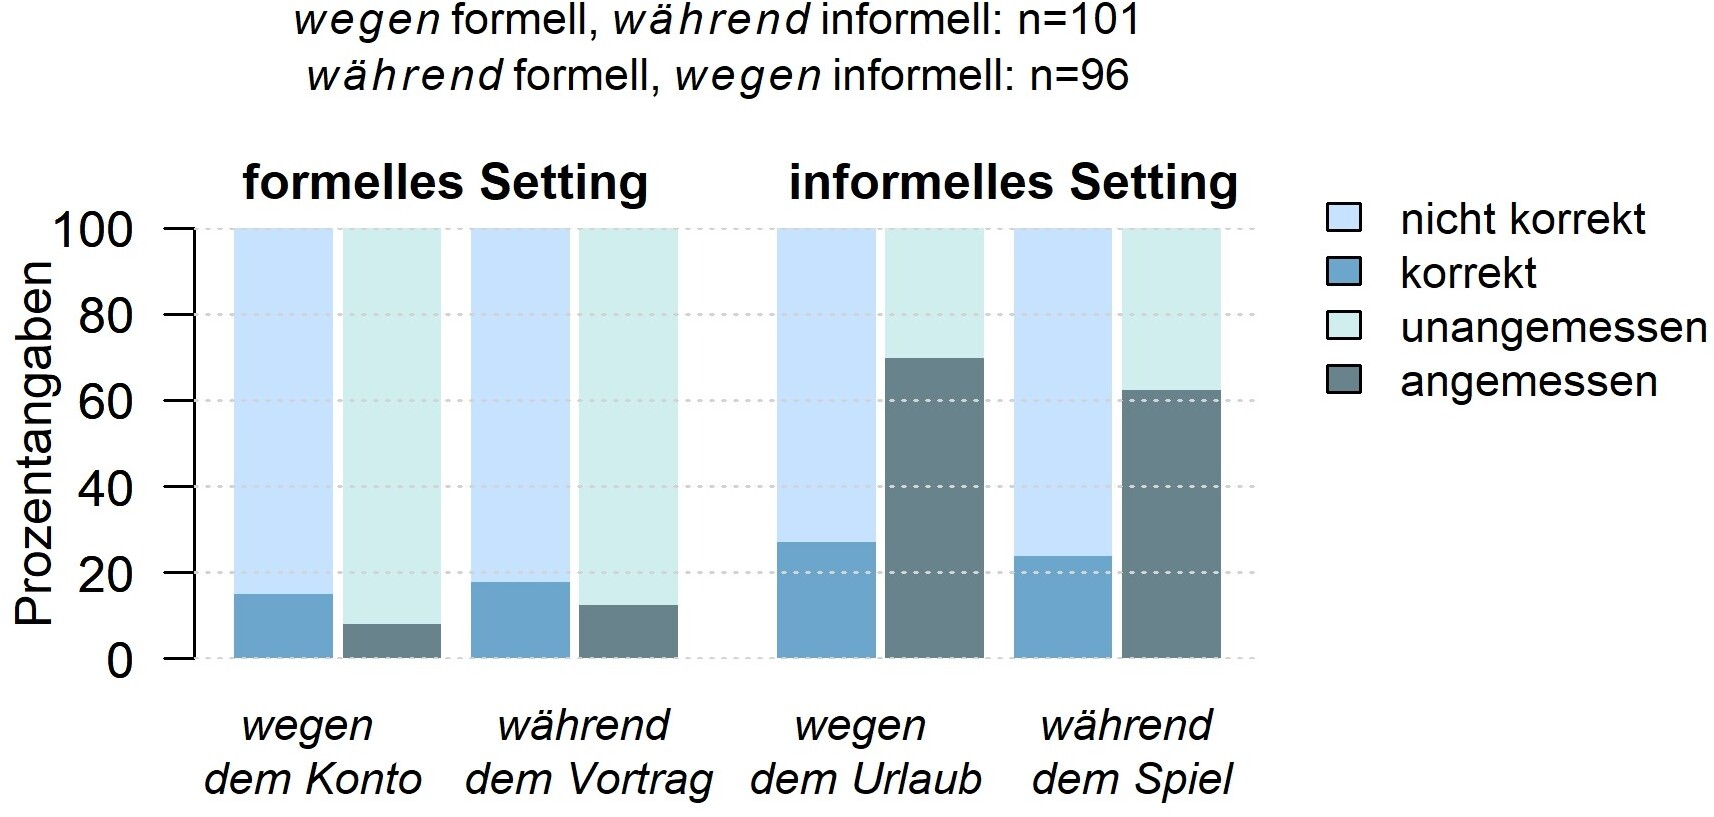
\includegraphics[scale=1]{AkzDativrektion.jpg}
\caption{Akzeptabilität der Dativrektion}
\label{pic:AkzDativrektion}
\end{figure}

Es zeigen sich deutliche Unterschiede zwischen dem formellen und dem informellen Setting. 
Interessanterweise wird dabei nicht nur die Angemessenheit situationsabhängig bewertet, sondern auch die Korrektheit. 
So wird \object{wegen dem Konto} in einem Brief an ein Amt (formelles Setting) nur von 14,9~\% der Befragten dieser Gruppe als korrekt angesehen, in einem Gespräch mit einem Freund (informelles Setting) aber empfinden 27,1~\% \object{wegen dem Urlaub} als richtig. 
Bei \waehrend{} ist der Unterschied geringer: 17,7~\% bewerten \object{während dem Vortrag} im formellen Setting als korrekt und für 23,8~\% ist \object{während dem Spiel} in einem informellen Setting korrekt. 

Große Unterschiede zwischen den beiden Settings ergeben sich in Bezug auf die Angemessenheit. 
Während nur 7,9~\% \wegen{} mit Dativrektion mit Blick auf einen formellen Brief angemessen finden, wird die Form in einem informellen Gespräch von 69,8~\% als angemessen beurteilt. 
Ganz ähnlich fallen die Angemessenheitsurteile bei \waehrend{} aus: Im formellen Brief ist die Dativrektion nur für 12,5~\% angemessen, im informellen Gespräch jedoch für 62,4~\%. 

%Der Unterschied zwischen formellem und informellem Setting wird bei der Beurteilung der Angemessenheit für beide ursprünglichen Genitivpräpositionen hochsignifikant bei mittlerer bis hoher Effektstärke. \\
Auffällig ist die starke Diskrepanz zwischen der Bewertung der Korrektheit und der Angemessenheit im informellen Kontext:
Obwohl die Dativrektion von der Mehrheit als inkorrekte Variante angesehen wird, empfindet eine ähnlich große Mehrheit sie als angemessen. 
Im formellen Kontext ist das Verhältnis zwischen Angemessenheit und Korrektheit umgekehrt: Die Dativrektion wird auch hier selten als korrekt eingestuft, als angemessen wird sie aber sogar noch etwas seltener bewertet. 

Mit dieser zweischichtigen Bewertung bringen die Befragten ihr Wissen um die Indexikalität der Varianten zum Ausdruck. 
Auf der einen Seite wissen sie, dass die Dativrektion bei \wegen{} und \waehrend{} als Fehler stigmatisiert wird, auf der anderen Seite verfügen sie über das Wissen, dass diese Rektionsvariante als informell registriert und in einem Gespräch daher durchaus zu erwarten ist. % Änderung Anfang
Zu berücksichtigen ist dabei, dass eine Diskrepanz zwischen dem Medium der beschriebenen Situation (mündlich) und dem Medium der Präsentation im Fragebogen (schriftlich) vorliegt. 
Es ist denkbar, dass die Dativvarianten bei einer tatsächlich mündlichen Präsentation noch höhere Akzeptabilitätswerte erhalten hätten. % Änderung Ende

\autoref{pic:AkzGenitivrektion} zeigt, inwiefern die Genitivrektion bei den ursprünglichen Dativpräpositionen \dank{} und \gegenueber{} akzeptiert wird (s. zusätzlich \autoref{table:AnhAkzDank} und \autoref{table:AnhAkzGegenueber} im Anhang). 
Vergleicht man die Ergebnisse bei \dank{} zwischen dem formellen und dem informellen Setting, lässt sich Folgendes feststellen: 
Die Genitivrektion bei \dank{} wird sowohl in einem Brief an ein Amt als auch in einer Unterhaltung mit einem Freund überwiegend als korrekt und angemessen eingestuft. 
Jeweils knapp über 90~\% der Befragten empfinden die Variante als korrekt. 
Die Angabe, die Genitivrektion sei unangemessen, wird im informellen Setting nur wenig häufiger getroffen als im formellen.
Damit lässt sich bereits festhalten, dass \dank{} von beinahe allen Befragten als Genitivpräposition angesehen und akzeptiert wird. 
Die Genitivrektion bei \dank{} ist -- anders als die Dativrektion bei \wegen{} und \waehrend{} -- nicht als falsch stigmatisiert und wird daher in beiden Settings gleichermaßen als angemessen empfunden. % Änderung Anfang
Hierbei könnte auch eine Rolle spielen, dass die Präposition \dank{} selbst als formell registriert ist und das Beispiel des informellen Settings daher eventuell weniger informell wahrgenommen wird.% Änderung Ende 
\begin{figure}
\centering
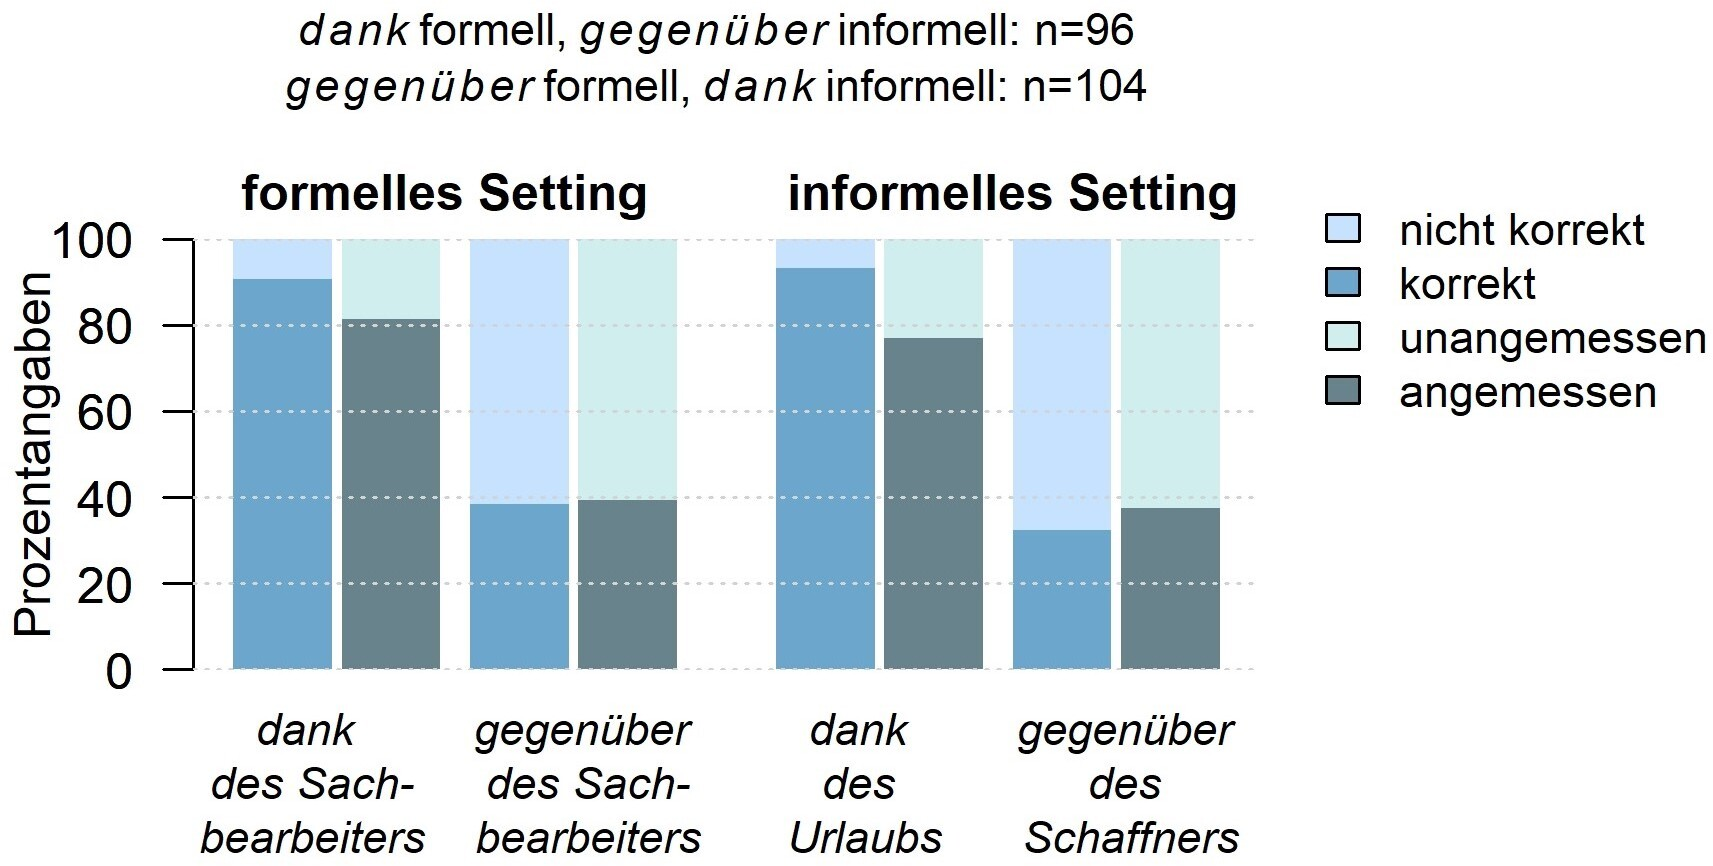
\includegraphics[scale=1]{AkzGenitivrektion.jpg}
\caption{Akzeptabilität der Genitivrektion}
\label{pic:AkzGenitivrektion}
\end{figure}

Obwohl sie laut bisherigen Untersuchungen kaum vorkommt (\autoref{sec:Differenzierung}), wird auch die Genitivrektion bei \gegenueber{} von erstaunlich vielen Befragten als korrekt empfunden:  38,5~\% bewerten  das Beispiel \object{gegenüber des Sachbearbeiters} in einem Brief an ein Amt als korrekt und immerhin 32,3~\% sehen die Genitivrektion bei \object{gegenüber des Schaffners} in einem Gespräch mit einem Freund als korrekt an.

Zwischen den Angaben zur Korrektheit und denen zur Angemessenheit ergeben sich für die Genitivrektion bei \dank{} und \gegenueber{} nur geringe Abweichungen: 
Von den meisten Befragten wird die als korrekt erachtete Form auch als angemessen empfunden bzw. umgekehrt. 

Welche Wirkung das Prestige des Genitivs entfalten kann, zeigt sich auch in den Ergebnissen des Akzeptabilitätstests zur Primärpräposition \object{seit}, die in \autoref{pic:AkzSeitKorrUAng} dargestellt sind (s. außerdem \autoref{table:AnhAkzseit} im Anhang). 
Im formellen Setting beurteilt jeweils beinahe ein Drittel der Befragten \object{seit} mit dem Genitiv als korrekt und angemessen. 
Im informellen Setting wird die Variante immerhin von knapp über 20~\% als korrekt und angemessen eingeschätzt. 
\begin{figure}
\centering
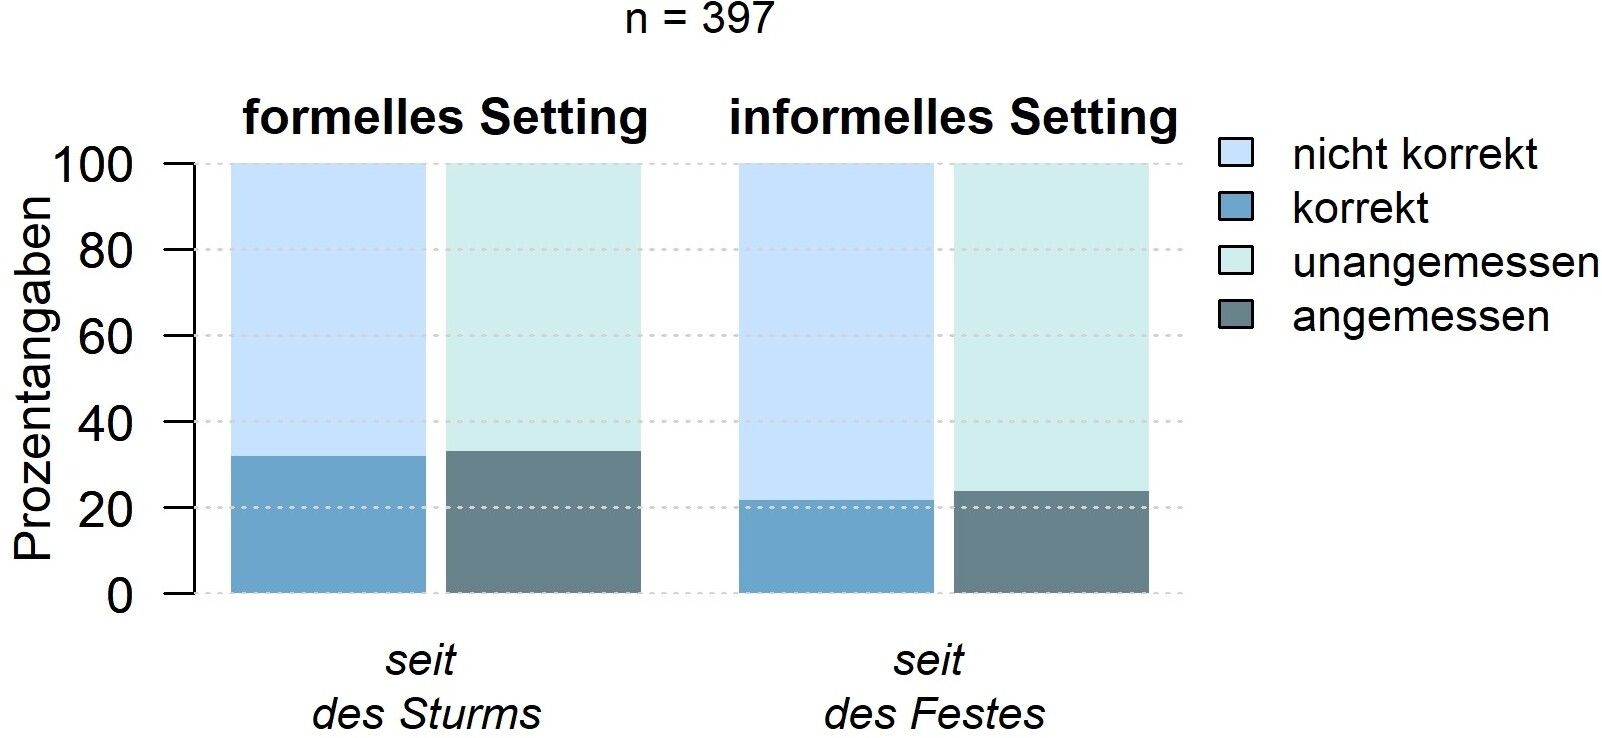
\includegraphics[scale=1]{AkzSeitKorrUAng.jpg}
\caption{Akzeptabilität der Genitivrektion bei der Primärpräposition \object{seit}}
\label{pic:AkzSeitKorrUAng}
\end{figure}

Sowohl die Ergebnisse zu \gegenueber{} als auch die Ergebnisse aus dem in \autoref{sec:Differenzierung} besprochenen Produktionsexperiment von \citet{Becker2011} zeigen, dass Sekundärpräpositionen, die laut kodifizierter Norm ausschließlich mit dem Dativ stehen können, von Befragten häufig mit dem Genitiv akzeptiert werden. 
In \citeauthor{Becker2011}s Experiment verwendeten sogar ca. 65~\% die Genitivrektion bei Präpositionen wie \object{gemäß} oder \object{entsprechend} \citep[s.][210]{Becker2011}. 
Die Ergebnisse zu \object{seit} deuten darauf hin, dass auch Primärpräpositionen, für die die Genitivrektion laut kodifizierter Norm ausgeschlossen ist (\autoref{sec:Primaer}), zu einem gewissen Grad mit dem Genitiv akzeptiert werden. 
Eventuell wird dies dadurch begünstigt, dass die Beispiele (\object{seit des Sturms} und \object{seit des Festes}) als Teile kausaler Sätze interpretiert werden könnten, wodurch \object{seit} semantisch in die Nähe von Genitivpräpositionen wie \wegen{} rückt.\footnote{Für den Hinweis auf diese Erklärungsmöglichkeit danke ich Melitta Gillmann.}
Die Konzepte \glq temporale Abfolge\grq{} und \glq Kausalität\grq{} sind metonymisch miteinander verknüpft: Das Wissen um die zeitliche Abfolge implikatiert eine Ursache-Folge-Beziehung \citep[s.][]{Traugott.1991}.
Die Entwicklung von temporalen zu kausalen Markern ist daher ein häufiger Grammatikalisierungspfad, wie bspw. die Grammatikalisierung von Subjunktionen wie \object{weil} oder \object{nachdem} zeigt \citep[s.][]{Gillmann.2018}. 

%\subsection{Angaben zur eigenen Verwendung von Genitiv- und Dativrektion}
%\label{sec:eigeneVerw}
Neben der Beurteilung von Korrektheit und Angemessenheit wurden im Akzeptabilitätstest auch Angaben dazu erhoben, ob die Befragten die Varianten in der beschriebenen Situation selbst verwenden würden. 
Wie in \autoref{sec:Spracheinstellungsforschung} besprochen, lassen Aussagen zur eigenen Verwendung nicht ohne Weiteres Rückschlüsse darauf zu, inwiefern Befragte eine Variante tatsächlich verwenden. 
Aus diesem Grund enthält der Fragebogen zusätzlich ein Produktionsexperiment.  

\autoref{pic:eigeneVerw} zeigt die Angaben zur eigenen Verwendung für alle im Akzeptabilitätstest präsentierten Varianten, d.\,h. für \dank{} und \gegenueber{} mit der Genitivrektion sowie für \wegen{} und \waehrend{} mit der Dativrektion, jeweils im formellen und im informellen Setting. 
Die Genitivrektion bei \dank{} würden laut eigenen Angaben 70,8~\% (formelles Setting) bzw. 73,1~\% (informelles Setting) selbst verwenden. 
Das sind jeweils etwas weniger Befragte als diejenigen, die angeben, dass diese Variante angemessen sei und deutlich weniger (jeweils ca. 20~\%) als diejenigen, die die Variante als korrekt erachten (vgl. \autoref{pic:AkzGenitivrektion}). 
\object{Gegenüber} mit Genitivrektion erhält wie bereits bei der Beurteilung von Korrektheit und Angemessenheit überraschend hohe Werte: 
31,7~\% geben an, dass sie die Form in einem formellen Brief selbst verwenden würden, und 21,8~\% schätzen, dass sie diese Variante in einer informellen Unterhaltung gebrauchen würden. 
Auch hier liegen die Werte jeweils etwas unter denen zu Korrektheit und Angemessenheit. 
Dass die Anzahl Befragter, die angeben, die Formen selbst zu verwenden, geringer ist als die Anzahl Befragter, die die Formen korrekt oder angemessen finden, deutet evtl. auf Unsicherheiten bei der Beurteilung der Beispiele hin. 
%Inwiefern die Befragten ihren Gebrauch einer Variante evtl. über- oder unterschätzen, wird in \autoref{sec:ProdNachAkz} anhand des Vergleichs mit den Ergebnissen aus dem Produktionsexperiment untersucht. 
\begin{figure}
\centering
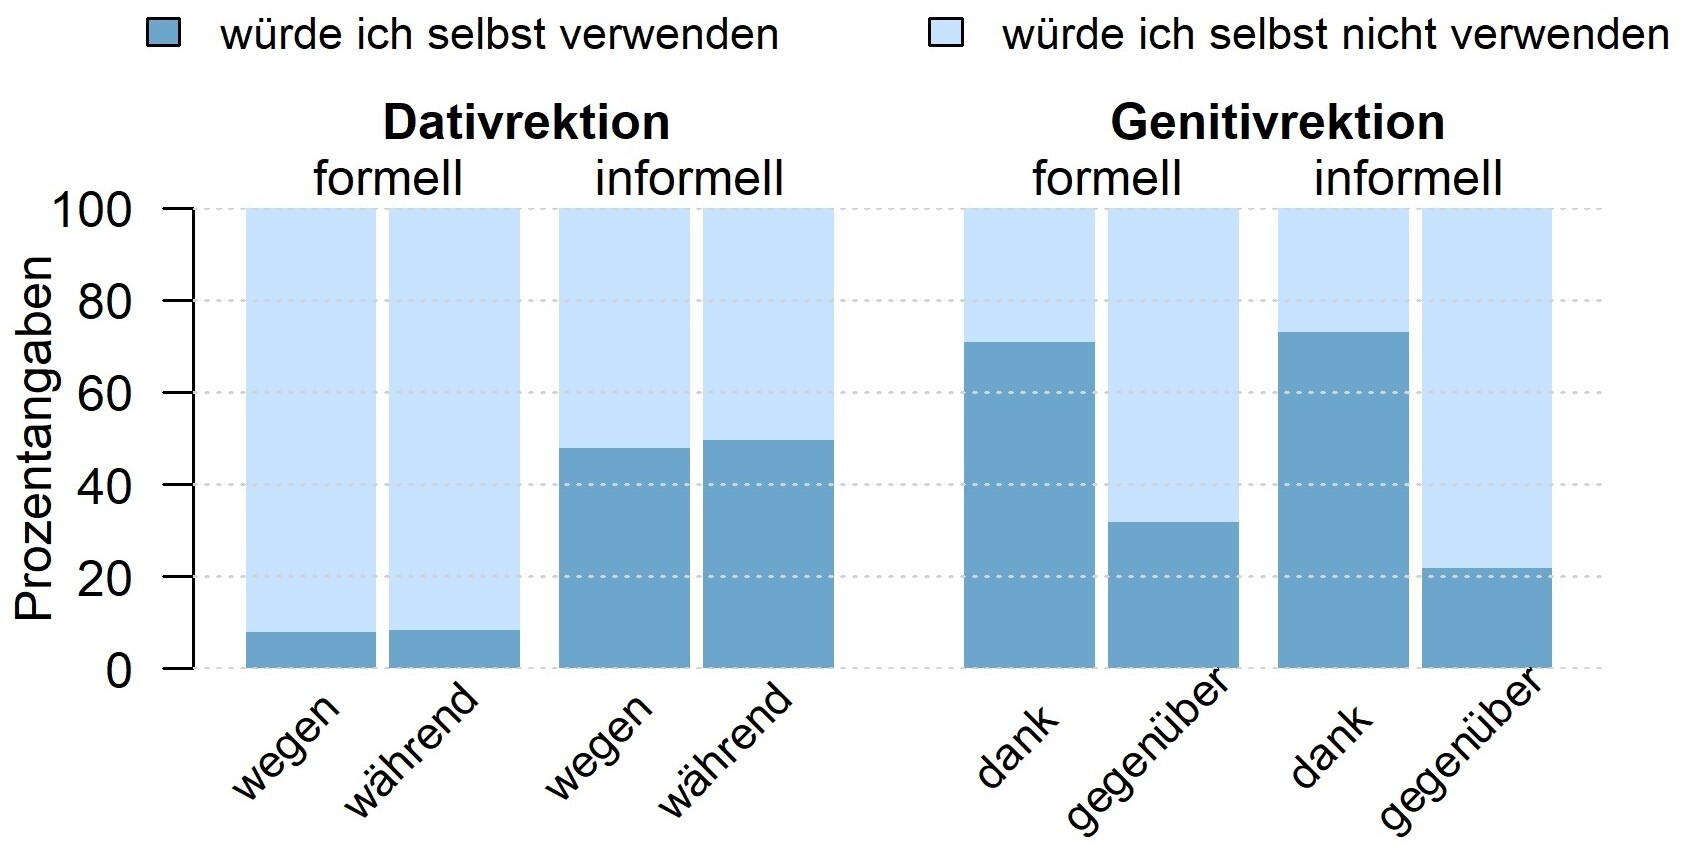
\includegraphics[width=\textwidth]{eigeneVerw.jpg}
\caption{Angaben zur eigenen Verwendung}
\label{pic:eigeneVerw}
\end{figure}

Anders als bei der Genitivrektion zeigen sich bei den Angaben zur eigenen Verwendung der Dativrektion große Unterschiede zwischen dem formellen und dem informellen Setting, wie dies bereits bei der Beurteilung von Korrektheit und Angemessenheit der Fall war. 
Nur 7,9~\% geben an, in einem Brief an ein Amt \wegen{} mit dem Dativ zu verwenden, 8,3~\% sind es bei \waehrend{} mit dem Dativ. 
In einem Gespräch unter Freunden hingegen können sich bei \wegen{} 47,9~\% vorstellen, die Dativrektion zu gebrauchen, bei \waehrend{} 49,5~\%. 
Umgekehrt heißt dies aber auch, dass die Hälfte der Befragten laut eigenen Angaben auch in einer informellen mündlichen Situation den Genitiv mit \wegen{} und \waehrend{} gebrauchen würde, im Falle von \dank{} sogar beinahe drei Viertel. 
Insgesamt schätzen die Befragten also bei Genitivvarianten eher, dass sie diese selbst verwenden würden.
%EVTL NOCH ZUSAMMENFASSENDE ABBILDUNG, IN DER AKZEPTABILITÄT UND VERWENDUNG ZU SEHEN SIND

Die Auswertung der Frage \glqq würden Sie die Variante selbst verwenden?\grqq{} bei \object{seit} mit der Genitivrektion lässt sich \autoref{pic:eigeneVerwSeit} entnehmen. 
Auch bei der Primärpräposition \object{seit} gibt beinahe ein Drittel der Befragten (28~\%) an, die Genitivrektion in einem formellen Brief potenziell selbst zu verwenden. 
Hingegen geben nur ca. 13~\% an, dass sie \object{seit} mit dem Genitiv in einem informellen Gespräch selbst verwenden würden, obwohl über 20~\% die Variante hier als korrekt und angemessen bewerten (s. \autoref{pic:AkzSeitKorrUAng}). 
Auch wenn die Zustimmungswerte für die eigene Verwendung bei \object{seit} geringer sind als bei den anderen Genitivvarianten, muss festgehalten werden, dass sich insbesondere in einem formellen Kontext recht viele Befragte vorstellen können, den Genitiv bei \object{seit} zu verwenden. 
\begin{figure}
\centering
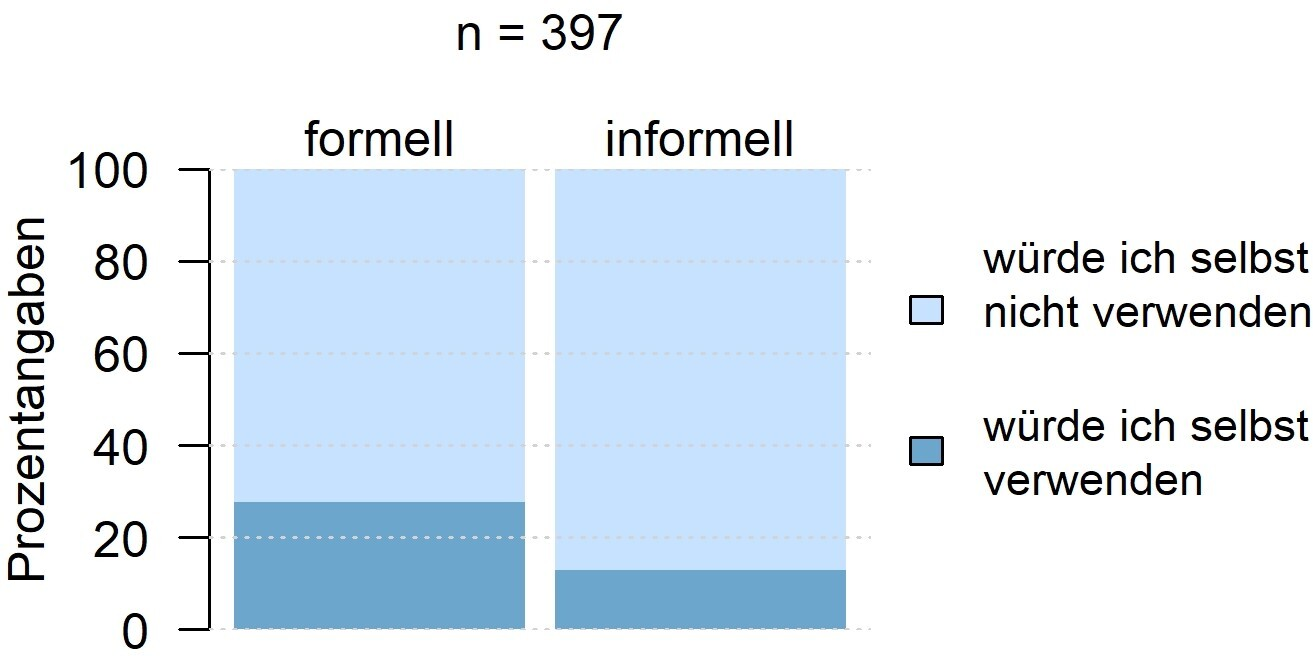
\includegraphics[scale=1]{eigeneVerwSeit.jpg}
\caption{Angaben zur eigenen Verwendung der Primärpräposition \object{seit} mit dem Genitiv}
\label{pic:eigeneVerwSeit}
\end{figure}

Die Auswertung der Angaben zu Korrektheit, Angemessenheit und eigener Verwendung im Vergleich zwischen dem formellen und dem informellen Setting lässt sich folgendermaßen zusammenfassen:
Tendenziell erzielen die Genitivvarianten (\dank{}, \gegenueber{} und \object{seit} plus Genitiv) höhere Akzeptabilitätswerte als die Dativvarianten (\wegen{} und \waehrend{} plus Dativ). 
Die Genitivrektion wird selbst mit der Primärpräposition \object{seit} in beiden Settings von mehr als 20~\% der Befragten als korrekt und angemessen bewertet, während die Dativrektion mit \wegen{} und \waehrend{} im formellen Setting von jeweils unter 20~\% als korrekt oder angemessen eingestuft wird. 
Die Dativrektion bei den ursprünglichen Genitivpräpositionen \wegen{} und \waehrend{} wird kontextabhängig bewertet.
Sie gilt im informellen Setting etwas häufiger als korrekt und deutlich häufiger als angemessen als im formellen Setting. 
Bei der Bewertung der Genitivrektion bei \dank{}, \gegenueber{} und \object{seit} fallen die Unterschiede zwischen den Settings geringer aus.  
Bei allen fünf Präpositionen scheint für die Befragten die Angemessenheit im formellen Setting weitgehend mit der Korrektheit zusammenzufallen, während die Bewertung beider Dimensionen im informellen Setting auseinandergehen kann. 
Die folgenden Abschnitte beschäftigen sich damit, inwiefern sich die Angaben zu Korrektheit, Angemessenheit und der eigenen Verwendung der Varianten in verschiedenen Befragtengruppen unterscheiden. 
\subsection{Akzeptabilität und Alter}
\label{sec:ErgAkzNachAlter}
%Akzeptabilität und Alter
% Änderung!
Da es sich bei Kasusschwankungen von Sekundärpräpositionen um ein Sprachwandelpänomen handelt, ist es entsprechend dem \textit{apparent-time}-Ansatz Labovs eine naheliegende Vermutung, dass sich ältere und jüngere SprachbenutzerInnen in ihrer Bewertung der Varianten unterscheiden (\citealp[s.][40]{Preston.1991}). 
\citet[313]{Bailey.2004} fasst diesen Ansatz wie folgt zusammen:
\begin{quote}Labov hypothesized that when social and stylistic factors were held constant, linguistic differences among different generations of a population (apparent-time differences) would mirror actual diachronic developments in the language (real-time linguistic changes).\end{quote}
% Ende Änderung
Im Folgenden wird daher untersucht, wie die Angaben zu Korrektheit, Angemessenheit und eigener Verwendung der im Akzeptabilitätstest abgefragten Rektionsvarianten mit dem Alter der Befragten zusammenhängen. 
Dafür wird die jüngste Gruppe der Befragten (18 bis 25 Jahre) mit der ältesten Gruppe der Befragten (61 bis 85 Jahre) verglichen. 
Für alle fünf Präpositionen (\wegen{}, \waehrend{}, \dank{}, \gegenueber{} und \object{seit}) werden jeweils die Akzeptabilitätswerte im formellen sowie im informellen Setting betrachtet.

Beim Vergleich der jüngsten mit den ältesten Befragten muss berücksichtigt werden, dass die beiden Altersgruppen sich auch in anderen soziodemografischen Merkmalen unterscheiden (\autoref{sec:Befragte}):
Unter den über 60-jährigen Befragten finden sich mehr Personen ohne Abitur und deutlich mehr Norddeutsche als unter den 18- bis 25-jährigen Befragten.\footnote{Der Anteil an Befragten ohne Hochschulabschluss ist zwar in beiden Altersgruppen etwa gleich, jedoch befinden sich viele der unter 26-jährigen Befragten gerade im Studium und haben dieses noch nicht abgeschlossen (\autoref{sec:Bildung}).} 

Da die BefragungsteilnehmerInnen für den Akzeptabilitätstest auf vier Gruppen verteilt wurden (s. \autoref{table:AkzBsp} und \autoref{sec:Akz}), finden sich pro Gruppe jeweils nur recht wenige Befragte für jede Altersgruppe. 
Aus diesem Grund werden die beiden Gruppen, die im Akzeptabilitätstest die Präpositionen \wegen{} und \waehrend{} bewertet haben, hier zusammen betrachtet. 
%Zur Erinnerung: Die Gruppen unterscheiden sich darin, welche der beiden Präpositionen im informellen Kontext (Gespräch mit einem Freund) und welche im formellen Kontext (Brief an ein Amt) bewertet wurde. 
\object{Wegen} und \waehrend{} gemeinsam zu betrachten, bietet sich an, da beide Präpositionen ein ähnliches sprachhistorisches Profil haben und heute zu einem ähnlichen Maß Rektionsschwankungen zeigen (\autoref{cha:SekPraeps}). 
In beiden Gruppen zusammen sind 51 Befragte zwischen 18 und 25 Jahren und 29 Befragte zwischen 61 und 85 Jahren, wie aus \autoref{table:ErgAkzDativNachAlter} hervorgeht. 
Von den 51 Jüngeren haben dabei 26 \wegen{} plus Dativ im formellen und \waehrend{} plus Dativ im informellen Setting bewertet, 25 beurteilten hingegen \wegen{} plus Dativ im informellen Setting und \waehrend{} plus Dativ im formellen. 
Von den 29 älteren Befragten bewerteten 14 \wegen{} plus Dativ im formellen und \waehrend{} plus Dativ im informellen Setting sowie 15 umgekehrt \wegen{} plus Dativ im informellen Setting und \waehrend{} plus Dativ im formellen.
\autoref{table:ErgAkzDativNachAlter} zeigt die addierten Zahlen beider Gruppen, getrennt nach Altersgruppen. 
Angegeben sind jeweils die absoluten Zahlen sowie die Prozentwerte.\footnote{Aufgrund von Rundungsungenauigkeiten kann es dazu kommen, dass die addierten Prozentwerte nicht genau 100 ergeben.}
Letztere dienen nur der besseren Lesbarkeit beim Vergleich der beiden Gruppen und sind aufgrund der geringen Stichprobengröße mit Vorsicht zu betrachten. 
% Please add the following required packages to your document preamble:
% \usepackage{multirow}
% \usepackage[table,xcdraw]{xcolor}
% If you use beamer only pass "xcolor=table" option, i.e. \documentclass[xcolor=table]{beamer}
\begin{table}
\centering
\begin{tabular}{llrrrr}
\multicolumn{6}{l}{\wegen{} oder \waehrend{} + Dativ nach Alter}                                                                                                                                                                                                                          \\ \hline
                                                                                &                                      & \multicolumn{2}{c}{\begin{tabular}[c]{@{}c@{}}18--25 Jahre\\ (n=51)\end{tabular}} & \multicolumn{2}{c}{\begin{tabular}[c]{@{}c@{}}61--85 Jahre\\ (n=29)\end{tabular}} \\ \hline
                                                                                & \cellcolor[HTML]{9B9B9B}korrekt      & \cellcolor[HTML]{9B9B9B}10          & \cellcolor[HTML]{9B9B9B}{\footnotesize (19,61 \%)}         & \cellcolor[HTML]{9B9B9B}3           & \cellcolor[HTML]{9B9B9B}{\footnotesize (10,34 \%)}         \\ %\cline{2-6} 
                                                                                & \cellcolor[HTML]{9B9B9B}inkorrekt    & \cellcolor[HTML]{9B9B9B}41          & \cellcolor[HTML]{9B9B9B}{\footnotesize (80,39 \%)}         & \cellcolor[HTML]{9B9B9B}26          & \cellcolor[HTML]{9B9B9B}{\footnotesize (89,66 \%)}         \\ %\cline{2-6} 
                                                                                & \cellcolor[HTML]{EFEFEF}angemessen   & \cellcolor[HTML]{EFEFEF}6           & \cellcolor[HTML]{EFEFEF}{\footnotesize (11,76 \%)}         & \cellcolor[HTML]{EFEFEF}1           & \cellcolor[HTML]{EFEFEF}{\footnotesize (3,45 \%)}          \\ %\cline{2-6} 
                                                                                & \cellcolor[HTML]{EFEFEF}unangemessen & \cellcolor[HTML]{EFEFEF}45          & \cellcolor[HTML]{EFEFEF}{\footnotesize (88,24 \%)}         & \cellcolor[HTML]{EFEFEF}28          & \cellcolor[HTML]{EFEFEF}{\footnotesize (96,55 \%)}         \\ %\cline{2-6} 
                                                                                & eigene Verwendung ja                 & 8                                   & {\footnotesize (15,69 \%)}                                 & 0                                   & {\footnotesize (0 \%)}                                     \\ %\cline{2-6} 
\multirow{-6}{*}{\begin{tabular}[c]{@{}l@{}}formelles\\ Setting\end{tabular}}   & eigene Verwendung nein               & 43                                  & {\footnotesize (84,31 \%})                                 & 29                                  & {\footnotesize (100 \%)}                                   \\ \hline
                                                                                &                                      & \multicolumn{2}{c}{\begin{tabular}[c]{@{}c@{}}18--25 Jahre\\ (n=51)\end{tabular}} & \multicolumn{2}{c}{\begin{tabular}[c]{@{}c@{}}61--85 Jahre\\ (n=29)\end{tabular}} \\ \hline
                                                                                & \cellcolor[HTML]{9B9B9B}korrekt      & \cellcolor[HTML]{9B9B9B}15          & \cellcolor[HTML]{9B9B9B}{\footnotesize (29,41 \%)}         & \cellcolor[HTML]{9B9B9B}4           & \cellcolor[HTML]{9B9B9B}{\footnotesize (13,79 \%)}         \\ %\cline{2-6} 
                                                                                & \cellcolor[HTML]{9B9B9B}inkorrekt    & \cellcolor[HTML]{9B9B9B}36          & \cellcolor[HTML]{9B9B9B}{\footnotesize (70,59 \%)}         & \cellcolor[HTML]{9B9B9B}25          & \cellcolor[HTML]{9B9B9B}{\footnotesize (86,21 \%)}         \\ %\cline{2-6} 
                                                                                & \cellcolor[HTML]{EFEFEF}angemessen   & \cellcolor[HTML]{EFEFEF}42          & \cellcolor[HTML]{EFEFEF}{\footnotesize (82,35 \%)}         & \cellcolor[HTML]{EFEFEF}10          & \cellcolor[HTML]{EFEFEF}{\footnotesize (34,48 \%)}         \\ %\cline{2-6} 
                                                                                & \cellcolor[HTML]{EFEFEF}unangemessen & \cellcolor[HTML]{EFEFEF}9           & \cellcolor[HTML]{EFEFEF}{\footnotesize (17,65 \%)}         & \cellcolor[HTML]{EFEFEF}19          & \cellcolor[HTML]{EFEFEF}{\footnotesize (65,52 \%)}         \\ %\cline{2-6} 
                                                                                & eigene Verwendung ja                 & 31                                  & {\footnotesize (60,78 \%)}                                 & 7                                   & {\footnotesize (24,14 \%)}                                 \\ %\cline{2-6} 
\multirow{-6}{*}{\begin{tabular}[c]{@{}l@{}}informelles\\ Setting\end{tabular}} & eigene Verwendung nein               & 20                                  & {\footnotesize (39,22 \%)}                                 & 22                                  & {\footnotesize (75,86 \%)}                                 \\ \hline
\end{tabular}
\caption{Akzeptabilität der Dativrektion bei \wegen{} und \waehrend{} nach Alter}
\label{table:ErgAkzDativNachAlter}
\end{table}

Der größte Unterschied zwischen den jüngeren und den älteren Befragten ist die Bewertung der Angemessenheit im informellen Setting: 
Die deutliche Mehrheit der Befragten zwischen 18 und 25 empfindet die Dativrektion bei \wegen{} oder \waehrend{} als angemessen (42 von 51). 
Nur ein Drittel der älteren Befragten teilt diese Einschätzung (zehn von 29). 
Auch die Angaben zur eigenen Verwendung unterscheiden sich deutlich. 
Während eine Mehrheit der jüngeren Befragten den Dativ in einem informellen Kontext verwenden würde (31 von 51), gibt nur eine Minderheit der älteren Befragten an, dies zu tun (sieben von 29). 
In beiden Altersgruppen zeigen dich Unterschiede zwischen der Akzeptabilität im formellen und im informellen Setting, jedoch sind diese in der Gruppe der 18- bis 25-Jährigen größer.
Die jüngere Gruppe scheint also etwas kontextsensitiver zu sein als die ältere Gruppe. 
Auch die Diskrepanz zwischen der Bewertung der Korrektheit und der Bewertung der Angemessenheit ist in der Gruppe der jüngeren Befragten größer als unter den über 60-Jährigen. 

Um mögliche Altersunterschiede bei der Akzeptabilität der Genitivrektion zu identifizieren, wird zunächst nur die Präposition \dank{} betrachtet (s. \autoref{table:ErgAkzDankNachAlter}). 
Die Ergebnisse zu \dank{} mit denen zu \gegenueber{} zusammenzurechnen, wird vermieden, da diese beiden Präpositionen zu verschieden sind: 
Während der Genitiv bei \dank{} bereits etabliert ist, kommt er bei \gegenueber{} noch kaum vor (\autoref{cha:SekPraeps}). 
Die Stichproben sind hier daher deutlich kleiner als bei der Betrachtung der Akzeptabilität der Dativrektion. 
Dies liegt an der vom Zufallsmechanismus des Fragebogens vorgenommenen Gruppeneinteilung. 
In die Gruppe, die \dank{} plus Genitiv im formellen Setting bewertete, wurden vom Zufallsgenerator 29 Befragte zwischen 18 und 25 und neun Befragte über 60 eingeteilt. 
Im informellen Setting bewerteten 24 jüngere und neun ältere Befragte \dank{} plus Genitiv. 
Die Zahlen in \autoref{table:ErgAkzDankNachAlter} lassen kaum nennenswerte Unterschiede zwischen jüngeren und älteren Befragten erkennen. 
Zwar lehnt unter den Befragten über 60 ein größerer Anteil \dank{} plus Genitiv im informellen Kontext als unangemessen ab, jedoch lässt sich dies aufgrund der geringen Zahlen nicht interpretieren. 
% Please add the following required packages to your document preamble:
% \usepackage{multirow}
% \usepackage[table,xcdraw]{xcolor}
% If you use beamer only pass "xcolor=table" option, i.e. \documentclass[xcolor=table]{beamer}
\begin{table}
\centering
\begin{tabular}{llrrrr}
\multicolumn{6}{l}{\dank{} + Genitiv nach Alter}                                                                                                                                                                                                                                      \\ \hline
                                                                                &                                      & \multicolumn{2}{c}{\begin{tabular}[c]{@{}c@{}}18--25 Jahre\\ (n=29)\end{tabular}} & \multicolumn{2}{c}{\begin{tabular}[c]{@{}c@{}}61--85 Jahre\\ (n=9)\end{tabular}} \\ \hline
                                                                                & \cellcolor[HTML]{9B9B9B}korrekt      & \cellcolor[HTML]{9B9B9B}28          & \cellcolor[HTML]{9B9B9B}{\footnotesize (96,55 \%)}         & \cellcolor[HTML]{9B9B9B}8          & \cellcolor[HTML]{9B9B9B}{\footnotesize (88,89 \%)}         \\ %\cline{2-6} 
                                                                                & \cellcolor[HTML]{9B9B9B}inkorrekt    & \cellcolor[HTML]{9B9B9B}1           & \cellcolor[HTML]{9B9B9B}{\footnotesize (3,45 \%)}          & \cellcolor[HTML]{9B9B9B}1          & \cellcolor[HTML]{9B9B9B}{\footnotesize (11,11 \%)}         \\ %\cline{2-6} 
                                                                                & \cellcolor[HTML]{EFEFEF}angemessen   & \cellcolor[HTML]{EFEFEF}25          & \cellcolor[HTML]{EFEFEF}{\footnotesize (86,21 \%)}         & \cellcolor[HTML]{EFEFEF}6          & \cellcolor[HTML]{EFEFEF}{\footnotesize (66,67 \%)}         \\ %\cline{2-6} 
                                                                                & \cellcolor[HTML]{EFEFEF}unangemessen & \cellcolor[HTML]{EFEFEF}4           & \cellcolor[HTML]{EFEFEF}{\footnotesize (13,79 \%)}         & \cellcolor[HTML]{EFEFEF}3          & \cellcolor[HTML]{EFEFEF}{\footnotesize (33,33 \%)}         \\ %\cline{2-6} 
                                                                                & eigene Verwendung ja                 & 24                                  & {\footnotesize (82,76 \%)}                                 & 6                                  & {\footnotesize (66,67 \%)}                                 \\ %\cline{2-6} 
\multirow{-6}{*}{\begin{tabular}[c]{@{}l@{}}formelles\\ Setting\end{tabular}}   & eigene Verwendung nein               & 5                                   & {\footnotesize (17,24 \%)}                                 & 3                                  & {\footnotesize (33,33 \%)}                                 \\ \hline
                                                                                &                                      & \multicolumn{2}{c}{\begin{tabular}[c]{@{}c@{}}18--25 Jahre\\ (n=24)\end{tabular}} & \multicolumn{2}{c}{\begin{tabular}[c]{@{}c@{}}61--85 Jahre\\ (n=9)\end{tabular}} \\ \hline
                                                                                & \cellcolor[HTML]{9B9B9B}korrekt      & \cellcolor[HTML]{9B9B9B}21          & \cellcolor[HTML]{9B9B9B}{\footnotesize (87,5 \%)}          & \cellcolor[HTML]{9B9B9B}7          & \cellcolor[HTML]{9B9B9B}{\footnotesize (77,78 \%)}         \\ %\cline{2-6} 
                                                                                & \cellcolor[HTML]{9B9B9B}inkorrekt    & \cellcolor[HTML]{9B9B9B}3           & \cellcolor[HTML]{9B9B9B}{\footnotesize (12,5 \%)}          & \cellcolor[HTML]{9B9B9B}2          & \cellcolor[HTML]{9B9B9B}{\footnotesize (22,22 \%)}         \\ %\cline{2-6} 
                                                                                & \cellcolor[HTML]{EFEFEF}angemessen   & \cellcolor[HTML]{EFEFEF}19          & \cellcolor[HTML]{EFEFEF}{\footnotesize (79,17 \%)}         & \cellcolor[HTML]{EFEFEF}5          & \cellcolor[HTML]{EFEFEF}{\footnotesize (55,56 \%)}         \\ %\cline{2-6} 
                                                                                & \cellcolor[HTML]{EFEFEF}unangemessen & \cellcolor[HTML]{EFEFEF}5           & \cellcolor[HTML]{EFEFEF}{\footnotesize (20,83 \%)}         & \cellcolor[HTML]{EFEFEF}4          & \cellcolor[HTML]{EFEFEF}{\footnotesize (44,44 \%)}         \\ %\cline{2-6} 
                                                                                & eigene Verwendung ja                 & 18                                  & {\footnotesize (75 \%)}                                    & 6                                  & {\footnotesize (66,67 \%)}                                 \\ %\cline{2-6} 
\multirow{-6}{*}{\begin{tabular}[c]{@{}l@{}}informelles\\ Setting\end{tabular}} & eigene Verwendung nein               & 6                                   & {\footnotesize (25 \%)}                                    & 3                                  & {\footnotesize (33,33 \%)}                                 \\ \hline
\end{tabular}
\caption{Akzeptabilität der Genitivrektion bei dank nach Alter}
\label{table:ErgAkzDankNachAlter}
\end{table}

Die Genitivrektion bei \gegenueber{} wurde im formellen Setting von 24 Befragten aus der jüngsten und neun Befragten aus der ältesten Altersgruppe bewertet. 
Im informellen Setting bekamen diese Variante aufgrund des Zufallsgenerators 29 Befragte zwischen 18 und 25 und neun Befragte über 60. 
Betrachtet man die Akzeptabilität der Genitivrektion bei \gegenueber{} in den beiden Altersgruppen, lassen sich mögliche Unterschiede im formellen Setting erkennen (s. \autoref{table:ErgAkzGegenueberNachAlter}). 
Jeweils ca. die Hälfte der insgesamt 24 18- bis 25-jährigen Befragten empfindet die Variante als korrekt und angemessen und würde sie selbst verwenden. 
Acht von neun über 60-Jährigen lehnen sie hingegen als inkorrekt ab, alle neun bewerten sie als unangemessen. 
% Please add the following required packages to your document preamble:
% \usepackage{multirow}
% \usepackage[table,xcdraw]{xcolor}
% If you use beamer only pass "xcolor=table" option, i.e. \documentclass[xcolor=table]{beamer}
\begin{table}
\centering
\begin{tabular}{llrrrr}
\multicolumn{6}{l}{\gegenueber{} + Genitiv nach Alter}                                                                                                                                                                                                                                \\ \hline
                                                                                &                                      & \multicolumn{2}{c}{\begin{tabular}[c]{@{}c@{}}18--25 Jahre\\ (n=24)\end{tabular}} & \multicolumn{2}{c}{\begin{tabular}[c]{@{}c@{}}61--85 Jahre\\ (n=9)\end{tabular}} \\ \hline
                                                                                & \cellcolor[HTML]{9B9B9B}korrekt      & \cellcolor[HTML]{9B9B9B}12          & \cellcolor[HTML]{9B9B9B}{\footnotesize (50 \%)}            & \cellcolor[HTML]{9B9B9B}1          & \cellcolor[HTML]{9B9B9B}{\footnotesize (11,11 \%)}         \\ %\cline{2-6} 
                                                                                & \cellcolor[HTML]{9B9B9B}inkorrekt    & \cellcolor[HTML]{9B9B9B}12          & \cellcolor[HTML]{9B9B9B}{\footnotesize (50 \%)}            & \cellcolor[HTML]{9B9B9B}8          & \cellcolor[HTML]{9B9B9B}{\footnotesize (88,89 \%)}         \\ %\cline{2-6} 
                                                                                & \cellcolor[HTML]{EFEFEF}angemessen   & \cellcolor[HTML]{EFEFEF}11          & \cellcolor[HTML]{EFEFEF}{\footnotesize (45,83 \%)}         & \cellcolor[HTML]{EFEFEF}0          & \cellcolor[HTML]{EFEFEF}{\small (0 \%)}             \\ %\cline{2-6} 
                                                                                & \cellcolor[HTML]{EFEFEF}unangemessen & \cellcolor[HTML]{EFEFEF}13          & \cellcolor[HTML]{EFEFEF}{\footnotesize (54,17 \%)}         & \cellcolor[HTML]{EFEFEF}9          & \cellcolor[HTML]{EFEFEF}{\footnotesize (100 \%)}           \\ %\cline{2-6} 
                                                                                & eigene Verwendung ja                 & 11                                  & {\footnotesize (45,83 \%)}                                 & 0                                  & {\footnotesize (0 \%)}                                     \\ %\cline{2-6} 
\multirow{-6}{*}{\begin{tabular}[c]{@{}l@{}}formelles\\ Setting\end{tabular}}   & eigene Verwendung nein               & 13                                  & {\footnotesize (54,17 \%)}                                 & 9                                  & {\footnotesize (100 \%)}                                   \\ \hline
                                                                                &                                      & \multicolumn{2}{c}{\begin{tabular}[c]{@{}c@{}}18--25 Jahre\\ (n=29)\end{tabular}} & \multicolumn{2}{c}{\begin{tabular}[c]{@{}c@{}}61--85 Jahre\\ (n=9)\end{tabular}} \\ \hline
                                                                                & \cellcolor[HTML]{9B9B9B}korrekt      & \cellcolor[HTML]{9B9B9B}13          & \cellcolor[HTML]{9B9B9B}{\footnotesize (44,83 \%)}         & \cellcolor[HTML]{9B9B9B}4          & \cellcolor[HTML]{9B9B9B}{\footnotesize (44,44 \%)}         \\ %\cline{2-6} 
                                                                                & \cellcolor[HTML]{9B9B9B}inkorrekt    & \cellcolor[HTML]{9B9B9B}16          & \cellcolor[HTML]{9B9B9B}{\footnotesize (55,17 \%)}         & \cellcolor[HTML]{9B9B9B}5          & \cellcolor[HTML]{9B9B9B}{\footnotesize (55,56 \%)}         \\ %\cline{2-6} 
                                                                                & \cellcolor[HTML]{EFEFEF}angemessen   & \cellcolor[HTML]{EFEFEF}13          & \cellcolor[HTML]{EFEFEF}{\footnotesize (44,83 \%)}         & \cellcolor[HTML]{EFEFEF}3          & \cellcolor[HTML]{EFEFEF}{\footnotesize (33,33 \%)}         \\ %\cline{2-6} 
                                                                                & \cellcolor[HTML]{EFEFEF}unangemessen & \cellcolor[HTML]{EFEFEF}16          & \cellcolor[HTML]{EFEFEF}{\footnotesize (55,17 \%)}         & \cellcolor[HTML]{EFEFEF}6          & \cellcolor[HTML]{EFEFEF}{\footnotesize (66,67 \%)}         \\ %\cline{2-6} 
                                                                                & eigene Verwendung ja                 & 6                                   & {\footnotesize (20,69 \%)}                                 & 3                                  & {\footnotesize (33,33 \%)}                                 \\ %\cline{2-6} 
\multirow{-6}{*}{\begin{tabular}[c]{@{}l@{}}informelles\\ Setting\end{tabular}} & eigene Verwendung nein               & 23                                  & {\footnotesize (79,31 \%)}                                 & 6                                  & {\footnotesize (66,67 \%)}                                 \\ \hline
\end{tabular}
\caption{Akzeptabilität der Genitivrektion bei \gegenueber{} nach Alter}
\label{table:ErgAkzGegenueberNachAlter}
\end{table}
%\begin{figure}
%\centering
%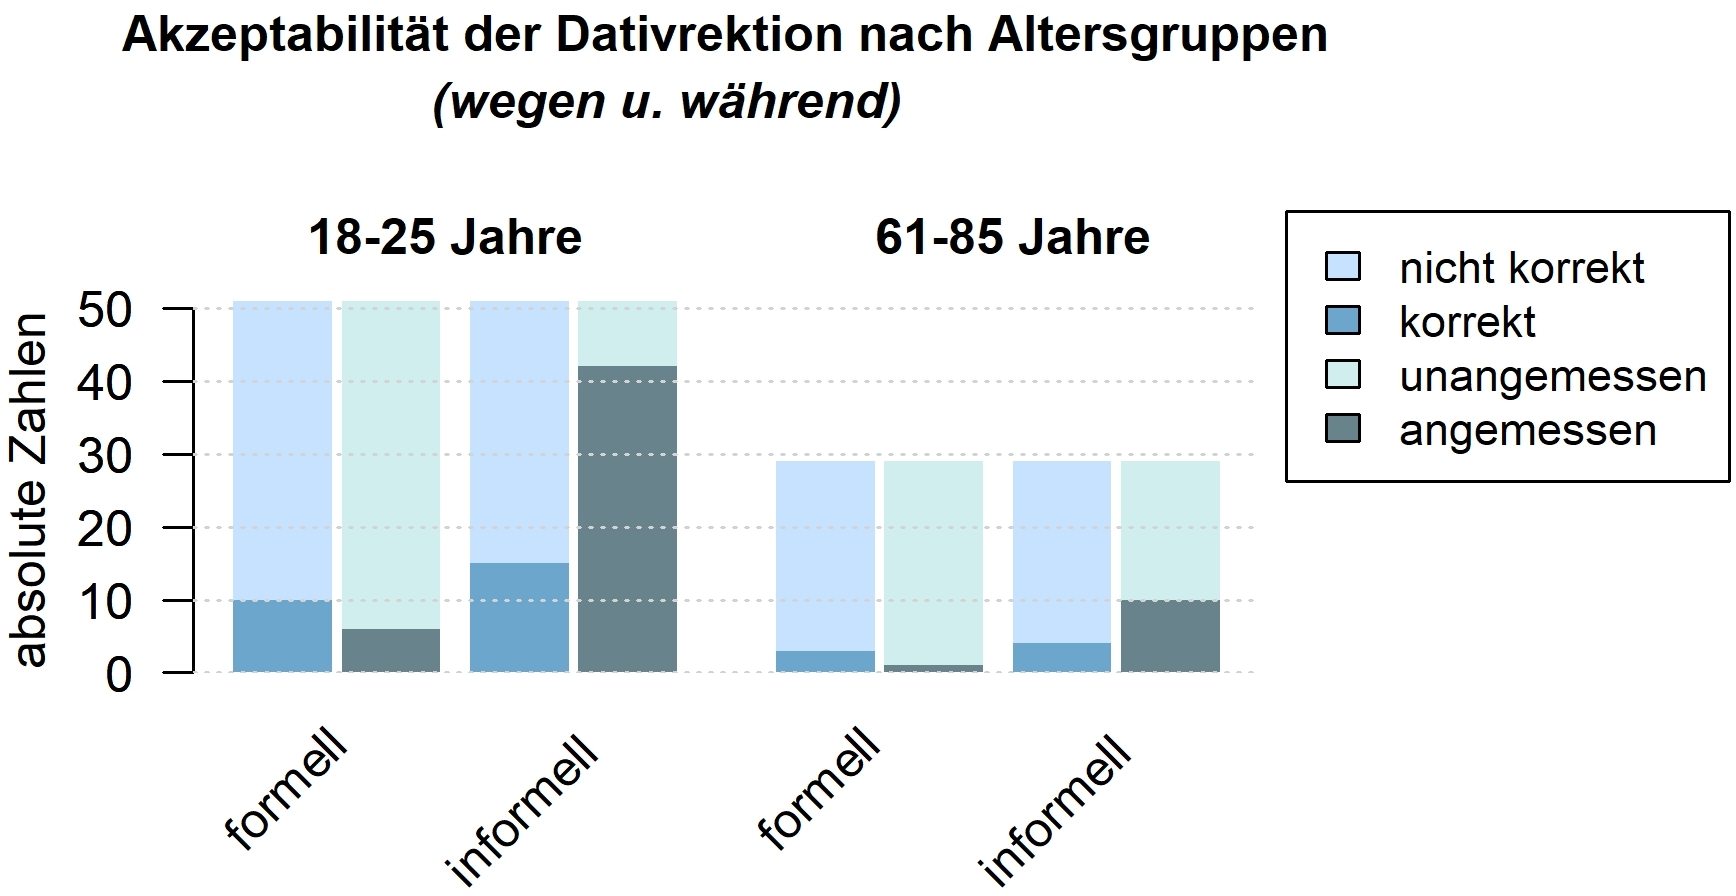
\includegraphics[scale=1]{AkzDativNachAlter.jpg}
%\caption{Akzeptabilität der Dativrektion bei \wegen{} und \waehrend{} nach Altersgruppen}
%\label{pic:AkzDativNachAlter}
%\end{figure}
%\begin{figure}
%\centering
%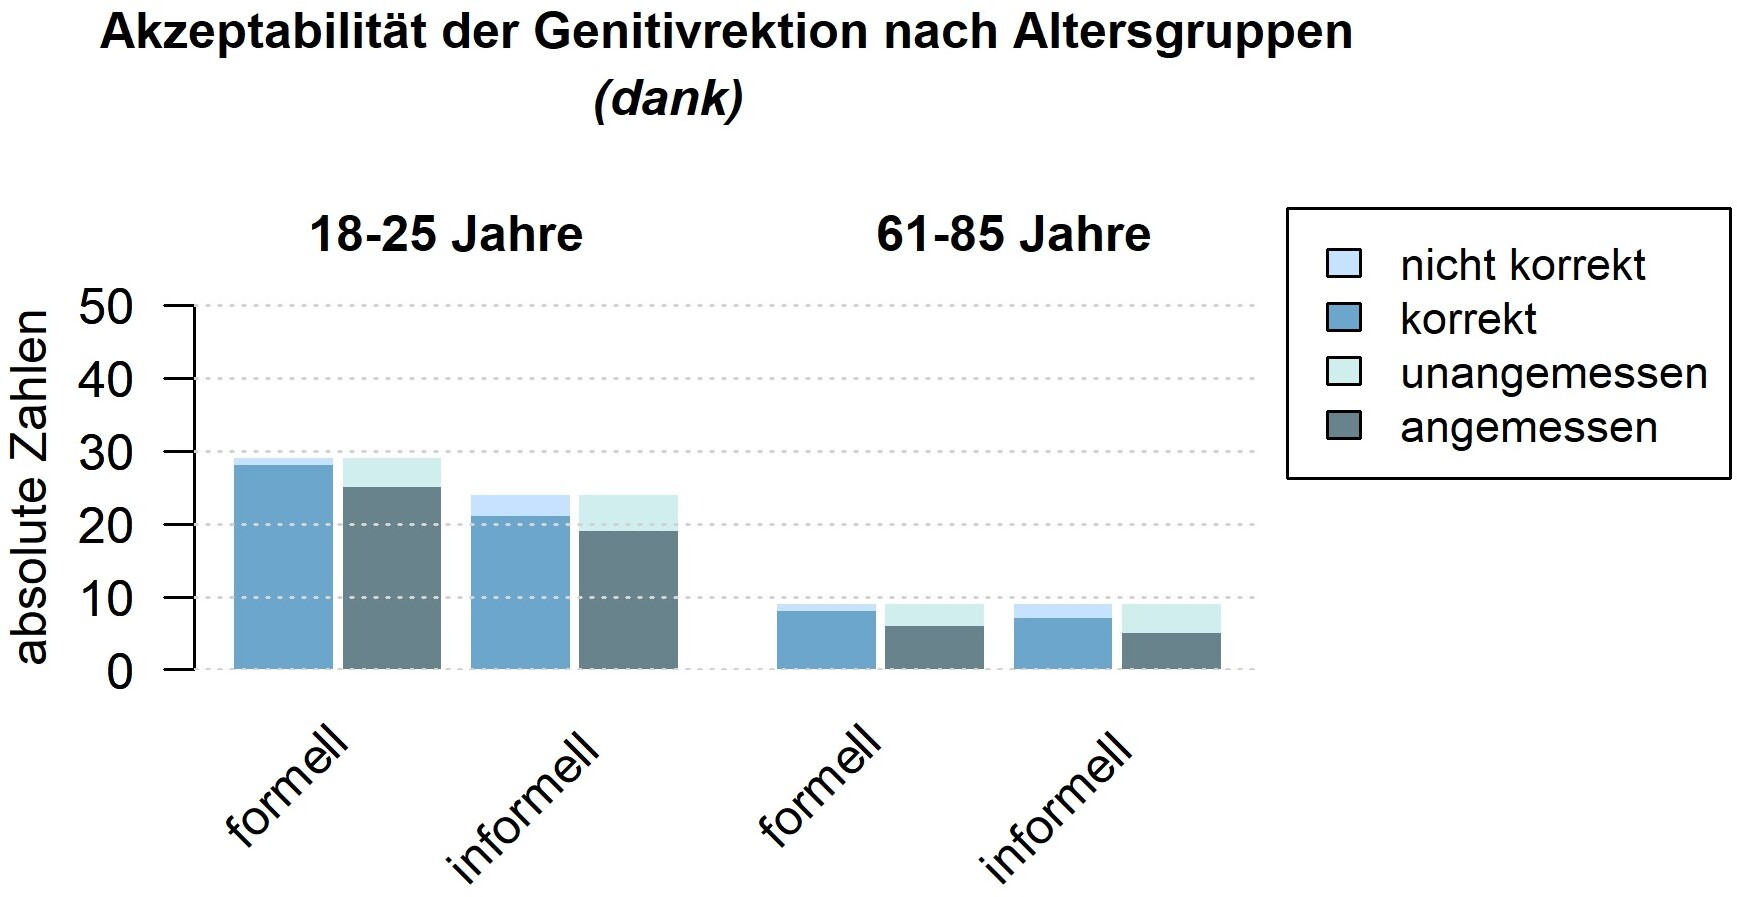
\includegraphics[scale=1]{AkzGenitivNachAlter.jpg}
%\caption{Akzeptabilität der Genitivrektion bei \dank{} nach Altersgruppen}
%\label{pic:AkzGenitivNachAlter}
%\end{figure}

Wie oben erläutert, bewerteten alle Befragten im Akzeptabilitätstest zusätzlich die Primärpräposition \object{seit} mit dem Genitiv. 
Abschließend werden daher die Akzeptabilitätswerte der Genitivrektion bei \object{seit} in den beiden Altersgruppen verglichen (s. \autoref{table:ErgAkzSeitNachAlter}).
In der Gruppe der 18- bis 25-Jährigen befinden sich insgesamt 104 Befragte, in der Gruppe der 61- bis 85-Jährigen 47. 
Im formellen Setting zeigen sich kaum Unterschiede zwischen den Altersgruppen.
Im informellen Setting bewerten unter den älteren Befragten jeweils weniger \object{seit} plus Genitiv als korrekt und angemessen. 
Dass sie die Form selbst verwenden würden, geben aus beiden Altersgruppen jedoch ähnlich viele an. 
% Please add the following required packages to your document preamble:
% \usepackage{multirow}
% \usepackage[table,xcdraw]{xcolor}
% If you use beamer only pass "xcolor=table" option, i.e. \documentclass[xcolor=table]{beamer}
\begin{table}
\centering
\begin{tabular}{llrrrr}
\multicolumn{6}{l}{\object{seit} + Genitiv nach Alter}                                                                                                                                                                                                                                            \\ \hline
                                                                                &                                      & \multicolumn{2}{c}{\begin{tabular}[c]{@{}c@{}}18--25 Jahre\\ (n=104)\end{tabular}} & \multicolumn{2}{c}{\begin{tabular}[c]{@{}c@{}}61--85 Jahre\\ (n=47)\end{tabular}} \\ \hline
                                                                                & \cellcolor[HTML]{9B9B9B}korrekt      & \cellcolor[HTML]{9B9B9B}32         & \cellcolor[HTML]{9B9B9B}{\footnotesize (30,77 \%)}        & \cellcolor[HTML]{9B9B9B}13         & \cellcolor[HTML]{9B9B9B}{\footnotesize (27,66 \%)}        \\ %\cline{2-6} 
                                                                                & \cellcolor[HTML]{9B9B9B}inkorrekt    & \cellcolor[HTML]{9B9B9B}72         & \cellcolor[HTML]{9B9B9B}{\footnotesize (69,23 \%)}        & \cellcolor[HTML]{9B9B9B}34         & \cellcolor[HTML]{9B9B9B}{\footnotesize (72,34 \%)}        \\ %\cline{2-6} 
                                                                                & \cellcolor[HTML]{EFEFEF}angemessen   & \cellcolor[HTML]{EFEFEF}32         & \cellcolor[HTML]{EFEFEF}{\footnotesize (30,77 \%)}        & \cellcolor[HTML]{EFEFEF}12         & \cellcolor[HTML]{EFEFEF}{\footnotesize (25,53 \%)}        \\ %\cline{2-6} 
                                                                                & \cellcolor[HTML]{EFEFEF}unangemessen & \cellcolor[HTML]{EFEFEF}72         & \cellcolor[HTML]{EFEFEF}{\footnotesize (69,23 \%)}        & \cellcolor[HTML]{EFEFEF}35         & \cellcolor[HTML]{EFEFEF}{\footnotesize (74,47 \%)}        \\ %\cline{2-6} 
                                                                                & eigene Verwendung ja                 & 27                                 & {\footnotesize (25,96 \%)}                                & 11                                 & {\footnotesize (23,4 \%)}                                 \\ %\cline{2-6} 
\multirow{-6}{*}{\begin{tabular}[c]{@{}l@{}}formelles\\ Setting\end{tabular}}   & eigene Verwendung nein               & 77                                 & {\footnotesize (74,04 \%)}                                & 36                                 & {\footnotesize (76,6 \%)}                                 \\ \hline
                                                                                &                                      & \multicolumn{2}{c}{\begin{tabular}[c]{@{}c@{}}18--25 Jahre\\ (n=104)\end{tabular}} & \multicolumn{2}{c}{\begin{tabular}[c]{@{}c@{}}61--85 Jahre\\ (n=47)\end{tabular}} \\ \hline
                                                                                & \cellcolor[HTML]{9B9B9B}korrekt      & \cellcolor[HTML]{9B9B9B}28         & \cellcolor[HTML]{9B9B9B}{\footnotesize (26,92 \%)}        & \cellcolor[HTML]{9B9B9B}7          & \cellcolor[HTML]{9B9B9B}{\footnotesize (14,89 \%)}        \\ %\cline{2-6} 
                                                                                & \cellcolor[HTML]{9B9B9B}inkorrekt    & \cellcolor[HTML]{9B9B9B}76         & \cellcolor[HTML]{9B9B9B}{\footnotesize (73,08 \%)}        & \cellcolor[HTML]{9B9B9B}40         & \cellcolor[HTML]{9B9B9B}{\footnotesize (85,11 \%)}        \\ %\cline{2-6} 
                                                                                & \cellcolor[HTML]{EFEFEF}angemessen   & \cellcolor[HTML]{EFEFEF}27         & \cellcolor[HTML]{EFEFEF}{\footnotesize (25,96 \%)}        & \cellcolor[HTML]{EFEFEF}7          & \cellcolor[HTML]{EFEFEF}{\footnotesize (14,89 \%)}        \\ %\cline{2-6} 
                                                                                & \cellcolor[HTML]{EFEFEF}unangemessen & \cellcolor[HTML]{EFEFEF}77         & \cellcolor[HTML]{EFEFEF}{\footnotesize (74,04 \%)}        & \cellcolor[HTML]{EFEFEF}40         & \cellcolor[HTML]{EFEFEF}{\footnotesize (85,11 \%)}        \\ %\cline{2-6} 
                                                                                & eigene Verwendung ja                 & 12                                 & {\footnotesize (11,54 \%)}                                & 7                                  & {\footnotesize (14,89 \%)}                                \\ %\cline{2-6} 
\multirow{-6}{*}{\begin{tabular}[c]{@{}l@{}}informelles\\ Setting\end{tabular}} & eigene Verwendung nein               & 92                                 & {\footnotesize (88,46 \%)}                               & 40                                 & {\footnotesize (85,11 \%)}                                \\ \hline
\end{tabular}
\caption{Akzeptabilität der Genitivrektion bei \object{seit} nach Alter}
\label{table:ErgAkzSeitNachAlter}
\end{table}

Der Vergleich der beiden Altersgruppen deutet darauf hin, dass ältere und jüngere SprachbenutzerInnen die Dativrektion bei \wegen{} und \waehrend{} und die Genitivrektion bei \dank{} ähnlich bewerten. 
In der Beurteilung der Angemessenheit im informellen Kontext zeigen sich aber jeweils Unterschiede, hier scheinen die Jüngeren offener gegenüber dem Dativ zu sein. 
Bei \wegen{} und \waehrend{} geben sie auch häufiger an, die Dativrektion in einem informellen Kontext selbst zu verwenden. 
Dass die älteren Befragten den Dativ bei \wegen{}, \waehrend{} und \dank{} weniger zu akzeptieren scheinen, könnte jedoch dadurch bedingt sein, dass in dieser Gruppe deutlich mehr Norddeutsche sind. 
Bei \gegenueber{} plus Genitiv deuten sich Unterschiede im formellen Setting an:
Während ca. die Hälfte der jüngeren Befragten die Variante akzeptiert, wird sie von beinahe allen älteren Befragten abgelehnt. 
Aufgrund der geringen Stichprobengröße kann es sich allerdings auch um zufällige Unterschiede handeln. 
Die Genitivrektion bei der Primärpräposition \object{seit} wird im informellen Kontext von der älteren Befragtengruppe etwas seltener als korrekt und angemessen bewertet als von der jüngeren. 
\subsection{Akzeptabilität und regionale Herkunft}
\label{sec:ErgAkzNachRegion}
% Akzeptabilität und regionale Herkunft
Die in \autoref{sec:KorpusstudienRektion} vorgestellten Korpusstudien zur regionalen Verteilung der Rektionsvarianten lassen vermuten, dass der Dativ in süddeutschen Bundesländern akzeptierter ist als in norddeutschen. 
Dies soll nun anhand der Daten aus dem Akzeptabilitätstest überprüft werden. 
Hierfür werden die Befragten aus norddeutschen Bundesländern (Bremen, Hamburg, Niedersachsen und Schleswig-Holstein) den Befragten aus süddeutschen Bundesländern (Bayern oder Baden-Württemberg) gegenübergestellt. 
Dabei ist zu berücksichtigen, dass unter den norddeutschen Befragten der Anteil von Personen über 60 deutlich höher ist (22~\%) als unter den süddeutschen Befragten (3~\%, s. \autoref{sec:HerkunftundDialekt}). 
Wieder werden zunächst \wegen{} und \waehrend{} gemeinsam betrachtet, anschließend \dank{}, \gegenueber{} und \object{seit} jeweils einzeln. 

\autoref{table:ErgAkzDativNachHerkunft} zeigt die summierten Akzeptabilitätswerte für \wegen{} und \waehrend{} mit dem Dativ, aufgeteilt nach regionaler Herkunft. 
Insgesamt wurden die beiden ursprünglichen Genitivpräpositionen von 81 Befragten aus Norddeutschland und 46 Befragten aus Süddeutschland bewertet. 
Diese regionalen Gruppen setzen sich wie folgt zusammen: 
Von den 81 norddeutschen Befragten sind 41 in der Gruppe, die die Akzeptabilität von \wegen{} plus Dativ im formellen und diejenige von \waehrend{} plus Dativ im informellen Kontext bewertete.
40 Norddeutsche erhielten umgekehrt \waehrend{} im formellen und \wegen{} im informellen Kontext zur Beurteilung. 
Von den 46 süddeutschen Befragten finden sich in der ersten Gruppe 19 und in der zweiten Gruppe 27. 
% Please add the following required packages to your document preamble:
% \usepackage{multirow}
% \usepackage[table,xcdraw]{xcolor}
% If you use beamer only pass "xcolor=table" option, i.e. \documentclass[xcolor=table]{beamer}
\begin{table}
\centering
\begin{tabular}{llrrrr}
\multicolumn{6}{l}{\wegen{} oder \waehrend{} + Dativ nach regionaler Herkunft}                                                                                                                                                                                                                                 \\ \hline
                                                                                &                                      & \multicolumn{2}{c}{\begin{tabular}[c]{@{}c@{}}Norddeutschland\\ (n=81)\end{tabular}} & \multicolumn{2}{c}{\begin{tabular}[c]{@{}c@{}}Süddeutschland\\ (n=46)\end{tabular}} \\ \hline
                                                                                & \cellcolor[HTML]{9B9B9B}korrekt      & \cellcolor[HTML]{9B9B9B}13            & \cellcolor[HTML]{9B9B9B}{\footnotesize (16,05 \%)}           & \cellcolor[HTML]{9B9B9B}13           & \cellcolor[HTML]{9B9B9B}{\footnotesize (28,26 \%)}           \\ %\cline{2-6} 
                                                                                & \cellcolor[HTML]{9B9B9B}inkorrekt    & \cellcolor[HTML]{9B9B9B}68            & \cellcolor[HTML]{9B9B9B}{\footnotesize (83,95 \%)}           & \cellcolor[HTML]{9B9B9B}33           & \cellcolor[HTML]{9B9B9B}{\footnotesize (71,74 \%)}           \\ %\cline{2-6} 
                                                                                & \cellcolor[HTML]{EFEFEF}angemessen   & \cellcolor[HTML]{EFEFEF}8             & \cellcolor[HTML]{EFEFEF}{\footnotesize (9,88 \%)}            & \cellcolor[HTML]{EFEFEF}6            & \cellcolor[HTML]{EFEFEF}{\footnotesize (13,04 \%)}           \\ %\cline{2-6} 
                                                                                & \cellcolor[HTML]{EFEFEF}unangemessen & \cellcolor[HTML]{EFEFEF}73            & \cellcolor[HTML]{EFEFEF}{\footnotesize (90,12 \%)}           & \cellcolor[HTML]{EFEFEF}40           & \cellcolor[HTML]{EFEFEF}{\footnotesize (86,96 \%)}           \\ %\cline{2-6} 
                                                                                & eigene Verwendung ja                 & 5                                     & {\footnotesize (6,17 \%)}                                    & 8                                    & {\footnotesize (17,39 \%)}                                   \\ %\cline{2-6} 
\multirow{-6}{*}{\begin{tabular}[c]{@{}l@{}}formelles\\ Setting\end{tabular}}   & eigene Verwendung nein               & 76                                    & {\footnotesize (93,83 \%)}                                   & 38                                   & {\footnotesize (82,61 \%)}                                   \\ \hline
                                                                                &                                      & \multicolumn{2}{c}{\begin{tabular}[c]{@{}c@{}}Norddeutschland\\ (n=81)\end{tabular}} & \multicolumn{2}{c}{\begin{tabular}[c]{@{}c@{}}Süddeutschland\\ (n=46)\end{tabular}} \\ \hline
                                                                                & \cellcolor[HTML]{9B9B9B}korrekt      & \cellcolor[HTML]{9B9B9B}11            & \cellcolor[HTML]{9B9B9B}{\footnotesize (13,58 \%)}           & \cellcolor[HTML]{9B9B9B}22           & \cellcolor[HTML]{9B9B9B}{\footnotesize (47,83 \%)}           \\ %\cline{2-6} 
                                                                                & \cellcolor[HTML]{9B9B9B}inkorrekt    & \cellcolor[HTML]{9B9B9B}70            & \cellcolor[HTML]{9B9B9B}{\footnotesize (86,42 \%)}           & \cellcolor[HTML]{9B9B9B}24           & \cellcolor[HTML]{9B9B9B}{\footnotesize (52,17 \%)}           \\ %\cline{2-6} 
                                                                                & \cellcolor[HTML]{EFEFEF}angemessen   & \cellcolor[HTML]{EFEFEF}39            & \cellcolor[HTML]{EFEFEF}{\footnotesize (48,15 \%)}           & \cellcolor[HTML]{EFEFEF}41           & \cellcolor[HTML]{EFEFEF}{\footnotesize (89,13 \%)}           \\ %\cline{2-6} 
                                                                                & \cellcolor[HTML]{EFEFEF}unangemessen & \cellcolor[HTML]{EFEFEF}42            & \cellcolor[HTML]{EFEFEF}{\footnotesize (51,85 \%)}           & \cellcolor[HTML]{EFEFEF}5            & \cellcolor[HTML]{EFEFEF}{\footnotesize (10,87 \%)}           \\ %\cline{2-6} 
                                                                                & eigene Verwendung ja                 & 22                                    & {\footnotesize (27,16 \%)}                                   & 38                                   & {\footnotesize (82,61 \%)}                                   \\ %\cline{2-6} 
\multirow{-6}{*}{\begin{tabular}[c]{@{}l@{}}informelles\\ Setting\end{tabular}} & eigene Verwendung nein               & 59                                    & {\footnotesize (72,84 \%)}                                   & 8                                    & {\footnotesize (17,39 \%)}                                   \\ \hline
\end{tabular}
\caption{Akzeptabilität der Dativrektion bei \wegen{} oder \waehrend{} nach regionaler Herkunft}
\label{table:ErgAkzDativNachHerkunft}
\end{table}

Im informellen Kontext akzeptieren die süddeutschen BefragungsteilnehmerInnen den Dativ eher als die norddeutschen. 
Ungefähr die Hälfte der 46 Befragten aus Süddeutschland beurteilt die Dativrektion bei \wegen{} oder \waehrend{} als korrekt, im Norden tun dies hingegen nur elf von 81. 
Nur fünf Befragte aus Süddeutschland bewerten den Dativ im informellen Setting als unangemessen, acht würden ihn selbst nicht verwenden. 
Im Norden hingegen wird die Dativrektion bei \wegen{} oder \waehrend{} in einem informellen Kontext nur von ca. der Hälfte als angemessen empfunden (39 von 81) und nur ca. ein Viertel würde sie selbst verwenden. 
 Die Gruppe, die im Akzeptabilitätstest \dank{} mit dem Genitiv im formellen Setting beurteilt und \gegenueber{} mit dem Genitiv im informellen, umfasst 42 Befragte aus Norddeutschland und 27 Befragte aus Süddeutschland (s. \autoref{table:ErgAkzDankNachHerkunft} und \autoref{table:ErgAkzGegenueberNachHerkunft}).
49 Norddeutsche und 27 Süddeutsche bewerteten \dank{} im informellen und \gegenueber{} im formellen Setting. 
Beide ursprünglichen Dativpräpositionen werden auch hier wieder getrennt behandelt. 
% Please add the following required packages to your document preamble:
% \usepackage{multirow}
% \usepackage[table,xcdraw]{xcolor}
% If you use beamer only pass "xcolor=table" option, i.e. \documentclass[xcolor=table]{beamer}
\begin{table}
\centering
\begin{tabular}{llrrrr}
\multicolumn{6}{l}{\dank{} + Genitiv nach regionaler Herkunft}                                                                                                                                                                                                                                \\ \hline
                                                                                &                                      & \multicolumn{2}{c}{\begin{tabular}[c]{@{}c@{}}Norddeutschland\\ (n=42)\end{tabular}} & \multicolumn{2}{c}{\begin{tabular}[c]{@{}c@{}}Süddeutschland\\ (n=27)\end{tabular}} \\ \hline
                                                                                & \cellcolor[HTML]{9B9B9B}korrekt      & \cellcolor[HTML]{9B9B9B}37            & \cellcolor[HTML]{9B9B9B}{\footnotesize (88,1 \%)}            & \cellcolor[HTML]{9B9B9B}26           & \cellcolor[HTML]{9B9B9B}{\footnotesize (96,3 \%)}            \\ %\cline{2-6} 
                                                                                & \cellcolor[HTML]{9B9B9B}inkorrekt    & \cellcolor[HTML]{9B9B9B}5             & \cellcolor[HTML]{9B9B9B}{\footnotesize (11,9 \%})            & \cellcolor[HTML]{9B9B9B}1            & \cellcolor[HTML]{9B9B9B}{\footnotesize (3,7 \%})             \\ %\cline{2-6} 
                                                                                & \cellcolor[HTML]{EFEFEF}angemessen   & \cellcolor[HTML]{EFEFEF}32            & \cellcolor[HTML]{EFEFEF}{\footnotesize (76,19 \%)}           & \cellcolor[HTML]{EFEFEF}23           & \cellcolor[HTML]{EFEFEF}{\footnotesize (85,19 \%)}           \\ %\cline{2-6} 
                                                                                & \cellcolor[HTML]{EFEFEF}unangemessen & \cellcolor[HTML]{EFEFEF}10            & \cellcolor[HTML]{EFEFEF}{\footnotesize (23,81 \%)}           & \cellcolor[HTML]{EFEFEF}4            & \cellcolor[HTML]{EFEFEF}{\footnotesize (14,81 \%)}           \\ %\cline{2-6} 
                                                                                & eigene Verwendung ja                 & 26                                    & {\footnotesize (61,9 \%)}                                    & 22                                   & {\footnotesize (81,48 \%)}                                   \\ %\cline{2-6} 
\multirow{-6}{*}{\begin{tabular}[c]{@{}l@{}}formelles\\ Setting\end{tabular}}   & eigene Verwendung nein               & 16                                    & {\footnotesize (38,1 \%)}                                    & 5                                    & {\footnotesize (18,52 \%)}                                   \\ \hline
                                                                                &                                      & \multicolumn{2}{c}{\begin{tabular}[c]{@{}c@{}}Norddeutschland\\ (n=49)\end{tabular}} & \multicolumn{2}{c}{\begin{tabular}[c]{@{}c@{}}Süddeutschland\\ (n=27)\end{tabular}} \\ \hline
                                                                                & \cellcolor[HTML]{9B9B9B}korrekt      & \cellcolor[HTML]{9B9B9B}47            & \cellcolor[HTML]{9B9B9B}{\footnotesize (95,92 \%)}           & \cellcolor[HTML]{9B9B9B}26           & \cellcolor[HTML]{9B9B9B}{\footnotesize (96,3 \%)}            \\ %\cline{2-6} 
                                                                                & \cellcolor[HTML]{9B9B9B}inkorrekt    & \cellcolor[HTML]{9B9B9B}2             & \cellcolor[HTML]{9B9B9B}{\footnotesize (4,08 \%)}            & \cellcolor[HTML]{9B9B9B}1            & \cellcolor[HTML]{9B9B9B}{\footnotesize (3,7 \%)}             \\ %\cline{2-6} 
                                                                                & \cellcolor[HTML]{EFEFEF}angemessen   & \cellcolor[HTML]{EFEFEF}38            & \cellcolor[HTML]{EFEFEF}{\footnotesize (77,55 \%)}           & \cellcolor[HTML]{EFEFEF}20           & \cellcolor[HTML]{EFEFEF}{\footnotesize (74,07 \%)}           \\ %\cline{2-6} 
                                                                                & \cellcolor[HTML]{EFEFEF}unangemessen & \cellcolor[HTML]{EFEFEF}11            & \cellcolor[HTML]{EFEFEF}{\footnotesize (22,45 \%)}           & \cellcolor[HTML]{EFEFEF}7            & \cellcolor[HTML]{EFEFEF}{\footnotesize (25,93 \%)}           \\ %\cline{2-6} 
                                                                                & eigene Verwendung ja                 & 38                                    & {\footnotesize (77,55 \%)}                                   & 16                                   & {\footnotesize (59,26 \%)}                                   \\ %\cline{2-6} 
\multirow{-6}{*}{\begin{tabular}[c]{@{}l@{}}informelles\\ Setting\end{tabular}} & eigene Verwendung nein               & 11                                    & {\footnotesize (22,45 \%)}                                   & 11                                   & {\footnotesize (40,74 \%)}                                   \\ \hline
\end{tabular}
\caption{Akzeptabilität der Genitivrektion bei \dank{} nach regionaler Herkunft}
\label{table:ErgAkzDankNachHerkunft}
\end{table}

Die Korrektheit und die Angemessenheit der Genitivrektion bei \dank{} bewerten norddeutsche und süddeutsche Befragte recht ähnlich.
Unterschiede zeigen sich aber in den Angaben zur eigenen Verwendung: 
Im formellen Setting ist der Anteil derer, die \dank{} plus Genitiv verwenden würden, in Süddeutschland deutlich höher als in Norddeutschland. 
Im informellen Setting ist es umgekehrt: Hier würden nur 16 von 27 Befragten aus Süddeutschland den Genitiv verwenden, jedoch 38 von 49 norddeutschen Befragten. 

Die Genitivrektion bei \gegenueber{} wird im informellen Setting von süddeutschen Befragten recht häufig akzeptiert (s. \autoref{table:ErgAkzGegenueberNachHerkunft}): 
Ungefähr die Hälfte (jeweils 13 von 27) stuft \gegenueber{} plus Genitiv in einem Gespräch mit einem Freund als korrekt und angemessen ein. 
Unter den norddeutschen Befragten ist der Anteil deutlich geringer (neun bzw. 14 von 42). 
% Please add the following required packages to your document preamble:
% \usepackage{multirow}
% \usepackage[table,xcdraw]{xcolor}
% If you use beamer only pass "xcolor=table" option, i.e. \documentclass[xcolor=table]{beamer}
\begin{table}
\centering
\begin{tabular}{llrrrr}
\multicolumn{6}{l}{\gegenueber{} + Genitiv nach regionaler Herkunft}                                                                                                                                                                                                                          \\ \hline
                                                                                &                                      & \multicolumn{2}{c}{\begin{tabular}[c]{@{}c@{}}Norddeutschland\\ (n=49)\end{tabular}} & \multicolumn{2}{c}{\begin{tabular}[c]{@{}c@{}}Süddeutschland\\ (n=27)\end{tabular}} \\ \hline
                                                                                & \cellcolor[HTML]{9B9B9B}korrekt      & \cellcolor[HTML]{9B9B9B}19            & \cellcolor[HTML]{9B9B9B}{\footnotesize (38,78 \%)}           & \cellcolor[HTML]{9B9B9B}8            & \cellcolor[HTML]{9B9B9B}{\footnotesize (29,63 \%)}           \\ %\cline{2-6} 
                                                                                & \cellcolor[HTML]{9B9B9B}inkorrekt    & \cellcolor[HTML]{9B9B9B}30            & \cellcolor[HTML]{9B9B9B}{\footnotesize (61,22 \%})           & \cellcolor[HTML]{9B9B9B}19           & \cellcolor[HTML]{9B9B9B}{\footnotesize (70,37 \%)}           \\ %\cline{2-6} 
                                                                                & \cellcolor[HTML]{EFEFEF}angemessen   & \cellcolor[HTML]{EFEFEF}18            & \cellcolor[HTML]{EFEFEF}{\footnotesize (36,73 \%)}           & \cellcolor[HTML]{EFEFEF}9            & \cellcolor[HTML]{EFEFEF}{\footnotesize (33,33 \%)}           \\ %\cline{2-6} 
                                                                                & \cellcolor[HTML]{EFEFEF}unangemessen & \cellcolor[HTML]{EFEFEF}31            & \cellcolor[HTML]{EFEFEF}{\footnotesize (63,27 \%)}           & \cellcolor[HTML]{EFEFEF}18           & \cellcolor[HTML]{EFEFEF}{\footnotesize (66,67 \%)}           \\ %\cline{2-6} 
                                                                                & eigene Verwendung ja                 & 14                                    & {\footnotesize (28,57 \%)}                                   & 8                                    & {\footnotesize (29,63 \%)}                                   \\ %\cline{2-6} 
\multirow{-6}{*}{\begin{tabular}[c]{@{}l@{}}formelles\\ Setting\end{tabular}}   & eigene Verwendung nein               & 35                                    & {\footnotesize (71,43 \%)}                                   & 19                                   & {\footnotesize (70,37 \%)}                                   \\ \hline
                                                                                &                                      & \multicolumn{2}{c}{\begin{tabular}[c]{@{}c@{}}Norddeutschland\\ (n=42)\end{tabular}} & \multicolumn{2}{c}{\begin{tabular}[c]{@{}c@{}}Süddeutschland\\ (n=27)\end{tabular}} \\ \hline
                                                                                & \cellcolor[HTML]{9B9B9B}korrekt      & \cellcolor[HTML]{9B9B9B}9             & \cellcolor[HTML]{9B9B9B}{\footnotesize (21,43 \%)}           & \cellcolor[HTML]{9B9B9B}13           & \cellcolor[HTML]{9B9B9B}{\footnotesize (48,15 \%)}           \\ %\cline{2-6} 
                                                                                & \cellcolor[HTML]{9B9B9B}inkorrekt    & \cellcolor[HTML]{9B9B9B}33            & \cellcolor[HTML]{9B9B9B}{\footnotesize (78,57 \%)}           & \cellcolor[HTML]{9B9B9B}14           & \cellcolor[HTML]{9B9B9B}{\footnotesize (51,85 \%)}           \\ %\cline{2-6} 
                                                                                & \cellcolor[HTML]{EFEFEF}angemessen   & \cellcolor[HTML]{EFEFEF}14            & \cellcolor[HTML]{EFEFEF}{\footnotesize (33,33 \%)}           & \cellcolor[HTML]{EFEFEF}13           & \cellcolor[HTML]{EFEFEF}{\footnotesize (48,15 \%)}           \\ %\cline{2-6} 
                                                                                & \cellcolor[HTML]{EFEFEF}unangemessen & \cellcolor[HTML]{EFEFEF}28            & \cellcolor[HTML]{EFEFEF}{\footnotesize (66,67 \%)}           & \cellcolor[HTML]{EFEFEF}14           & \cellcolor[HTML]{EFEFEF}{\footnotesize (51,85 \%)}           \\ %\cline{2-6} 
                                                                                & eigene Verwendung ja                 & 8                                     & {\footnotesize (19,05 \%)}                                   & 8                                    & {\footnotesize (29,63 \%)}                                   \\ %\cline{2-6} 
\multirow{-6}{*}{\begin{tabular}[c]{@{}l@{}}informelles\\ Setting\end{tabular}} & eigene Verwendung nein               & 34                                    & {\footnotesize (80,95 \%)}                                   & 19                                   & {\footnotesize (70,37 \%)}                                   \\ \hline
\end{tabular}
\caption{Akzeptabilität der Genitivrektion bei \gegenueber{} nach regionaler Herkunft}
\label{table:ErgAkzGegenueberNachHerkunft}
\end{table}
%\begin{figure}
%\centering
%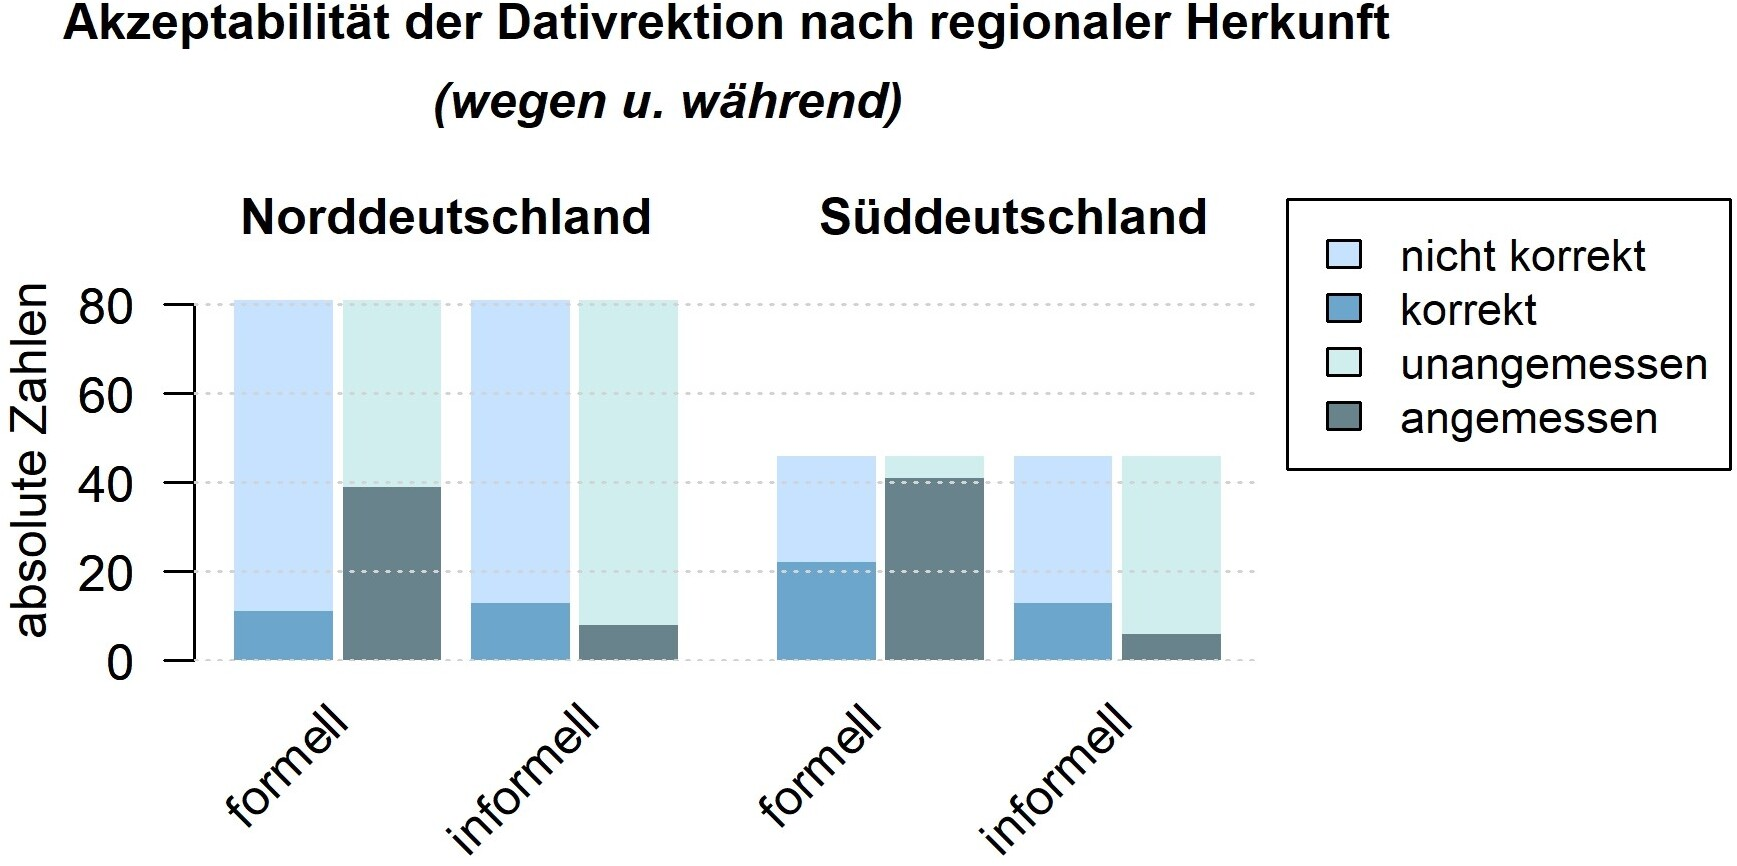
\includegraphics[scale=1]{AkzDativNachRegion.jpg}
%\caption{Akzeptabilität der Dativrektion bei \wegen{} und \waehrend{} nach regionaler Herkunft}
%\label{pic:AkzDativNachRegion}
%\end{figure}
%\begin{figure}
%\centering
%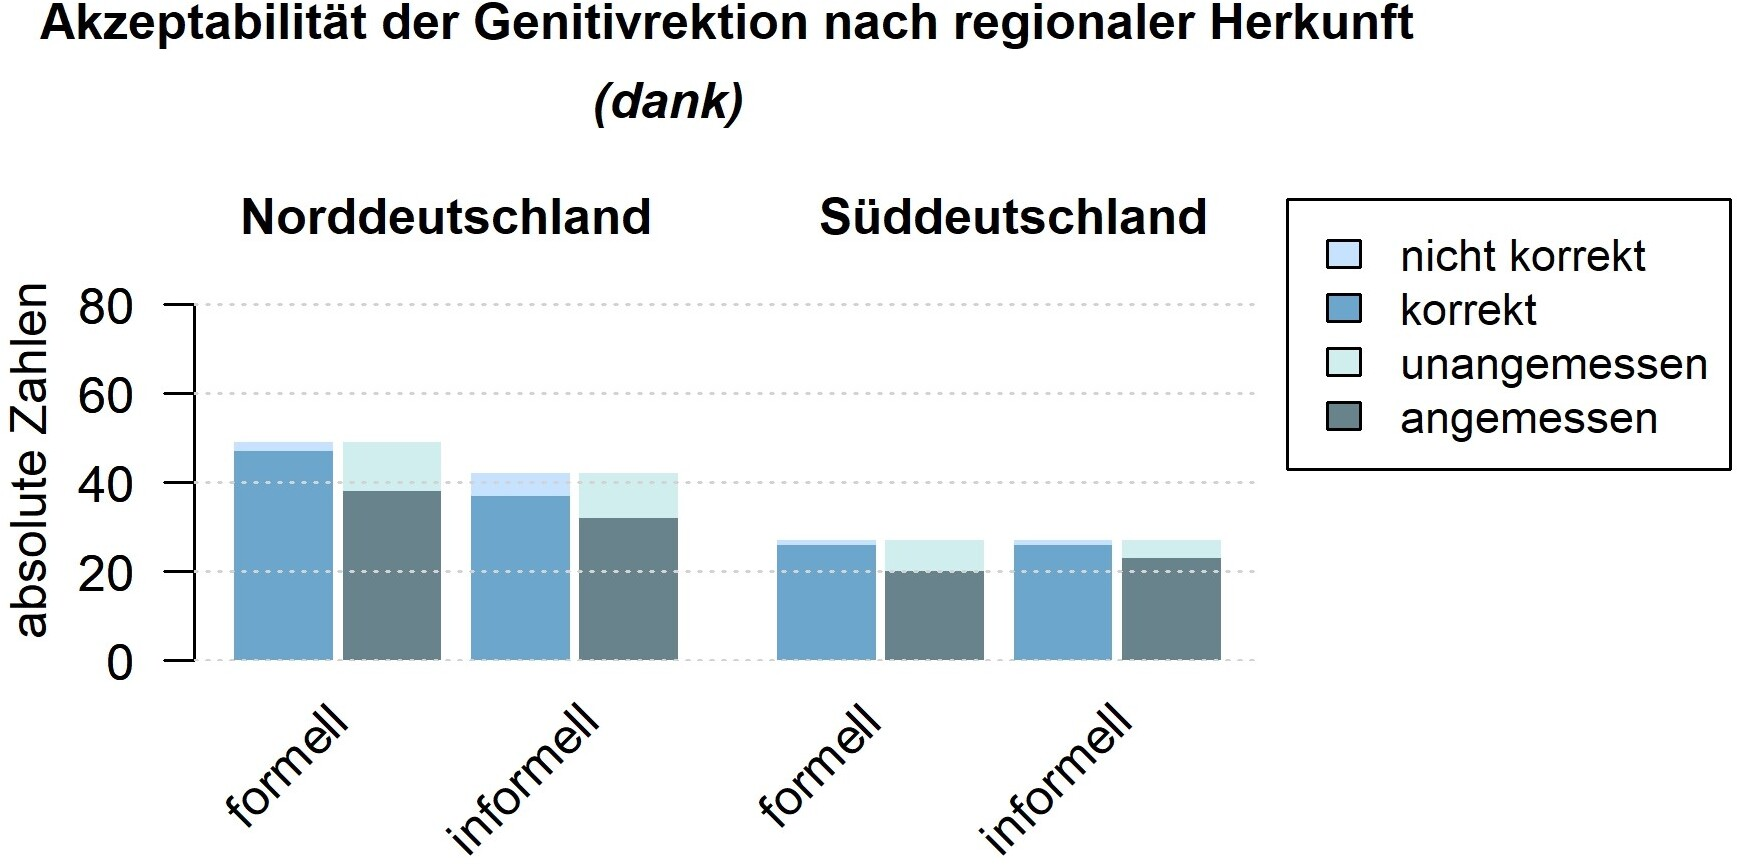
\includegraphics[scale=1]{AkzGenitivNachRegion.jpg}
%\caption{Akzeptabilität der Genitivrektion bei \dank{} nach regionaler Herkunft}
%\label{pic:AkzGenitivNachRegion}
%\end{figure}
% Please add the following required packages to your document preamble:
% \usepackage{multirow}
% \usepackage[table,xcdraw]{xcolor}
% If you use beamer only pass "xcolor=table" option, i.e. \documentclass[xcolor=table]{beamer}

Die Akzeptabilitätswerte der Genitivrektion bei der Primärpräposition \object{seit} sind im Norden (172 Befragte) und Süden (100 Befragte) ähnlich (s. \autoref{table:ErgAkzSeitNachHerkunft}).
Das gilt sowohl für das formelle als auch für das informelle Setting. 
Lediglich die Frage danach, ob sie die Variante selbst verwenden würden, wird unter den süddeutschen Befragten noch etwas häufiger verneint. 
\begin{table}
\centering
\begin{tabular}{llrrrr}
\multicolumn{6}{l}{\object{seit} + Genitiv nach regionaler Herkunft}                                                                                                                                                                                                                                  \\ \hline
                                                                                &                                      & \multicolumn{2}{c}{\begin{tabular}[c]{@{}c@{}}Norddeutschland\\ (n=172)\end{tabular}} & \multicolumn{2}{c}{\begin{tabular}[c]{@{}c@{}}Süddeutschland\\ (n=100)\end{tabular}} \\ \hline
                                                                                & \cellcolor[HTML]{9B9B9B}korrekt      & \cellcolor[HTML]{9B9B9B}61             & \cellcolor[HTML]{9B9B9B}{\footnotesize (35,47 \%)}           & \cellcolor[HTML]{9B9B9B}31             & \cellcolor[HTML]{9B9B9B}{\footnotesize (31 \%)}             \\ %\cline{2-6} 
                                                                                & \cellcolor[HTML]{9B9B9B}inkorrekt    & \cellcolor[HTML]{9B9B9B}111            & \cellcolor[HTML]{9B9B9B}{\footnotesize (64,53 \%)}           & \cellcolor[HTML]{9B9B9B}69             & \cellcolor[HTML]{9B9B9B}{\footnotesize (69 \%)}             \\ %\cline{2-6} 
                                                                                & \cellcolor[HTML]{EFEFEF}angemessen   & \cellcolor[HTML]{EFEFEF}64             & \cellcolor[HTML]{EFEFEF}{\footnotesize (37,21 \%)}           & \cellcolor[HTML]{EFEFEF}33             & \cellcolor[HTML]{EFEFEF}{\footnotesize (33 \%)}             \\ %\cline{2-6} 
                                                                                & \cellcolor[HTML]{EFEFEF}unangemessen & \cellcolor[HTML]{EFEFEF}108            & \cellcolor[HTML]{EFEFEF}{\footnotesize (62,79 \%)}           & \cellcolor[HTML]{EFEFEF}67             & \cellcolor[HTML]{EFEFEF}{\footnotesize (67 \%)}             \\ %\cline{2-6} 
                                                                                & eigene Verwendung ja                 & 56                                     & {\footnotesize (32,56 \%)}                                   & 23                                     & {\footnotesize (23 \%)}                                     \\ %\cline{2-6} 
\multirow{-6}{*}{\begin{tabular}[c]{@{}l@{}}formelles\\ Setting\end{tabular}}   & eigene Verwendung nein               & 116                                    & {\footnotesize (67,44 \%)}                                   & 77                                     & {\footnotesize (77 \%)                                  } \\ \hline
                                                                                &                                      & \multicolumn{2}{c}{\begin{tabular}[c]{@{}c@{}}Norddeutschland\\ (n=172)\end{tabular}} & \multicolumn{2}{c}{\begin{tabular}[c]{@{}c@{}}Süddeutschland\\ (n=100)\end{tabular}} \\ \hline
                                                                                & \cellcolor[HTML]{9B9B9B}korrekt      & \cellcolor[HTML]{9B9B9B}39             & \cellcolor[HTML]{9B9B9B}{\footnotesize (22,67 \%)}           & \cellcolor[HTML]{9B9B9B}21             & \cellcolor[HTML]{9B9B9B}{\footnotesize (21 \%)}             \\ %\cline{2-6} 
                                                                                & \cellcolor[HTML]{9B9B9B}inkorrekt    & \cellcolor[HTML]{9B9B9B}133            & \cellcolor[HTML]{9B9B9B}{\footnotesize (77,33 \%)}           & \cellcolor[HTML]{9B9B9B}79             & \cellcolor[HTML]{9B9B9B}{\footnotesize (79 \%)}             \\ %\cline{2-6} 
                                                                                & \cellcolor[HTML]{EFEFEF}angemessen   & \cellcolor[HTML]{EFEFEF}50             & \cellcolor[HTML]{EFEFEF}{\footnotesize (29,07 \%)}           & \cellcolor[HTML]{EFEFEF}21             & \cellcolor[HTML]{EFEFEF}{\footnotesize(21 \%)}             \\ %\cline{2-6} 
                                                                                & \cellcolor[HTML]{EFEFEF}unangemessen & \cellcolor[HTML]{EFEFEF}122            & \cellcolor[HTML]{EFEFEF}{\footnotesize (70,93 \%)}           & \cellcolor[HTML]{EFEFEF}79             & \cellcolor[HTML]{EFEFEF}{\footnotesize (79 \%)}             \\ %\cline{2-6} 
                                                                                & eigene Verwendung ja                 & 29                                     & {\footnotesize (16,86 \%)}                                   & 7                                      & {\footnotesize (7 \%)}                                      \\ %\cline{2-6} 
\multirow{-6}{*}{\begin{tabular}[c]{@{}l@{}}informelles\\ Setting\end{tabular}} & eigene Verwendung nein               & 143                                    & {\footnotesize (83,14 \%)}                                   & 93                                     & {\footnotesize (93 \%)}                                     \\ \hline
\end{tabular}
\caption{Akzeptabilität der Genitivrektion bei \object{seit} nach regionaler Herkunft}
\label{table:ErgAkzSeitNachHerkunft}
\end{table}

Zusammenfassend lässt sich festhalten, dass die Dativrektion im Süden etwas akzeptierter zu sein scheint. 
Die Ergebnisse zur Genitivrektion sind weniger klar, es zeigt sich aber bei \gegenueber{} plus Genitiv die Tendenz, dass die Variante in Süddeutschland eher akzeptiert wird. 
\subsection{Akzeptabilität und Bildungsstand}
\label{sec:ErgAkzNachBildung}
% Akzeptabilität nach Bildungsstand
Wie die Auswertung der freien Assoziationen gezeigt hat, ist Bildung eine besonders wichtige Kategorie bei der Konzeptualisierung der Rektionsvarianten von Sekundärpräpositionen (\autoref{sec:ErgAssPersonen}). 
Daher wird im Folgenden überprüft, ob der Bildungsgrad der Befragten ihre Bewertung der Rektionskasus beeinflusst. 
Da der Genitiv indexikalisch für hohe Bildung steht, ist einerseits denkbar, dass Befragte mit niedrigem Bildungsstand diesen Kasus besonders positiv bewerten, um sich selbst als gebildet zu positionieren. 
Andererseits könnte die Genitivrektion von Befragten mit niedrigem Bildungsstand als Verweis auf eine Gruppe gedeutet werden, von der sie sich abgrenzen möchten, und daher negativer bewertet werden. 

Für die Untersuchung des Zusammenhangs zwischen Akzeptabilität und Bildung werden die Befragten in zwei Bildungsgruppen geteilt: Befragte mit Hochschulabschluss (insgesamt 267) und Befragte ohne Hochschulabschluss (insgesamt 130). 
Die Gruppe der Befragten mit Hochschulabschluss umfasst alle Befragten, die im Fragebogen als höchsten Bildungsstand \glqq Hochschulabschluss\grqq{} oder \glqq Promotion/Habilitation\grqq{} angeben, sowie die Befragten, die unter \glqq anderer Abschluss\grqq{} \glqq Staatsexamen\grqq{} oder \glqq Diplom\grqq{} angeben (\autoref{sec:Bildung}). 
Die Gruppe der Befragten ohne Hochschulabschluss besteht aus Befragten, die als höchsten Abschluss \glqq Hauptschul-/Realschulabschluss\grqq{} oder \glqq Abitur/Fachabitur\grqq{} angeben sowie einem Befragten, der als anderen Abschluss \glqq Industriemeister\grqq{} nennt. 
In \autoref{sec:Bildung} und in \autoref{sec:ErgAkzNachAlter} wurde bereits auf die Heterogenität innerhalb der Gruppe ohne Hochschulabschluss hingewiesen:
Zum einen befinden sich in dieser Gruppe Befragte ohne Abitur.  Diese gehören größtenteils zu den älteren Befragten; von den insgesamt 37 Befragten ohne Abitur sind 14 über 60. 
Zum anderen befinden sich in der Gruppe ohne Hochschulabschluss viele unter 26-jährige Befragte mit Abitur, deren Hochschulstudium noch nicht abgeschlossen ist. 
Dies muss bei der Betrachtung der beiden Bildungsgruppen berücksichtigt werden. 

Wie bereits beim Vergleich der Altersgruppen und Herkunftsregionen werden auch für den Vergleich von Befragten mit unterschiedlichem Bildungsstand zunächst die Akzeptabilitätswerte von \wegen{} und \waehrend{} mit der Dativrektion zusammen betrachtet und anschließend jeweils einzeln die Akzeptabilitätswerte von \dank{}, \gegenueber{} und \object{seit}.

In der Gruppe, die \wegen{} plus Dativ im formellen Setting und \waehrend{} plus Dativ im informellen Setting bewertete, sind 73 Personen mit Hochschulabschluss und 28 Personen ohne Hochschulabschluss (s. \autoref{table:ErgAkzDativNachBildung}). 
Unter den Befragten, die \wegen{} plus Dativ im informellen und \waehrend{} plus Dativ im formellen Setting bewerten, sind 58 mit und 38 ohne Hochschulabschluss. 
Insgesamt bewerteten also 131 Befragte mit Hochschulabschluss die Dativrektion und 66 Befragte ohne Hochschulabschluss. 
%% Please add the following required packages to your document preamble:
%% \usepackage{multirow}
%% \usepackage[table,xcdraw]{xcolor}
%% If you use beamer only pass "xcolor=table" option, i.e. \documentclass[xcolor=table]{beamer}
%\begin{table}
%\centering
%\begin{tabular}{llrr}
%\multicolumn{4}{l}{\textbf{\wegen{} und \waehrend{} + Dativ nach Bildungsstand}}                                                                                                                                                                                               \\ \hline
%\multicolumn{1}{c}{}                  &                                      & \multicolumn{1}{c}{\begin{tabular}[c]{@{}c@{}}Hochschulabschluss\\ (n = 131)\end{tabular}} & \multicolumn{1}{c}{\begin{tabular}[c]{@{}c@{}}kein\\ Hochschulabschluss\\ (n = 66)\end{tabular}} \\ \hline
%                                      & \cellcolor[HTML]{9B9B9B}korrekt      & \cellcolor[HTML]{9B9B9B}\begin{tabular}[c]{@{}r@{}}20\\ {\small (xx \%)}\end{tabular}}                                                                 & \cellcolor[HTML]{9B9B9B}12                                                                     \\ %\cline{2-4} 
%                                      & \cellcolor[HTML]{9B9B9B}inkorrekt    & \cellcolor[HTML]{9B9B9B}109                                                                & \cellcolor[HTML]{9B9B9B}54                                                                     \\ \cline{2-4} 
%                                      & \cellcolor[HTML]{EFEFEF}angemessen   & \cellcolor[HTML]{EFEFEF}9                                                                  & \cellcolor[HTML]{EFEFEF}11                                                                     \\ \cline{2-4} 
%                                      & \cellcolor[HTML]{EFEFEF}unangemessen & \cellcolor[HTML]{EFEFEF}120                                                                & \cellcolor[HTML]{EFEFEF}55                                                                     \\ \cline{2-4} 
%                                      & eigene Verwendung ja                 & 8                                                                                          & 8                                                                                              \\ \cline{2-4} 
%\multirow{-6}{*}{\begin{tabular}[c]{@{}l@{}}formelles \\ Setting\end{tabular}} & eigene Verwendung nein               & 121                                                                                        & 58                                                                                             \\ \hline
%                                      &                                      & \multicolumn{1}{c}{\begin{tabular}[c]{@{}c@{}}Hochschulabschluss\\ (n = 129)\end{tabular}} & \multicolumn{1}{c}{\begin{tabular}[c]{@{}c@{}}kein\\ Hochschulabschluss\\ (n = 66)\end{tabular}} \\ \hline
%                                      & \cellcolor[HTML]{9B9B9B}korrekt      & \cellcolor[HTML]{9B9B9B}33                                                                 & \cellcolor[HTML]{9B9B9B}16                                                                     \\ \cline{2-4} 
%                                      & \cellcolor[HTML]{9B9B9B}inkorrekt    & \cellcolor[HTML]{9B9B9B}96                                                                 & \cellcolor[HTML]{9B9B9B}50                                                                     \\ \cline{2-4} 
%                                      & \cellcolor[HTML]{EFEFEF}angemessen   & \cellcolor[HTML]{EFEFEF}86                                                                 & \cellcolor[HTML]{EFEFEF}42                                                                     \\ \cline{2-4} 
%                                      & \cellcolor[HTML]{EFEFEF}unangemessen & \cellcolor[HTML]{EFEFEF}43                                                                 & \cellcolor[HTML]{EFEFEF}24                                                                     \\ \cline{2-4} 
%                                      & eigene Verwendung ja                 & 60                                                                                         & 35                                                                                             \\ \cline{2-4} 
%\multirow{-6}{*}{\begin{tabular}[c]{@{}l@{}}informelles \\ Setting\end{tabular}} & eigene Verwendung nein & 69                                                                                         & 31                                                                                             \\ \hline
%\end{tabular}
%\caption{Akzeptabilität der Dativrektion bei \wegen{} und \waehrend{} nach Bildungsstand}
%\label{table:ErgAkzDativNachBildung}
%\end{table}

% NEUE TABELLE: 
% Please add the following required packages to your document preamble:
% \usepackage{multirow}
% \usepackage[table,xcdraw]{xcolor}
% If you use beamer only pass "xcolor=table" option, i.e. \documentclass[xcolor=table]{beamer}
\begin{table}
\centering
\begin{tabular}{llrrrrr}
\multicolumn{7}{l}{\wegen{} und \waehrend{} + Dativ nach Bildungsstand}                                                                                                                                                                                                                                                                                                         \\ \hline
\textbf{}                                                                       & \textbf{}                            & \multicolumn{2}{c}{\begin{tabular}[c]{@{}c@{}}mit Hochschul-\\ abschluss\\ (n=131)\end{tabular}}               & \multicolumn{1}{l}{}     & \multicolumn{2}{c}{\begin{tabular}[c]{@{}c@{}}ohne Hochschul-\\ abschluss\\ (n=66)\end{tabular}}              \\ \hline
                                                                                & \cellcolor[HTML]{9B9B9B}korrekt      & \cellcolor[HTML]{9B9B9B}{\color[HTML]{000000} 20}  & \cellcolor[HTML]{9B9B9B}{\color[HTML]{000000} {\footnotesize (15,27 \%)}} & \cellcolor[HTML]{9B9B9B} & \cellcolor[HTML]{9B9B9B}{\color[HTML]{000000} 12} & \cellcolor[HTML]{9B9B9B}{\color[HTML]{000000} {\footnotesize (18,18 \%)}} \\ %\cline{2-7} 
                                                                                & \cellcolor[HTML]{9B9B9B}inkorrekt    & \cellcolor[HTML]{9B9B9B}{\color[HTML]{000000} 111} & \cellcolor[HTML]{9B9B9B}{\color[HTML]{000000} {\footnotesize (84,73 \%)}} & \cellcolor[HTML]{9B9B9B} & \cellcolor[HTML]{9B9B9B}{\color[HTML]{000000} 54} & \cellcolor[HTML]{9B9B9B}{\color[HTML]{000000} {\footnotesize (81,82 \%)}} \\ %\cline{2-7} 
                                                                                & \cellcolor[HTML]{EFEFEF}angemessen   & \cellcolor[HTML]{EFEFEF}{\color[HTML]{000000} 9}   & \cellcolor[HTML]{EFEFEF}{\color[HTML]{000000} {\footnotesize (6,87 \%)}}  & \cellcolor[HTML]{EFEFEF} & \cellcolor[HTML]{EFEFEF}{\color[HTML]{000000} 11} & \cellcolor[HTML]{EFEFEF}{\color[HTML]{000000} {\footnotesize (16,67 \%)}} \\ %\cline{2-7} 
                                                                                & \cellcolor[HTML]{EFEFEF}unangemessen & \cellcolor[HTML]{EFEFEF}{\color[HTML]{000000} 122} & \cellcolor[HTML]{EFEFEF}{\color[HTML]{000000} {\footnotesize (93,13 \%)}} & \cellcolor[HTML]{EFEFEF} & \cellcolor[HTML]{EFEFEF}{\color[HTML]{000000} 55} & \cellcolor[HTML]{EFEFEF}{\color[HTML]{000000} {\footnotesize (83,33 \%)}} \\ %\cline{2-7} 
                                                                                & eigene Verwendung ja                 & {\color[HTML]{000000} 8}                           & {\color[HTML]{000000} {\footnotesize (6,11 \%)}}                          &                          & {\color[HTML]{000000} 8}                          & {\color[HTML]{000000} {\footnotesize (12,12 \%)}}                         \\ %\cline{2-7} 
\multirow{-6}{*}{\begin{tabular}[c]{@{}l@{}}formelles\\ Setting\end{tabular}}   & eigene Verwendung nein               & {\color[HTML]{000000} 123}                         & {\color[HTML]{000000} {\footnotesize (93,89 \%)}}                         &                          & {\color[HTML]{000000} 58}                         & {\color[HTML]{000000} {\footnotesize (87,88 \%)}}                         \\ \hline
\textbf{}                                                                       & \textbf{}                            & \multicolumn{2}{c}{\begin{tabular}[c]{@{}c@{}}mit Hochschul-\\ abschluss\\ (n=131)\end{tabular}}               & \multicolumn{1}{l}{}     & \multicolumn{2}{c}{\begin{tabular}[c]{@{}c@{}}ohne Hochschul-\\ abschluss\\ (n=66)\end{tabular}}              \\ \hline
                                                                                & \cellcolor[HTML]{9B9B9B}korrekt      & \cellcolor[HTML]{9B9B9B}{\color[HTML]{000000} 34}  & \cellcolor[HTML]{9B9B9B}{\color[HTML]{000000} {\footnotesize (25,95 \%)}} & \cellcolor[HTML]{9B9B9B} & \cellcolor[HTML]{9B9B9B}{\color[HTML]{000000} 16} & \cellcolor[HTML]{9B9B9B}{\color[HTML]{000000} {\footnotesize (24,24 \%)}} \\ %\cline{2-7} 
                                                                                & \cellcolor[HTML]{9B9B9B}inkorrekt    & \cellcolor[HTML]{9B9B9B}{\color[HTML]{000000} 97}  & \cellcolor[HTML]{9B9B9B}{\color[HTML]{000000} {\footnotesize (74,05 \%)}} & \cellcolor[HTML]{9B9B9B} & \cellcolor[HTML]{9B9B9B}{\color[HTML]{000000} 50} & \cellcolor[HTML]{9B9B9B}{\color[HTML]{000000} {\footnotesize (75,76 \%)}} \\ %\cline{2-7} 
                                                                                & \cellcolor[HTML]{EFEFEF}angemessen   & \cellcolor[HTML]{EFEFEF}{\color[HTML]{000000} 88}  & \cellcolor[HTML]{EFEFEF}{\color[HTML]{000000} {\footnotesize (67,18 \%)}} & \cellcolor[HTML]{EFEFEF} & \cellcolor[HTML]{EFEFEF}{\color[HTML]{000000} 42} & \cellcolor[HTML]{EFEFEF}{\color[HTML]{000000} {\footnotesize (63,64 \%)}} \\ %\cline{2-7} 
                                                                                & \cellcolor[HTML]{EFEFEF}unangemessen & \cellcolor[HTML]{EFEFEF}{\color[HTML]{000000} 43}  & \cellcolor[HTML]{EFEFEF}{\color[HTML]{000000} {\footnotesize (32,82 \%)}} & \cellcolor[HTML]{EFEFEF} & \cellcolor[HTML]{EFEFEF}{\color[HTML]{000000} 24} & \cellcolor[HTML]{EFEFEF}{\color[HTML]{000000} {\footnotesize (36,36 \%)}} \\ %\cline{2-7} 
                                                                                & eigene Verwendung ja                 & {\color[HTML]{000000} 61}                          & {\color[HTML]{000000} {\footnotesize (46,56 \%)}}                         &                          & {\color[HTML]{000000} 35}                         & {\color[HTML]{000000} {\footnotesize (53,03 \%)}}                         \\ %\cline{2-7} 
\multirow{-6}{*}{\begin{tabular}[c]{@{}l@{}}informelles\\ Setting\end{tabular}} & eigene Verwendung nein               & {\color[HTML]{000000} 70}                          & {\color[HTML]{000000} {\footnotesize (53,44 \%)}}                         &                          & {\color[HTML]{000000} 31}                         & {\color[HTML]{000000} {\footnotesize (46,97 \%)}}                         \\ \hline
\end{tabular}
\caption{Akzeptabilität der Dativrektion bei \wegen{} und \waehrend{} nach Bildungsstand}
\label{table:ErgAkzDativNachBildung}
\end{table}

Die Tendenzen bei der Bewertung von Korrektheit und Angemessenheit sind in beiden Gruppen gleich. 
Als einziger Unterschied ließe sich hier eventuell ausmachen, dass der Anteil derer, die die Dativrektion im formellen Kontext unangemessen finden, unter den Befragten mit Hochschulabschluss noch etwas höher ist. 
Etwas deutlicher unterscheiden sich die Antworten zur eigenen Verwendung: 
In einem formellen Kontext würden nur acht von 131 HochschulabsolventInnen die Dativrektion nutzen. 
Von den 66 Befragten ohne Hochschulabschluss geben ebenfalls acht an, die Variante in einem Brief an ein Amt zu nutzen, der Anteil ist hier also höher. 
Im informellen Setting würde etwas weniger als die Hälfte der Befragten mit Hochschulabschluss den Dativ verwenden (60 von 131), aber eine knappe Mehrheit der Befragten ohne Hochschulabschluss (35 von 66). 

Die Akzeptabilität der Genitivrektion wird auch in Bezug auf den Bildungsstand für \dank{} und \gegenueber{} getrennt betrachtet (s. \autoref{table:ErgAkzGenitivNachBildung} und \autoref{table:ErgAkzGegGenitivNachBildung}). 
60 Befragte mit Hochschulabschluss und 36 Befragte ohne Hochschulabschluss bewerteten \dank{} im formellen Setting und \gegenueber{} im informellen. 
In der Gruppe, die \dank{} im informellen Setting beurteilte und \gegenueber{} im formellen, finden sich 76 Personen mit Hochschulabschluss und 28 ohne. 
%% Please add the following required packages to your document preamble:
%% \usepackage{multirow}
%% \usepackage[table,xcdraw]{xcolor}
%% If you use beamer only pass "xcolor=table" option, i.e. \documentclass[xcolor=table]{beamer}
%\begin{table}
%\centering
%\begin{tabular}{llrr}
%\multicolumn{4}{l}{\textbf{\dank{} + Genitiv nach Bildungsstand}}                                                                                                                                                                                                                                                       \\ \hline
%\multicolumn{1}{c}{}                                                             &                                      & \multicolumn{1}{c}{\begin{tabular}[c]{@{}c@{}}Hochschulabschluss\\ (n = 60)\end{tabular}} & \multicolumn{1}{c}{\begin{tabular}[c]{@{}c@{}}kein\\ Hochschulabschluss\\ (n = 35)\end{tabular}} \\ \hline
%                                                                                 & \cellcolor[HTML]{9B9B9B}korrekt      & \cellcolor[HTML]{9B9B9B}56                                                                & \cellcolor[HTML]{9B9B9B}31                                                                     \\ %\cline{2-4} 
%                                                                                 & \cellcolor[HTML]{9B9B9B}inkorrekt    & \cellcolor[HTML]{9B9B9B}4                                                                 & \cellcolor[HTML]{9B9B9B}4                                                                      \\ \cline{2-4} 
%                                                                                 & \cellcolor[HTML]{EFEFEF}angemessen   & \cellcolor[HTML]{EFEFEF}53                                                                & \cellcolor[HTML]{EFEFEF}25                                                                     \\ \cline{2-4} 
%                                                                                 & \cellcolor[HTML]{EFEFEF}unangemessen & \cellcolor[HTML]{EFEFEF}7                                                                 & \cellcolor[HTML]{EFEFEF}10                                                                     \\ \cline{2-4} 
%                                                                                 & eigene Verwendung ja                 & 44                                                                                        & 24                                                                                             \\ \cline{2-4} 
%\multirow{-6}{*}{\begin{tabular}[c]{@{}l@{}}formelles \\ Setting\end{tabular}}   & eigene Verwendung nein               & 16                                                                                        & 11                                                                                             \\ \hline
%                                                                                 &                                      & \multicolumn{1}{c}{\begin{tabular}[c]{@{}c@{}}Hochschulabschluss\\ (n = 74)\end{tabular}} & \multicolumn{1}{c}{\begin{tabular}[c]{@{}c@{}}kein\\ Hochschulabschluss\\ (n = 28)\end{tabular}} \\ \hline
%                                                                                 & \cellcolor[HTML]{9B9B9B}korrekt      & \cellcolor[HTML]{9B9B9B}69                                                                & \cellcolor[HTML]{9B9B9B}26                                                                     \\ \cline{2-4} 
%                                                                                 & \cellcolor[HTML]{9B9B9B}inkorrekt    & \cellcolor[HTML]{9B9B9B}5                                                                 & \cellcolor[HTML]{9B9B9B}2                                                                      \\ \cline{2-4} 
%                                                                                 & \cellcolor[HTML]{EFEFEF}angemessen   & \cellcolor[HTML]{EFEFEF}52                                                                & \cellcolor[HTML]{EFEFEF}26                                                                     \\ \cline{2-4} 
%                                                                                 & \cellcolor[HTML]{EFEFEF}unangemessen & \cellcolor[HTML]{EFEFEF}22                                                                & \cellcolor[HTML]{EFEFEF}2                                                                      \\ \cline{2-4} 
%                                                                                 & eigene Verwendung ja                 & 52                                                                                        & 22                                                                                             \\ \cline{2-4} 
%\multirow{-6}{*}{\begin{tabular}[c]{@{}l@{}}informelles \\ Setting\end{tabular}} & eigene Verwendung nein               & 22                                                                                        & 6                                                                                              \\ \hline
%\end{tabular}
%\caption{Akzeptabilität der Genitivrektion bei \dank{} nach Bildungsstand}
%\label{table:ErgAkzGenitivNachBildung}
%\end{table}

% NEUE TABELLE:
% Please add the following required packages to your document preamble:
% \usepackage{multirow}
% \usepackage[table,xcdraw]{xcolor}
% If you use beamer only pass "xcolor=table" option, i.e. \documentclass[xcolor=table]{beamer}
\begin{table}
\centering
\begin{tabular}{llrrlrr}
\multicolumn{7}{l}{\dank{} + Genitiv nach Bildungsstand}                                                                                                                                                                                                                                                                                         \\ \hline
\textbf{}                                                                       & \textbf{}                            & \multicolumn{2}{c}{\begin{tabular}[c]{@{}c@{}}mit Hochschul-\\ abschluss\\ (n=60)\end{tabular}} &                          & \multicolumn{2}{c}{\begin{tabular}[c]{@{}c@{}}ohne Hochschul-\\ abschluss\\ (n=36)\end{tabular}} \\ \hline
                                                                                & \cellcolor[HTML]{9B9B9B}korrekt      & \cellcolor[HTML]{9B9B9B}{\color[HTML]{000000} 56}      & \cellcolor[HTML]{9B9B9B}{\footnotesize (93,33 \%)}     & \cellcolor[HTML]{9B9B9B} & \cellcolor[HTML]{9B9B9B}{\color[HTML]{000000} 31}      & \cellcolor[HTML]{9B9B9B}{\footnotesize (86,11 \%})      \\ %\cline{2-7} 
                                                                                & \cellcolor[HTML]{9B9B9B}inkorrekt    & \cellcolor[HTML]{9B9B9B}{\color[HTML]{000000} 4}       & \cellcolor[HTML]{9B9B9B}{\footnotesize (6,67 \%)}      & \cellcolor[HTML]{9B9B9B} & \cellcolor[HTML]{9B9B9B}{\color[HTML]{000000} 5}       & \cellcolor[HTML]{9B9B9B}{\footnotesize (13,89 \%)}      \\ %\cline{2-7} 
                                                                                & \cellcolor[HTML]{EFEFEF}angemessen   & \cellcolor[HTML]{EFEFEF}{\color[HTML]{000000} 53}      & \cellcolor[HTML]{EFEFEF}{\footnotesize (88,33 \%)} & \cellcolor[HTML]{EFEFEF} & \cellcolor[HTML]{EFEFEF}{\color[HTML]{000000} 25}      & \cellcolor[HTML]{EFEFEF}{\footnotesize (69,44 \%)}     \\ %\cline{2-7} 
                                                                                & \cellcolor[HTML]{EFEFEF}unangemessen & \cellcolor[HTML]{EFEFEF}{\color[HTML]{000000} 7}       & \cellcolor[HTML]{EFEFEF}{\footnotesize (11,67 \%)}     & \cellcolor[HTML]{EFEFEF} & \cellcolor[HTML]{EFEFEF}{\color[HTML]{000000} 11}      & \cellcolor[HTML]{EFEFEF}{\footnotesize (30,56 \%)}      \\ %\cline{2-7} 
                                                                                & eigene Verwendung ja                 & {\color[HTML]{000000} 44}                              & {\footnotesize (73,33 \%)}                             &                          & {\color[HTML]{000000} 24}                              & {\footnotesize (66,67 \%)}                              \\ %\cline{2-7} 
\multirow{-6}{*}{\begin{tabular}[c]{@{}l@{}}formelles\\ Setting\end{tabular}}   & eigene Verwendung nein               & {\color[HTML]{000000} 16}                              & {\footnotesize (26,67 \%)}                             &                          & {\color[HTML]{000000} 12}                              & {\footnotesize (33,33 \%)}                              \\ \hline
\textbf{}                                                                       & \textbf{}                            & \multicolumn{2}{c}{\begin{tabular}[c]{@{}c@{}}mit Hochschul-\\ abschluss\\ (n=76)\end{tabular}} &                          & \multicolumn{2}{c}{\begin{tabular}[c]{@{}c@{}}ohne Hochschul-\\ abschluss\\ (n=28)\end{tabular}} \\ \hline
                                                                                & \cellcolor[HTML]{9B9B9B}korrekt      & \cellcolor[HTML]{9B9B9B}{\color[HTML]{000000} 71}      & \cellcolor[HTML]{9B9B9B}{\footnotesize (93,42 \%)}     & \cellcolor[HTML]{9B9B9B} & \cellcolor[HTML]{9B9B9B}{\color[HTML]{000000} 26}      & \cellcolor[HTML]{9B9B9B}{\footnotesize (92,86 \%)}      \\ %\cline{2-7} 
                                                                                & \cellcolor[HTML]{9B9B9B}inkorrekt    & \cellcolor[HTML]{9B9B9B}{\color[HTML]{000000} 5}       & \cellcolor[HTML]{9B9B9B}{\footnotesize (6,58 \%)}      & \cellcolor[HTML]{9B9B9B} & \cellcolor[HTML]{9B9B9B}{\color[HTML]{000000} 2}       & \cellcolor[HTML]{9B9B9B}{\footnotesize (7,14 \%)}       \\ %\cline{2-7} 
                                                                                & \cellcolor[HTML]{EFEFEF}angemessen   & \cellcolor[HTML]{EFEFEF}{\color[HTML]{000000} 54}      & \cellcolor[HTML]{EFEFEF}{\footnotesize (71,05 \%)}     & \cellcolor[HTML]{EFEFEF} & \cellcolor[HTML]{EFEFEF}{\color[HTML]{000000} 26}      & \cellcolor[HTML]{EFEFEF}{\footnotesize (92,86 \%)}      \\ %\cline{2-7} 
                                                                                & \cellcolor[HTML]{EFEFEF}unangemessen & \cellcolor[HTML]{EFEFEF}{\color[HTML]{000000} 22}      & \cellcolor[HTML]{EFEFEF}{\footnotesize (28,95 \%)}     & \cellcolor[HTML]{EFEFEF} & \cellcolor[HTML]{EFEFEF}{\color[HTML]{000000} 2}       & \cellcolor[HTML]{EFEFEF}{\footnotesize (7,14 \%)}       \\ %\cline{2-7} 
                                                                                & eigene Verwendung ja                 & {\color[HTML]{000000} 54}                              & {\footnotesize (71,05 \%)}                             &                          & {\color[HTML]{000000} 22}                              & {\footnotesize (78,57 \%)}                              \\ %\cline{2-7} 
\multirow{-6}{*}{\begin{tabular}[c]{@{}l@{}}informelles\\ Setting\end{tabular}} & eigene Verwendung nein               & {\color[HTML]{000000} 22}                              & {\footnotesize (28,95 \%)}                             &                          & {\color[HTML]{000000} 6}                               & {\footnotesize (21,43 \%)}                              \\ \hline
\end{tabular}
\caption{Akzeptabilität der Genitivrektion bei \dank{} nach Bildungsstand}
\label{table:ErgAkzGenitivNachBildung}
\end{table}

Bei \dank{} plus Genitiv im formellen Kontext tendiert die Gruppe der HochschulabsolventInnen noch etwas stärker dazu, die Variante als angemessen zu beurteilen: 
Von 60 Befragten mit Hochschulabschluss empfinden 53 die Genitivrektion in einem Brief an ein Amt als angemessen. 
Unter den 36 Befragten ohne Hochschulabschluss teilt zwar die Mehrheit diese Einschätzung, jedoch sind es hier nur 25 von 36. 
In einem Gespräch mit einem Freund hingegen sind es eher die HochschulabsolventInnen, die \dank{} mit dem Genitiv als unangemessen empfinden. 
Immerhin jeweils 22 von 76 geben an, die Genitivrektion unangemessen zu finden und sie selbst nicht zu verwenden. 
Unter den Befragten ohne Hochschulabschluss sind es lediglich zwei (unangemessen) bzw. sechs (würde ich selbst nicht verwenden). 
Befragte mit Hochschulabschluss scheinen bei der Angemessenheit also noch stärker zwischen den Kontexten zu differenzieren, allerdings ist die Stichprobe klein. 

Bei der Akzeptabilität von \gegenueber{} plus Genitiv zeigt sich, dass Befragte ohne Hochschulabschluss die Variante sowohl im formellen als auch im informellen Setting häufiger als korrekt und angemessen beurteilen (s. \autoref{table:ErgAkzGegGenitivNachBildung}). 
Im informellen Kontext finden HochschulabsolventInnen die Genitivrektion mit \gegenueber{} zudem etwas häufiger angemessen als korrekt, was unter den Befragten ohne Hochschulabschluss nicht der Fall ist. 
% Please add the following required packages to your document preamble:
% \usepackage{multirow}
% \usepackage[table,xcdraw]{xcolor}
% If you use beamer only pass "xcolor=table" option, i.e. \documentclass[xcolor=table]{beamer}
\begin{table}
\centering
\begin{tabular}{llrrrrr}
\multicolumn{7}{l}{\gegenueber{} + Genitiv nach Bildungsstand}                                                                                                                                                                                                                                                                                                              \\ \hline
\textbf{}                                                                       & \textbf{}                            & \multicolumn{2}{c}{\begin{tabular}[c]{@{}c@{}}mit Hochschul-\\ abschluss\\ (n=76)\end{tabular}}               & \multicolumn{1}{l}{}     & \multicolumn{2}{c}{\begin{tabular}[c]{@{}c@{}}ohne Hochschul-\\ abschluss\\ (n=28)\end{tabular}}              \\ \hline
                                                                                & \cellcolor[HTML]{9B9B9B}korrekt      & \cellcolor[HTML]{9B9B9B}{\color[HTML]{000000} 28} & \cellcolor[HTML]{9B9B9B}{\color[HTML]{000000} {\footnotesize (36,84 \%)}} & \cellcolor[HTML]{9B9B9B} & \cellcolor[HTML]{9B9B9B}{\color[HTML]{000000} 12} & \cellcolor[HTML]{9B9B9B}{\color[HTML]{000000} {\footnotesize (42,86 \%)}} \\ %\cline{2-7} 
                                                                                & \cellcolor[HTML]{9B9B9B}inkorrekt    & \cellcolor[HTML]{9B9B9B}{\color[HTML]{000000} 48} & \cellcolor[HTML]{9B9B9B}{\color[HTML]{000000} {\footnotesize (63,16 \%)}} & \cellcolor[HTML]{9B9B9B} & \cellcolor[HTML]{9B9B9B}{\color[HTML]{000000} 16} & \cellcolor[HTML]{9B9B9B}{\color[HTML]{000000} {\footnotesize (57,14 \%)}} \\ %\cline{2-7} 
                                                                                & \cellcolor[HTML]{EFEFEF}angemessen   & \cellcolor[HTML]{EFEFEF}{\color[HTML]{000000} 28} & \cellcolor[HTML]{EFEFEF}{\color[HTML]{000000} {\footnotesize (36,84 \%)}} & \cellcolor[HTML]{EFEFEF} & \cellcolor[HTML]{EFEFEF}{\color[HTML]{000000} 13} & \cellcolor[HTML]{EFEFEF}{\color[HTML]{000000} {\footnotesize (46,43 \%)}} \\ %\cline{2-7} 
                                                                                & \cellcolor[HTML]{EFEFEF}unangemessen & \cellcolor[HTML]{EFEFEF}{\color[HTML]{000000} 48} & \cellcolor[HTML]{EFEFEF}{\color[HTML]{000000} {\footnotesize (63,16 \%)}} & \cellcolor[HTML]{EFEFEF} & \cellcolor[HTML]{EFEFEF}{\color[HTML]{000000} 15} & \cellcolor[HTML]{EFEFEF}{\color[HTML]{000000} {\footnotesize (53,57 \%)}} \\ %\cline{2-7} 
                                                                                & eigene Verwendung ja                 & {\color[HTML]{000000} 25}                         & {\color[HTML]{000000} {\footnotesize (32,89 \%)}}                         &                          & {\color[HTML]{000000} 8}                          & {\color[HTML]{000000} {\footnotesize (28,57 \%)}}                         \\ %\cline{2-7} 
\multirow{-6}{*}{\begin{tabular}[c]{@{}l@{}}formelles\\ Setting\end{tabular}}   & eigene Verwendung nein               & {\color[HTML]{000000} 51}                         & {\color[HTML]{000000} {\footnotesize (67,11 \%)}}                         &                          & {\color[HTML]{000000} 20}                         & {\color[HTML]{000000} {\footnotesize (71,43 \%)}}                         \\ \hline
\textbf{}                                                                       & \textbf{}                            & \multicolumn{2}{c}{\begin{tabular}[c]{@{}c@{}}mit Hochschul-\\ abschluss\\ (n=60)\end{tabular}}               & \multicolumn{1}{l}{}     & \multicolumn{2}{c}{\begin{tabular}[c]{@{}c@{}}ohne Hochschul-\\ abschluss\\ (n=36)\end{tabular}}              \\ \hline
                                                                                & \cellcolor[HTML]{9B9B9B}korrekt      & \cellcolor[HTML]{9B9B9B}{\color[HTML]{000000} 14} & \cellcolor[HTML]{9B9B9B}{\color[HTML]{000000} {\footnotesize (23,33 \%)}} & \cellcolor[HTML]{9B9B9B} & \cellcolor[HTML]{9B9B9B}{\color[HTML]{000000} 17} & \cellcolor[HTML]{9B9B9B}{\color[HTML]{000000} {\footnotesize (47,22 \%)}} \\ %\cline{2-7} 
                                                                                & \cellcolor[HTML]{9B9B9B}inkorrekt    & \cellcolor[HTML]{9B9B9B}{\color[HTML]{000000} 46} & \cellcolor[HTML]{9B9B9B}{\color[HTML]{000000} {\footnotesize (76,67 \%)}} & \cellcolor[HTML]{9B9B9B} & \cellcolor[HTML]{9B9B9B}{\color[HTML]{000000} 19} & \cellcolor[HTML]{9B9B9B}{\color[HTML]{000000} {\footnotesize (52,78 \%)}} \\ %\cline{2-7} 
                                                                                & \cellcolor[HTML]{EFEFEF}angemessen   & \cellcolor[HTML]{EFEFEF}{\color[HTML]{000000} 20} & \cellcolor[HTML]{EFEFEF}{\color[HTML]{000000} {\footnotesize (33,33 \%)}} & \cellcolor[HTML]{EFEFEF} & \cellcolor[HTML]{EFEFEF}{\color[HTML]{000000} 16} & \cellcolor[HTML]{EFEFEF}{\color[HTML]{000000} {\footnotesize (44,44 \%)}} \\ %\cline{2-7} 
                                                                                & \cellcolor[HTML]{EFEFEF}unangemessen & \cellcolor[HTML]{EFEFEF}{\color[HTML]{000000} 40} & \cellcolor[HTML]{EFEFEF}{\color[HTML]{000000} {\footnotesize (66,67 \%)}} & \cellcolor[HTML]{EFEFEF} & \cellcolor[HTML]{EFEFEF}{\color[HTML]{000000} 20} & \cellcolor[HTML]{EFEFEF}{\color[HTML]{000000} {\footnotesize (55,56 \%)}} \\ %\cline{2-7} 
                                                                                & eigene Verwendung ja                 & {\color[HTML]{000000} 11}                         & {\color[HTML]{000000} {\footnotesize (18,33 \%)}}                         &                          & {\color[HTML]{000000} 10}                         & {\color[HTML]{000000} {\footnotesize (27,78 \%)}}                         \\ %\cline{2-7} 
\multirow{-6}{*}{\begin{tabular}[c]{@{}l@{}}informelles\\ Setting\end{tabular}} & eigene Verwendung nein               & {\color[HTML]{000000} 49}                         & {\color[HTML]{000000} {\footnotesize (81,67 \%)}}                         &                          & {\color[HTML]{000000} 26}                         & {\color[HTML]{000000} {\footnotesize (72,22 \%)}}                         \\ \hline
\end{tabular}
\caption{Akzeptabilität der Genitivrektion bei \gegenueber{} nach Bildungsstand}
\label{table:ErgAkzGegGenitivNachBildung}
\end{table}
 Die Akzeptabilitätswerte der Genitivrektion bei der Primärpräposition \object{seit} ähneln denen von \gegenueber{} plus Genitiv:
In beiden Settings wird \object{seit} plus Genitiv in der Gruppe der Befragten ohne Hochschulabschluss häufiger als korrekt sowie als angemessen beurteilt. 
Zudem geben Befragte ohne Hochschulabschluss insbesondere im informellen Setting häufiger an, die Variante selbst zu verwenden. 
%seit
% Please add the following required packages to your document preamble:
% \usepackage{multirow}
% \usepackage[table,xcdraw]{xcolor}
% If you use beamer only pass "xcolor=table" option, i.e. \documentclass[xcolor=table]{beamer}
\begin{table}
\centering
\begin{tabular}{llrrrrr}
\multicolumn{7}{l}{\object{seit} + Genitiv nach Bildungsstand}                                                                                                                                                                                                                                                                                                                     \\ \hline
\textbf{}                                                                       & \textbf{}                            & \multicolumn{2}{c}{\begin{tabular}[c]{@{}c@{}}mit Hochschul-\\ abschluss\\ (n=267)\end{tabular}}               & \multicolumn{1}{l}{}     & \multicolumn{2}{c}{\begin{tabular}[c]{@{}c@{}}ohne Hochschul-\\ abschluss\\ (n=130)\end{tabular}}             \\ \hline
                                                                                & \cellcolor[HTML]{9B9B9B}korrekt      & \cellcolor[HTML]{9B9B9B}{\color[HTML]{000000} 76}  & \cellcolor[HTML]{9B9B9B}{\color[HTML]{000000} {\footnotesize (28,46 \%)}} & \cellcolor[HTML]{9B9B9B} & \cellcolor[HTML]{9B9B9B}{\color[HTML]{000000} 51} & \cellcolor[HTML]{9B9B9B}{\color[HTML]{000000} {\footnotesize (39,23 \%)}} \\ %\cline{2-7} 
                                                                                & \cellcolor[HTML]{9B9B9B}inkorrekt    & \cellcolor[HTML]{9B9B9B}{\color[HTML]{000000} 191} & \cellcolor[HTML]{9B9B9B}{\color[HTML]{000000} {\footnotesize (71,54 \%)}} & \cellcolor[HTML]{9B9B9B} & \cellcolor[HTML]{9B9B9B}{\color[HTML]{000000} 79} & \cellcolor[HTML]{9B9B9B}{\color[HTML]{000000} {\footnotesize (60,77 \%)}} \\ %\cline{2-7} 
                                                                                & \cellcolor[HTML]{EFEFEF}angemessen   & \cellcolor[HTML]{EFEFEF}{\color[HTML]{000000} 80}  & \cellcolor[HTML]{EFEFEF}{\color[HTML]{000000} {\footnotesize (29,96 \%)}} & \cellcolor[HTML]{EFEFEF} & \cellcolor[HTML]{EFEFEF}{\color[HTML]{000000} 51} & \cellcolor[HTML]{EFEFEF}{\color[HTML]{000000} {\footnotesize (39,23 \%)}} \\ %\cline{2-7} 
                                                                                & \cellcolor[HTML]{EFEFEF}unangemessen & \cellcolor[HTML]{EFEFEF}{\color[HTML]{000000} 187} & \cellcolor[HTML]{EFEFEF}{\color[HTML]{000000} {\footnotesize (70,04 \%)}} & \cellcolor[HTML]{EFEFEF} & \cellcolor[HTML]{EFEFEF}{\color[HTML]{000000} 79} & \cellcolor[HTML]{EFEFEF}{\color[HTML]{000000} {\footnotesize (60,77 \%)}} \\ %\cline{2-7} 
                                                                                & eigene Verwendung ja                 & {\color[HTML]{000000} 67}                          & {\color[HTML]{000000} {\footnotesize (25,09 \%)}}                         &                          & {\color[HTML]{000000} 43}                         & {\color[HTML]{000000} {\footnotesize (33,08 \%)}}                         \\ %\cline{2-7} 
\multirow{-6}{*}{\begin{tabular}[c]{@{}l@{}}formelles\\ Setting\end{tabular}}   & eigene Verwendung nein               & {\color[HTML]{000000} 200}                         & {\color[HTML]{000000} {\footnotesize (74,91 \%)}}                         &                          & {\color[HTML]{000000} 87}                         & {\color[HTML]{000000} {\footnotesize (66,92 \%)}}                         \\ \hline
\textbf{}                                                                       & \textbf{}                            & \multicolumn{2}{c}{\begin{tabular}[c]{@{}c@{}}mit Hochschul-\\ abschluss\\ (n=267)\end{tabular}}                & \multicolumn{1}{l}{}     & \multicolumn{2}{c}{\begin{tabular}[c]{@{}c@{}}ohne Hochschul-\\ abschluss\\ (n=130)\end{tabular}}              \\ \hline
                                                                                & \cellcolor[HTML]{9B9B9B}korrekt      & \cellcolor[HTML]{9B9B9B}{\color[HTML]{000000} 49}  & \cellcolor[HTML]{9B9B9B}{\color[HTML]{000000} {\footnotesize (18,35 \%)}} & \cellcolor[HTML]{9B9B9B} & \cellcolor[HTML]{9B9B9B}{\color[HTML]{000000} 37} & \cellcolor[HTML]{9B9B9B}{\color[HTML]{000000} {\footnotesize (28,46 \%)}} \\ %\cline{2-7} 
                                                                                & \cellcolor[HTML]{9B9B9B}inkorrekt    & \cellcolor[HTML]{9B9B9B}{\color[HTML]{000000} 218} & \cellcolor[HTML]{9B9B9B}{\color[HTML]{000000} {\footnotesize (81,65 \%)}} & \cellcolor[HTML]{9B9B9B} & \cellcolor[HTML]{9B9B9B}{\color[HTML]{000000} 93} & \cellcolor[HTML]{9B9B9B}{\color[HTML]{000000} {\footnotesize (71,54 \%)}} \\ %\cline{2-7} 
                                                                                & \cellcolor[HTML]{EFEFEF}angemessen   & \cellcolor[HTML]{EFEFEF}{\color[HTML]{000000} 52}  & \cellcolor[HTML]{EFEFEF}{\color[HTML]{000000} {\footnotesize (19,48 \%)}} & \cellcolor[HTML]{EFEFEF} & \cellcolor[HTML]{EFEFEF}{\color[HTML]{000000} 42} & \cellcolor[HTML]{EFEFEF}{\color[HTML]{000000} {\footnotesize (32,31 \%)}} \\ %\cline{2-7} 
                                                                                & \cellcolor[HTML]{EFEFEF}unangemessen & \cellcolor[HTML]{EFEFEF}{\color[HTML]{000000} 215} & \cellcolor[HTML]{EFEFEF}{\color[HTML]{000000} {\footnotesize (80,52 \%)}} & \cellcolor[HTML]{EFEFEF} & \cellcolor[HTML]{EFEFEF}{\color[HTML]{000000} 88} & \cellcolor[HTML]{EFEFEF}{\color[HTML]{000000} {\footnotesize (67,69 \%)}} \\ %\cline{2-7} 
                                                                                & eigene Verwendung ja                 & {\color[HTML]{000000} 23}                          & {\color[HTML]{000000} {\footnotesize (8,61 \%)}}                          &                          & {\color[HTML]{000000} 28}                         & {\color[HTML]{000000} {\footnotesize (21,54 \%)}}                         \\ %\cline{2-7} 
\multirow{-6}{*}{\begin{tabular}[c]{@{}l@{}}informelles\\ Setting\end{tabular}} & eigene Verwendung nein               & {\color[HTML]{000000} 244}                         & {\color[HTML]{000000} {\footnotesize (91,39 \%)}}                         &                          & {\color[HTML]{000000} 102}                        & {\color[HTML]{000000} {\footnotesize (78,46 \%)}}                         \\ \hline
\end{tabular}
\caption{Akzeptabilität der Genitivrektion bei \object{seit} nach Bildungsstand}
\label{table:ErgAkzSeitGenitivNachBildung}
\end{table}

Die Akzeptabilität der Rektionsvarianten scheint weniger stark mit dem Bildungsstand zusammenzuhängen, als die Indexikalität der Kasus vermuten lässt. 
Was die Präpositionen \wegen{} und \waehrend{} angeht, deren Varianten recht deutlich mit unterschiedlichen Bildungsniveaus assoziiert sind (\autoref{sec:ErgAssPersonen}), machen Befragte mit und ohne Hochschulabschluss leicht unterschiedliche Angaben zur eigenen Verwendung. 
Ansonsten beurteilen sie die Akzeptabilität der Varianten ähnlich. 
Die Angemessenheit der Genitivrektion bei \dank{} wird von Befragten mit Hochschulabschluss stärker in Abhängigkeit vom Kontext bewertet als von Befragten ohne Hochschulabschluss. 
Die noch sehr infrequente Variante \gegenueber{} plus Genitiv sowie die Primärpräposition \object{seit} plus Genitiv werden von Befragten ohne Hochschulabschluss etwas häufiger akzeptiert. 
Befragte ohne Hochschulabschluss scheinen den Genitiv als Bildungsmarker also insgesamt weder positiver noch negativer zu bewerten als Befragte mit Hochschulabschluss. 
Das Ergebnis kann zum Teil durch die oben beschriebene ungünstige Verteilung in den Gruppen bedingt sein. 
Möglich ist aber auch, dass sich das Wissen um die Indexikalität in der Beurteilung der Akzeptabilität von Varianten weniger stark niederschlägt als bspw. in der Produktion. 
Dies wird in \autoref{sec:ErgProdNachBildung} zu überprüfen sein. 
%\begin{figure}
%\centering
%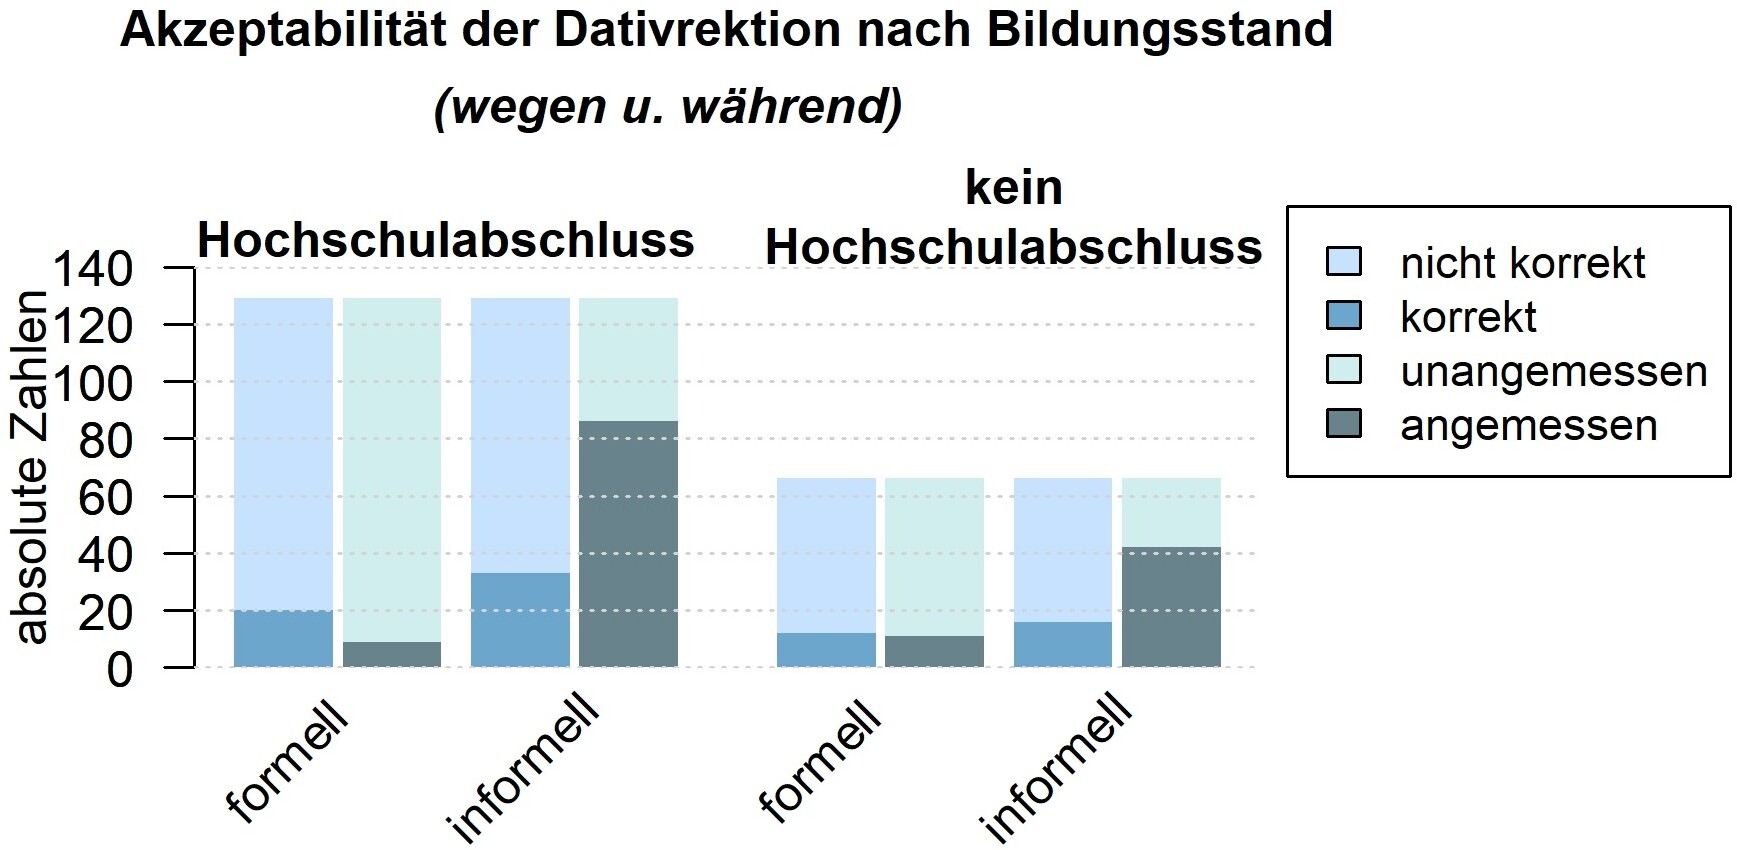
\includegraphics[scale=1]{AkzDativNachBildung.jpg}
%\caption{Akzeptabilität der Dativrektion bei \wegen{} und \waehrend{} nach Bildungsstand}
%\label{pic:AkzDativNachBildung}
%\end{figure}
%\begin{figure}
%\centering
%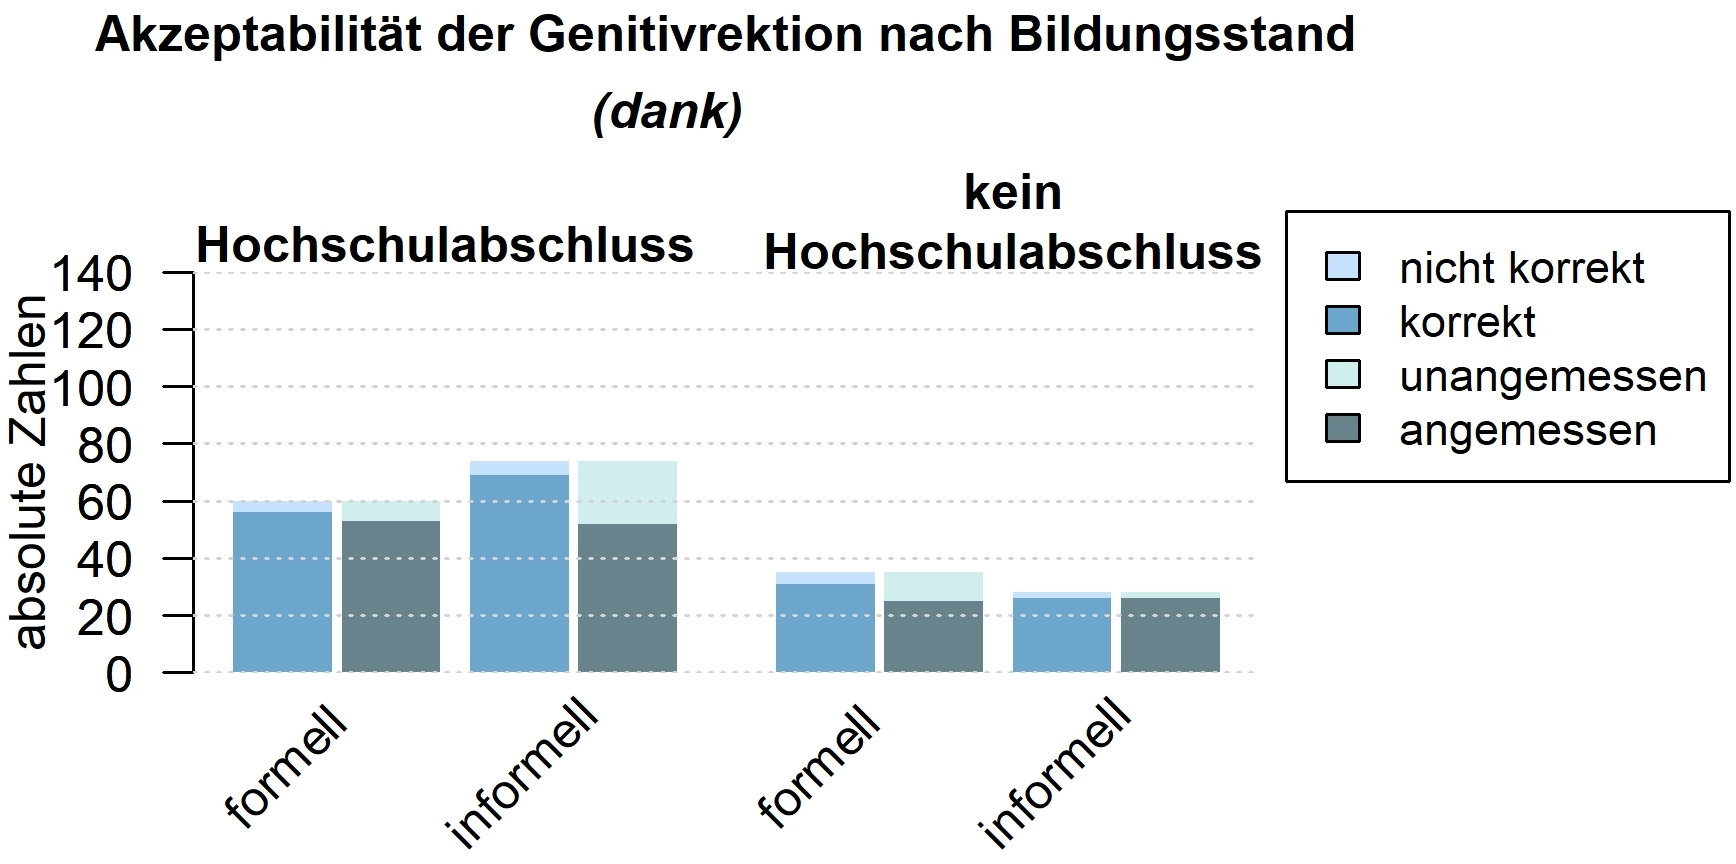
\includegraphics[scale=1]{AkzGenitivNachBildung.jpg}
%\caption{Akzeptabilität der Genitivrektion bei \dank{} nach Bildungsstand}
%\label{pic:AkzGenitivNachBildung}
%\end{figure}
\subsection{Akzeptabilität und Textaffinität des Berufs}
\label{sec:ErgAkzNachBeruf}
Teilweise werden die Varianten im Assoziationsteil nicht nur mit hoher oder niedriger Bildung, sondern auch mit hoher oder niedriger Sprachkompetenz in Verbindung gebracht (\autoref{sec:ErgAssPersonen}). 
Im Folgenden werden daher die Akzeptabilitätswerte von Befragten, die viel mit Sprache zu tun haben, mit denen von Befragten, die wenig mit Sprache zu tun haben, verglichen. 
Zwei Fragen im Fragebogen geben Aufschluss darüber, wie kompetent Personen im Bereich Sprache sind: 
Zum einen die Likertskala zur eigenen Einschätzung der Sprachsicherheit und zum anderen die Frage danach, wie häufig Befragte im Beruf mit längeren Texten zu tun haben (\autoref{sec:RE} und \autoref{sec:ME}). 
Auf der Likertskala zur Einschätzung der Sprachsicherheit erreichen 344 TeilnehmerInnen der Befragung Werte von über drei und sehen sich selbst damit als eher sicher an (\autoref{sec:Sprachsicherheit}). 
Lediglich 53 Befragte erreichen drei oder weniger Punkte auf der Likertskala, stufen ihre eigene Sprachsicherheit also niedrig ein. 
Da diese wenigen Personen im Akzeptabilitätstest auf vier Gruppen verteilt sind, ist die Aussagekraft eines Vergleichs mit der großen Anzahl derer, die sich als sprachlich sicher einstufen, wenig aussagekräftig. 
Zudem misst die Likertskala die Selbsteinschätzung der Befragten, nicht ihre tatsächliche sprachliche Sicherheit. 
Aus diesen Gründen werden für den Vergleich die Angaben zur Sprachaffinität des eigenen Berufs herangezogen (\autoref{sec:Beruf}): 
283 Befragte haben im Beruf täglich mit längeren Texten zu tun und üben damit einen textaffinen Beruf aus. 
114 Befragte haben seltener mit längeren Texten zu tun und üben damit keinen textaffinen Beruf aus. 
Zunächst werden die Ergebnisse zu \wegen{} und \waehrend{} gemeinsam betrachtet, anschließend einzeln die zu \dank{}, \gegenueber{} sowie der Primärpräposition \object{seit}. 

In den beiden Gruppen, die im Akzeptabilitätstest \wegen{} und \waehrend{} bewerten, sind insgesamt 135 Befragte mit textaffinen Berufen und 62 Befragte, deren Berufe nicht textaffin sind (s. \autoref{table:ErgAkzDativNachBeruf}). 
Aus der Gruppe mit textaffinen Berufen beurteilten 69 \wegen{} im formellen und \waehrend{} im informellen Setting und 66 \waehrend{} im formellen und \wegen{} im informellen Setting. 
Von den Befragten ohne textaffine Berufe wurden 32 nach \wegen{} im formellen und \waehrend{} im informellen Setting gefragt und 30 nach \waehrend{} im formellen und \wegen{} im informellen Setting. 
% Please add the following required packages to your document preamble:
% \usepackage{multirow}
% \usepackage[table,xcdraw]{xcolor}
% If you use beamer only pass "xcolor=table" option, i.e. \documentclass[xcolor=table]{beamer}
\begin{table}
\centering
\begin{tabular}{llrrrr}
\multicolumn{6}{l}{\wegen{} oder \waehrend{} + Dativ nach Textaffinität des Berufs}                                                                                                                                                                                                                          \\ \hline
                                                                                &                                      & \multicolumn{2}{c}{\begin{tabular}[c]{@{}c@{}}Beruf\\ textaffin\\ (n=135)\end{tabular}} & \multicolumn{2}{c}{\begin{tabular}[c]{@{}c@{}}Beruf nicht\\ textaffin\\ (n=62)\end{tabular}} \\ \hline
                                                                                & \cellcolor[HTML]{9B9B9B}korrekt      & \cellcolor[HTML]{9B9B9B}17              & \cellcolor[HTML]{9B9B9B}{\footnotesize (12,59 \%)}            & \cellcolor[HTML]{9B9B9B}15                & \cellcolor[HTML]{9B9B9B}{\footnotesize (24,19 \%)}               \\ %\cline{2-6} 
                                                                                & \cellcolor[HTML]{9B9B9B}inkorrekt    & \cellcolor[HTML]{9B9B9B}118             & \cellcolor[HTML]{9B9B9B}{\footnotesize (87,41 \%)}            & \cellcolor[HTML]{9B9B9B}47                & \cellcolor[HTML]{9B9B9B}{\footnotesize (75,81 \%)}               \\ %\cline{2-6} 
                                                                                & \cellcolor[HTML]{EFEFEF}angemessen   & \cellcolor[HTML]{EFEFEF}13              & \cellcolor[HTML]{EFEFEF}{\footnotesize (9,63 \%)}             & \cellcolor[HTML]{EFEFEF}    7              & \cellcolor[HTML]{EFEFEF}{\footnotesize (11,29 \%)}               \\ %\cline{2-6} 
                                                                                & \cellcolor[HTML]{EFEFEF}unangemessen & \cellcolor[HTML]{EFEFEF}122             & \cellcolor[HTML]{EFEFEF}{\footnotesize (90,37 \%)}            & \cellcolor[HTML]{EFEFEF}55                & \cellcolor[HTML]{EFEFEF}{\footnotesize (88,71 \%)}               \\ %\cline{2-6} 
                                                                                & eigene Verwendung ja                 & 7                                       & {\footnotesize (5,19 \%)}                                     & 9                                         & {\footnotesize (14,52 \%)}                                       \\ %\cline{2-6} 
\multirow{-6}{*}{\begin{tabular}[c]{@{}l@{}}formelles\\ Setting\end{tabular}}   & eigene Verwendung nein               & 128                                     & {\footnotesize (94,81 \%)}                                    & 53                                        & {\footnotesize (85,48 \%)}                                       \\ \hline
                                                                                &                                      & \multicolumn{2}{c}{\begin{tabular}[c]{@{}c@{}}Beruf\\ textaffin\\ (n=135)\end{tabular}} & \multicolumn{2}{c}{\begin{tabular}[c]{@{}c@{}}Beruf nicht\\ textaffin\\ (n=62)\end{tabular}} \\ \hline
                                                                                & \cellcolor[HTML]{9B9B9B}korrekt      & \cellcolor[HTML]{9B9B9B}28              & \cellcolor[HTML]{9B9B9B}{\footnotesize (20,74 \%)}            & \cellcolor[HTML]{9B9B9B}22                & \cellcolor[HTML]{9B9B9B}{\footnotesize (35,48 \%)}               \\ %\cline{2-6} 
                                                                                & \cellcolor[HTML]{9B9B9B}inkorrekt    & \cellcolor[HTML]{9B9B9B}107             & \cellcolor[HTML]{9B9B9B}{\footnotesize (79,26 \%)}            & \cellcolor[HTML]{9B9B9B}40                & \cellcolor[HTML]{9B9B9B}{\footnotesize (64,52 \%)}               \\ %\cline{2-6} 
                                                                                & \cellcolor[HTML]{EFEFEF}angemessen   & \cellcolor[HTML]{EFEFEF}89              & \cellcolor[HTML]{EFEFEF}{\footnotesize (65,93 \%)}            & \cellcolor[HTML]{EFEFEF}41                & \cellcolor[HTML]{EFEFEF}{\footnotesize (66,13 \%)}               \\ %\cline{2-6} 
                                                                                & \cellcolor[HTML]{EFEFEF}unangemessen & \cellcolor[HTML]{EFEFEF}46              & \cellcolor[HTML]{EFEFEF}{\footnotesize (34,07 \%)}            & \cellcolor[HTML]{EFEFEF}21                & \cellcolor[HTML]{EFEFEF}{\footnotesize (33,87 \%)}               \\ %\cline{2-6} 
                                                                                & eigene Verwendung ja                 & 61                                      & {\footnotesize (45,19 \%)}                                    & 35                                        & {\footnotesize (56,45 \%)}                                       \\ %\cline{2-6} 
\multirow{-6}{*}{\begin{tabular}[c]{@{}l@{}}informelles\\ Setting\end{tabular}} & eigene Verwendung nein               & 74                                      & {\footnotesize (54,81 \%)}                                    & 27                                        & {\footnotesize (43,55 \%)}                                       \\  \hline
\end{tabular}
\caption{Akzeptabilität der Dativrektion bei \wegen{} und \waehrend{} nach Textaffinität des Berufs}
\label{table:ErgAkzDativNachBeruf}
\end{table}

Befragte aus nicht-textaffinen Berufen beurteilen die Dativrektion bei \wegen{} oder \waehrend{} in beiden Settings häufiger als korrekt, die Angemessenheit schätzen sie jedoch jeweils ganz ähnlich ein wie Befragte aus textaffinen Berufen. 
Während Letztere die Dativrektion bei \wegen{} oder \waehrend{} im formellen Setting nur zu ungefähr 13~\% als korrekt erachten und zu ca. 10~\% als angemessen, empfinden in der Gruppe ohne textaffine Berufe hier rund 24~\% den Dativ als korrekt und ca. 11~\% als angemessen. 
Beide Gruppen bewerten die Varianten im informellen Setting häufiger als korrekt (ca. 21~\% aus textaffinen Berufen und 35,5~\% aus nicht-textaffinen Berufen) und als angemessen (jeweils rund 66~\%). 
Die Diskrepanz zwischen der Beurteilung der Korrektheit und der Angemessenheit ist im formellen Setting also bei Befragten aus nicht-textaffinen Berufen größer, im informellen Setting hingegen bei Befragten aus textaffinen Berufen. 
Die Frage, ob sie die Variante selbst verwenden würden, bejahen von den Befragten ohne textaffine Berufe in beiden Settings etwas mehr als von den Befragten mit textaffinen Berufen. 

Die Genitivrektion bei \dank{} wurde im formellen Setting von 68 Befragten aus textaffinen Berufen und 28 Befragten aus nicht-textaffinen Berufen beurteilt (s. \autoref{table:ErgAkzDankNachBeruf}). 
Im informellen Setting bewerteten die Variante 80 Befragte mit textaffinen Berufen und 24 Befragte ohne textaffine Berufe.
Die Prozentangaben in \autoref{table:ErgAkzDankNachBeruf} für die Gruppe ohne textaffine Berufe sind also mit Vorsicht zu betrachten. 
% Please add the following required packages to your document preamble:
% \usepackage{multirow}
% \usepackage[table,xcdraw]{xcolor}
% If you use beamer only pass "xcolor=table" option, i.e. \documentclass[xcolor=table]{beamer}
\begin{table}
\centering
\begin{tabular}{llrrrr}
\multicolumn{6}{l}{\dank{} + Genitiv nach Textaffinität des Berufs}                                                                                                                                                                                                                                      \\ \hline
                                                                                &                                      & \multicolumn{2}{c}{\begin{tabular}[c]{@{}c@{}}Beruf\\textaffin\\ (n=68)\end{tabular}} & \multicolumn{2}{c}{\begin{tabular}[c]{@{}c@{}}Beruf nicht\\textaffin\\ (n=28)\end{tabular}} \\ \hline
                                                                                & \cellcolor[HTML]{9B9B9B}korrekt      & \cellcolor[HTML]{9B9B9B}63             & \cellcolor[HTML]{9B9B9B}{\footnotesize (92,65 \%)}            & \cellcolor[HTML]{9B9B9B}24                & \cellcolor[HTML]{9B9B9B}{\footnotesize (85,71 \%)}               \\ %\cline{2-6} 
                                                                                & \cellcolor[HTML]{9B9B9B}inkorrekt    & \cellcolor[HTML]{9B9B9B}5              & \cellcolor[HTML]{9B9B9B}{\footnotesize (7,35 \%)}             & \cellcolor[HTML]{9B9B9B}4                 & \cellcolor[HTML]{9B9B9B}{\footnotesize (14,29 \%)}               \\ %\cline{2-6} 
                                                                                & \cellcolor[HTML]{EFEFEF}angemessen   & \cellcolor[HTML]{EFEFEF}57             & \cellcolor[HTML]{EFEFEF}{\footnotesize (83,82 \%)}            & \cellcolor[HTML]{EFEFEF}21                & \cellcolor[HTML]{EFEFEF}{\footnotesize (75 \%)}                  \\ %\cline{2-6} 
                                                                                & \cellcolor[HTML]{EFEFEF}unangemessen & \cellcolor[HTML]{EFEFEF}11             & \cellcolor[HTML]{EFEFEF}{\footnotesize (16,18 \%)}            & \cellcolor[HTML]{EFEFEF}7                 & \cellcolor[HTML]{EFEFEF}{\footnotesize (25 \%)}                  \\ %\cline{2-6} 
                                                                                & eigene Verwendung ja                 & 49                                     & {\footnotesize (72,06 \%)}                                    & 19                                        & {\footnotesize (67,86 \%)}                                       \\ %\cline{2-6} 
\multirow{-6}{*}{\begin{tabular}[c]{@{}l@{}}formelles\\ Setting\end{tabular}}   & eigene Verwendung nein               & 19                                     & {\footnotesize (27,94 \%)}                                    & 9                                         & {\footnotesize (32,14 \%)}                                       \\ \hline
                                                                                &                                      & \multicolumn{2}{c}{\begin{tabular}[c]{@{}c@{}}Beruf\\textaffin\\ (n=80)\end{tabular}} & \multicolumn{2}{c}{\begin{tabular}[c]{@{}c@{}}Beruf nicht\\textaffin\\ (n=24)\end{tabular}} \\ \hline
                                                                                & \cellcolor[HTML]{9B9B9B}korrekt      & \cellcolor[HTML]{9B9B9B}75             & \cellcolor[HTML]{9B9B9B}{\footnotesize (93,75 \%)}            & \cellcolor[HTML]{9B9B9B}22                & \cellcolor[HTML]{9B9B9B}{\footnotesize (91,67 \%)}               \\ %\cline{2-6} 
                                                                                & \cellcolor[HTML]{9B9B9B}inkorrekt    & \cellcolor[HTML]{9B9B9B}5              & \cellcolor[HTML]{9B9B9B}{\footnotesize (6,25 \%)}             & \cellcolor[HTML]{9B9B9B}2                 & \cellcolor[HTML]{9B9B9B}{\footnotesize (8,33 \%)}                \\ %\cline{2-6} 
                                                                                & \cellcolor[HTML]{EFEFEF}angemessen   & \cellcolor[HTML]{EFEFEF}60             & \cellcolor[HTML]{EFEFEF}{\footnotesize (75 \%)}               & \cellcolor[HTML]{EFEFEF}20                & \cellcolor[HTML]{EFEFEF}{\footnotesize (83,33 \%)}               \\ %\cline{2-6} 
                                                                                & \cellcolor[HTML]{EFEFEF}unangemessen & \cellcolor[HTML]{EFEFEF}20             & \cellcolor[HTML]{EFEFEF}{\footnotesize (25 \%)}               & \cellcolor[HTML]{EFEFEF}4                 & \cellcolor[HTML]{EFEFEF}{\footnotesize (16,67 \%)}               \\ %\cline{2-6} 
                                                                                & eigene Verwendung ja                 & 60                                     & {\footnotesize (75 \%)}                                       & 16                                        & {\footnotesize (66,67 \%)}                                       \\ %\cline{2-6} 
\multirow{-6}{*}{\begin{tabular}[c]{@{}l@{}}informelles\\ Setting\end{tabular}} & eigene Verwendung nein               & 20                                     & {\footnotesize (25 \%)}                                       & 8                                         & {\footnotesize (33,33 \%)}                                       \\ \hline 
\end{tabular}
\caption{Akzeptabilität der Genitivrektion bei \dank{} nach Textaffinität des Berufs}
\label{table:ErgAkzDankNachBeruf}
\end{table}
 In beiden Settings zeigen sich zwischen den beiden Gruppen nur geringe Unterschiede in den Angaben zu Korrektheit, Angemessenheit und eigener Verwendung, die sich aufgrund der geringen Zahl Befragter ohne textaffine Berufe kaum interpretieren lassen.

Da die gleichen Gruppen von Befragten, die im Akzeptabilitätstest vom Zufallsmechanismus für \dank{} eingeteilt wurden, \gegenueber{} mit dem Genitiv im jeweils anderen Setting bewerteten, sind auch hier die Stichproben für Befragte ohne textaffine Berufe klein (s. \autoref{table:ErgAkzGegenueberNachBeruf}). 
Im formellen Setting sind die Unterschiede zwischen Befragten mit und ohne textaffine Berufe etwas größer als bei \dank:
Von den 80 Befragten aus textaffinen Berufen bewertet jeweils ungefähr ein Drittel \gegenueber{} plus Genitiv als korrekt und angemessen. 
Unter den 24 Befragten aus nicht-textaffinen Berufen sieht jeweils ungefähr die Hälfte die Variante als korrekt und angemessen an. 
Aufgrund der geringen Stichprobe kann es sich allerdings um zufällige Unterschiede handeln. 
% Please add the following required packages to your document preamble:
% \usepackage{multirow}
% \usepackage[table,xcdraw]{xcolor}
% If you use beamer only pass "xcolor=table" option, i.e. \documentclass[xcolor=table]{beamer}
\begin{table}
\centering
\begin{tabular}{llrrrr}
\multicolumn{6}{l}{\gegenueber{} + Genitiv nach Textaffinität des Berufs}                                                                                                                                                                                                                                \\ \hline
                                                                                &                                      & \multicolumn{2}{c}{\begin{tabular}[c]{@{}c@{}}Beruf\\ textaffin\\ (n=80)\end{tabular}} & \multicolumn{2}{c}{\begin{tabular}[c]{@{}c@{}}Beruf nicht\\ textaffin\\ (n=24)\end{tabular}} \\ \hline
                                                                                & \cellcolor[HTML]{9B9B9B}korrekt      & \cellcolor[HTML]{9B9B9B}27             & \cellcolor[HTML]{9B9B9B}{\footnotesize (33,75 \%)}            & \cellcolor[HTML]{9B9B9B}13                & \cellcolor[HTML]{9B9B9B}{\footnotesize (54,17 \%)}               \\ %\cline{2-6} 
                                                                                & \cellcolor[HTML]{9B9B9B}inkorrekt    & \cellcolor[HTML]{9B9B9B}53             & \cellcolor[HTML]{9B9B9B}{\footnotesize (66,25 \%)}            & \cellcolor[HTML]{9B9B9B}11                & \cellcolor[HTML]{9B9B9B}{\footnotesize (45,83 \%)}               \\ %\cline{2-6} 
                                                                                & \cellcolor[HTML]{EFEFEF}angemessen   & \cellcolor[HTML]{EFEFEF}29             & \cellcolor[HTML]{EFEFEF}{\footnotesize (36,25 \%)}            & \cellcolor[HTML]{EFEFEF}12                & \cellcolor[HTML]{EFEFEF}{\footnotesize (50 \%)}                  \\ %\cline{2-6} 
                                                                                & \cellcolor[HTML]{EFEFEF}unangemessen & \cellcolor[HTML]{EFEFEF}51             & \cellcolor[HTML]{EFEFEF}{\footnotesize (63,75 \%)}            & \cellcolor[HTML]{EFEFEF}12                & \cellcolor[HTML]{EFEFEF}{\footnotesize (50 \%)}                  \\ %\cline{2-6} 
                                                                                & eigene Verwendung ja                 & 22                                     & {\footnotesize (27,5 \%)}                                     & 11                                        & {\footnotesize (45,83 \%)}                                       \\ %\cline{2-6} 
\multirow{-6}{*}{\begin{tabular}[c]{@{}l@{}}formelles\\ Setting\end{tabular}}   & eigene Verwendung nein               & 58                                     & {\footnotesize (72,5 \%)}                                     & 13                                        & {\footnotesize (54,17 \%)}                                       \\ \hline
                                                                                &                                      & \multicolumn{2}{c}{\begin{tabular}[c]{@{}c@{}}Beruf\\ textaffin\\ (n=68)\end{tabular}} & \multicolumn{2}{c}{\begin{tabular}[c]{@{}c@{}}Beruf nicht\\ textaffin\\ (n=28)\end{tabular}} \\ \hline
                                                                                & \cellcolor[HTML]{9B9B9B}korrekt      & \cellcolor[HTML]{9B9B9B}21             & \cellcolor[HTML]{9B9B9B}{\footnotesize (30,88 \%)}            & \cellcolor[HTML]{9B9B9B}10                & \cellcolor[HTML]{9B9B9B}{\footnotesize (35,71 \%)}               \\ %\cline{2-6} 
                                                                                & \cellcolor[HTML]{9B9B9B}inkorrekt    & \cellcolor[HTML]{9B9B9B}47             & \cellcolor[HTML]{9B9B9B}{\footnotesize (69,12 \%)}            & \cellcolor[HTML]{9B9B9B}18                & \cellcolor[HTML]{9B9B9B}{\footnotesize (64,29 \%)}               \\ %\cline{2-6} 
                                                                                & \cellcolor[HTML]{EFEFEF}angemessen   & \cellcolor[HTML]{EFEFEF}26             & \cellcolor[HTML]{EFEFEF}{\footnotesize (38,24 \%)}            & \cellcolor[HTML]{EFEFEF}10                & \cellcolor[HTML]{EFEFEF}{\footnotesize (35,71 \%)}               \\ %\cline{2-6} 
                                                                                & \cellcolor[HTML]{EFEFEF}unangemessen & \cellcolor[HTML]{EFEFEF}42             & \cellcolor[HTML]{EFEFEF}{\footnotesize (61,76 \%)}            & \cellcolor[HTML]{EFEFEF}18                & \cellcolor[HTML]{EFEFEF}{\footnotesize (64,29 \%)}               \\ %\cline{2-6} 
                                                                                & eigene Verwendung ja                 & 17                                     & {\footnotesize (25 \%)}                                       & 4                                         & {\footnotesize (14,29 \%)}                                       \\ %\cline{2-6} 
\multirow{-6}{*}{\begin{tabular}[c]{@{}l@{}}informelles\\ Setting\end{tabular}} & eigene Verwendung nein               & 51                                     & {\footnotesize (75 \%)}                                       & 24                                        & {\footnotesize (85,71 \%)}                                       \\  \hline
\end{tabular}
\caption{Akzeptabilität der Genitivrektion bei \gegenueber{} nach Textaffinität des Berufs}
\label{table:ErgAkzGegenueberNachBeruf}
\end{table}

Die Ergebnisse zur Primärpräposition \object{seit} mit dem Genitiv lassen sich besser vergleichen, da diese Form von allen Befragten im Akzeptabilitätstest bewertet wurde (s. \autoref{table:ErgAkzSeitNachBeruf}). 
Es zeigt sich, dass Befragte aus textaffinen Berufen \object{seit} plus Genitiv durchweg negativer bewerten als Befragte aus nicht-textaffinen Berufen. 
Im formellen Setting beurteilen Erstere die Form zu rund 27~\% als korrekt und zu ca. 28~\% als angemessen. 
Ungefähr 23~\% geben an, die Genitivrektion bei \object{seit} in einem förmlichen Brief an ein Amt selbst zu verwenden. 
Unter den Befragten ohne textaffine Berufe empfinden jeweils rund 45~\% die abgefragte Form im formellen Setting als korrekt und angemessen, ca. 40~\% geben an, sie selbst zu verwenden. 
Unter den Befragten mit textaffinen Berufen beurteilen im informellen Setting nur jeweils etwas weniger \object{seit} plus Genitiv als korrekt und angemessen. 
Befragte aus nicht-textaffinen Berufen hingegen bewerten Korrekhteit und Angemessenheit bei \object{seit} stärker kontextabhängig. 
Zwar ist der Anteil derer, die angeben, die Form sei korrekt und angemessen und würde von ihnen verwendet, unter den Befragten aus nicht-textaffinen Berufen im informellen Setting immer noch größer. 
Die Differenzen zwischen den Gruppen sind hier aber kleiner.
% Please add the following required packages to your document preamble:
% \usepackage{multirow}
% \usepackage[table,xcdraw]{xcolor}
% If you use beamer only pass "xcolor=table" option, i.e. \documentclass[xcolor=table]{beamer}
\begin{table}
\centering
\begin{tabular}{llrrrr}
\multicolumn{6}{l}{\object{seit} + Genitiv nach Textaffinität des Berufs}                                                                                                                                                                                                                                        \\ \hline
                                                                                &                                      & \multicolumn{2}{c}{\begin{tabular}[c]{@{}c@{}}Beruf\\ textaffin\\ (n=283)\end{tabular}} & \multicolumn{2}{c}{\begin{tabular}[c]{@{}c@{}}Beruf nicht\\ textaffin\\ (n=114)\end{tabular}} \\ \hline
                                                                                & \cellcolor[HTML]{9B9B9B}korrekt      & \cellcolor[HTML]{9B9B9B}76              & \cellcolor[HTML]{9B9B9B}{\footnotesize (26,86 \%)}            & \cellcolor[HTML]{9B9B9B}51                & \cellcolor[HTML]{9B9B9B}{\footnotesize (44,74 \%)}                \\ %\cline{2-6} 
                                                                                & \cellcolor[HTML]{9B9B9B}inkorrekt    & \cellcolor[HTML]{9B9B9B}207             & \cellcolor[HTML]{9B9B9B}{\footnotesize (73,14 \%)}            & \cellcolor[HTML]{9B9B9B}63                & \cellcolor[HTML]{9B9B9B}{\footnotesize (55,26 \%)}                \\ %\cline{2-6} 
                                                                                & \cellcolor[HTML]{EFEFEF}angemessen   & \cellcolor[HTML]{EFEFEF}80              & \cellcolor[HTML]{EFEFEF}{\footnotesize (28,27 \%)}            & \cellcolor[HTML]{EFEFEF}51                & \cellcolor[HTML]{EFEFEF}{\footnotesize (44,74 \%)}                \\ %\cline{2-6} 
                                                                                & \cellcolor[HTML]{EFEFEF}unangemessen & \cellcolor[HTML]{EFEFEF}203             & \cellcolor[HTML]{EFEFEF}{\footnotesize (71,73 \%)}            & \cellcolor[HTML]{EFEFEF}63                & \cellcolor[HTML]{EFEFEF}{\footnotesize (55,26 \%)}                \\ %\cline{2-6} 
                                                                                & eigene Verwendung ja                 & 65                                      & {\footnotesize (22,97 \%)}                                    & 45                                        & {\footnotesize (39,47 \%)} \\ %\cline{2-6} 
\multirow{-6}{*}{\begin{tabular}[c]{@{}l@{}}formelles\\ Setting\end{tabular}}   & eigene Verwendung nein               & 218                                     & {\footnotesize (77,03 \%)}                                    & 69                                        & {\footnotesize (60,53 \%)}   \\ \hline
                                                                                &                                      & \multicolumn{2}{c}{\begin{tabular}[c]{@{}c@{}}Beruf\\ textaffin\\ (n=283)\end{tabular}} & \multicolumn{2}{c}{\begin{tabular}[c]{@{}c@{}}Beruf nicht\\ textaffin\\ (n=114)\end{tabular}} \\ \hline
                                                                                & \cellcolor[HTML]{9B9B9B}korrekt      & \cellcolor[HTML]{9B9B9B}50              & \cellcolor[HTML]{9B9B9B}{\footnotesize (17,67 \%)}            & \cellcolor[HTML]{9B9B9B}36                & \cellcolor[HTML]{9B9B9B}{\footnotesize (31,58 \%)}                \\ %\cline{2-6} 
                                                                                & \cellcolor[HTML]{9B9B9B}inkorrekt    & \cellcolor[HTML]{9B9B9B}233             & \cellcolor[HTML]{9B9B9B}{\footnotesize (82,33 \%)}            & \cellcolor[HTML]{9B9B9B}78                & \cellcolor[HTML]{9B9B9B}{\footnotesize (68,42 \%)}                \\ %\cline{2-6} 
                                                                                & \cellcolor[HTML]{EFEFEF}angemessen   & \cellcolor[HTML]{EFEFEF}60              & \cellcolor[HTML]{EFEFEF}{\footnotesize (21,2 \%)}             & \cellcolor[HTML]{EFEFEF}34                & \cellcolor[HTML]{EFEFEF}{\footnotesize (29,82 \%)}                \\ %\cline{2-6} 
                                                                                & \cellcolor[HTML]{EFEFEF}unangemessen & \cellcolor[HTML]{EFEFEF}223             & \cellcolor[HTML]{EFEFEF}{\footnotesize (78,8 \%)}             & \cellcolor[HTML]{EFEFEF}80                & \cellcolor[HTML]{EFEFEF}{\footnotesize (70,18 \%)}                \\ %\cline{2-6} 
                                                                                & eigene Verwendung ja                 & 27                                      & {\footnotesize (9,54 \%)}                                     & 24                                        & {\footnotesize (21,05 \%)}                                        \\ %\cline{2-6} 
\multirow{-6}{*}{\begin{tabular}[c]{@{}l@{}}informelles\\ Setting\end{tabular}} & eigene Verwendung nein               & 256                                     & {\footnotesize (90,46 \%)}                                    & 90                                        & {\footnotesize (78,95 \%)}                                        \\ \hline
\end{tabular}
\caption{Akzeptabilität der Genitivrektion bei \object{seit} nach Textaffinität des Berufs}
\label{table:ErgAkzSeitNachBeruf}
\end{table}

Der Vergleich der Akzeptabilitätsangaben von Befragten, die im Beruf häufig oder täglich mit längeren Texten zu tun haben, und Befragten, die im Beruf seltener mit längeren Texten zu tun haben, ergibt zusammengefassst folgende Ergebnisse:
Die Dativrektion bei \wegen{} und \waehrend{} wird von Befragten aus textaffinen Berufen in beiden Settings etwas seltener als korrekt bewertet. 
Sie geben auch seltener an, diese Formen selbst zu verwenden. 
Die Angemessenheit wird jedoch in beiden Gruppen ähnlich beurteilt. 
Bei \dank{} und \gegenueber{} mit der Genitivrektion zeigen sich nur geringe Unterschiede, die sich aufgrund der kleinen Stichproben nicht deuten lassen. 
Die Primärpräposition \object{seit} mit der Genitivrektion wird von Befragten aus textaffinen Berufen in beiden Settings seltener als korrekt und angemessen bewertet. 
Die Frage nach der eigenen Verwendung bejahen hier unter den Befragten aus textaffinen Berufen ebenfalls weniger. 
\subsection{Akzeptabilität und Variationstoleranz}
\label{sec:ErgAkzNachVT}
% Akzeptabilität nach Variationstoleranz
Wie in \autoref{sec:Variationstoleranz} dargestellt, unterscheiden sich die Befragten in ihrer Toleranz gegenüber sprachlicher Variation. 
Sie lassen sich in eher variationstolerante und eher wenig variationstolerante Personen unterteilen. 
Hierfür werden ihre Antworten auf der Likertskala zur Variationstoleranz am Beginn des Fragebogens herangezogen: 
Personen, die auf der Likertskala zur Variationstoleranz Werte zwischen null und drei erreichen, bilden die wenig variationstolerante Gruppe (abgekürzt als Vt--), während Personen, die Werte von über drei erreichen, als variationstolerant gelten können (abgekürzt als Vt+). 
Ob Befragte, die Variation gegenüber generell offener sind, sich im Akzeptabilitätstest anders verhalten als Befragte, die Variation ablehnen, ist Thema dieses Abschnitts. 
Wieder werden erst die summierten Akzeptabilitätswerte zu \wegen{} und \waehrend{}, dann einzeln die zu \dank{}, \gegenueber{} und der Primärpräposition \object{seit} betrachtet. 

Von den Befragten, die im Akzeptabilitätstest in einer der beiden Gruppen mit den ursprünglichen Genitivpräpositionen \wegen{} und \waehrend{} waren, können 108 aufgrund ihrer Antworten auf der Likertskala als variationstolerant (Vt+) eingestuft werden (s. \autoref{table:ErgAkzDativNachVT}).
Davon bewertete genau die Hälfte (54) \wegen{} im formellen und \waehrend{} im informellen Kontext, bei der anderen Hälfte wurden die Präpositionen im jeweils anderen Kontext abgefragt. 
89 Befragte, die im Akzeptabilitätstest \wegen{} oder \waehrend{} beurteilten, können als weniger variationstolerant (Vt--) klassifiziert werden.
47 von ihnen wurden im formellen Setting nach der Akzeptabilität von \wegen{} plus Dativ gefragt und im informellen Setting nach der Akzeptabilität von \waehrend{} plus Dativ. 
Bei 42 Befragten der Gruppe Vt-- war die Verteilung der Präpositionen auf die Settings umgekehrt. 
% Please add the following required packages to your document preamble:
% \usepackage{multirow}
% \usepackage[table,xcdraw]{xcolor}
% If you use beamer only pass "xcolor=table" option, i.e. \documentclass[xcolor=table]{beamer}
\begin{table}
\centering
\begin{tabular}{llrrrr}
\multicolumn{6}{l}{\wegen{} oder \waehrend{} + Dativ nach Variationstoleranz}                                                                                                                                                                                               \\ \hline
                                                                                &                                      & \multicolumn{2}{c}{\begin{tabular}[c]{@{}c@{}}Vt+\\ (n=108)\end{tabular}} & \multicolumn{2}{c}{\begin{tabular}[c]{@{}c@{}}Vt--\\ (n=89)\end{tabular}} \\ \hline
                                                                                & \cellcolor[HTML]{9B9B9B}korrekt      & \cellcolor[HTML]{9B9B9B}19      & \cellcolor[HTML]{9B9B9B}{\footnotesize (17,59 \%)}       & \cellcolor[HTML]{9B9B9B}13      & \cellcolor[HTML]{9B9B9B}{\footnotesize (14,61 \%)}      \\ %\cline{2-6} 
                                                                                & \cellcolor[HTML]{9B9B9B}inkorrekt    & \cellcolor[HTML]{9B9B9B}89      & \cellcolor[HTML]{9B9B9B}{\footnotesize (82,41 \%)}      & \cellcolor[HTML]{9B9B9B}76      & \cellcolor[HTML]{9B9B9B}{\footnotesize (85,39 \%)}      \\ %\cline{2-6} 
                                                                                & \cellcolor[HTML]{EFEFEF}angemessen   & \cellcolor[HTML]{EFEFEF}12      & \cellcolor[HTML]{EFEFEF}{\footnotesize (11,11 \%)}      & \cellcolor[HTML]{EFEFEF}8       & \cellcolor[HTML]{EFEFEF}{\footnotesize (8,99 \%)}       \\ %\cline{2-6} 
                                                                                & \cellcolor[HTML]{EFEFEF}unangemessen & \cellcolor[HTML]{EFEFEF}96      & \cellcolor[HTML]{EFEFEF}{\footnotesize (88,89 \%)}      & \cellcolor[HTML]{EFEFEF}81      & \cellcolor[HTML]{EFEFEF}{\footnotesize (91,01 \%)}      \\ %\cline{2-6} 
                                                                                & eigene Verwendung ja                 & 12                              & {\footnotesize (11,11 \%)}                              & 4                               & {\footnotesize (4,49 \%)}                               \\ %\cline{2-6} 
\multirow{-6}{*}{\begin{tabular}[c]{@{}l@{}}formelles\\ Setting\end{tabular}}   & eigene Verwendung nein               & 96                              & {\footnotesize (88,89 \%)}                              & 85                              & {\footnotesize (95,51 \%)}                              \\ \hline
                                                                                &                                      & \multicolumn{2}{c}{\begin{tabular}[c]{@{}c@{}}Vt+\\ (n=108)\end{tabular}} & \multicolumn{2}{c}{\begin{tabular}[c]{@{}c@{}}Vt--\\ (n=89)\end{tabular}} \\ \hline
                                                                                & \cellcolor[HTML]{9B9B9B}korrekt      & \cellcolor[HTML]{9B9B9B}36      & \cellcolor[HTML]{9B9B9B}{\footnotesize (33,33 \%)}      & \cellcolor[HTML]{9B9B9B}14      & \cellcolor[HTML]{9B9B9B}{\footnotesize (15,73 \%)}      \\ %\cline{2-6} 
                                                                                & \cellcolor[HTML]{9B9B9B}inkorrekt    & \cellcolor[HTML]{9B9B9B}72      & \cellcolor[HTML]{9B9B9B}{\footnotesize (66,67 \%)}      & \cellcolor[HTML]{9B9B9B}75      & \cellcolor[HTML]{9B9B9B}{\footnotesize (84,27 \%)}      \\ %\cline{2-6} 
                                                                                & \cellcolor[HTML]{EFEFEF}angemessen   & \cellcolor[HTML]{EFEFEF}79      & \cellcolor[HTML]{EFEFEF}{\footnotesize (73,15 \%)}      & \cellcolor[HTML]{EFEFEF}51      & \cellcolor[HTML]{EFEFEF}{\footnotesize (57,3 \%)}       \\ %\cline{2-6} 
                                                                                & \cellcolor[HTML]{EFEFEF}unangemessen & \cellcolor[HTML]{EFEFEF}29      & \cellcolor[HTML]{EFEFEF}{\footnotesize (26,85 \%)}      & \cellcolor[HTML]{EFEFEF}38      & \cellcolor[HTML]{EFEFEF}{\footnotesize (42,7 \%)}       \\ %\cline{2-6} 
                                                                                & eigene Verwendung ja                 & 64                              & {\footnotesize (59,26 \%)}                              & 32                              & {\footnotesize (35,96 \%)}                              \\ %\cline{2-6} 
\multirow{-6}{*}{\begin{tabular}[c]{@{}l@{}}informelles\\ Setting\end{tabular}} & eigene Verwendung nein               & 44                              & {\footnotesize (40,74 \%)}                              & 57                              & {\footnotesize (64,04 \%)}                              \\ \hline
\end{tabular}
\caption{Akzeptabilität der Dativrektion bei \wegen{} und \waehrend{} nach Variationstoleranz}
\label{table:ErgAkzDativNachVT}
\end{table}

Ein interessantes Ergebnis des Vergleichs der Gruppe Vt+ mit der Gruppe Vt-- ist, dass sich die Gruppen offenbar in ihrer Beurteilung der Korrektheit der Dativrektion unterscheiden: 
Diese wird von den Befragten, die Variation eher ablehnen, unabhängig vom Kontext bewertet.
In einem Brief an ein Amt empfinden 76 von 89 wenig variationstoleranten Befragten die Dativrektion als inkorrekt, in einem Gespräch mit einem Freund 75. 
Befragte der Gruppe Vt+ hingegen ordnen die Dativrektion im informellen Setting deutlich häufiger (36-mal) als korrekt ein als im formellen Setting (19-mal). 
Die Angemessenheit der Varianten wird von allen Befragten unabhängig von ihrer Variationstoleranz in Abhängigkeit vom Kontext beurteilt.
Der Anteil derer, die den Dativ im informellen Kontext als angemessen ansehen, ist unter den variationstoleranten Befragten jedoch höher als unter den nicht variationstoleranten (79 von 108 im Vergleich zu 51 von 89). 

Im informellen Setting zeigen sich zudem große Unterschiede bei den Angaben zur eigenen Verwendung. 
Eine Mehrheit der variationstoleranten Befragten würde die Dativrektion bei \wegen{} oder \waehrend{} verwenden (64 von 108), von den nicht variationstoleranten Befragten gibt dies jedoch nur ca. ein Drittel an (32 von 89). 

Die beiden Gruppen, die aufgrund des Zufallsmechanismus im Akzeptabilitätstest die Genitivrektion bei ursprünglichen Dativpräpositionen beurteilten, teilen sich wie folgt auf: 
59 Befragte der Gruppe Vt+ und 37 Befragte der Gruppe Vt-- bewerteten \dank{} im formellen und \gegenueber{} im informellen Setting (s. \autoref{table:ErgAkzDankNachVT} und \autoref{table:ErgAkzGegenueberNachVT}). 
61 Befragte der Gruppe Vt+ und 43 Befragte der Gruppe Vt-- beurteilten umgekehrt \gegenueber{} im formellen und \dank{} im informellen Setting. 

Bei \dank{} plus Genitiv zeigen sich wenig nennenswerte Unterschiede zwischen den Gruppen.
Die Variante wird mehrheitlich akzeptiert. 
Im formellen Kontext wird die Genitivrektion bei \dank{} von Befragten der Gruppe Vt-- allerdings eher abgelehnt als von Befragten der Gruppe Vt+: 
Ungefähr ein Drittel der Befragten mit Vt-- empfindet \dank{} plus Genitiv in einem Brief an ein Amt als unangemessen. 
Unter den Befragten mit Vt+ ist der Anteil kleiner (sieben von 59). 
% Please add the following required packages to your document preamble:
% \usepackage{multirow}
% \usepackage[table,xcdraw]{xcolor}
% If you use beamer only pass "xcolor=table" option, i.e. \documentclass[xcolor=table]{beamer}
\begin{table}
\centering
\begin{tabular}{llrrrr}
\multicolumn{6}{l}{\dank{} + Genitiv nach Variationstoleranz}                                                                                                                                                                                                           \\ \hline
                                                                                &                                      & \multicolumn{2}{c}{\begin{tabular}[c]{@{}c@{}}Vt+\\ (n=59)\end{tabular}} & \multicolumn{2}{c}{\begin{tabular}[c]{@{}c@{}}Vt--\\ (n=37)\end{tabular}} \\ \hline
                                                                                & \cellcolor[HTML]{9B9B9B}korrekt      & \cellcolor[HTML]{9B9B9B}55      & \cellcolor[HTML]{9B9B9B}{\footnotesize (93,22 \%)}     & \cellcolor[HTML]{9B9B9B}32      & \cellcolor[HTML]{9B9B9B}{\footnotesize (86,49 \%)}      \\ %\cline{2-6} 
                                                                                & \cellcolor[HTML]{9B9B9B}inkorrekt    & \cellcolor[HTML]{9B9B9B}4       & \cellcolor[HTML]{9B9B9B}{\footnotesize (6,78 \%)}      & \cellcolor[HTML]{9B9B9B}5       & \cellcolor[HTML]{9B9B9B}{\footnotesize (13,51 \%)}      \\ %\cline{2-6} 
                                                                                & \cellcolor[HTML]{EFEFEF}angemessen   & \cellcolor[HTML]{EFEFEF}52      & \cellcolor[HTML]{EFEFEF}{\footnotesize (88,14 \%)}     & \cellcolor[HTML]{EFEFEF}26      & \cellcolor[HTML]{EFEFEF}{\footnotesize (70,27 \%)}      \\ %\cline{2-6} 
                                                                                & \cellcolor[HTML]{EFEFEF}unangemessen & \cellcolor[HTML]{EFEFEF}7       & \cellcolor[HTML]{EFEFEF}{\footnotesize (11,86 \%})     & \cellcolor[HTML]{EFEFEF}11      & \cellcolor[HTML]{EFEFEF}{\footnotesize (29,73 \%)}      \\ %\cline{2-6} 
                                                                                & eigene Verwendung ja                 & 47                              & {\footnotesize (79,66 \%)}                             & 21                              & {\footnotesize (56,76 \%)}                              \\ \cline{2-6} 
\multirow{-6}{*}{\begin{tabular}[c]{@{}l@{}}formelles\\ Setting\end{tabular}}   & eigene Verwendung nein               & 12                              & {\footnotesize (20,34 \%)}                             & 16                              & {\footnotesize (43,24 \%)}                              \\ \hline
                                                                                &                                      & \multicolumn{2}{c}{\begin{tabular}[c]{@{}c@{}}Vt+\\ (n=61)\end{tabular}} & \multicolumn{2}{c}{\begin{tabular}[c]{@{}c@{}}Vt--\\ (n=43)\end{tabular}} \\ \hline
                                                                                & \cellcolor[HTML]{9B9B9B}korrekt      & \cellcolor[HTML]{9B9B9B}57      & \cellcolor[HTML]{9B9B9B}{\footnotesize (93,44 \%)}     & \cellcolor[HTML]{9B9B9B}40      & \cellcolor[HTML]{9B9B9B}{\footnotesize (93,02 \%)}      \\ %\cline{2-6} 
                                                                                & \cellcolor[HTML]{9B9B9B}inkorrekt    & \cellcolor[HTML]{9B9B9B}4       & \cellcolor[HTML]{9B9B9B}{\footnotesize (6,56 \%)}      & \cellcolor[HTML]{9B9B9B}3       & \cellcolor[HTML]{9B9B9B}{\footnotesize (6,98 \%)}       \\ %\cline{2-6} 
                                                                                & \cellcolor[HTML]{EFEFEF}angemessen   & \cellcolor[HTML]{EFEFEF}46      & \cellcolor[HTML]{EFEFEF}{\footnotesize (75,41 \%)}     & \cellcolor[HTML]{EFEFEF}34      & \cellcolor[HTML]{EFEFEF}{\footnotesize (79,07 \%)}      \\ %\cline{2-6} 
                                                                                & \cellcolor[HTML]{EFEFEF}unangemessen & \cellcolor[HTML]{EFEFEF}15      & \cellcolor[HTML]{EFEFEF}{\footnotesize (24,59 \%)}     & \cellcolor[HTML]{EFEFEF}9       & \cellcolor[HTML]{EFEFEF}{\footnotesize (20,93 \%)}      \\ %\cline{2-6} 
                                                                                & eigene Verwendung ja                 & 44                              & {\footnotesize (72,13 \%)}                             & 32                              & {\footnotesize (74,42 \%)}                              \\ %\cline{2-6} 
\multirow{-6}{*}{\begin{tabular}[c]{@{}l@{}}informelles\\ Setting\end{tabular}} & eigene Verwendung nein               & 17                              & {\footnotesize (27,87 \%)}                             & 11                              & {\footnotesize (25,58 \%)}                              \\ \hline
\end{tabular}
\caption{Akzeptabilität der Genitivrektion bei \dank{} nach Variationstoleranz}
\label{table:ErgAkzDankNachVT}
\end{table}

\object{Gegenüber} mit dem Genitiv wird von beiden Gruppen gleichermaßen mehrheitlich abgelehnt. 
Im formellen Setting beurteilen Befragte der Gruppe Vt-- die Variante etwas häufiger als korrekt und angemessen. 
Im informellen Setting zeigt sich folgender Unterschied: 
Aus der variationstoleranteren Gruppe finden \gegenueber{} plus Genitiv  etwas mehr Befragte in einem Gespräch mit einem Freund angemessen als korrekt. 
Dies ist in der Gruppe der Befragten mit geringerer Toleranz für Variation nicht der Fall. 
Aufgrund der kleinen Stichprobe kann es sich aber um eine zufällige Verteilung handeln. 
% Please add the following required packages to your document preamble:
% \usepackage{multirow}
% \usepackage[table,xcdraw]{xcolor}
% If you use beamer only pass "xcolor=table" option, i.e. \documentclass[xcolor=table]{beamer}
\begin{table}
\centering
\begin{tabular}{llrrrr}
\multicolumn{6}{l}{\gegenueber{} + Genitiv nach Variationstoleranz}                                                                                                                                                                                                     \\ \hline
                                                                                &                                      & \multicolumn{2}{c}{\begin{tabular}[c]{@{}c@{}}Vt+\\ (n=61)\end{tabular}} & \multicolumn{2}{c}{\begin{tabular}[c]{@{}c@{}}Vt--\\ (n=43)\end{tabular}} \\ \hline
                                                                                & \cellcolor[HTML]{9B9B9B}korrekt      & \cellcolor[HTML]{9B9B9B}21      & \cellcolor[HTML]{9B9B9B}{\footnotesize (34,43 \%)}     & \cellcolor[HTML]{9B9B9B}19      & \cellcolor[HTML]{9B9B9B}{\footnotesize (44,19 \%)}      \\ %\cline{2-6} 
                                                                                & \cellcolor[HTML]{9B9B9B}inkorrekt    & \cellcolor[HTML]{9B9B9B}40      & \cellcolor[HTML]{9B9B9B}{\footnotesize (65,57 \%)}     & \cellcolor[HTML]{9B9B9B}24      & \cellcolor[HTML]{9B9B9B}{\footnotesize (55,81 \%)}      \\ %\cline{2-6} 
                                                                                & \cellcolor[HTML]{EFEFEF}angemessen   & \cellcolor[HTML]{EFEFEF}21      & \cellcolor[HTML]{EFEFEF}{\footnotesize (34,43 \%)}     & \cellcolor[HTML]{EFEFEF}20      & \cellcolor[HTML]{EFEFEF}{\footnotesize (46,51 \%)}      \\ %\cline{2-6} 
                                                                                & \cellcolor[HTML]{EFEFEF}unangemessen & \cellcolor[HTML]{EFEFEF}40      & \cellcolor[HTML]{EFEFEF}{\footnotesize (65,57 \%)}     & \cellcolor[HTML]{EFEFEF}23      & \cellcolor[HTML]{EFEFEF}{\footnotesize (53,49 \%)}      \\ %\cline{2-6} 
                                                                                & eigene Verwendung ja                 & 18                              & {\footnotesize (29,51 \%)}                             & 15                              & {\footnotesize (34,88 \%)}                              \\ %\cline{2-6} 
\multirow{-6}{*}{\begin{tabular}[c]{@{}l@{}}formelles\\ Setting\end{tabular}}   & eigene Verwendung nein               & 43                              & {\footnotesize (70,49 \%)}                             & 28                              & {\footnotesize (65,12 \%)}                              \\ \hline
                                                                                &                                      & \multicolumn{2}{c}{\begin{tabular}[c]{@{}c@{}}Vt+\\ (n=59)\end{tabular}} & \multicolumn{2}{c}{\begin{tabular}[c]{@{}c@{}}Vt--\\ (n=37)\end{tabular}} \\ \hline
                                                                                & \cellcolor[HTML]{9B9B9B}korrekt      & \cellcolor[HTML]{9B9B9B}16      & \cellcolor[HTML]{9B9B9B}{\footnotesize (27,12 \%)}     & \cellcolor[HTML]{9B9B9B}15      & \cellcolor[HTML]{9B9B9B}{\footnotesize (40,54 \%)}      \\ %\cline{2-6} 
                                                                                & \cellcolor[HTML]{9B9B9B}inkorrekt    & \cellcolor[HTML]{9B9B9B}43      & \cellcolor[HTML]{9B9B9B}{\footnotesize (72,88 \%)}     & \cellcolor[HTML]{9B9B9B}22      & \cellcolor[HTML]{9B9B9B}{\footnotesize (59,46 \%)}      \\ %\cline{2-6} 
                                                                                & \cellcolor[HTML]{EFEFEF}angemessen   & \cellcolor[HTML]{EFEFEF}21      & \cellcolor[HTML]{EFEFEF}{\footnotesize (35,59 \%)}     & \cellcolor[HTML]{EFEFEF}15      & \cellcolor[HTML]{EFEFEF}{\footnotesize (40,54 \%)}      \\ %\cline{2-6} 
                                                                                & \cellcolor[HTML]{EFEFEF}unangemessen & \cellcolor[HTML]{EFEFEF}38      & \cellcolor[HTML]{EFEFEF}{\footnotesize (64,41 \%)}     & \cellcolor[HTML]{EFEFEF}22      & \cellcolor[HTML]{EFEFEF}{\footnotesize (59,46 \%)}      \\ %\cline{2-6} 
                                                                                & eigene Verwendung ja                 & 11                              & {\footnotesize (18,64 \%)}                             & 10                              & {\footnotesize (27,03 \%)}                              \\ %\cline{2-6} 
\multirow{-6}{*}{\begin{tabular}[c]{@{}l@{}}informelles\\ Setting\end{tabular}} & eigene Verwendung nein               & 48                              & {\footnotesize (81,36 \%)}                             & 27                              & {\footnotesize (72,97 \%)}                              \\ \hline
\end{tabular}
\caption{Akzeptabilität der Genitivrektion bei \gegenueber{} nach Variationstoleranz}
\label{table:ErgAkzGegenueberNachVT}
\end{table}
%\begin{figure}
%\centering
%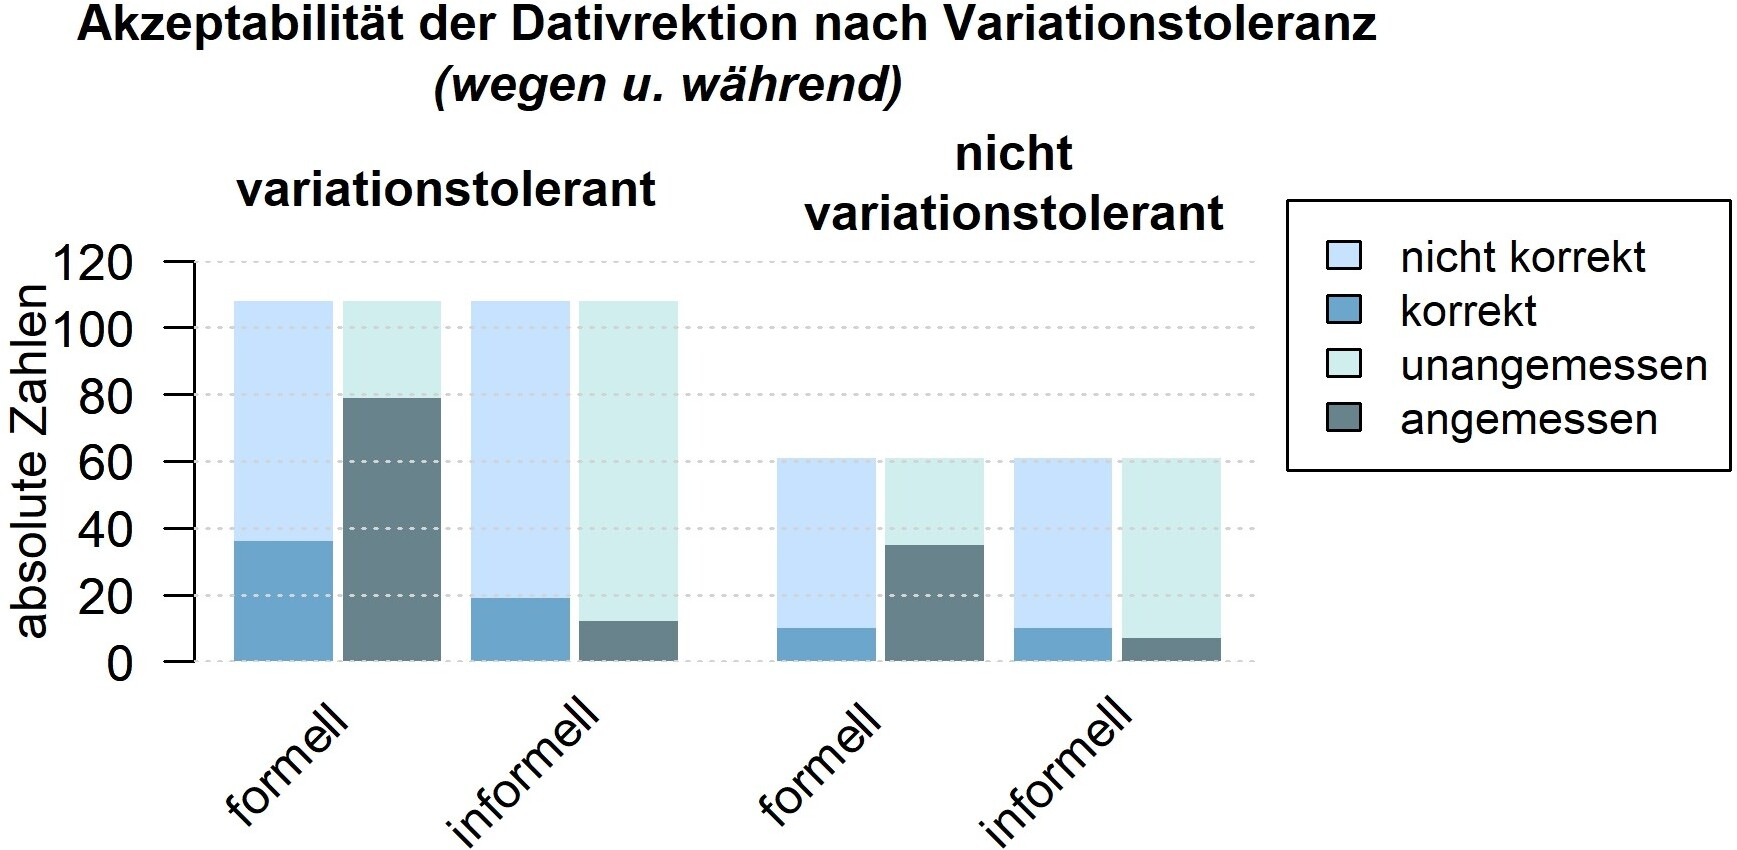
\includegraphics[scale=1]{AkzDativNachVT}
%\caption{Akzeptabilität der Dativrektion bei \wegen{} und \waehrend{} nach Variationstoleranz}
%\label{pic:AkzDativNachVT}
%\end{figure}
%\begin{figure}
%\centering
%\includegraphics[scale=1]{AkzGenitivNAchVT}
%\caption{Akzeptabilität der Genitivrektion bei \dank{} nach Variationstoleranz}
%\label{pic:AkzGenitivNachVT}
%\end{figure}

Bei der Genitivrektion mit der Primärpräposition \object{seit}, die im Akzeptabilitätstest von allen Befragten bewertet wurde, zeigen sich keinerlei Unterschiede zwischen den Gruppen Vt+ und Vt-- (s. \autoref{table:ErgAkzSeitNachVT}). 
% Please add the following required packages to your document preamble:
% \usepackage{multirow}
% \usepackage[table,xcdraw]{xcolor}
% If you use beamer only pass "xcolor=table" option, i.e. \documentclass[xcolor=table]{beamer}
\begin{table}
\centering
\begin{tabular}{llrrrr}
\multicolumn{6}{l}{\object{seit} + Genitiv nach Variationstoleranz}                                                                                                                                                                                                             \\ \hline
                                                                                &                                      & \multicolumn{2}{c}{\begin{tabular}[c]{@{}c@{}}Vt+\\ (n=228)\end{tabular}} & \multicolumn{2}{c}{\begin{tabular}[c]{@{}c@{}}Vt--\\ (n=169)\end{tabular}} \\ \hline
                                                                                & \cellcolor[HTML]{9B9B9B}korrekt      & \cellcolor[HTML]{9B9B9B}72       & \cellcolor[HTML]{9B9B9B}{\footnotesize (31,58 \%)}     & \cellcolor[HTML]{9B9B9B}55       & \cellcolor[HTML]{9B9B9B}{\footnotesize (32,54 \%)}      \\ %\cline{2-6} 
                                                                                & \cellcolor[HTML]{9B9B9B}inkorrekt    & \cellcolor[HTML]{9B9B9B}156      & \cellcolor[HTML]{9B9B9B}{\footnotesize (68,42 \%)}     & \cellcolor[HTML]{9B9B9B}114      & \cellcolor[HTML]{9B9B9B}{\footnotesize (67,46 \%)}      \\ %\cline{2-6} 
                                                                                & \cellcolor[HTML]{EFEFEF}angemessen   & \cellcolor[HTML]{EFEFEF}73       & \cellcolor[HTML]{EFEFEF}{\footnotesize (32,02 \%)}     & \cellcolor[HTML]{EFEFEF}58       & \cellcolor[HTML]{EFEFEF}{\footnotesize (34,32 \%)}      \\ %\cline{2-6} 
                                                                                & \cellcolor[HTML]{EFEFEF}unangemessen & \cellcolor[HTML]{EFEFEF}155      & \cellcolor[HTML]{EFEFEF}{\footnotesize (67,98 \%)}     & \cellcolor[HTML]{EFEFEF}111      & \cellcolor[HTML]{EFEFEF}{\footnotesize (65,68 \%)}      \\ %\cline{2-6} 
                                                                                & eigene Verwendung ja                 & 62                               & {\footnotesize (27,19 \%)}                             & 48                               & {\footnotesize (28,4 \%)}                               \\ %\cline{2-6} 
\multirow{-6}{*}{\begin{tabular}[c]{@{}l@{}}formelles\\ Setting\end{tabular}}   & eigene Verwendung nein               & 166                              & {\footnotesize (72,81 \%)}                             & 121                              & {\footnotesize (71,6 \%)}                               \\ \hline
                                                                                &                                      & \multicolumn{2}{c}{\begin{tabular}[c]{@{}c@{}}Vt+\\ (n=228)\end{tabular}} & \multicolumn{2}{c}{\begin{tabular}[c]{@{}c@{}}Vt--\\ (n=169)\end{tabular}} \\ \hline
                                                                                & \cellcolor[HTML]{9B9B9B}korrekt      & \cellcolor[HTML]{9B9B9B}49       & \cellcolor[HTML]{9B9B9B}{\footnotesize (21,49 \%)}     & \cellcolor[HTML]{9B9B9B}37       & \cellcolor[HTML]{9B9B9B}{\footnotesize (21,89 \%)}      \\ %\cline{2-6} 
                                                                                & \cellcolor[HTML]{9B9B9B}inkorrekt    & \cellcolor[HTML]{9B9B9B}179      & \cellcolor[HTML]{9B9B9B}{\footnotesize (78,51 \%)}     & \cellcolor[HTML]{9B9B9B}132      & \cellcolor[HTML]{9B9B9B}{\footnotesize (78,11 \%)}      \\ %\cline{2-6} 
                                                                                & \cellcolor[HTML]{EFEFEF}angemessen   & \cellcolor[HTML]{EFEFEF}50       & \cellcolor[HTML]{EFEFEF}{\footnotesize (21,93 \%)}     & \cellcolor[HTML]{EFEFEF}44       & \cellcolor[HTML]{EFEFEF}{\footnotesize (26,04 \%)}      \\ %\cline{2-6} 
                                                                                & \cellcolor[HTML]{EFEFEF}unangemessen & \cellcolor[HTML]{EFEFEF}178      & \cellcolor[HTML]{EFEFEF}{\footnotesize (78,07 \%)}     & \cellcolor[HTML]{EFEFEF}125      & \cellcolor[HTML]{EFEFEF}{\footnotesize (73,96 \%)}      \\ %\cline{2-6} 
                                                                                & eigene Verwendung ja                 & 28                               & {\footnotesize (12,28 \%)}                             & 23                               & {\footnotesize (13,61 \%)}                              \\ %\cline{2-6} 
\multirow{-6}{*}{\begin{tabular}[c]{@{}l@{}}informelles\\ Setting\end{tabular}} & eigene Verwendung nein               & 200                              & {\footnotesize (87,72 \%)}                             & 146                              & {\footnotesize (86,39 \%)}                              \\ \hline
\end{tabular}
\caption{Akzeptabilität der Genitivrektion bei \object{seit} nach Variationstoleranz}
\label{table:ErgAkzSeitNachVT}
\end{table}

Insgesamt zeigt der Vergleich der Akzeptabilitätswerte anhand der Variationstoleranz der Befragten, dass die Dativrektion bei \wegen{} und \waehrend{} unter Befragten mit höherer Variationstoleranz im informellen Setting akzeptierter ist als unter Befragten mit geringerer Variationstoleranz.  
Befragte der Gruppe Vt+ bewerten die Varianten hier anteilig häufiger als korrekt und angemessen und würden sie eher selbst verwenden. 
Zudem zeigt sich, dass die Gruppe Vt+ bei der Bewertung der Korrektheit von \wegen{} oder \waehrend{} plus Dativ kontextsensitiver ist: 
Im formellen Setting beurteilen deutlich weniger die Formen als korrekt als im informellen Setting. 
\object{Dank} plus Genitiv scheinen Befragte der Gruppe Vt+ im formellen Setting hingegen eher angemessen zu finden als Befragte der Gruppe Vt--. 
Umgekehrt wertet die Gruppe Vt-- den Genitiv bei \gegenueber{} im formellen Setting eher als angemessen als die Gruppe Vt+. 
Die Primärpräposition \object{seit} mit dem Genitiv wird in beiden Gruppen gleich beurteilt. 
\subsection{\textit{Conditional Inference Trees} und \textit{Random Forests} für den Akzeptabilitätstest}
\label{sec:ErgAkzCTrees}
Bisher wurden folgende mögliche Einflussfaktoren für die Akzeptabilität der Rektionsvarianten besprochen: 
Die Formalität des Kontextes (\autoref{sec:ErgAkzallg}), das Alter der Befragten (\autoref{sec:ErgAkzNachAlter}), die regionale Herkunft (\autoref{sec:ErgAkzNachRegion}), der Bildungsstand (\autoref{sec:ErgAkzNachBildung}), die Textaffinität des Berufs (\autoref{sec:ErgAkzNachBeruf}) und wie variationstolerant die Befragten sind (\autoref{sec:ErgAkzNachVT}).%Änderung Anfang
\footnote{Mögliche Einflüsse des Geschlechts werden nicht untersucht, da die Rektionsvarianten von den Befragten nicht mit Geschlechterkategorien assoziiert werden und das Geschlecht somit keine Ethnokategorie darstellt.} 
% Änderung Ende
Darüber, welche dieser Faktoren sich tatsächlich darauf auswirken, wie Befragte die Varianten im Akzeptabilitätstest bewerten, können statistische Modelle Aufschluss geben. 
Statistische Modelle dienen dazu, zu überprüfen, welche der getesteten unabhängigen Variablen (bspw. Bildungsstand) einen systematischen Einfluss auf eine abhängige Variable haben. 
Die abhängigen Variablen sind im Akzeptabilitätstest die Bewertung der Korrektheit, die Bewertung der Angemessenheit und die Angabe zur eigenen Verwendung. 
Für diese sollen im Folgenden je getrennte statistische Modelle gerechnet werden. 
Ein Modell soll also bspw. die Frage beantworten, wovon es maßgeblich abhängt, ob jemand die im Akzeptabilitätstest präsentierten Varianten als angemessen oder unangemessen beurteilt. 
Dies können \textit{Conditional Inference Trees} und \textit{Random Forests} leisten (\citealp[s.][]{Tagliamonte.2012}; \citealp[291]{Levshina.2015}). 
\textit{Conditional Inference Trees} spalten die Daten anhand der Ausprägungen einer unabhängigen Variable in Gruppen. 
Für die unabhängige Variable \glqq Bildungsstand\grqq{} werden die Daten bspw. in die Gruppe der Befragten mit Hochschulabschluss und die der Befragten ohne Hochschulabschluss gespalten. 
Auch bei Variablen mit mehr als zwei Ausprägungen werden die Daten in zwei Gruppen geteilt, indem zunächst die Fälle mit einer Ausprägung von denen aller anderen Ausprägungen getrennt werden \citep[s.][291]{Levshina.2015}. 
Das Modell überprüft dann, ob sich die Ergebnisse in den beiden Gruppen unterscheiden, ob also bspw. der höchste Bildungsabschluss der Befragten eine gute Vorhersage über ihre Bewertung der Angemessenheit einer Variante zulässt \citep[s.][159]{Tagliamonte.2012}. 
Dies geschieht mithilfe von Permutation: 
Die im Akzeptabilitätstest erhobenen Antworten werden zufällig auf die Befragten verteilt, sodass ein möglicher Zusammenhang zwischen ihnen und dem Bildungsstand aufgebrochen ist. 
Dies wird mehrfach wiederholt, sodass eine ganze Reihe permutierter Datensätze entsteht. 
Anschließend wird kontrolliert, ob sich die tatsächliche Verteilung der abhängigen Variable besser vorhersagen lässt als die zufällig erzeugten Verteilungen \citep[s.][292]{Levshina.2015}.
Ist dies der Fall, besteht offenbar ein Zusammenhang zwischen den Variablen, die Nullhypothese (kein Zusammenhang) kann also abgelehnt werden. 
Der vom Modell ausgegebene p-Wert spiegelt den Anteil der Permutationen wider, bei denen die zufällige Verteilung der Daten ähnlich war wie die der tatsächlich erhobenen Daten \citep[s.][292]{Levshina.2015}. 
Ist er niedrig, kann davon ausgegangen werden, dass sich das Muster in den Daten nicht zufällig ergeben hat. 
Da es sich um eine explorative statistische Analyse handelt, ist die Aussagekraft der p-Werte jedoch eingeschränkt. 

Das beschriebene Vorgehen wird für jede der unabhängigen Variablen wiederholt. 
Auf diese Weise wählt das Modell die unabhängige Variable aus, die den größten Effekt zeigt \citep[s.][291]{Levshina.2015}.
Innerhalb der beiden Gruppen, in die diese Variable die Daten teilt (bspw. Befragte mit vs. ohne Hochschulabschluss) wird anschließend auf die gleiche Art und Weise nach weiteren Einflussfaktoren gesucht. 
Die Daten werden also nach und nach in immer kleinere Gruppen geteilt, die sich in immer mehr Variablenausprägungen unterscheiden. 
So entsteht die Baumstruktur, die dem Modell seinen Namen verleiht \citep[s.][291]{Levshina.2015}.

Ein \textit{Random Forest} besteht aus vielen \textit{Conditional Inference Trees} \citep[s.][292]{Levshina.2015}. 
Da sich mehrere Bäume zu einem Datensatz aufgrund der Permutation voneinander unterscheiden können, hilft der Vergleich vieler \textit{Conditional Inference Trees}, die Relevanz der einzelnen Variablen (\textit{Conditional Variable Importance}) zu ermitteln:
\begin{quote} Random forests can yield the importance measure for every variable in the model averaged over many conditional trees. This measure reflects the impact of each predictor given all other independent variables. \citep[292]{Levshina.2015}\end{quote}
Je größer die \textit{Conditional Variable Importance} einer Variablen im Vergleich zu der anderer Variablen ist, desto größer ist der Einfluss dieser Variable \citep[s.][298--299]{Levshina.2015}. 

\textit{Random Forests} und \textit{Conditional Inference Trees} sind für die hier vorliegenden Daten aus zwei Gründen besonders geeignet. 
Erstens ist eine ihrer Stärken, zu veranschaulichen, wie verschiedene Einflussfaktoren zusammenspielen \citep[s.][135]{Tagliamonte.2012}. 
Mögliche Interaktionen zwischen den einzelnen Variablen (bspw. zwischen Bildungsstand und Alter) werden also nicht nur berücksichtigt, sondern können detailliert analysiert werden \citep[s.][169]{Tagliamonte.2012}. 
Zweitens können \textit{Random Forests} gut mit Datensätzen umgehen, bei denen eine relativ große Zahl möglicher Einflussfaktoren einer relativ kleinen Zahl an Beobachtungen gegenübersteht \citep[s.][161--163]{Tagliamonte.2012}.
Dies ist bei dem vorliegenden Datensatz der Fall:
Die Befragten wurden für den Akzeptabilitätstest auf vier Gruppen verteilt, sodass in jeder Gruppe nur ca. 100 Personen sind. 
Für einige Kombinationen von Ausprägungen der abhängigen Variablen \glqq Angemessenheit\grqq, \glqq Korrektheit\grqq{} und \glqq eigene Verwendung\grqq{} mit Ausprägungen der unabhängigen Variablen sind die Fallzahlen daher sehr gering. 
Bspw. finden sich nur zehn Fälle, in denen jemand aus der Altersgruppe 61--85 den Genitiv bei \dank{} als unangemessen bewertet (\autoref{sec:ErgAkzNachAlter}). 
\citet[]{Tagliamonte.2012} machen anhand von Daten zur \object{was/were}-Variation im Englischen anschaulich, dass sich \textit{Conditional Inference Trees} und \textit{Random Forests} für Datensätze mit wenigen Beobachtungen und vielen Einflussfaktoren, wie sie in der Soziolinguistik häufig zu finden sind, sehr gut eignen. 

Insgesamt wurden zwölf Modelle gerechnet.
\object{Wegen}{} und \waehrend{} wurden aufgrund ihres ähnlichen sprachhistorischen Profils und der geringen Stichprobengröße zusammengefasst (s. dazu auch \autoref{sec:ErgAkzNachAlter}). 
\object{Dank} und \gegenueber{} wurden aufgrund der geringen Vergleichbarkeit (\autoref{cha:SekPraeps}) einzeln behandelt ebenso wie die Primärpräposition \object{seit}.
Es wurden also jeweils vier Baummodelle für die Bewertung der Korrektheit, für die Bewertung der Angemessenheit und für die Angaben zur eigenen Verwendung gerechnet: 
\begin{enumerate}
\item Bewertung der Korrektheit der Dativrektion bei \wegen{} und \waehrend
\item Bewertung der Angemessenheit der Dativrektion bei \wegen{} und \waehrend
\item Angaben zur eigenen Verwendung der Dativrektion bei \wegen{} und \waehrend
\item Bewertung der Korrektheit der Genitivrektion bei \dank
\item Bewertung der Angemessenheit der Genitivrektion bei \dank
\item Angaben zur eigenen Verwendung der Genitivrektion bei \dank
\item Bewertung der Korrektheit der Genitivrektion bei \gegenueber
\item Bewertung der Angemessenheit der Genitivrektion bei \gegenueber
\item Angaben zur eigenen Verwendung der Genitivrektion bei \gegenueber
\item Bewertung der Korrektheit der Genitivrektion bei \object{seit}
\item Bewertung der Angemessenheit der Genitivrektion bei \object{seit}
\item Angaben zur eigenen Verwendung der Genitivrektion bei \object{seit}
\end{enumerate}
%\begin{table}
%\centering
%\begin{tabular}{llll}
%\hline
%                           & \textbf{Korrektheit}         & \textbf{Angemessenheit}      & \textbf{Verwendung}          \\ \hline
%\textbf{wegen und während} & Conditional Inference Tree 1 & Conditional Inference Tree 2 & Conditional Inference Tree 3 \\ \hline
%\textbf{dank}              & Conditional Inference Tree 4 & Conditional Inference Tree 5 & Conditional Inference Tree 6 \\ \hline
%\textbf{gegenüber}         & Conditional Inference Tree 7 & Conditional Inference Tree 8 & Conditional Inference Tree 9 \\ \hline
%\end{tabular}
%%\caption{Conditional Inference Trees für die abhängigen Variablen im Akzeptabilitätstest}
%\label{table:CTrees}
%\end{table}

\noindent \autoref{table:CtreesVariablen} zeigt die jeweils berücksichtigten unabhängigen Variablen und ihre Ausprägungen.
Anders als in den vorherigen Abschnitten (\autoref{sec:ErgAkzNachAlter} bis \autoref{sec:ErgAkzNachVT}) werden für jede Variable alle vorhandenen Ausprägungen berücksichtigt. 
Bspw. werden beim Alter nicht nur die jüngste und die älteste Gruppe verglichen, sondern auch die mittleren Altersgruppen. 
Die Variable \glqq Textaffinität Beruf\grqq{} wurde in den Modellen für eine bessere Darstellbarkeit zu \glqq Beruf\grqq{} abgekürzt. 
%Änderung Anfang
\begin{table}
\centering
\begin{tabular}{ll}
\textbf{Variable}  & \textbf{Ausprägungen}                                                                                   \\ \hline
Setting           & formell, informell
\\ %\hline
Alter              & 18--25, 26--35, 36--60, 61--85                                                                              \\ %\hline
Herkunft           & Nord, Süd, West/Südwest, Ost/Nordost                                                                                    \\ %\hline
Bildungsstand            & \begin{tabular}[c]{@{}l@{}}Hochschulabschluss, kein Hochschulabschluss \end{tabular} 
\\ %\hline
Textaffinität Beruf           & textaffin, nicht textaffin 
\\ %\hline
Variationstoleranz & hoch, gering                                                                                           
\\ %\hline
KandidatIn & 1 bis 397                                                                                            \\ 
\end{tabular}
\caption{Einflussfaktoren im Akzeptabilitätstest und ihre Ausprägungen}
\label{table:CtreesVariablen}
\end{table}
% Änderung Ende

In alle Modelle wurde die Variable \glqq KandidatIn\grqq{} mit aufgenommen.
Dies ist nötig, da jeweils zwei Antworten zu jeder der abhängigen Variablen (Korrektheit, Angemessenheit und Verwendung) von ein und derselben Person stammen. 
Da es möglich ist, dass die Akzeptabilität der Varianten vornehmlich von der generellen Vorliebe einer Person für einen Kasus abhängt, soll dies durch das Modell überprüft werden. 
Im Falle der Modelle für die Dativrektion bei \wegen{} und \waehrend{} wurde außerdem die Variable \glqq Präposition\grqq{} mit den Ausprägungen \glqq \wegen{}\grqq{} und \glqq \waehrend{}\grqq{} einbezogen. 
Auf diese Weise kann das Modell kontrollieren, ob die Akzeptabilitätsentscheidungen der Befragten bei der Dativrektion von der Präposition abhängen. 

Die \textit{Conditional Inference Trees} und \textit{Random Forests} wurden mit dem Paket party in R gerechnet \citep[][Version 1.3-4]{Hothorn.2010}.\footnote{Hier beispielhaft der in RStudio eingegebene Code für den \textit{Conditional Inference Tree} sowie den \textit{Random Forest} zur Bewertung der Korrektheit der Dativrektion:\\
\texttt{\# Conditional Inference Tree \\
KorrDat.ctree = ctree(Korrektheit \$ Kandidat + Setting + Praep + Bildung + Herkunft + Altersgruppe + Variationstoleranz, controls = ctree\_control(minbucket=10), data = AkzDativr)\\
\# Random Forest \\
data.controls = cforest\_unbiased(ntree=1000,mtry=2)\\
forestDativVerw = cforest(Verwendung \$ KandidatIn + Setting + Praep + Altersgruppe + Herkunft + Bildung + Beruf + Variationstoleranz, AkzDativr, controls = data.controls)}
}
In den Einstellungen zu den \textit{Conditional Inference Trees} wurde festgelegt, dass jede vom Modell gebildete Gruppe (jedes \glqq Blatt\grqq) mindestens zehn Fälle umfasst. 
In den Befehlen für die \textit{Random Forests} wurde angegeben, dass für einen \textit{Forest} jeweils 1000 \textit{Trees} gerechnet werden. 
Außerdem legen die Einstellungen fest, dass für jeden Split drei zufällig ausgewählte Prädiktoren herangezogen werden \citep[s.][297]{Levshina.2015}.
Wie gut die \textit{Random Forests} die Daten jeweils repräsentieren, kann über den C-Wert ermittelt werden, der zwischen 0 und 1 liegt \citep[s.][299]{Levshina.2015}. 
Dieser wurde in R mithilfe des Pakets Hmisc berechnet \citep[][Version 4.4-0]{Harrell.2020}.
C-Werte über 0,8 bedeuten laut \citet[156]{Tagliamonte.2012} eine gute Passung des Modells auf die Daten. 

Der \textit{Conditional Inference Tree} für die Bewertung der Korrektheit von \wegen{} und \waehrend{} plus Dativ zeigt, dass die Herkunft der Befragten die Wahrscheinlichkeit beeinflusst, mit der sie die Variante als korrekt beurteilen (s. \autoref{pic:CtreeKorrDativr}). 
Für süddeutsche Befragte (\textit{Node} 2) ist die Wahrscheinlichkeit, dass sie die Dativrektion als richtig beurteilen, deutlich höher als für Befragte aus anderen Teilen Deutschlands (\textit{Node} 3). 
Weitere Faktoren scheinen keine Rolle zu spielen. 
Der \textit{Random Forest} für die Bewertung der Korrektheit von \wegen{} oder \waehrend{} plus Dativ liefert für den Faktor \glqq Herkunft\grqq{} eine \textit{Conditional Variable Importance} von 0,009, für alle anderen Faktoren liegt sie bei höchstens 0,004. 
Der C-Wert für den \textit{Random Forest} deutet mit 0,86 auf eine gute Passung des Modells hin. 
\begin{figure}
\centering
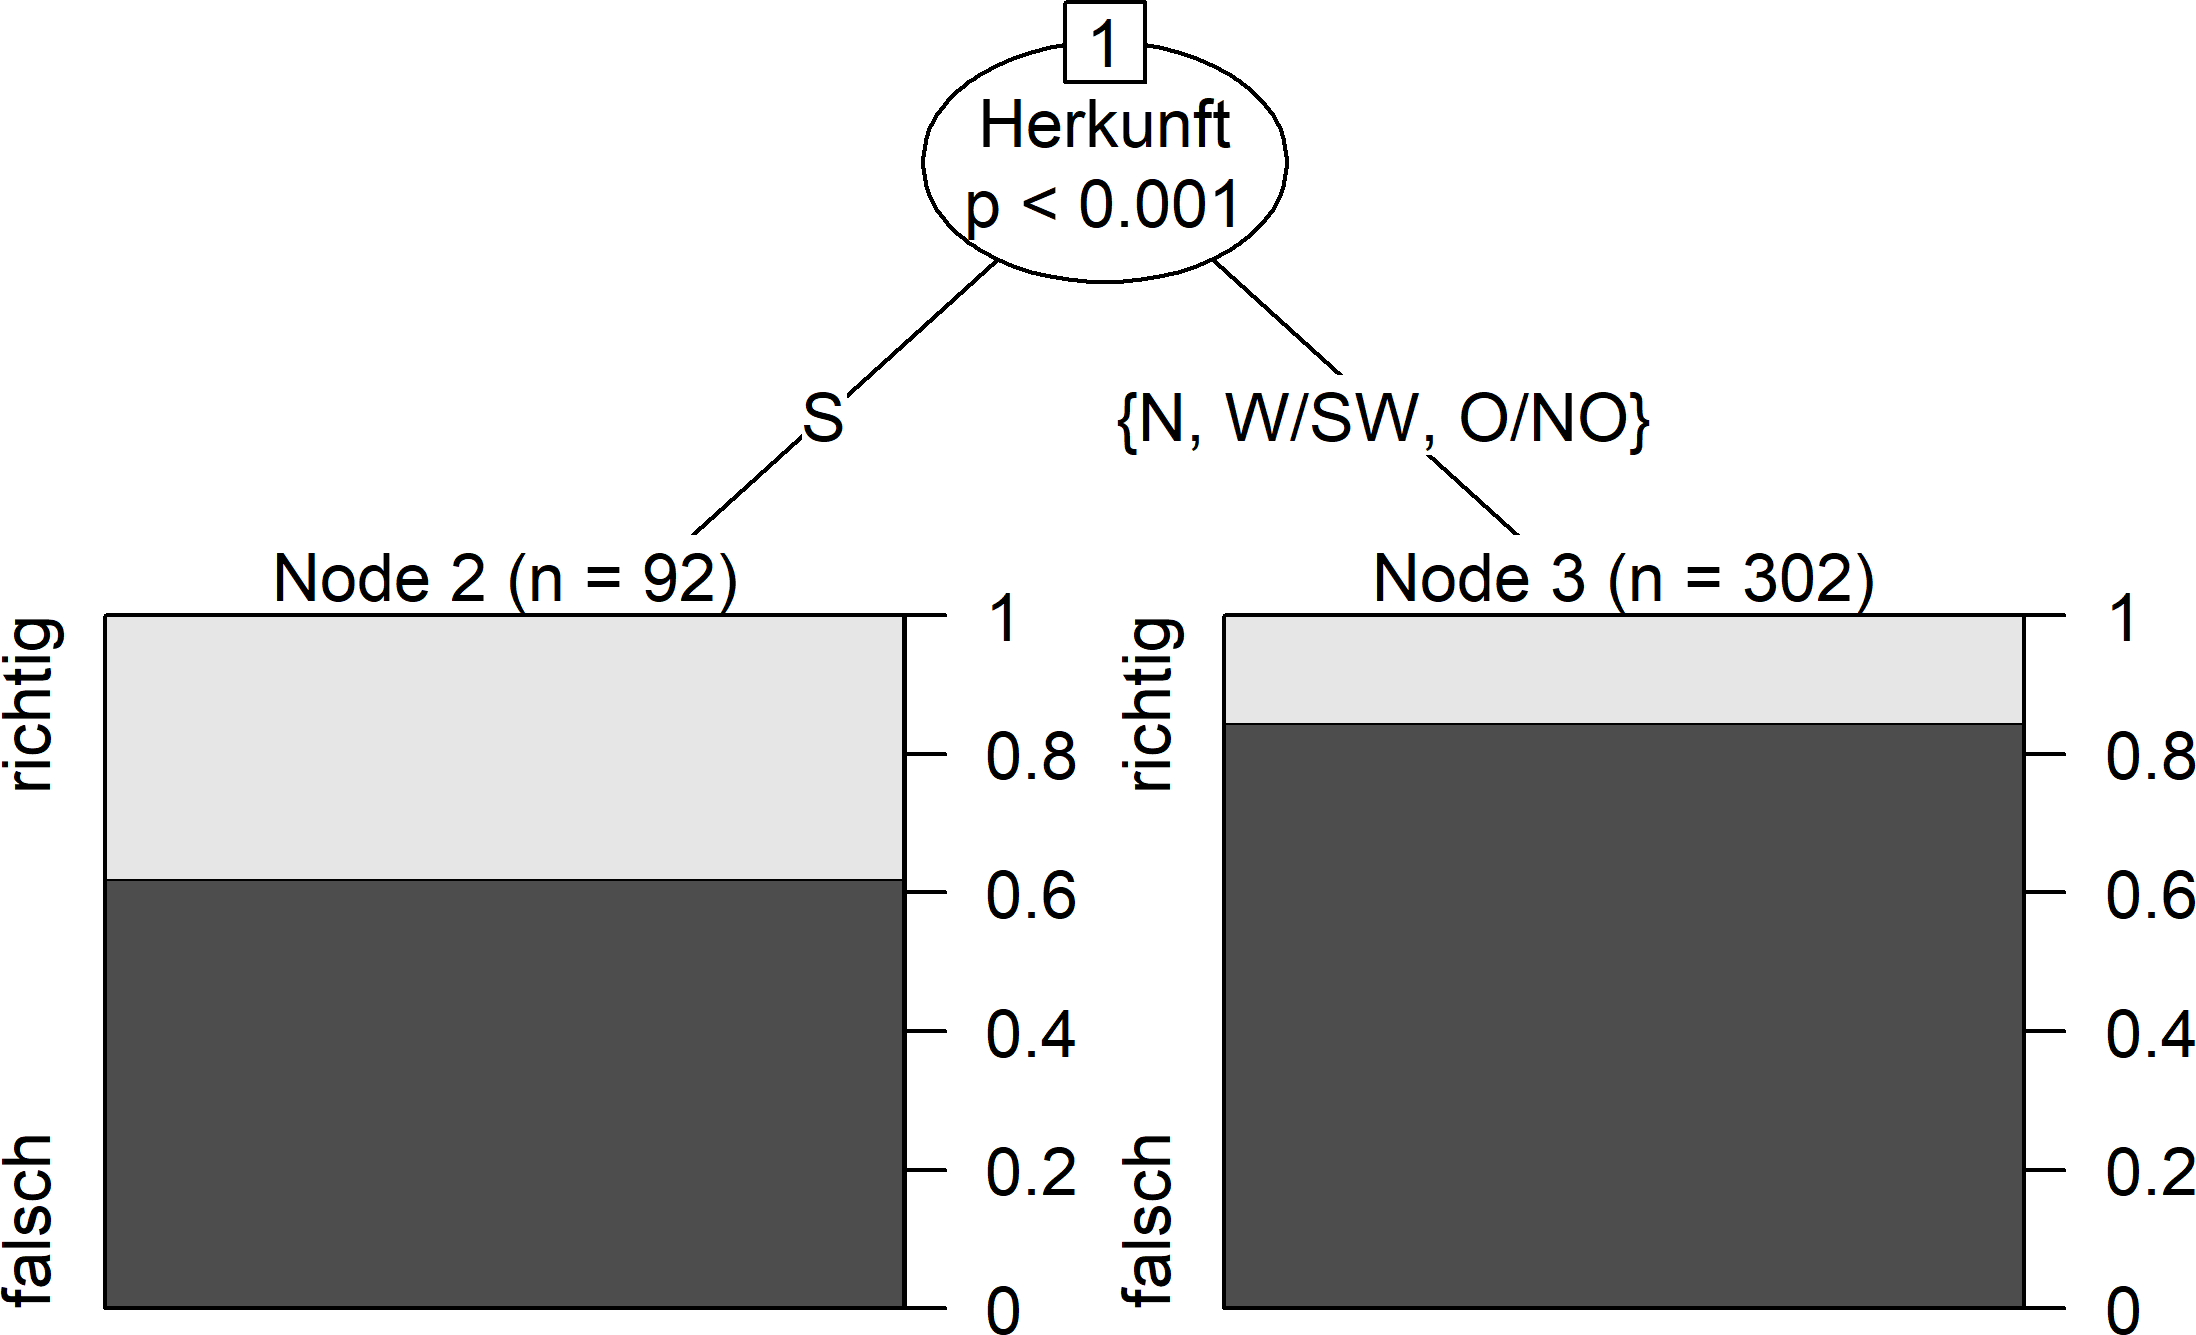
\includegraphics[width=\textwidth]{CtreeDativKorr.png}
\caption{\textit{Conditional Inference Tree} für die Bewertung der Korrektheit der Dativrektion bei \wegen{} und \waehrend}
\label{pic:CtreeKorrDativr}
\end{figure}

Der \textit{Conditional Inference Tree} zur Bewertung der Angemessenheit der Dativrektion bei \wegen{} und \waehrend{} splittet die Daten zunächst anhand des Settings (s. \autoref{pic:CtreeAngDativr}): 
Im formellen Kontext ist die Wahrscheinlichkeit für die Einstufung als unangemessen unter allen Befragten höher als im informellen Setting. 
Im informellen Setting hingegen urteilen norddeutsche Befragte dem Modell zufolge anders als Befragte aus dem restlichen Deutschland. 
%Änderung Anfang
Während für Norddeutsche eine Wahrscheinlichkeit von rund 0,5 vorhergesagt wird, dass sie die Variante auch in einem Gespräch mit einem Freund als unangemessen einstufen, ist unter den Befragten aus Süd-, West- bzw. Südwest und Ost- bzw. Nordostdeutschland die Wahrscheinlichkeit hoch, dass sie die Dativrektion hier als angemessen bewerten. 
% Änderung Ende
Mit einer \textit{Variable Importance} von 0,013 ist der Einfluss der Herkunft auf die Beurteilung der Angemessenheit allerdings deutlich geringer als der des Settings (\textit{Variable Importance} von 0,167). 
Die Passung des \textit{Random Forests} ist mit 0,92 sehr gut. 
\begin{figure}
\centering
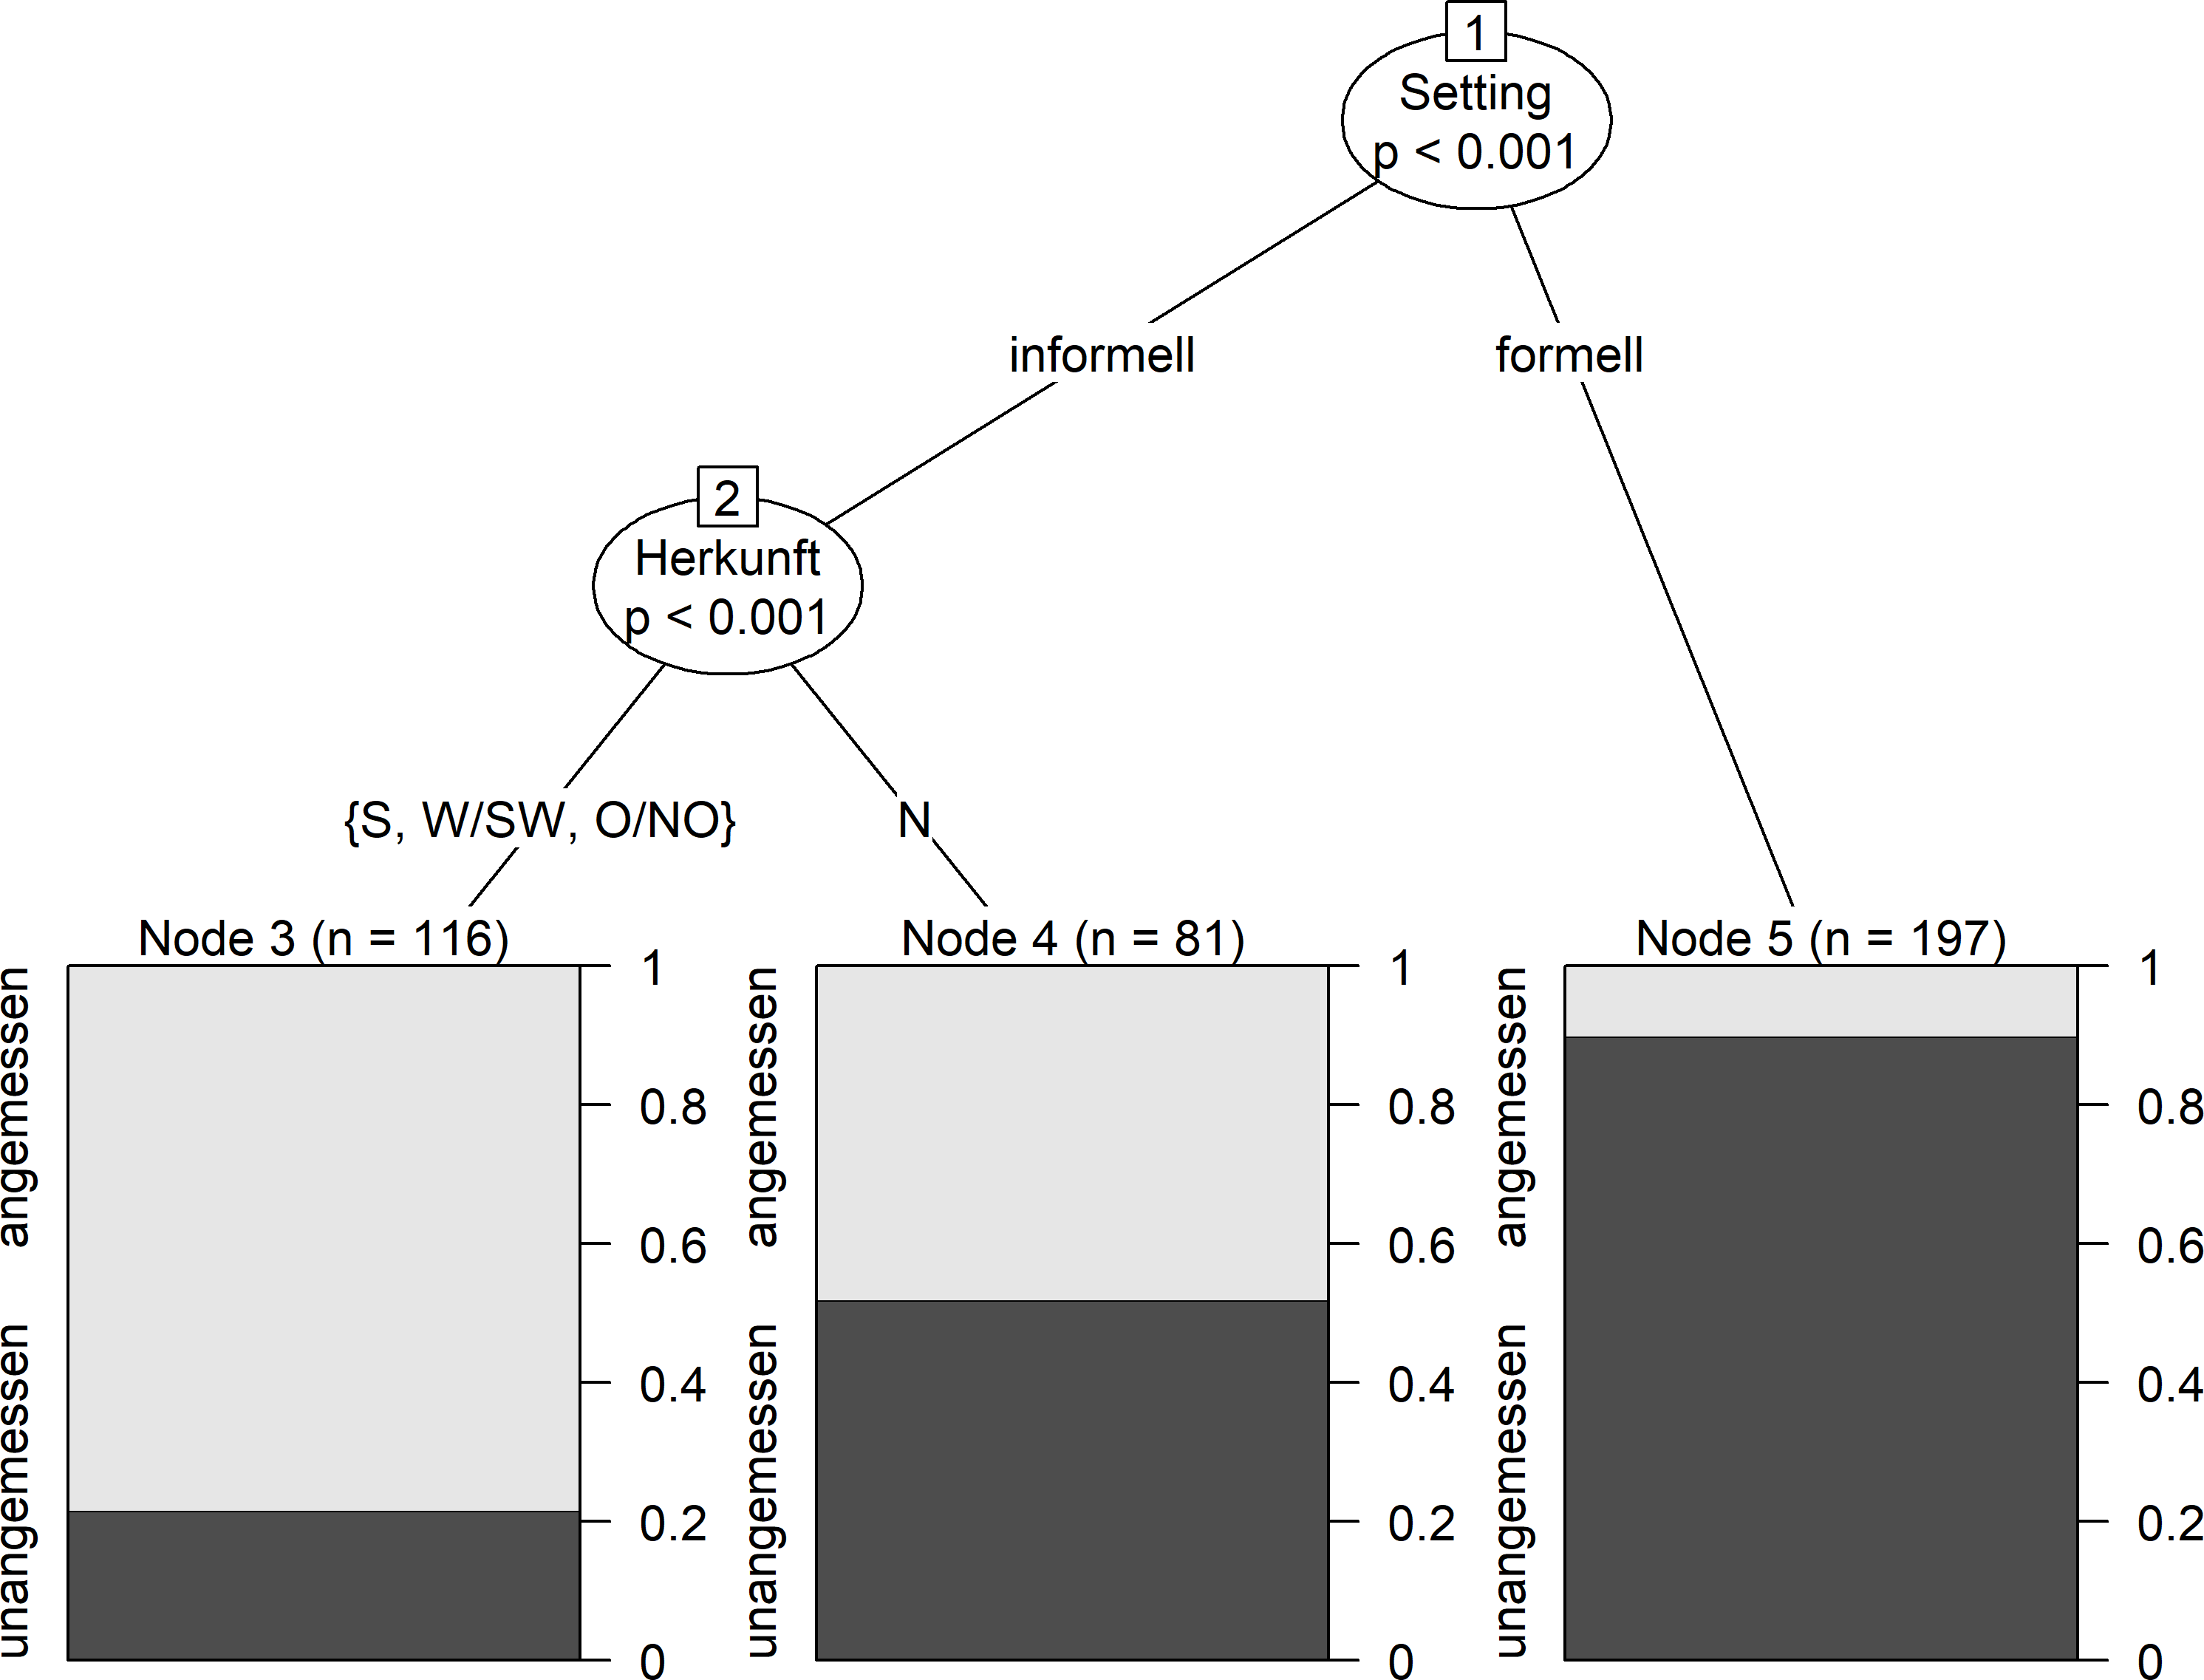
\includegraphics[width=\textwidth]{CtreeDativAng.png}
\caption{\textit{Conditional Inference Tree} für die Bewertung der Angemessenheit der Dativrektion bei \wegen{} und \waehrend}
\label{pic:CtreeAngDativr}
\end{figure}

Auch für die Angabe, ob Befragte die Dativrektion selbst verwenden würden, ist zunächst die Formalität des Settings ausschlaggebend (s. \autoref{pic:CtreeVerwDativr}). 
In einem Brief an ein Amt (formelles Setting) sagt das Modell für alle Befragten eine hohe Wahrscheinlichkeit voraus, den Dativ für die eigene Verwendung abzulehnen. 
Im informellen Setting spielt auch bei der Angabe zur eigenen Verwendung wieder die Herkunft eine Rolle (s. \textit{Node} 2). 
% Änderung Anfang
Dieses Mal stehen die Befragten aus süd- und west- bzw. südwestdeutschen Bundesländern den Befragten aus nord- und ost- bzw. nordostdeutschen Bundesländern gegenüber.
% Änderung Ende 
Für die Nord- und Ost- bzw. Nordostdeutschen sagt das Modell mit einer Wahrscheinlichkeit von rund 0,7 voraus, dass sie die Dativrektion auch im informellen Setting nicht verwenden würden. 
Bei Befragten aus Süd- und West- bzw. Südwestdeutschland hängt es von ihrer Variationstoleranz ab, wie wahrscheinlich es ist, dass sie den Dativ in einem informellen Kontext verwenden würden (s. \textit{Node} 3). 
Für Personen mit einer hohen Variationstoleranz wird mit einer Wahrscheinlichkeit von beinahe 0,9 vorausgesagt, dass sie \wegen{} oder \waehrend{} plus Dativ im Gespräch mit einem Freund verwenden würden. 
Für diejenigen Süd- und West- bzw. Südwestdeutschen, die Variation ablehnend gegenüberstehen, sagt das Modell dies nur mit einer Wahrscheinlichkeit von rund 0,5 vorher. 
Die vom \textit{Random Forest} berechneten \textit{Variable Importances} legen nahe, dass der Einfluss des Settings (0,079) deutlich größer ist als der von Herkunft (0,037) und Variationstoleranz (0,01). 
Der C-Wert beträgt 0,91 und zeigt damit eine sehr gute Passung des Modells auf die Daten an. 
\begin{figure}[p]
\centering
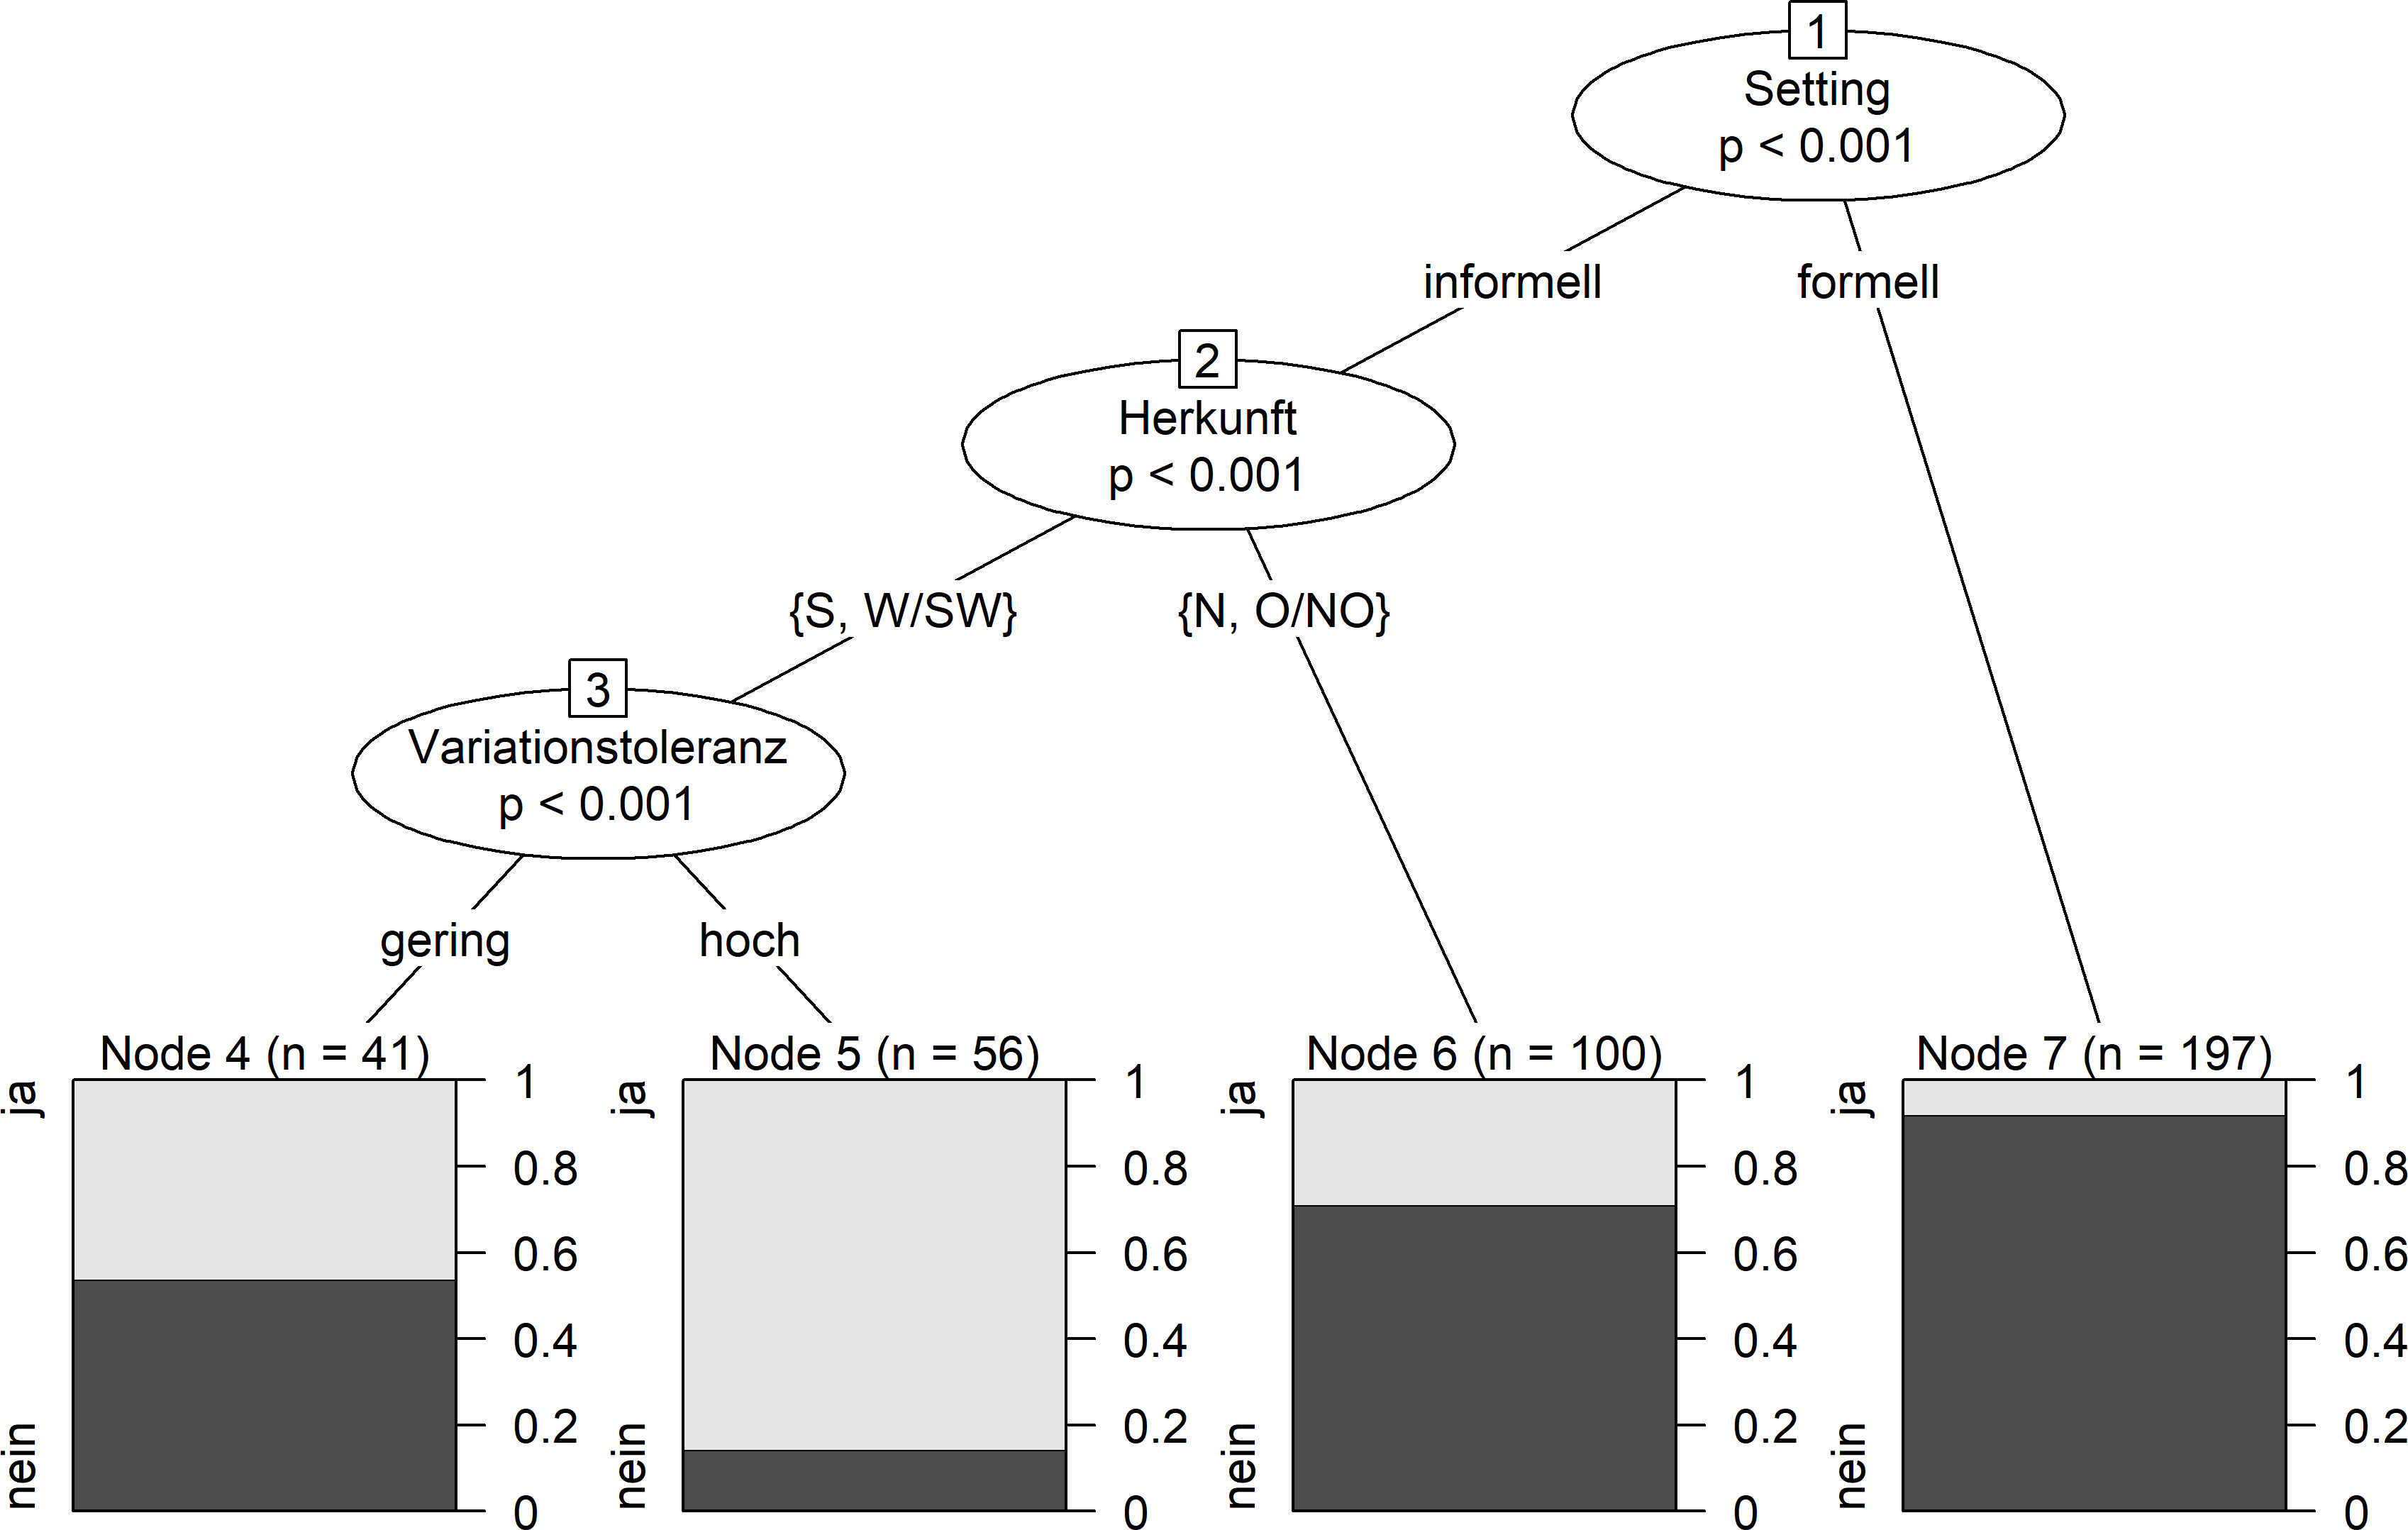
\includegraphics[angle=90, scale=0.7]{CtreeDativVerw.png}
\caption{\textit{Conditional Inference Tree} für die Angaben zur eigenen Verwendung der Dativrektion bei \wegen{} und \waehrend}
\label{pic:CtreeVerwDativr}
\end{figure}

Die \textit{Conditional Inference Trees} zur Genitivrektion bei \dank{} zeigen keinen Split in den Daten.
Alle von den \textit{Random Forests} berechneten \textit{Variable Importances} liegen bei oder sehr nahe bei null.
Das heißt, die Angaben zur Korrektheit, Angemessenheit und eigenen Verwendung von \dank{} plus Genitiv zeigen keine Abhängigkeit von einer der getesteten Variablen. 
Offenbar beurteilen Befragte die Variante unabhängig vom Setting, ihrem Alter, ihrer regionalen Herkunft, ihrem Bildungsstand, der Textaffinität ihres Berufs und ihrer Variationstoleranz häufig als korrekt und angemessen und würden sie selbst verwenden (\autoref{sec:ErgAkzNachAlter} bis \autoref{sec:ErgAkzNachVT}). 
Die C-Werte für die drei \textit{Random Forests} betragen alle über 0,8 und repräsentieren die Daten damit gut.

\object{Gegenüber} wird im Akzeptabilitätstest unabhängig von den getesteten Variablen eher abgelehnt. 
Auch hier werden die Daten von den \textit{Conditional Inference Trees} nicht aufgeteilt. 
Die Passung der \textit{Random Forests} liegt jeweils bei mindestens 0,8, ist also gut. 
Die grafischen Darstellungen der \textit{Conditional Inference Trees} zu \dank{} und \gegenueber{} finden sich im Anhang (s. \autoref{pic:AnhCtreeKorrGenitivrDank} bis \autoref{pic:AnhCtreeVerwGenitivrGegenueber}). 

\autoref{pic:CtreeKorrGenitivrSeit} zeigt den \textit{Conditional Inference Tree} für die Bewertung der Korrektheit der Genitivrektion bei der Primärpräposition \object{seit}.
Er splittet die Daten anhand der Variable \glqq Textaffinität des Berufs\grqq:
Für Befragte aus textaffinen Berufen wird eine geringere Wahrscheinlichkeit vorhergesagt, dass sie \object{seit} plus Genitiv als korrekt beurteilen. 
Der \textit{Random Forest} gibt für die Textaffinität des Berufs eine \textit{Variable Importance} von 0,008 an. 
Im Vergleich dazu liegt der Wert für den Faktor \glqq Altersgruppe\grqq, der keinen Split im \textit{Tree} erzeugt, nur bei 0,004.
Mit einem C-Wert von 0,8 passt das Modell gut auf die Daten. 
\begin{figure}
\centering
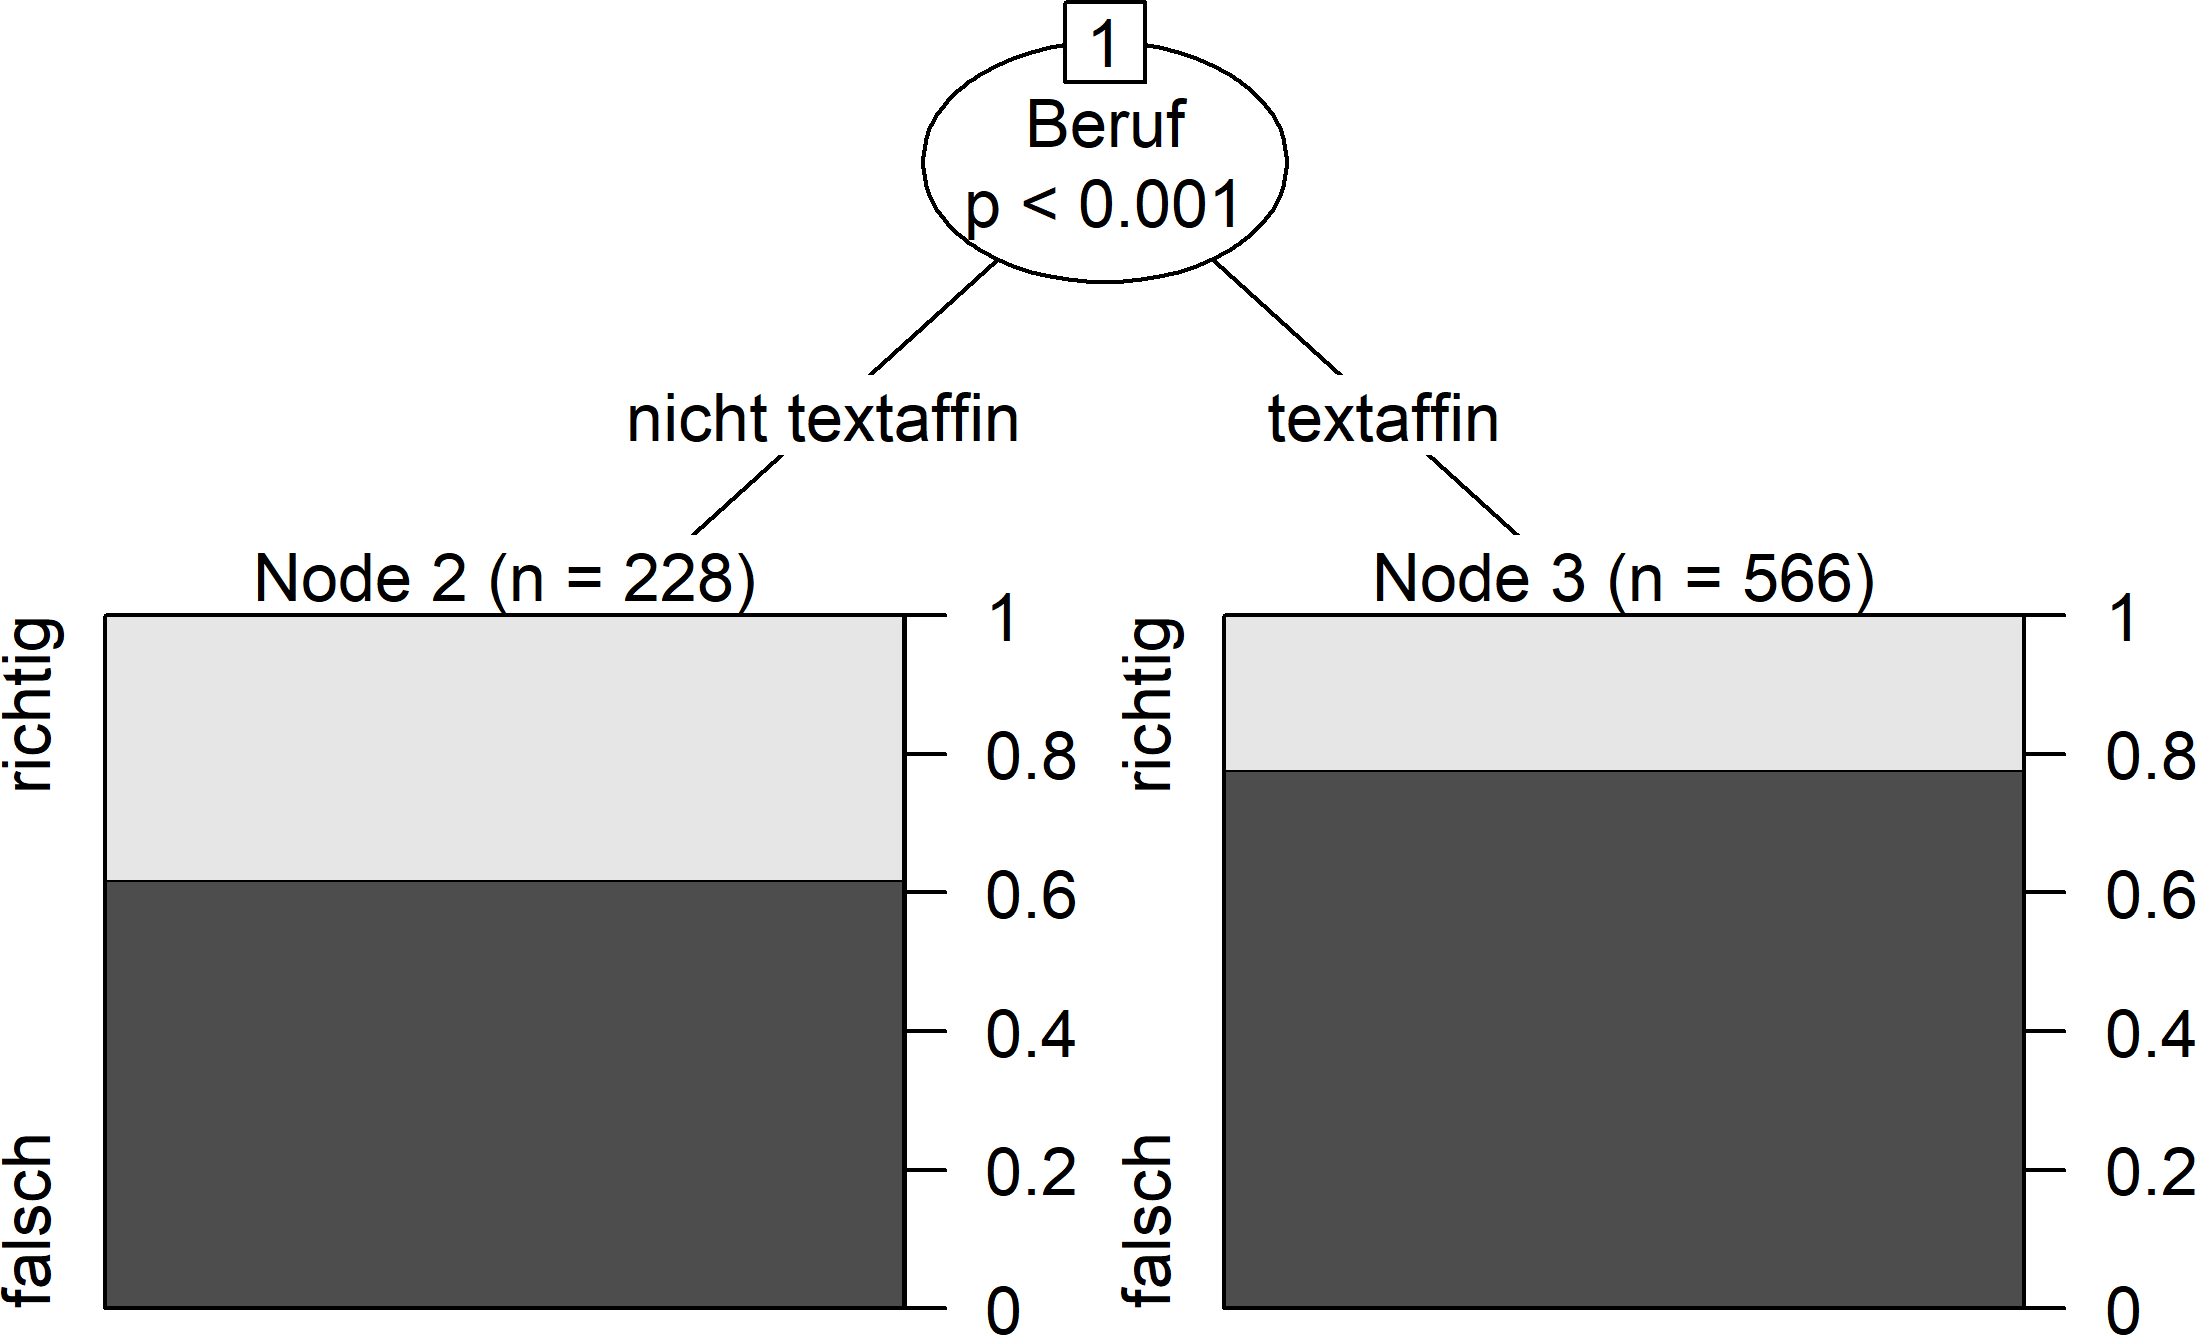
\includegraphics[width=\textwidth]{CtreeGenitivseitKorr.png}
\caption{\textit{Conditional Inference Tree }für die Bewertung der Korrektheit der Genitivrektion bei \object{seit}}
\label{pic:CtreeKorrGenitivrSeit}
\end{figure}

Auch der \textit{Conditional Inference Tree} zur Beurteilung der Angemessenheit von \object{seit} mit dem Genitiv splittet die Daten anhand der Textaffinität des Berufs, wie in \autoref{pic:CtreeAngGenitivrSeit} zu sehen. 
Allerdings liegt die \textit{Variable Importance} der Textaffinität des Berufs hier mit 0,004 sehr nah an der der anderen Faktoren, für die kein Split erzeugt wird. 
Über viele Baummodelle gemittelt scheint sich ihr Einfluss also zu relativieren. 
Der \textit{Random Forest} für die Beurteilung der Angemessenheit von \object{seit} plus Genitiv hat mit 0,81 eine gute Passung. 
\begin{figure}
\centering
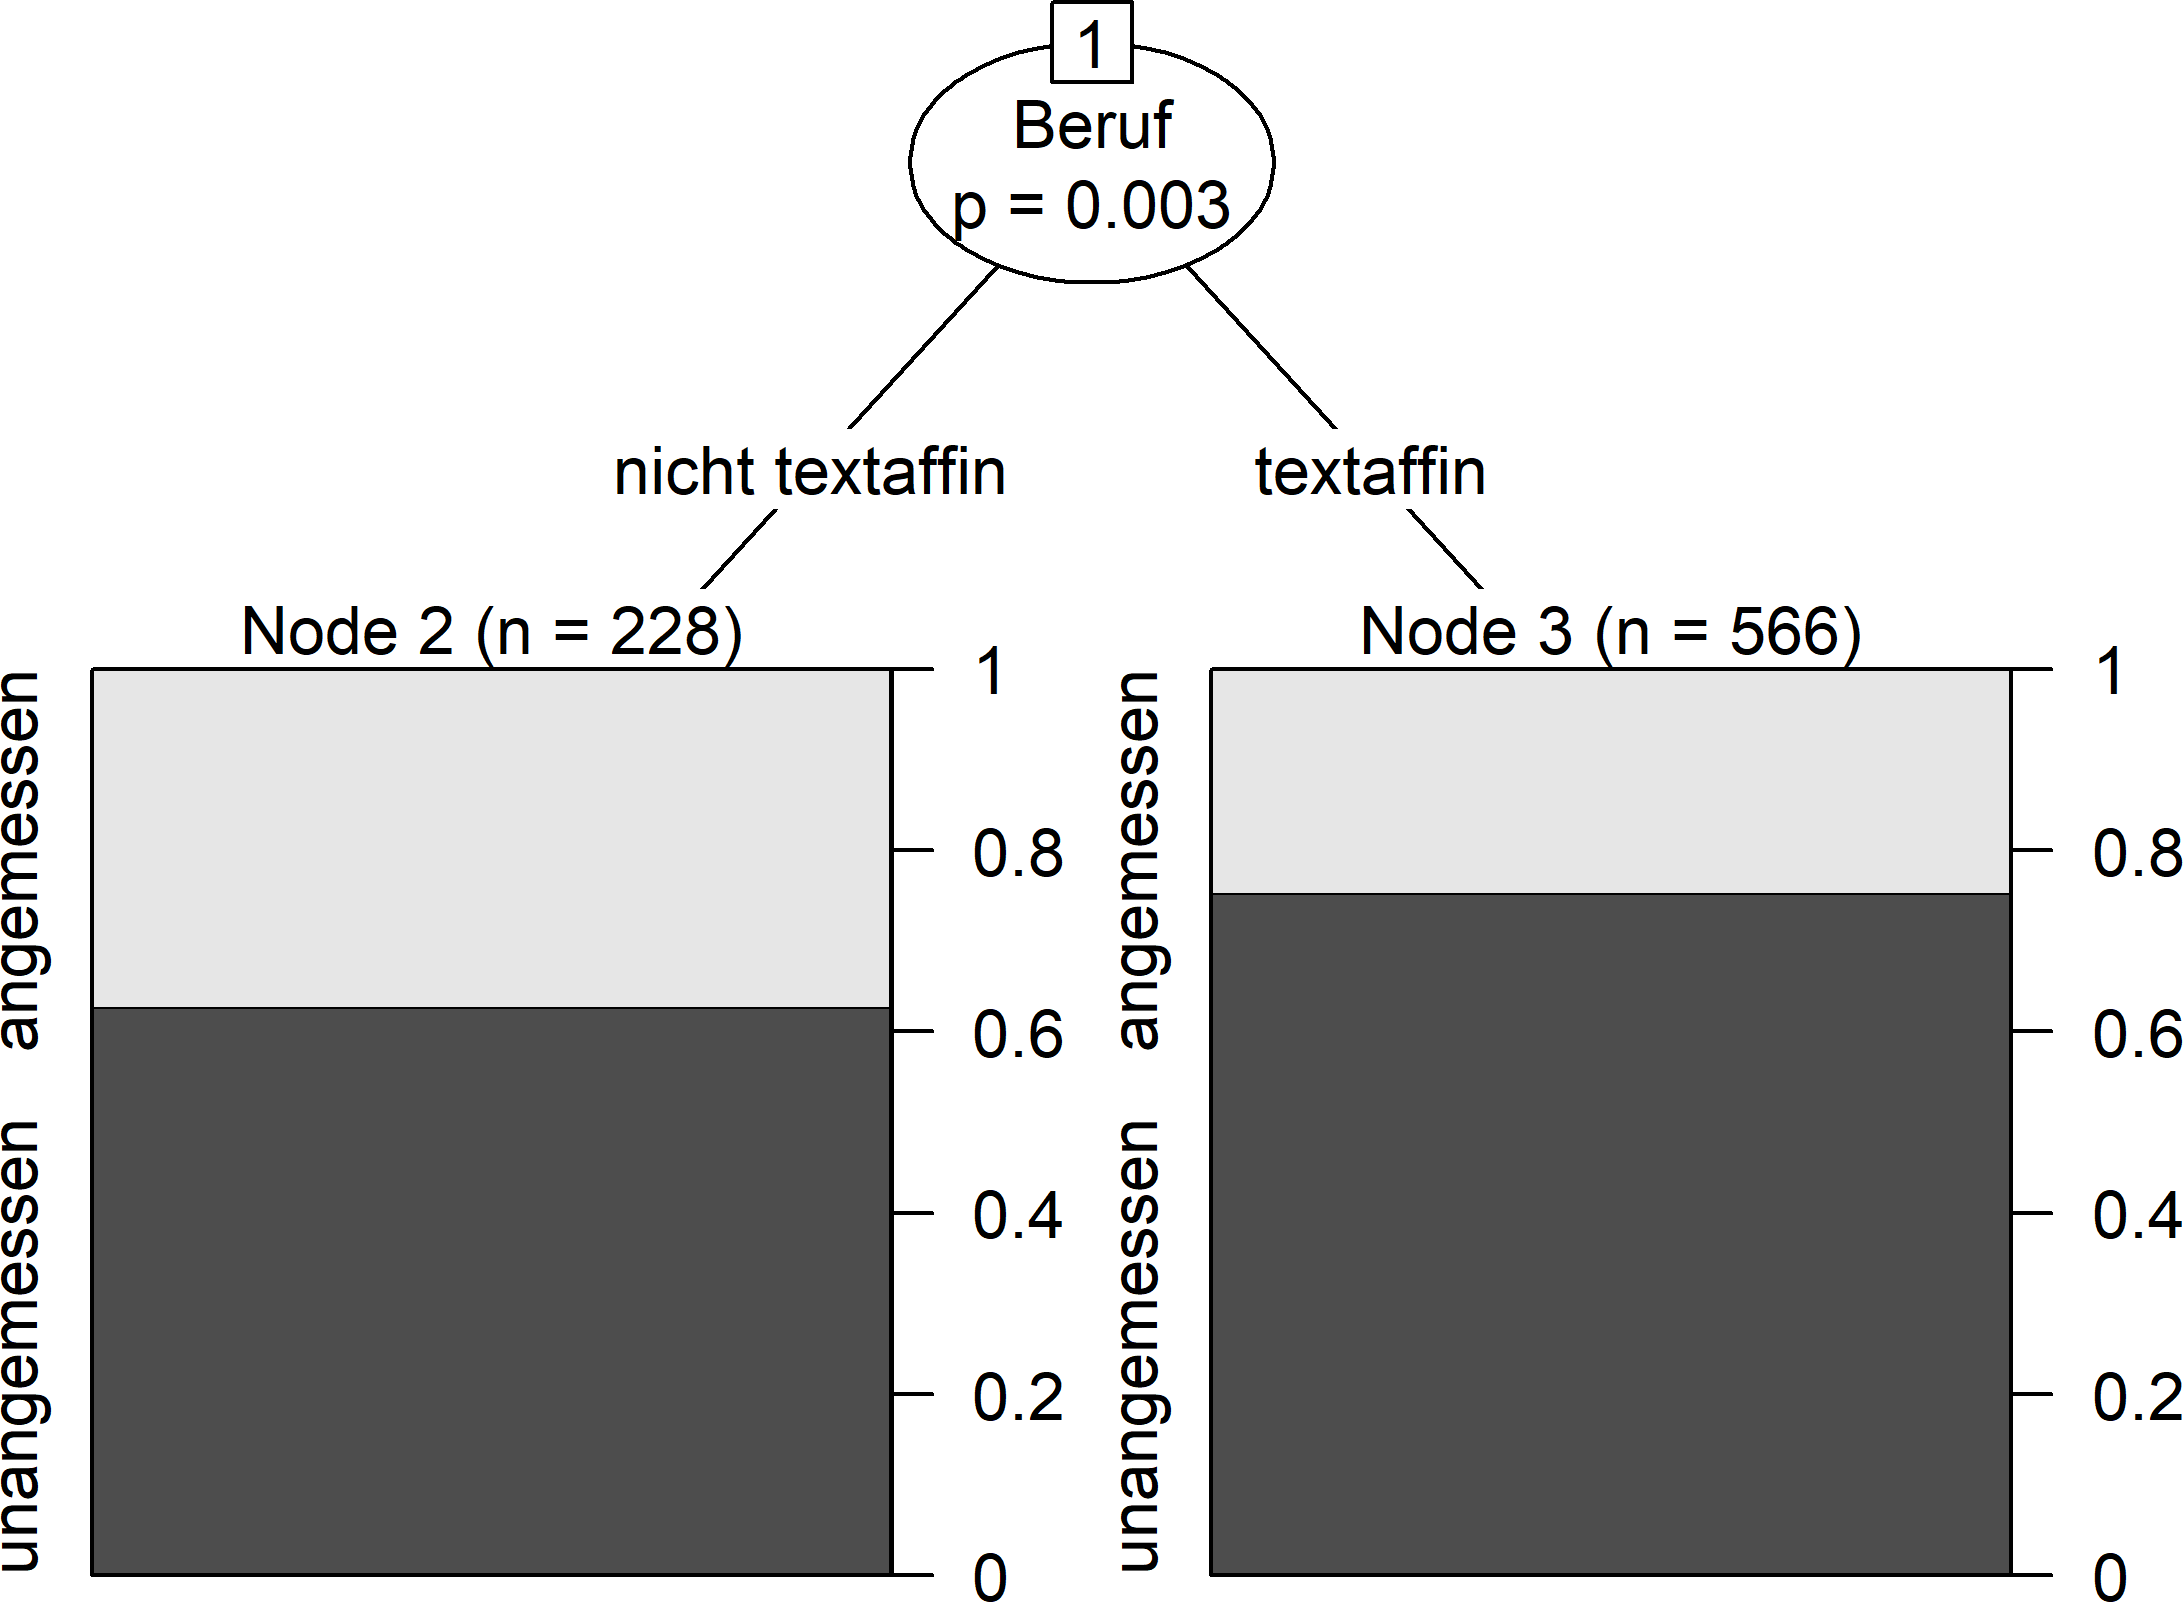
\includegraphics[width=\textwidth]{CtreeGenitivseitAng.png}
\caption{\textit{Conditional Inference Tree} für die Bewertung der Angemessenheit der Genitivrektion bei \object{seit}}
\label{pic:CtreeAngGenitivrSeit}
\end{figure}

In \autoref{pic:CtreeVerwGenitivrSeit} ist der \textit{Conditional Inference Tree} für die Angaben zur eigenen Verwendung der Genitivrektion bei der Primärpräposition \object{seit} dargestellt. 
Der erste Split in den Daten wird hier anhand des Settings erzeugt. 
Anschließend werden die Daten im formellen Setting nach der Textaffinität des Berufs geteilt (s. \textit{Node} 2) und im informellen Setting nach dem Bildungsstand der Befragten (s. \textit{Node} 5). 
Die höchste Wahrscheinlichkeit für die Angabe, die Variante selbst zu verwenden, sagt das Modell für Befragte aus nicht-sprachaffinen Berufen im formellen Setting vorher (s. \textit{Node} 3). 
Für Befragte mit Hochschulabschluss im informellen Setting hingegen ist die Wahrscheinlichkeit, dass sie angeben, \object{seit} plus Genitiv selbst zu verwenden, am geringsten (s. \textit{Node} 7). 
% Änderung Anfang
Höherer Bildungsgrad und höhere Textaffinität des Berufs gehen also mit niedrigeren Werten zur Selbsteinschätzung der Verwendung des Genitivs bei \textit{seit} einher. 
% Änderung Ende
Schaut man sich jedoch die vom \textit{Random Forest} berechneten \textit{Variable Importances} an, liegen diese für die Textaffinität des Berufs und den Bildungsstand mit 0,003 und 0,002 höher als für das Setting und insgesamt sehr nah bei null.
Das Setting hat mit 0,002 eine ebenso hohe \textit{Variable Importance} wie der Faktor \glqq Altersgruppe\grqq, der im \textit{Tree} nicht zu einem Split führt. 
Dies deutet auf eine geringe Aussagekraft des Modells hin. 
Die Passung des \textit{Random Forests} ist mit 0,84 dennoch gut. 
\begin{figure}[p]
\centering
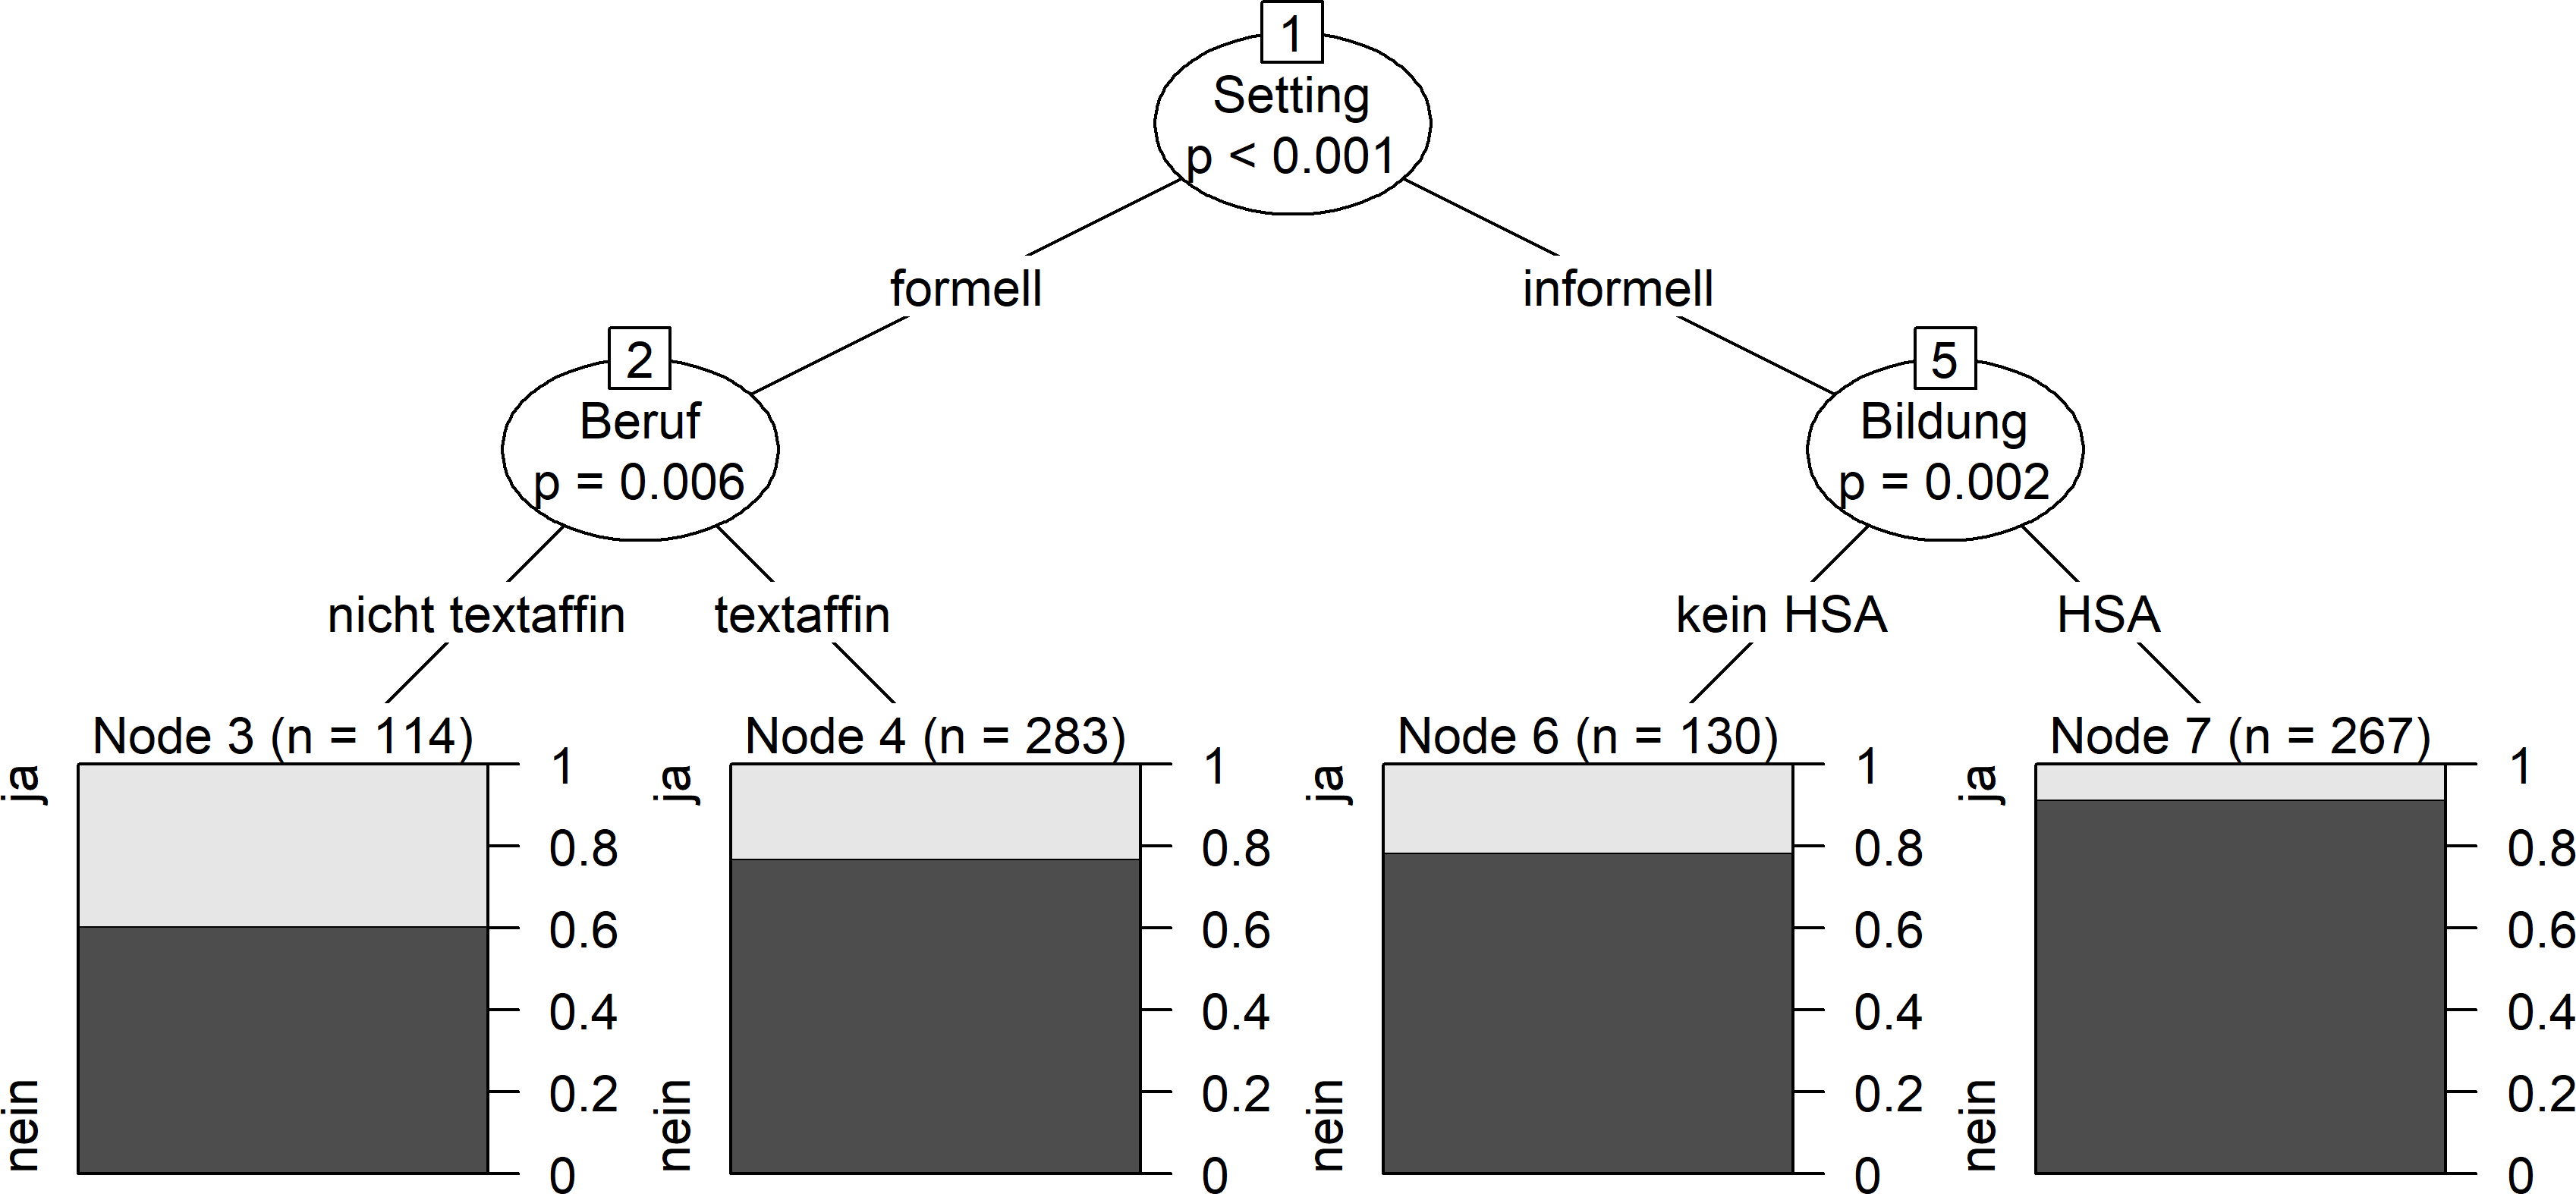
\includegraphics[angle=90, scale=0.75]{CtreeGenitivseitVerw.png}
\caption{\textit{Conditional Inference Tree} für die Angaben zur eigenen Verwendung der Genitivrektion bei \object{seit}}
\label{pic:CtreeVerwGenitivrSeit}
\end{figure}
 Die statistische Analyse der Daten aus dem Akzeptabilitätstest macht deutlich, dass die Bewertung der Dativrektion bei \wegen{} und \waehrend{} insbesondere von der Formalität des Settings und von der Herkunft der Befragten abhängt.
Auf die Angabe, ob Befragte die Variante selbst verwenden würden, hat außerdem ihre Variationstoleranz einen geringen Einfluss. 
Die Beurteilung der Genitivrektion bei \dank{} und \gegenueber{} zeigen keine Abhängigkeit von den hier getesteten Variablen.
Für die Bewertung der Korrektheit und Angemessenheit der Genitivrektion bei der Primärpräposition \object{seit} werden unterschiedliche Wahrscheinlichkeiten vorhergesagt, je nachdem, ob Befragte einen textaffinen Beruf haben.  
\subsection{Begründungen für die Unangemessenheit einer Variante}
\label{sec:Begruendungen}
% Begründungen
Bisher wurden die Antworten auf die geschlossenen Fragen im Akzeptabilitätstest ausgewertet. 
Der folgende Abschnitt widmet sich den Antworten auf die offene Frage nach dem Grund für die Einstufung als unangemessen: 
Wenn die Befragten eine Variante im Akzeptabilitätstest als unangemessen bewerteten, wurden sie mit der Frage \glqq was stört Sie?\grqq{} um eine Begründung gebeten (\autoref{sec:Akz}). 

Die Begründungen für die Ablehnung von \wegen{} oder \waehrend{} plus Dativ sowie von \dank{} oder \gegenueber{} plus Genitiv wurden analog zu den freien Assoziationen (\autoref{sec:ErgAss}) inhaltsanalytisch ausgewertet.\footnote{Begründungen für die Beurteilung des Genitivs bei der Primärpräposition \object{seit} als unangemessen wurden ebenfalls erhoben, werden aber nicht im Rahmen dieser Untersuchung ausgewertet.}
Das dafür genutzte Kategoriensystem basiert auf dem für die Assoziationen erstellten. 
Daher soll an dieser Stelle lediglich auf die Anpassungen eingegangen werden, die im Zuge des ersten Kodierungsdurchgangs an einem repräsentativen Sample der Daten erfolgt sind (zum genauen Vorgehen bei der Kategorisierung s. \autoref{sec:Akz}). 
Das Handbuch für die Kodierung der Begründungen im Akzeptabilitätstest findet sich im Anhang (\autoref{Anh:HandbuchBegr}). 
Als Kodierungseinheit diente, wie schon bei den Assoziationen, jeweils die gesamte Antwort eines/r Befragten. 
Wenn eine Antwort verschiedene Begründungen anführte, wurde sie in mehrere Kategorien einsortiert. 
%Die Schritte bei der Kategorisierung der Begründungen entsprechen denen bei der Kategorisierung der Assoziationen: 
%Nach dem ersten Kodierungsdurchgang an einem Teil der Daten wurde ein Kodierungshandbuch erstellt. 
%Anschließend wurde der komplette Datensatz zweimal in \citet{MAXQDA.19892018} kodiert, sodass die Intracoderreliabilität berechnet werden konnte.
%Ein repräsentatives Viertel der Antworten wurde auch hier zusätzlich von zwei Hilfskräften kodiert, was auch eine Kontrolle der Intercoderreliabilität zulässt. 

Für die Kodierung der Begründungen im Akzeptabilitätstest stehen insgesamt 17 Oberkategorien zur Verfügung, die sich größtenteils mit den Oberkategorien für die freien Assoziationen decken. 
Hinzugekommen sind lediglich zwei Kategorien:
Erstens die Kategorie \glqq nur Vorschlag/Benennung\grqq{} für Antworten, die keine Begründung enthalten, sondern nur auf die sprachliche Form verweisen, was zur Einstufung als unangemessen geführt hat, oder die stattdessen bevorzugte Form nennen. 
Beispiele für diese Art von Antworten sind die folgenden: 
\begin{exe}
\ex \object{Fehlender Genitiv} (Behördenangestellter, 56, zu \waehrend{} mit dem Dativ im formellen Setting)
\ex \object{Der Kasus} (Hotelrezeptionistin, 30, zu \dank{} mit dem Genitiv im formellen Setting)
\ex \object{Gegenüber dem Sachbearbeiter} (Lehramtsstudentin, 24, zu \gegenueber{} mit dem Genitiv im formellen Setting)
\end{exe}
Die zweite Oberkategorie, die hinzugekommen ist, ist die Kategorie \glqq Sprachgefühl\grqq, da es Antworten gibt, in denen Befragte ihre eigene sprachliche Intuition als Begründung für die Ablehnung einer Variante heranziehen, wie etwa hier:
\begin{exe}
\ex \object{eher während des Vortrags. Das klingt für mich besser} (Biologiedoktorandin, 25, zu \waehrend{} mit dem Dativ im formellen Setting)
\end{exe}
Da in den Begründungen aus dem Akzeptabilitätstest nie auf die Stellung einer Präposition Bezug genommen wird, fehlt die Oberkategorie \glqq Stellung\grqq{} in dem angepassten Kategorienset. 
Insgesamt stehen für die Kodierung der Begründungen für die Bewertung einer Variante als unangemessen folgende Oberkategorien zur Verfügung: \glqq Personentypus\grqq, \glqq eigener Gebrauch\grqq, \glqq Sprachgefühl\grqq, \glqq Zweifel\grqq, \glqq Formalität\grqq, \glqq Medium\grqq, \glqq Varietät\grqq, \glqq Korrektheit\grqq, \glqq Gleichgültigkeit\grqq, \glqq Ästhetik\grqq, \glqq Sprachwandel\grqq, \glqq Bedeutung und Verständlichkeit\grqq, \glqq Herleitung\grqq, \glqq nur Vorschlag/Benennung\grqq, \glqq nicht relevant\grqq, \glqq keine Angabe\grqq{} und \glqq nicht entscheidbar\grqq. 
Die Kategorie \glqq nicht relevant\grqq{} wurde für Antworten vergeben, in denen deutlich wird, dass die Unangemessenheit der Form nicht am Kasus festgemacht wird. 
Ein Beispiel dafür ist folgende Antwort: 
\begin{exe}
\ex \object{Name des Sachbearbeiters fehlt} (Chemielaborant, 27, zu \gegenueber{} mit dem Genitiv im formellen Setting)
\end{exe}
In die Kategorie \glqq keine Angabe\grqq{} fallen Antworten wie \object{nichts} oder \object{keine Ahnung}. 
\glqq Nicht entscheidbar\grqq{} wurde vergeben, wenn die Begründung unklar war, etwa bei Antworten wie \object{Grammatik} oder \object{Ausdruck}. 

Insgesamt liegen bei den Begründungen für die Unangemessenheit einer Variante deutlich weniger Antworten vor als bei den freien Assoziationen.
Dies liegt daran, dass nur diejenigen Befragten nach einer Begründung gefragt wurden, die eine Variante als unangemessen abgelehnt haben.  
In \autoref{pic:OKatBegr} ist zu sehen, wie viele Antworten in den 17 Oberkategorien jeweils kodiert wurden. 

\begin{figure}
\centering
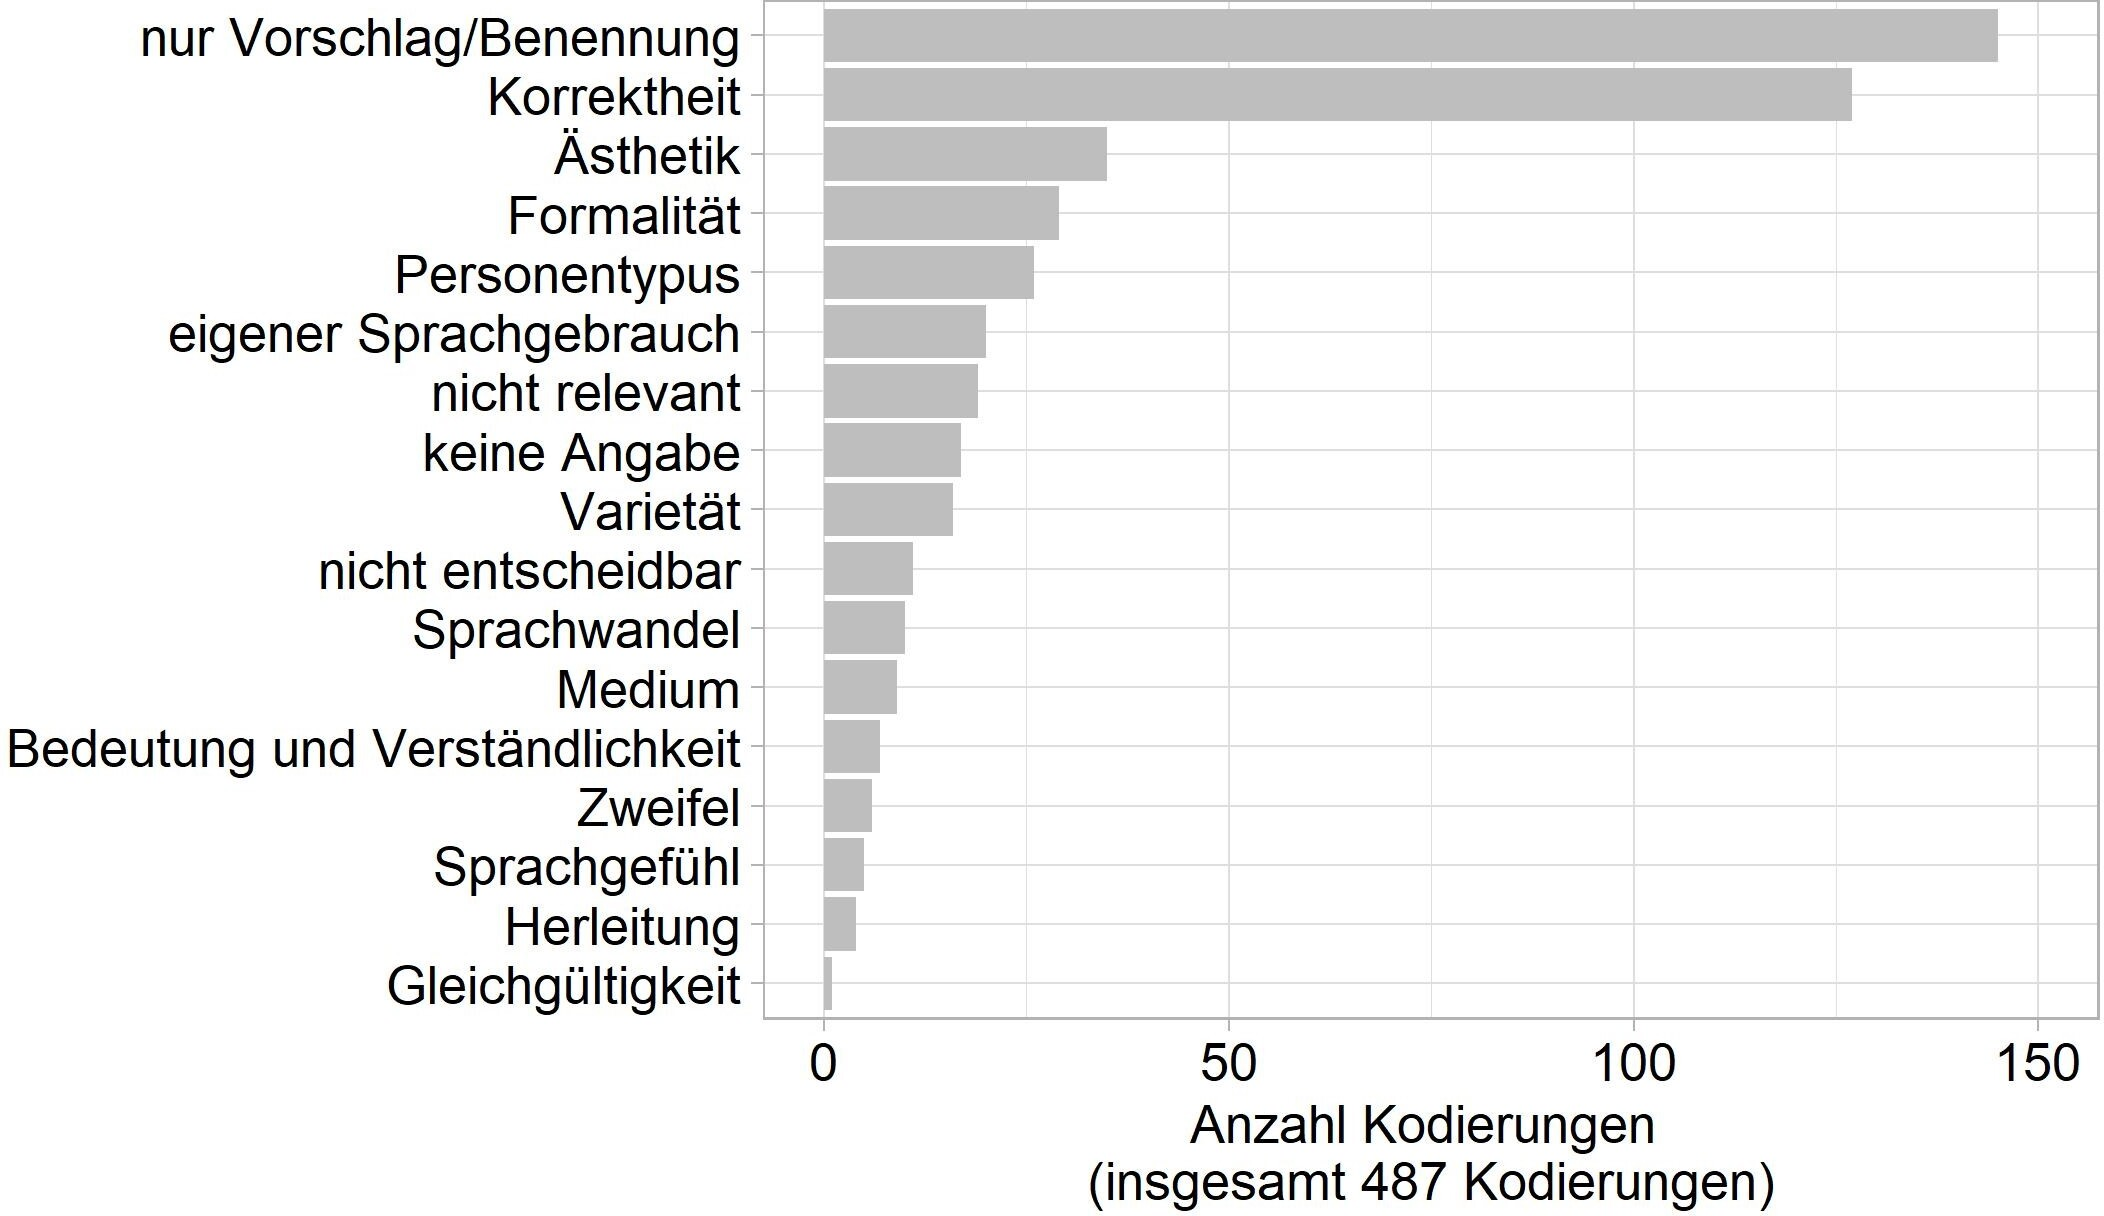
\includegraphics[width=\textwidth]{OKatBegr.jpg}
\caption{Anzahl der Kodierungen von Begründungen für die Unangemessenheit einer Variante in den Oberkategorien}
\label{pic:OKatBegr}
\end{figure}

Die Kategorie \glqq nur Vorschlag/Benennung\grqq{} ist am häufigsten vertreten:
145 Antworten enthalten lediglich einen Vorschlag oder benennen die unangemessene Form. 
Dass die meisten Befragten auf diese Art und Weise antworten, liegt an der Elizitation der Antworten durch die Frage \glqq was stört Sie?\grqq. 
Umso interessanter ist es, dass zahlreiche Befragte ihre Entscheidung auch begründen. 
Am häufigsten wird die Korrektheit bzw. Inkorrektheit einer Variante als Begründung angeführt. 
Neben \glqq nur Vorschlag/Benennung\grqq{} ist \glqq Korrektheit\grqq{} die mit Abstand häufigste Kategorie.  
127 Antworten begründen die Entscheidung im Akzeptabilitätstest über die (In)Korrektheit der Form. 
Dies zeigt, dass Angemessenheit und Korrektheit einer Variante für viele Befragte in einem engen Zusammenhang stehen. 
Die nächsthäufigen Begründungskategorien sind \glqq Ästhetik\grqq{} (35 Antworten), \glqq Formalität\grqq{} (29 Antworten) und \glqq Personentypus\grqq{} (26 Antworten). 
Alle anderen Kategorien haben höchstens 20 Vorkommnisse und scheinen damit für die Begründung, warum eine Variante als unangemessen eingestuft wurde, weniger relevant zu sein. 
Im Folgenden sollen die vier häufigsten Begründungskategorien, \glqq Korrektheit\grqq, \glqq Ästhetik\grqq, \glqq Formalität\grqq{} und \glqq Personentypus\grqq{} genauer betrachtet werden. 

%\subsection{Begründungen über Korrektheit}
Da im Akzeptabilitätstest danach gefragt wurde, was an dem Beispiel stört, wurde in den Antworten beinahe nie angemerkt, dass eine Form richtig sei. 
121 der 127 Antworten aus der Oberkategorie \glqq Korrektheit\grqq{} bezeichnen die Beispielvariante als falsch: 
\begin{exe}
\ex \object{verkehrter Fall} (Wissenschaftlicher Mitarbeiter Ingenieurwissenschaft, 26, zu \gegenueber{} mit dem Genitiv im formellen Setting) 
\ex \object{Grammatikfehler} (Geschichts- und Mathematiklehrer, 65, zu \waehrend{} mit dem Dativ im informellen Setting) 
\end{exe}
Neben solchen Beispielen, die eine Form explizit als inkorrekt benennen, wurden in \glqq Korrektheit > falsch\grqq{} auch Antworten kodiert, die dies impliziter tun, wie etwa die folgende:
\begin{exe}
\ex \object{Es heißt: während des Vortrags} (Oberstudienrat für Latein und Sport, 50, zu \waehrend{} mit dem Dativ im formellen Setting) 
\end{exe}
Indem die Genitivvariante hier mit \object{es heißt} kategorisch als richtig dargestellt wird, wird der Dativvariante die Korrektheit gleichzeitig abgesprochen. 

Die wenigen Antworten, die eine Variante als richtig bezeichnen, machen meist eine einschränkende Aussage, wie etwa diese Beispiele zeigen: 
\begin{exe}
\ex \object{Benutzt kaum jemand mehr, obwohl es noch korrekt ist} (Lehramtsstudentin, 24, zu \dank{} mit dem Genitiv im informellen Setting) \label{Bsp:BegrKorr1}
\ex \object{leider ist vermutlich beides laut Duden richtig} (Hauptschullehrer, 69, zu \wegen{} mit dem Dativ im formellen Setting) \label{Bsp:BegrKorr2}
\end{exe}
In \autoref{Bsp:BegrKorr1} wird \dank{} plus Genitiv im informellen Setting als unangemessen beurteilt. 
Die Befragte begründet diese Entscheidung damit, dass die Variante zwar richtig sei, jedoch kaum verwendet würde. 
Mit \object{mehr} und \object{noch} drückt sie zudem ihre Annahme aus, dass hier ein Sprachwandel stattfindet, bei dem die Genitivrektion zugunsten der Dativrektion weicht. 
In \autoref{Bsp:BegrKorr2} wird die Vermutung geäußert, dass der Duden bei \wegen{} sowohl die Genitiv- als auch die Dativrektion lizensiert. 
Darüber wird durch \object{leider} Bedauern ausgedrückt, wodurch deutlich wird, dass der Befragte die Dativrekion ablehnt, obwohl er davon ausgeht, dass sie laut kodifizierter Norm korrekt ist. 

\autoref{pic:BegrKorrektheit} zeigt die quantitative Verteilung der Begründungen, die auf die Korrektheit bzw. Inkorrektheit einer Variante verweisen, im Vergleich zu anderen Begründungen: 
Ein Balken bildet jeweils ab, wie häufig eine Variante insgesamt als unangemessen eingestuft wird. 
In Blautönen ist dargestellt, wie häufig diese Einstufung mit der (In-)Korrektheit der Variante begründet wird. 
Die grauen Bereiche der Balken machen sichtbar, wie häufig andere Begründungen bei einer Variante sind. 
\begin{figure}
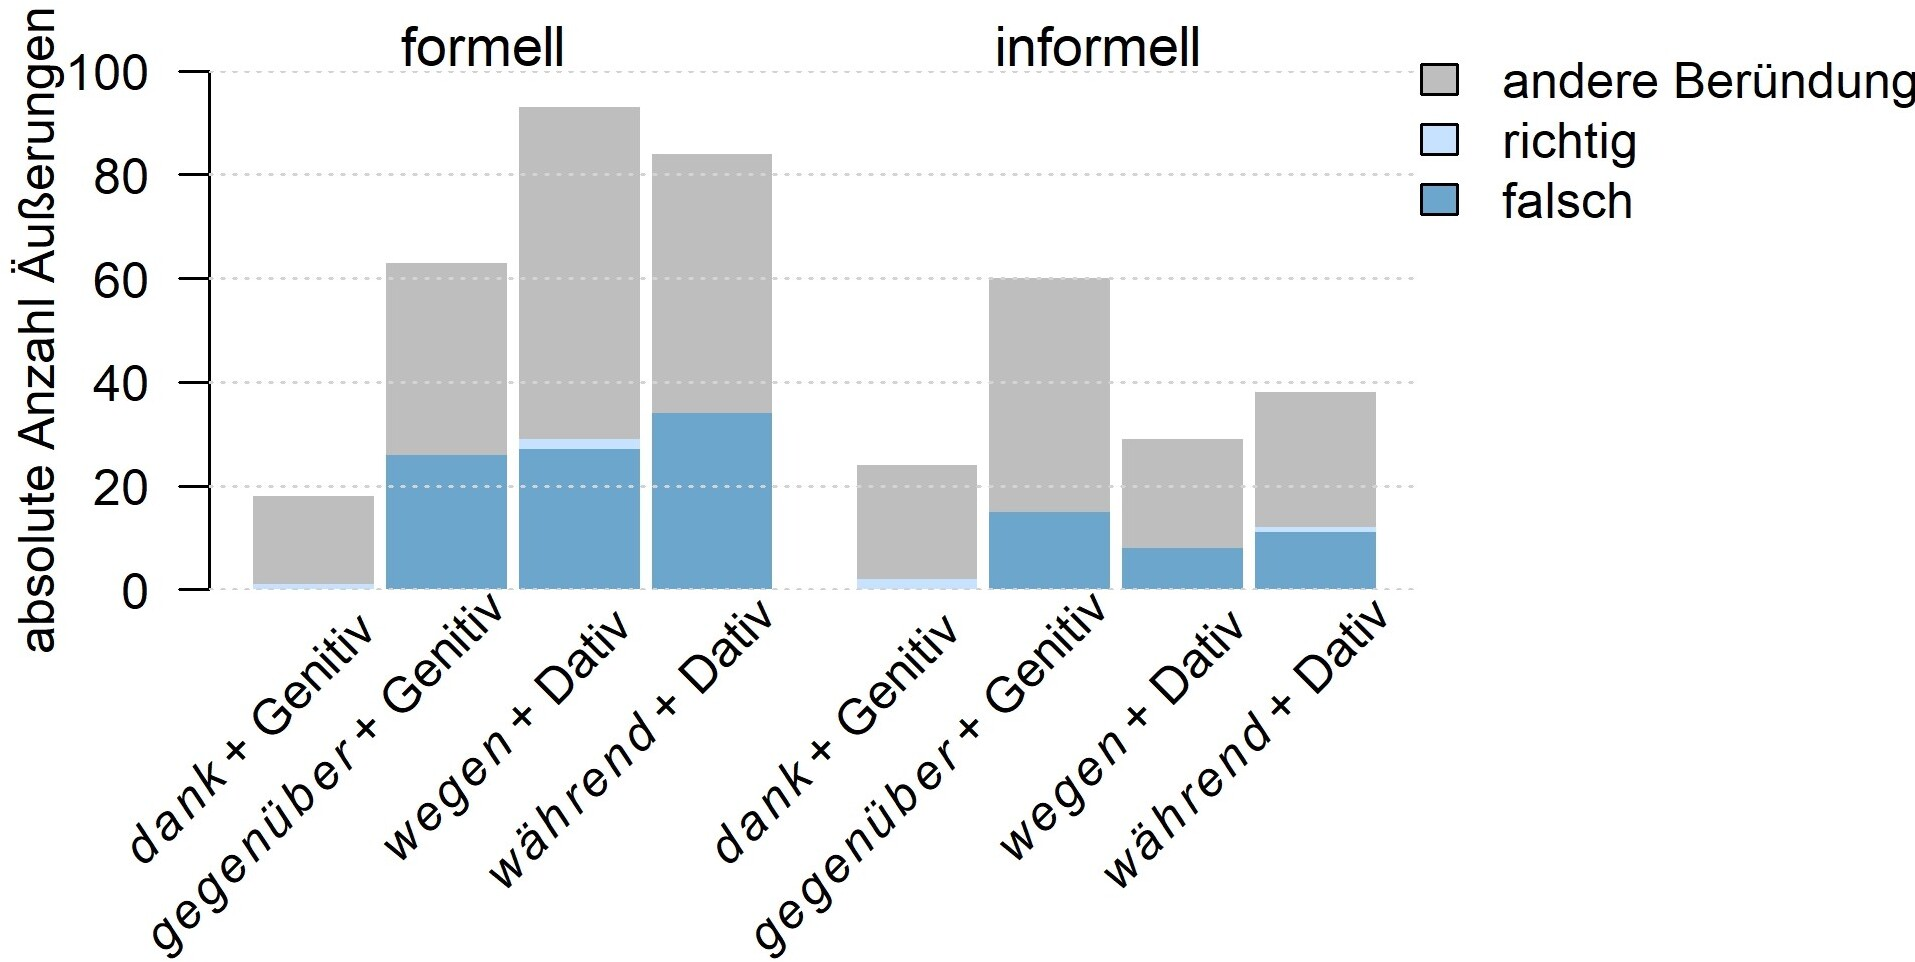
\includegraphics[width=\textwidth]{BegrKorrektheit.jpg}
\caption{Wie häufig wird die Bewertung einer Variante als unangemessen mit ihrer Inkorrektheit bzw. Korrektheit begründet?}
\label{pic:BegrKorrektheit}
\end{figure}

Im formellen Setting des Akzeptabilitätstests wird die Unangemessenheit absolut gesehen häufiger über die Inkorrektheit einer Variante erklärt als im informellen Setting, allerdings werden die Dativvarianten mit \wegen{} und \waehrend{} in diesem Setting auch insgesamt deutlich häufiger als unangemessen bewertet. 
Bei \wegen{} plus Dativ unterscheidet sich der Anteil der Begründungen, die die Inkorrektheit erwähnen, nicht zwischen den Settings und liegt jeweils bei ungefähr einem Drittel. 
Die Einstufung der Dativrektion bei \waehrend{} als unangemessen wird im formellen Teil jedoch häufiger mit Inkorrektheit begründet als im informellen (ca. 40~\% im Vergleich zu ca. 30~\%). 
Ebenso ist es bei \gegenueber{} plus Genitiv (rund 40~\% im Vergleich zu 25~\%). 
Dies könnte vermuten lassen, dass die Korrektheit dieser Formen für die Bewertung ihrer Angemessenheit in formellen Kontexten ausschlaggebender ist als in informellen, wie auch folgende Antwort nahelegt: 
\begin{exe}
\ex \object{Förmliche Briefe sollten auf korrekten Gebrauch der Grammatik achten.} (Germanistikstudent, 21, zu \gegenueber{} mit dem Genitiv im formellen Setting)
\end{exe} 
Dieser Befund lässt sich mit der engen konzeptuellen Verknüpfung von Formalität, Schriftlichkeit und Standardsprache erklären (\autoref{sec:Einheitlichkeit}). 
Ein formeller Kontext präsupponiert, dass die darin vorkommenden Varianten Teil der kodifizierten Norm sind. 
In \autoref{sec:ErgAkzallg} wurde dies bereits daran erkennbar, dass sich die Beurteilung von Korrektheit und Angemessenheit im formellen Setting nahezu deckt, während es im informellen Setting Diskrepanzen geben kann. 

Wenn \dank{} plus Genitiv als unangemessen beurteilt wird, wird dies nie damit begründet, dass diese Variante inkorrekt sei. 
Sehr häufig findet sich diese Begründungsstrategie hingegen bei \wegen{} und \waehrend{} mit dem Dativ. 
Im Gegensatz zur historisch neuen Dativrektion bei \wegen{} und \waehrend{} wird die ebenfalls historisch neue Genitivrektion bei \dank{} also bereits als korrekt angesehen. 
Dies unterstützt die in \autoref{cha:SekPraeps} diskutierte These, dass sich die neue Genitivrektion schneller durchsetzt als die neue Dativrektion \citep[s. auch][257]{Baumann2014}. 

%\subsection{Begründungen über Ästhetik}
Wird die Beurteilung einer Variante im Akzeptabilitätstest mit ästhetischen Gesichtspunkten begründet, wird die Form meist allgemein als schlecht oder unschön bezeichnet (zwölfmal).
Zehn dieser Äußerungen beziehen sich auf Dativvarianten, die anderen beiden auf die Genitivrektion bei \gegenueber. 
Letztere wird außerdem mit der Begründung abgelehnt, dass sie auffällig bzw. ungewohnt sei:
\begin{exe}
\ex \object{gegenüber dem Schaffner klingt natürlicher} (Junior Marketingmanagerin, 25, zu \gegenueber{} mit dem Genitiv im informellen Setting)
\end{exe} 
Wie bereits bei den freien Assoziationen (\autoref{sec:ErgAssAes}) zeigt sich auch bei den freien Antworten im Akzeptabilitätsteil eine klare Zuordnung der Rektionskasus zu bestimmten ästhetischen Eigenschaften. 
So wird ausschließlich die Genitivrektion mit der Begründung, gesteltzt, abgehoben oder überkorrekt zu klingen, als unangemessen eingestuft. 
Die Einbettung der im Akzeptabilitätstest präsentierten Beispiele in ein formelles und ein informelles Setting ermöglicht einen genaueren Blick auf den Zusammenhang der metapragmatischen Zuschreibungen mit dem Kontext, in dem eine Variante wahrgenommen wird. 
Wie auch im folgenden Beispiel wird die Genitivrektion nur im informellen Setting als gestelzt, abgehoben oder überkorrekt bewertet:
\begin{exe}
\ex \object{würde im Gespräch eher den Dativ verwenden, das klingt zu förmlich, zu gewollt} (Angestellte an einer Hochschule im Bereich Beratung und Information, 28, zu \dank{} mit dem Genitiv im informellen Setting) \label{Bsp:BegrForm1}
\end{exe}
Als plump oder schlampig werden hingegen fast ausschließlich Dativvarianten im formellen Setting beurteilt.\footnote{Auch \gegenueber{} plus Genitiv im informellen Setting wird einmal mit der Begründung abgelehnt, es klinge plump bzw. schlampig. } 

%\subsection{Begründungen über Formalität}
Die Antworten, die sich bei der Begründung, warum eine Variante als unangemessen eingestuft wurde, auf die Formalität beziehen, lassen sich in zwei Gruppen einteilen:
In die erste Gruppe fallen Antworten, in denen der abgefragten Rektionsvariante zugeschrieben wird, sie sei formell oder informell. 
Dazu zählt etwa die folgende Antwort zur Genitivrektion bei \dank{} im informellen Setting: 
\begin{exe}
\ex \object{hört sich zu formell an} (Medizinstudentin, 24, zu \dank{} mit dem Genitiv im informellen Setting)
\end{exe}
Die Befragte begründet ihre Ablehnung von \dank{} plus Genitiv in einem Gespräch mit einem Freund hier, indem sie die Form als formell bezeichnet. 
Die zweite Gruppe von Begründungen der Kategorie \glqq Formalität\grqq{} argumentiert hingegen damit, dass der Kontext Formalität oder Informalität erfordere:
\begin{exe}
\ex \object{umgangssprachlich evtl. tolerierbar, in förmlichen Briefen zeugt es aber von Unkenntnis} (Betriebswirt, 37, zu \wegen{} mit dem Dativ im formellen Setting)
\end{exe}
Der Dativ bei \wegen{} wird hier mit der Begründung abgelehnt, dass er in einem förmlichen Brief an ein Amt, der einen hohen Grad an Formalität erwarten lässt, einen negativen Eindruck macht.
Die der Variante zugeschriebene Wirkung (\textit{entailment}, \autoref{sec:Indexikalitaet}) wird also davon abhängig gemacht, welchen Grad an Formalität ein zuvor etablierter Kontext präsupponiert (\textit{presupposition}). 
Häufig wird in den Begründungen der Befragten sowohl auf die Formalitätsanforderungen des Kontexts als auch auf die dadurch entfaltete Wirkung der Variante Bezug genommen. 
Dies zeigt etwa das oben bereits angeführte \autoref{Bsp:BegrForm1}. 

%\subsection{Begründungen über Personentypen}
Die Begründungen der Kategorie \glqq Personentypus\grqq{} argumentieren für die Unangemessenheit einer Rektionsvariante, indem sie ihr bestimmte, meist negative Personeneigenschaften zuschreiben. 
Auffällig ist, dass die Dativrektion bei \wegen{} und \waehrend{} häufiger mit Personeneigenschaften in Verbindung gebracht wird als die Genitivrektion bei \dank{} und \gegenueber{} (20-mal zu sechsmal).
Im folgenden Beispiel etwa wird die Dativrektion bei \waehrend{} mit der Begründung abgelehnt, die Form wirke sprachlich unsicher und schlampig:
\begin{exe}
\ex \object{Die fehlende Sprachsicherheit bzw. \glqq schlampige\grqq{} Ausdrucksweise.} (Beamtin, 61, zu \waehrend{} mit dem Dativ im informellen Setting)
\end{exe}
Teilweise wird die Ablehnung der Dativrektion ganz allgemein damit begründet, sie mache einen schlechten Eindruck, wie etwa hier:
\begin{exe}
\ex \object{macht schlechten Eindruck -- Umgangssprache} (Englischlehrerin, 61, zu \wegen{} mit dem Dativ im formellen Setting)
\end{exe}
Für diese Antworten wurde im Kategoriensytem die Unterkategorie \glqq peinlich/schlechter Eindruck\grqq{} ergänzt. 
In \autoref{Bsp:BegrPersonentypus1} dagegen wird detailliert ausgeführt, wie die Verwendung von \waehrend{} plus Dativ in einem förmlichen Brief zu einem negativen Eindruck führt und welche Konsequenzen dies haben kann:
\begin{exe}
\ex \object{Unpassend; wer so schreibt, kann sich scheinbar nicht der Situation angemessen ausdrücken, kann nicht zwischen formellem und informellem Sprachgebrauch unterscheiden. Man begibt sich dadurch gegenüber dem Empfänger auf ein niedrigeres Niveau und vermittelt den Eindruck eines geringen Bildungsgrades; die Gefahr besteht, dass man dadurch weniger ernst genommen wird.} (Umweltplanungsstudent, 25, zu \waehrend{} mit dem Dativ im formellen Setting) \label{Bsp:BegrPersonentypus1}
\end{exe}
Der Gebrauch des Dativs wird hier als Mangel an Registerbewusstsein auf Seiten des/r Schreibenden gewertet: 
Da der Kontext Formalität erfordert, sollte die als formell registrierte Genitivrektion verwendet werden. 
Es wird impliziert, dass dieses Registerbewusstsein bei den EmpfängerInnen des Briefs (den MitarbeiterInnen eines Amts) vorhanden ist. 
Das fehlende Wissen um den registeradäquaten Gebrauch der Rektionsvarianten wird anschließend mit einem geringen Bildungsniveau in Verbindung gebracht. 
Schließlich wird die Vermutung geäußert, dass Personen mit niedrigeren Bildungsabschlüssen in der Interaktion mit einem Amt weniger ernst genommen werden. 

% Zusammenfassung
Die inhaltsanalytische Auswertung der freien Antworten auf die Frage \glqq was stört Sie?\grqq{} im Akzeptabilitätstest lässt sich wie folgt zusammenfassen:
Als Begründung für die Beurteilung der Dativrektion bei \wegen{} oder \waehrend{} sowie der Genitivrektion bei \gegenueber{} als unangemessen wird mit Abstand am häufigten angeführt, diese Formen seien inkorrekt. 
Des Weiteren nehmen Befragte auf die Ästhetik der Varianten Bezug, um zu begründen, warum sie sie als unangemesen eingestuft haben. 
Dabei werden die Dativvarianten meist allgemein als schlecht oder unschön bezeichnet, die Genitivrektion bei \gegenueber{} als auffällig und ungewohnt. 
In den Antworten, in denen Formalität thematisiert wird, wird zum einen damit argumentiert, dass eine Variante als formell oder informell registriert sei. 
Zum anderen wird darauf verwiesen, dass der im Akzeptabilitätstest vorgegebene Kontext einen bestimmten Formalitätsgrad erfordere. 
In den Antworten der Kategorie \glqq Personentypus\grqq{} wird den als unangemessen abgelehnten Varianten zugeschrieben, einen schlechten Eindruck zur Folge zu haben, indem VerwenderInnen der Varianten bspw. als ungebildet konzeptualisiert werden.

Der folgende Abschnitt liefert einen zusammenfassenden Überblick über alle quantitativen und qualitativen Ergebnisse des Akzeptabilitätstests. 
\subsection{Zusammenfassung der Auswertung des Akzeptabilitätstests}
\label{sec:ZsfsgAkz}
Im Akzeptabilitätsteil des Fragebogens wurden die Befragten -- aufgeteilt auf vier Gruppen -- nach ihrer Einschätzung der Korrektheit, der Angemessenheit und ihrer eigenen Verwendung von Rektionsvarianten in einem formellen und einem informellen Setting gefragt.
Abgefragt wurde die Dativrektion bei \wegen{} und \waehrend{} sowie die Genitivrektion bei \dank{}, \gegenueber{} und der Primärpräposition \object{seit}.

Von allen abgefragten Varianten wird \dank{} plus Genitiv am häufigsten als korrekt bewertet. 
In beiden Settings wird diese Form von der großen Mehrheit der Befragten akzeptiert. 
Die Dativrektion bei \wegen{} und \waehrend{} hingegen beurteilen im informellen Settings nur jeweils unter 30~\% der Befragten als korrekt, im formellen Setting sogar nur jeweils unter 20~\%. 
Obwohl \wegen{} und \waehrend{} mit der Dativrektion im \citet[915]{Duden2016} aufgeführt werden, werden diese Rektionsvarianten damit seltener als korrekt eingestuft als die in Korpora kaum belegte Genitivrektion bei \gegenueber{}. 
Auch bei \object{seit}, das als Primärpräposition laut kodifizierter Norm ausschließlich die Dativrektion zulässt, wird der Genitiv in beiden Settings von mindestens 20~\% der Befragten als korrekt angesehen. 

Als angemessen wird ebenfalls am häufigsten die Genitivrektion bei \dank{} gewertet. 
Sie gilt in beiden Settings als passend. 
Die Angemessenheit der Dativrektion bei \wegen{} oder \waehrend{} wird dagegen je nach Setting unterschiedlich bewertet:
Im formellen Setting entspricht der Anteil derer, die die Varianten als angemessen empfinden ungefähr dem Anteil derer, die sie auch als korrekt einstufen. 
Im informellen Setting jedoch erscheint die Dativrektion den Befragten deutlich häufiger angemessen als korrekt. 
Die Genitivrektion bei \gegenueber{} und \object{seit} wird jeweils ähnlich häufig als angemessen eingestuft wie sie als korrekt bewertet wird. 

Dass sie eine Variante selbst verwenden würden, geben jeweils etwas weniger Befragte an, als dass die Variante angemessen sei.
Bei \wegen{} und \waehrend{} mit dem Dativ zeigen sich auch hier Unterschiede zwischen den Settings:
In einem informellen Gespräch würde jeweils ca. die Hälfte die Dativrektion verwenden, in einem formellen Brief sind es nur jeweils unter 10~\%. 
Umgekehrt geben in Bezug auf die Genitivrektion bei \object{seit} im informellen Setting deutlich weniger Befragte an, die Variante zu verwenden als im formellen. 

Inwiefern sich die Beurteilung der Akzeptabilität in verschiedenen Befragtengruppen unterscheidet, wurde in \autoref{sec:ErgAkzNachAlter} bis \autoref{sec:ErgAkzNachVT} behandelt. 
Folgende Faktoren wurden dabei berücksichtigt:
das Alter der Befragten, ihre regionale Herkunft, ihr Bildungsstand, wie textaffin ihr Beruf ist und wie variationstolerant sie sind. 
Der Einfluss dieser Faktoren sowie der Formalität des Settings auf die Angaben zu Korrektheit, Angemessenheit und eigener Verwendung wurde anschließend mithilfe von \textit{Random Forests} statistisch überprüft. 
Dies zeigte, dass auf die Bewertung der Dativrektion bei \wegen{} oder \waehrend{} vor allem die Formalität des Settings sowie die regionale Herkunft der Befragten einen Einfluss haben. 
Bei der Beurteilung der Genitivrektion bei \dank{} und \gegenueber{} konnte keine Abhängigkeit von einem der untersuchten Faktoren festgestellt werden. 
Die Akzeptabilität der Genitivrektion mit der Primärpräposition \object{seit} scheint zu einem gewissen Grad davon abzuhängen, wie textaffin der Beruf der Befragten ist. 

Befragte, die im Akzeptabilitätstest eine Variante als unangemessen bewerteten, wurden in einer offenen Frage nach einer Begründung für diese Einschätzung gebeten. 
Die inhaltsanalytische Auswertung der Antworten macht erneut den engen Zusammenhang zwischen der Beurteilung von Korrektheit und Angemessenheit im formellen Setting deutlich:
Begründungen, die auf die Inkorrektheit der Form verwiesen, sind hier mit Abstand am häufigsten. 
Weitere Gründe, die für die Beurteilung einer Variante als unangemessen genannt werden, sind ästhetische Eigenschaften der Form sowie ihre indexikalische Verknüpfung mit negativen Personeneigenschaften und die damit verbundene Angst, einen schlechten Eindruck zu hinterlassen. 
Daneben wird für die Ablehnung als unangemessen argumentiert, indem der vom Kontext geforderte Grad an Formalität mit der Registrierung der Variante als formell oder informell abgeglichen wird. 
Der folgende Abschnitt widmet sich der Verwendung der Rektionsvarianten im Produktionsexperiment.  \section{Ergebnisse des Produktionsexperiments}
\label{sec:ErgProduktion}
Im letzten Teil des Ergebniskapitels wird das Produktionsexperiment aus dem Fragebogen ausgewertet. 
Es besteht aus zwei Lückentexten, bei denen die Befragten gebeten werden, in die Lücken nach den untersuchten Präpositionen die Form eines in Klammern angegebenen Substantivs und die Artikelform einzutragen (für eine ausführliche Beschreibung des Produktionsexperiments s. \autoref{sec:LU}):
Einer der Lückentexte ist einem klassischen Bewerbungsschreiben nachempfunden, der andere ist an eine private Textnachricht oder E-Mail angelehnt, sodass unterschiedliche Formalitätsgrade evoziert werden. 
Mit dem folgenden Beispielsatz etwa wird die Kasusrektion von \wegen{} im informellen Lückentext abgefragt:
\begin{exe}
\ex \object{Hab jetzt nochmal mit Max wegen \_\_\_\_\_\_ (Verkauf) auf dem Flohmarkt morgen telefoniert.}
\end{exe} 
Alle 397 Befragten füllten beide Lückentexte aus, sodass zu jeder Präposition in jedem Setting 397 Antworten vorhanden sind. 
Zusätzlich zu \wegen, \waehrend, \dank{} und \gegenueber{} wurde wie schon im Akzeptabilitätstest die Primärpräposition \object{seit} abgefragt. 
\autoref{table:ProdBsp} zeigt, welche Präposition mit welchen Substantiven abgefragt wurde.  
Die vollständigen Lückentexte finden sich im Fragebogen im Anhang (\autoref{Anh:Fragebogen}).
\begin{table}
\centering
\begin{tabular}{lcc}
\textit{\textbf{}} & formeller Lückentext & informeller Lückentext \\ \hline
\textit{wegen}     & \textit{Anspruch}             & \textit{Verkauf}                \\ %\hline
\textit{während}   & \textit{Studium}              & \textit{Aufbau}                 \\ %\hline
\textit{dank}      & \textit{Praktikum}            & \textit{Wetter}                 \\ %\hline
\textit{gegenüber} & \textit{Beruf}                & \textit{Plan}                   \\ %\hline
\textit{seit}      & \textit{Wegfall}              & \textit{Streit}                 \\ 
\end{tabular}
\caption{Übersicht über die Substantive, mit denen die Präpositionen im Produktionsexperiment abgefragt wurden}
\label{table:ProdBsp}
\end{table}

Im Folgenden wird überprüft, inwiefern sich die Indexikalität der Dativ- und der Genitivrektion in der Verwendung der beiden Varianten widerspiegelt. 
Die Auswertung der freien Assoziationen sowie auch die Ergebnisse des Akzeptabilitätstest haben gezeigt, dass die Rektionsvarianten metapragmatisch mit Kategorien wie (In)Korrektheit, (In)Formalität, Standardsprache, Regionalsprache, Sprachwandel und mit verschiedenen Personentypen verknüpft sind. 
Wie diese mit der Kasuswahl in den Lückentexten zusammenhängen, wird im Folgenden näher beleuchtet. 

% Änderung Anfang!
Um sicherzugehen, dass die als unterschiedlich formell konzipierten Lückentext von Befragten auch so eingeschätzt werden, wurde die Wahrnehmung der Formalität beider Texte in einer zusätzlichen Umfrage überprüft. 
Auf diese Überprüfung wird in \autoref{sec:FormLU} eingegangen. 
% Änderung Ende!
Sowohl die Auswertung der freien Assoziationen als auch die Ergebnisse des Akzeptabilitätstests unterstreichen, wie relevant die Formalität des Kontexts ist. Daher wird in \autoref{sec:ErgProdInfForm} die Kasuswahl im formellen Lückentext mit der Kasuswahl im informellen Lückentext verglichen. 
Anschließend werden unterschiedliche Befragtengruppen in den Blick genommen, die indexikalisch mit einem bestimmten Kasusgebrauch verknüpft sind:
In \autoref{sec:ErgProdNachAlter} wird untersucht, wie das Alter der Befragten mit ihrer Kasuswahl zusammenhängt.
Dies ist relevant, da die Kategorie \glqq Alter\grqq{} über die Konzeptualisierung als Sprachwandelphänomen mit der Rektionsvariation indexikalisch verknüpft ist. 
Da die Rektionsvarianten sich in ihrer Verortung in Regional- und Standardsprache unterscheiden, wird in \autoref{sec:ErgProdNachHerkunft} die Kasuswahl nord- und süddeutscher Befragter verglichen. 
\autoref{sec:ErgProdNachBildung} und \autoref{sec:ErgProdNachSk} nehmen einen Vergleich der Kasuswahl nach dem Bildungsstand der Befragten und nach der Textaffinität ihres Berufs vor und richten den Blick damit auf die {Ka\-te\-gorien} \glqq Bildung\grqq{} und \glqq Sprachkompetenz\grqq.
Schließlich geht es in \autoref{sec:ErgProdNachVT} um die Abhängigkeit der Kasuswahl von der Variationstoleranz, die als Indikator dafür gewertet werden kann, wie stark sich Befragte der Standardsprachideologie verschreiben. 

Der Einfluss der in \autoref{sec:ErgProdInfForm} bis \autoref{sec:ErgProdNachVT} dargestellten Faktoren auf die Kasuswahl bei \wegen, \waehrend, \dank, \gegenueber{} und der Primärpräposition \object{seit} wird mithilfe von \textit{Conditional Inference Trees} und \textit{Random Forests} statistisch überprüft (\autoref{sec:ErgProdCTrees}). 
\autoref{sec:ErgProdZusammenfassung} bietet eine Zusammenfassung der Ergebnisse aus dem Produktionsexperiment. 
%Änderung Anfang!
\subsection{Wahrgenommene Formalität der Lückentexte}
\label{sec:FormLU}
In einer zusätzlichen Umfrage wurde überprüft, inwiefern die beiden Lückentexte von SprachbenutzerInnen als unterschiedlich formell wahrgenommen werden. 
Hierfür wurden die Texte nicht als Lückentexte präsentiert, sondern die Präpositionen \textit{wegen}, \textit{während}, \textit{dank}, \textit{gegenüber} und \textit{seit} erschienen entweder alle mit dem Genitiv oder alle mit dem Dativ. 
Insgesamt wurden 63 Personen\footnote{Das Durchschnittsalter liegt bei 35 Jahren, 45 Personen sind weiblich, 16 männlich, eine Person ordnet sich einem anderen Geschlecht zu und eine Person möchte keine Angabe zu ihrem Geschlecht machen. Regional sind die Befragten über ganz Deutschland verteilt.} über SoSciSurvey \citep{Leiner.2014} befragt.
Sie wurden per Zufallsgenerator auf vier Gruppen aufgeteilt: 
\begin{enumerate}
\item Formell gestalteter Lückentext (Bewerbungsschreiben) mit Dativrektion bei allen Präpositionen
\item Formell gestalteter Lückentext (Bewerbungsschreiben) mit Genitivrektion bei allen Präpositionen 
\item Informell gestalteter Lückentext (private Textnachricht) mit Dativrektion bei allen Präpositionen
\item Informell gestalteter Lückentext (private Textnachricht) mit Genitivrektion bei allen Präpositionen
\end{enumerate}
\autoref{pic:WahrnFormLu} zeigt, wie formell die einzelnen Texte von den Befragten wahrgenommen werden. 
\begin{figure}
\centering
\includegraphics[width=\textwidth]{WahrnFormLu}
\caption{Wahrnehmung der Formalität der Lückentexte}
\label{pic:WahrnFormLu}
\end{figure}

Der einem Bewerbungsschreiben nachempfundene Text mit Dativrektion bei allen Präpositionen wird von fünf Befragten als formell und von sechs Befragten als eher formell eingestuft.\footnote{Im Fragebogen waren die Zwischenstufen bewusst nicht beschriftet. Bezeichnungen wie \glqq eher formell\grqq{} werden hier lediglich genutzt, um die einzelnen Stufen zu benennen.} 
Zwei Personen wählten den mittleren Skalenpunkt, konnten sich also nicht zwischen formell und informell entscheiden. Eine Person gibt an, den Text als eher informell wahrzunehmen. 
Wird Befragten der gleiche Text mit der Genitivrektion bei allen Präpositionen vorgelegt, sieht die Verteilung ähnlich aus. 
Hier entscheiden sich insgesamt 15 Personen für formell bzw. eher formell, eine Person empfindet den Text als eher informell. 

Der zweite Text, der durch Mündlichkeits- und Informalitätsmarker an eine private Textnachricht erinnern soll, wird von dern Befragten als deutlich informeller wahrgenommen. 
Bei der Version mit Dativrektion geben 13 Personen an, den Text als informell wahrzunehmen, fünf Befragte geben durch Auswahl der angrenzenden Skalenstufe an, dass sie den Text als eher formell wahrnehmen. 
Eine Person entscheidet sich für die mittlere Skalenstufe und eine weitere Person nimmt den Text als eher formell wahr. 
Der gleiche Text mit Genitivrektion wird von acht Befragten als informell und von vier als eher informell empfunden.
Eine Person wählt die mittlere Skalenstufe. 

Insgesamt zeigt die Überprüfung der wahrgenommenen Formalität der Texte, dass diese jeweils geeignet sind, um als Lückentexte unterschiedliche Formalitätsgrade zu evozieren. 
 
% Änderung Ende! 

\subsection{Kasuswahl im formellen und im informellen Lückentext}
\label{sec:ErgProdInfForm}
% Kasuswahl nach Register
Für die Auswertung der Lückentexte wurden alle Textfeldeingaben, die eindeutig als Genitivform erkennbar sind, zusammengefasst (etwa \object{des Plans} und \object{des Planes}) sowie alle Eingaben, die eindeutig als Dativform erkennbar sind (etwa \object{dem Plan} und \object{Dem Plan}).\footnote{Dem Genitiv wurde auch die Pluralform \object{der Verkäufe} zugerechnet.} 
Neben den als Dativ oder Genitiv klassifizierten Antworten gibt es außerdem Antworten, die keinem der beiden Kasus zugeordnet werden konnten (etwa \object{dem Verkaufs}). 
Diese wurden in der Kategorie \glqq Sonstiges\grqq{} zusammengefasst. 
Im Folgenden wird zunächst die Kasuswahl bei den Sekundärpräpositionen besprochen, anschließend die Wahl bei der Primärpräposition \object{seit}.

\autoref{pic:KasuswahlNachRegister} zeigt für alle vier Sekundärpräpositionen, wie häufig prozentual Genitiv- und Dativformen sowie sonstige Formen im formellen und im informellen Lückentext gewählt wurden. 
Das augenfälligste Ergebnis ist, dass die Genitivrektion bei allen Präpositionen bis auf \gegenueber{} insgesamt deutlich überwiegt.
Sowohl bei den ursprünglichen Genitivpräpositionen \wegen{} und \waehrend{} als auch bei der ursprünglichen Dativpräposition \dank{} wurde der Genitiv im formellen und im informellen Lückentext häufiger gewählt als der Dativ (für die genauen Zahlen s. auch \autoref{table:AnhProd} im Anhang). 
Bei \wegen{} und \waehrend{} im informellen Text ist dieses Ergebnis vor dem Hintergrund der Angaben im Akzeptabilitätstest zunächst überraschend: 
Die Mehrheit der Befragten empfindet die Dativrektion bei diesen Präpositionen in einem informellen Gespräch als angemessen und ungefähr die Hälfte gibt an, den Dativ selbst zu verwenden (\autoref{sec:ErgAkzallg}). 
Für die Verwendung scheint jedoch eher die Einschätzung als korrekt enscheidend zu sein: 
Der Anteil der Dativrektion im Produktionsexperiment entspricht ungefähr dem Anteil der Bewertung dieser Variante als korrekt. 
Bei \gegenueber{} verwenden dagegen die allermeisten Befragten in beiden Lückentexten die Dativrektion (jeweils knapp 90~\%).
Hier ist der Anteil derer, die den Genitiv setzen, also deutlich geringer als der Anteil derer, die diesen Kasus im Akzeptabilitätstest als korrekt oder angemessen bewerten (\autoref{sec:ErgAkzallg}). 
\begin{figure}
\centering
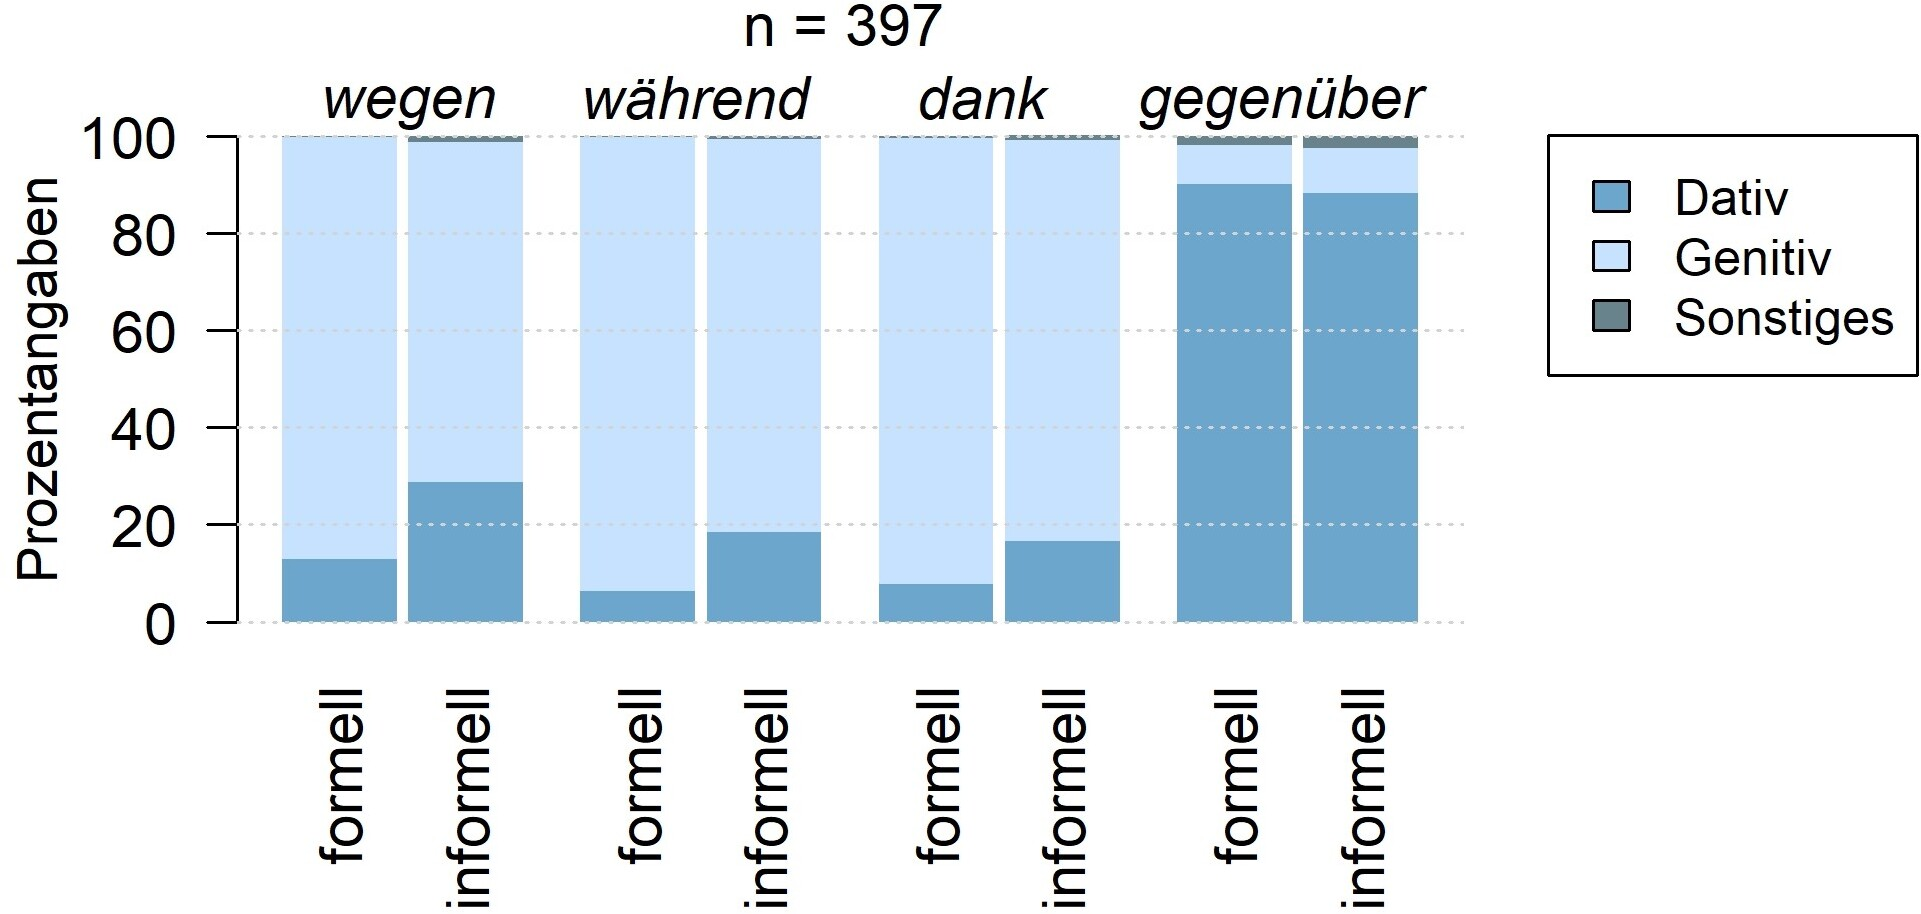
\includegraphics[width=\textwidth]{KasuswahlNachRegister}
\caption{Ergebnisse des Produktionsexperiments}
\label{pic:KasuswahlNachRegister}
\end{figure}

Obwohl insgesamt der Genitiv also klar bevorzugt wird, ist in den Daten ein deutlicher Unterschied zwischen dem formellen und dem informellen Lückentext erkennbar.
Die Dativrektion ist im informellen Teil des Produktionsexperiments weitaus häufiger.
Bei \wegen{} wählen im formellen Teil rund 87~\% der Befragten den Genitiv, im informellen Teil hingegen nur ca. 70~\%. 
\object{Während} wird im formellen Lückentext von ungefähr 94~\% mit dem Genitiv verwendet, im informellen Lückentext jedoch nur von ungefähr 81~\%. 
Bei \dank{} entscheiden sich ca. 92~\% im formellen Teil für den Genitiv und rund 82~\% im informellen Teil. 
Lediglich bei \gegenueber{} ist kein nennenswerter Unterschied erkennbar (ca. 8~\% Genitivrektion im formellen Lückentext und ca. 9~\% im informellen). 

Dass die Genitivrektion bei \wegen, \waehrend{} und \dank{} insgesamt so stark überwiegt, kann auf die Wirkung der Indexikalität zurückgeführt werden: 
Indem sie im Produktionsexperiment die Genitivrektion nutzen, inszenieren sich Befragte als gebildet, professionell und kompetent. 
Damit positionieren sie sich gegenüber der Forscherin und der Institution, der sie angehört. 
Dabei spielte wahrscheinlich auch eine Rolle, dass die Befragung von einigen als Testsituation empfunden wurde, wie Kommentare von Befragten deutlich machen:  
\begin{exe}
\ex \object{gibt es ein Lösungsblatt? Je mehr man darüber nachdenkt, desto unsicherer wird man...} (Sonderpädagogikstudent, 24) \label{Bsp:Loesungsblatt}
\ex \object{Auflösung der Textbeispiele wäre noch interessant gewesen} (keine Berufsangabe, männlich, 37) \label{Bsp:Aufloesung}
\ex \object{Im Test war ich bei der Aufgabe mit der Bewerbung teilweise mit dem englischen Fachjargon überfordert, bzw. ich kannte dort einige Begriffe nicht.} (keine Berufsangabe, weiblich, 32) \label{Bsp:Test}
\end{exe}
In einer solchen Testsituation könnte der Genitiv angemessener erscheinen, da er als standardsprachlich und daher korrekt gilt (s. Ergebnisse in \autoref{sec:ErgAssKorrektheit} und \autoref{sec:ErgAssFormMedVar}). 
Der Befragte, von dem der Kommentar in \autoref{Bsp:Loesungsblatt} stammt, verwendet im Produktionsexperiment immer den Genitiv, außer im Fall von \object{seit} im formellen Lückentext. 
Bei den Befragten, von denen die beiden anderen Kommentare stammen, lässt sich eine solch starke Tendenz zum Genitiv jedoch nicht erkennen.\footnote{Der Befragte aus \autoref{Bsp:Aufloesung} verwendet in beiden Lückentexten bei \wegen{}, \waehrend{} und \dank{} den Genitiv, bei \gegenueber{} und \object{seit} den Dativ. Die Befragte aus \autoref{Bsp:Test} verwendet im formellen Teil ebenfalls \wegen{}, \waehrend{} und \dank{} mit dem Genitiv, im informellen jedoch nur \wegen{} und \waehrend{}.}

Berücksichtigt man, dass die Befragten sich einer Sprachautorität gegenübersehen, die scheinbar ihr sprachliches Können testet, sind die Unterschiede zwischen dem formellen und dem informellen Lückentext umso bemerkenswerter. 
Es ist zu vermuten, dass der Genitiv in natürlichen informellen Interaktionssituationen seltener gebraucht wird und Formalität und Kasuswahl daher im natürlichen Sprachgebrauch noch sehr viel stärker interagieren. 
%GLMM berichten 
%Diese Ergebnisse deuten darauf hin, dass die Verweiskraft der Varianten einen Einfluss auf die Verwendung hat: Der Dativ gilt eher in informellen Kontexten als angemessen, Genitiv in formellen.
% korreliert häufiger Genitivgebrauch im formellen Setting mit häufigem Genitivgebrauch im informellen Setting?

\autoref{pic:KasuswahlSeit} zeigt die Kasuswahl bei der Primärpräposition \object{seit} im Produktionsexperiment. 
Wie bei Primärpräpositionen zu erwarten, überwiegt die Dativrektion deutlich. 
Allerdings entscheiden sich im formellen Lückentext immerhin ca. 11~\% der Befragten für die Genitivrektion (s. auch \autoref{table:AnhProd} im Anhang). 
\object{Seit} wird im formellen Teil also sogar etwas häufiger mit dem Genitiv verwendet als \gegenueber. 
Im informellen Teil wählen nur ca. 6~\% den Genitiv mit \object{seit}. 
Auch bei der Primärpräposition, die eigentlich keine Kasusschwankung aufweist, ist also trotz des insgesamt eher formellen Settings der Befragung ein Zusammenhang zwischen der Kasuswahl der Befragten und dem Register erkennbar. 
In beiden Settings ist die Zahl der Befragten, die die Genitivrektion bei \object{seit} verwenden, niedriger als die Zahl derer, die sie im Akzeptabilitätstest als korrekt oder angemessen bewerten (\autoref{sec:ErgAkzallg}). 
\begin{figure}
\centering
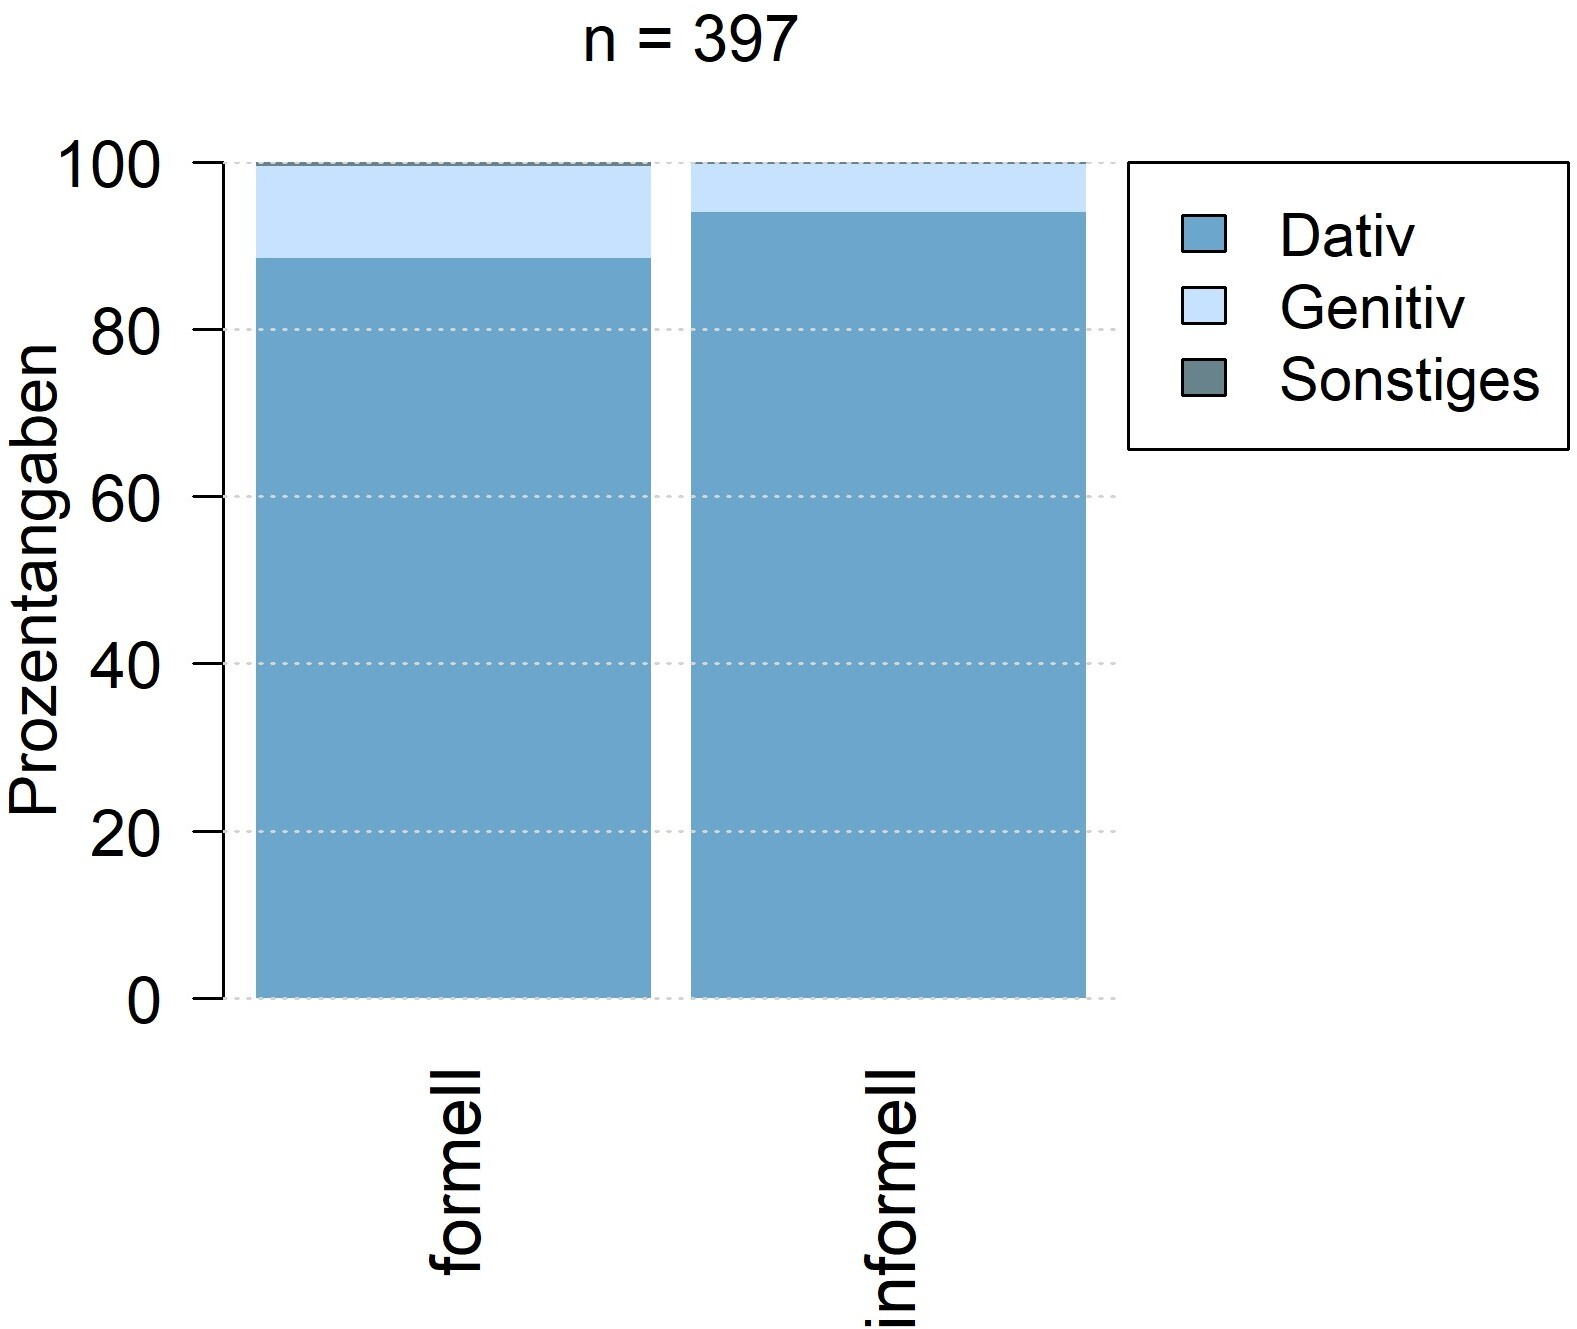
\includegraphics[width=\textwidth]{KasuswahlNachRegisterSeit.jpg}
\caption{Kasuswahl im Produktionsexperiment bei der Primärpräposition \object{seit}}
\label{pic:KasuswahlSeit}
\end{figure}

Wie in \autoref{sec:ErgAkzallg} erwähnt, könnte die Möglichkeit der kausalen Interpretation von \object{seit} die Wahl des Genitivs begünstigen. 
Im formellen Lückentext lautet der Satz, mit dem die Rektion von \object{seit} abgefragt wird, \object{seit \_\_\_\_\_ (Wegfall) einer Stelle war ich sogar für die Organisation eines Weiterbildungsworkshops zuständig}.
Der Satz im informellen Lückentext ist \object{seit \_\_\_\_\_ (Streit) neulich hab ich nix mehr von ihm gehört}.
Beide Sätze lassen neben einer temporalen auch eine kausale Lesart zu, da diese beiden Konzepte metonymisch miteinander verknüpft sind \citep[s.][]{Traugott.1991}. 
%Im Falle des ersten kann sogar davon ausgegangen werden, dass diese Lesart dominiert: 
%Die Präpositionalphrase liefert hier die Erklärung dafür, warum die Verfasserin des Bewerbungsschreibens als Werkstudentin eine so verantwortungsvolle Aufgabe wie die Organisation eines Weiterbildungsworkshops innehatte.
%Im Falle des Satzes aus dem informellen Lückentext sind die temporale und die kausale Lesart gleichermaßen plausibel, da hier die Möglichkeit offengehalten wird, dass der erwähnte Freund sich aus einem anderen Grund nicht gemeldet hat. 
%Der häufigere Gebrauch der Genitivrektion mit \object{seit} im formellen Lückentext könnte also auch in der stärker kausalen Lesart der Präpositionalphrase begründet sein. 

An den Ergebnissen des Produktionsexperiments wird deutlich, dass der Grad der Formalität, der in einem Kontext bereits etabliert ist, einen Einfluss auf die Wahl der Rektionsvariante bei \wegen{}, \waehrend{} und \dank{} hat: 
Die Dativrektion gilt eher in informellen Kontexten als angemessen, die Genitivrektion in formellen. 
Diese Registerunterschiede zeigen sich trotz einer generellen 
Tendenz zum Genitiv, die sich wahrscheinlich mit der Befragungssituation erklären lässt, in der sich Befragte als gebildet und sprachkompetent positionieren möchten.
In den folgenden Abschnitten wird untersucht, welche weiteren Faktoren eine Rolle bei der Kasuswahl spielen. 
\subsection{Kasuswahl und Alter}
\label{sec:ErgProdNachAlter}
Wie bereits für die Akzeptabilität (\autoref{sec:ErgAkzNachAlter}) soll auch für die Produktion untersucht werden, ob die älteste Befragtengruppe (61--85 Jahre) sich von der jüngsten Befragtengruppe (18--25) unterscheidet. 
Die Kategorie \glqq Alter\grqq{} ist deswegen von Interesse, weil die Rektionsschwankung der Sekundärpräpositionen als Sprachwandelphänomen konzeptualisiert wird: 
Wie in \autoref{sec:ErgAssSprachwandel} beschrieben, gehen Befragte dabei meist davon aus, dass die Genitivrektion die ältere Variante sei.
In den freien Assoziationen werden die Beispiele zwar nur selten explizit älteren Personen zugeschrieben (\autoref{sec:ErgAssPersonen}), allerdings werden sie mit Eigenschaften in Verbindung gebracht, die in der Gesellschaft häufig als typisch für ältere Menschen gelten. 
So nennen Befragte die Genitivvarianten im Fragebogen etwa streng, seriös und altmodisch.  
Der sozialsymbolische Verweis auf die Kategorie \glqq Alter\grqq{} ist also nicht auf der ersten, sondern auf der zweiten oder dritten indexikalischen Ordnung angesiedelt (\autoref{sec:Indexikalitaet}). 

Um zu überprüfen, ob sich verschiedene Altersguppen in ihrem Gebrauch der Genitiv- und Dativrektion tatsächlich unterscheiden, wird die Kasuswahl der 18- bis 25-Jährigen im Produktionsexperiment mit derjenigen der 61- bis 85-Jährigen verglichen. 
Anders als bei den Ergebnissen des Akzeptabilitätsteils werden die vier Sekundärpräpositionen \wegen, \waehrend, \dank{} und \gegenueber{} sowie die Primärpräposition \object{seit} hier einzeln betrachtet, da im Produktionsexperiment alle 397 Befragten alle Lücken bearbeiteten. 
Die Altersgruppe 18 bis 25 umfasst 104 Befragte, die Altersgruppe 61 bis 85 nur 47. 
Beim Vergleich der beiden Gruppen ist zu berücksichtigen, dass unter den älteren Befragten besonders viele Personen aus Norddeutschland sowie besonders viele Personen ohne Abitur sind (\autoref{sec:HerkunftundDialekt} und \autoref{sec:Bildung}). 
Aufgrund der geringen Anzahl der Befragten in der höheren Altersgruppe dienen die Prozentangaben im Folgenden lediglich zur besseren Orientierung beim Vergleich zwischen den Gruppen und sind allein nicht aussagekräftig. 

\autoref{table:ErgProdWegenNachAlter} zeigt die Kasuswahl bei \wegen{} in der Gruppe der 18- bis 25-Jährigen sowie in der Gruppe der 61- bis 85-Jährigen.
Im formellen Lückentext wird \wegen{} von den jüngeren Befragten kaum anders verwendet als von den älteren Befragten. 
Von den jüngeren BefragungsteilnehmerInnen entscheiden sich hier rund 10~\% für den Dativ, von den älteren ca. 11~\% (fünf Personen). 
Leichte Unterschiede zwischen den Gruppen zeigen sich im informellen Teil des Produktionsexperiments:
Hier setzen ca. 29~\% der 18- bis 25-Jährigen den Dativ, aber nur ungefähr 23~\% (elf Personen) der 61- bis 85-Jährigen. 
Die Jüngeren scheinen ihre Kasuswahl also etwas stärker von der Formalität des Settings abhängig zu machen. 
% Please add the following required packages to your document preamble:
% \usepackage{multirow}
\begin{table}
\centering
\begin{tabular}{llrr|rr}
\multicolumn{6}{l}{\textit{\textbf{wegen}}}                                                                                                                                                                                                                     \\ \hline
                                                                                  &           & \multicolumn{2}{c}{\begin{tabular}[c]{@{}c@{}}\textbf{18--25 Jahre}\\ (n=104)\end{tabular}} & \multicolumn{2}{|c}{\begin{tabular}[c]{@{}c@{}}\textbf{61--85 Jahre}\\ (n=47)\end{tabular}} \\ \hline
\multirow{3}{*}{\begin{tabular}[c]{@{}l@{}}formeller \\ Lückentext\end{tabular}}  & Dativ     & 10                                  & (9,62 \%)                                  & 5                                   & (10,64 \%)                                 \\ %\cline{2-6} 
                                                                                  & Genitiv   & 94                                  & (90,38 \%)                                 & 41                                  & (87,23 \%)                                 \\ %\cline{2-6} 
                                                                                  & Sonstiges  & 0                                   & (0 \%)                                     & 1                                   & (2,13 \%)                                  \\ \hline
\textbf{}                                                                         & \textbf{} & \multicolumn{2}{c}{\begin{tabular}[c]{@{}c@{}}\textbf{18--25 Jahre}\\ (n=104)\end{tabular}} & \multicolumn{2}{|c}{\begin{tabular}[c]{@{}c@{}}\textbf{61--85 Jahre}\\ (n=47)\end{tabular}} \\ \hline
\multirow{3}{*}{\begin{tabular}[c]{@{}l@{}}informeller\\ Lückentext\end{tabular}} & Dativ     & 30                                  & (28,85 \%)                                 & 11                                  & (23,4 \%)                                  \\ %\cline{2-6} 
                                                                                  & Genitiv   & 72                                  & (69,23 \%)                                 & 35                                  & (74,47 \%)                                 \\ %\cline{2-6} 
                                                                                  & Sonstiges  & 2                                   & (1,92 \%)                                  & 1                                   & (2,13 \%)                                  \\ \hline
\end{tabular}
\caption{Kasuswahl bei \wegen{} im formellen und im informellen Lückentext nach Altersgruppen}
\label{table:ErgProdWegenNachAlter}
\end{table}

Auch bei der Präposition \waehrend{} verhalten sich jüngere und ältere Befragte im formellen Lückentext untereinander sehr ähnlich (s. \autoref{table:ErgProdWaehrendNachAlter}). 
Nur ca. 5 bzw. 4~\% setzen den Dativ.
Im informellen Teil zeigen sich bei \waehrend{} aber deutliche Unterschiede:
Ungefähr 22~\% der 18- bis 25-Jährigen entscheiden sich hier für die Dativrektion, unter den 61- bis 85-Jährigen sind es jedoch gerade einmal ca. 2~\%, was bei der geringen Gruppengröße einer einzigen Person entspricht. 
Die Unterschiede zwischen den Altersgruppen im informellen Lückentext sind bei \waehrend{} also größer als bei \wegen, d.\,h., die Kontextsensitivität der Jüngeren zeigt sich hier noch stärker. 
% Please add the following required packages to your document preamble:
% \usepackage{multirow}
% \usepackage[table,xcdraw]{xcolor}
% If you use beamer only pass "xcolor=table" option, i.e. \documentclass[xcolor=table]{beamer}
\begin{table}
\centering
\begin{tabular}{llrr|rr}
\multicolumn{6}{l}{\textit{\textbf{während}}}                                                                                                                                                                                                                         \\ \hline
                                                                                   &           & \multicolumn{2}{c}{\begin{tabular}[c]{@{}c@{}}\textbf{18--25 Jahre}\\ (n=104)\end{tabular}} & \multicolumn{2}{|c}{\begin{tabular}[c]{@{}c@{}}\textbf{61--85 Jahre}\\ (n=47)\end{tabular}} \\ \hline
                                                                                   & Dativ     & {\color[HTML]{000000} 5}             & {\color[HTML]{000000} (4,81 \%)}             & {\color[HTML]{000000} 2}             & {\color[HTML]{000000} (4,26 \%)}            \\ %\cline{2-6} 
                                                                                   & Genitiv   & {\color[HTML]{000000} 99}            & {\color[HTML]{000000} (95,19 \%)}            & {\color[HTML]{000000} 44}            & {\color[HTML]{000000} (93,62 \%)}           \\ %\cline{2-6} 
\multirow{-3}{*}{\begin{tabular}[c]{@{}l@{}}formeller \\ Lückentext\end{tabular}}  & Sonstiges  & {\color[HTML]{000000} 0}             & {\color[HTML]{000000} (0 \%)}                & {\color[HTML]{000000} 1}             & {\color[HTML]{000000} (2,13 \%)}            \\ \hline
\textbf{}                                                                          & \textbf{} & \multicolumn{2}{c}{\begin{tabular}[c]{@{}c@{}}\textbf{18--25 Jahre}\\ (n=104)\end{tabular}} & \multicolumn{2}{|c}{\begin{tabular}[c]{@{}c@{}}\textbf{61--85 Jahre}\\ (n=47)\end{tabular}} \\ \hline
                                                                                   & Dativ     & {\color[HTML]{000000} 23}            & {\color[HTML]{000000} (22,12 \%)}            & {\color[HTML]{000000} 1}             & {\color[HTML]{000000} (2,13 \%)}            \\ %\cline{2-6} 
                                                                                   & Genitiv   & {\color[HTML]{000000} 81}            & {\color[HTML]{000000} (77,88 \%)}            & {\color[HTML]{000000} 45}            & {\color[HTML]{000000} (95,74 \%)}           \\ %\cline{2-6} 
\multirow{-3}{*}{\begin{tabular}[c]{@{}l@{}}informeller\\ Lückentext\end{tabular}} & Sonstiges  & {\color[HTML]{000000} 0}             & {\color[HTML]{000000} (0 \%)}                & {\color[HTML]{000000} 1}             & {\color[HTML]{000000} (2,13 \%)}            \\ \hline
\end{tabular}
\caption{Kasuswahl bei \waehrend{} im formellen und im informellen Lückentext nach Altersgruppen}
\label{table:ErgProdWaehrendNachAlter}
\end{table}

Wie bereits bei den beiden ursprünglichen Genitivpräpositionen \wegen{} und \waehrend{} gibt es auch bei der ursprünglichen Dativpräposition \dank{} im formellen Teil des Produktionsexperiments kaum Unterschiede zwischen den beiden Altersgruppen (s. \autoref{table:ErgProdDankNachAlter}). 
% Please add the following required packages to your document preamble:
% \usepackage{multirow}
\begin{table}
\centering
\begin{tabular}{llrr|rr}
\multicolumn{6}{l}{\textit{\textbf{dank}}}                                                                                                                                                                                                                           \\ \hline
                                                                                  &           & \multicolumn{2}{c}{\begin{tabular}[c]{@{}c@{}}\textbf{18--25 Jahre}\\ (n=104)\end{tabular}} & \multicolumn{2}{|c}{\begin{tabular}[c]{@{}c@{}}\textbf{61--85 Jahre}\\ (n=47)\end{tabular}} \\ \hline
\multirow{3}{*}{\begin{tabular}[c]{@{}l@{}}formeller \\ Lückentext\end{tabular}}  & Dativ     & 7                                    & (6,73 \%)                                    & 4                                    & (8,51 \%)                                   \\ %\cline{2-6} 
                                                                                  & Genitiv   & 97                                   & (93,27 \%)                                   & 43                                   & (91,49 \%)                                  \\ %\cline{2-6} 
                                                                                  & Sonstiges  & 0                                    & (0 \%)                                       & 0                                    & (0 \%)                                      \\ \hline
\textbf{}                                                                         & \textbf{} & \multicolumn{2}{c}{\begin{tabular}[c]{@{}c@{}}18--25 Jahre\\ (n=104)\end{tabular}} & \multicolumn{2}{|c}{\begin{tabular}[c]{@{}c@{}}61--85 Jahre\\ (n=47)\end{tabular}} \\ \hline
\multirow{3}{*}{\begin{tabular}[c]{@{}l@{}}informeller\\ Lückentext\end{tabular}} & Dativ     & 22                                   & (21,15 \%)                                   & 6                                    & (12,77 \%)                                  \\ %\cline{2-6} 
                                                                                  & Genitiv   & 81                                   & (77,88 \%)                                   & 40                                   & (85,11 \%)                                  \\ %\cline{2-6} 
                                                                                  & Sonstiges  & 1                                    & (0,96 \%)                                    & 1                                    & (2,13 \%)                                   \\ \hline
\end{tabular}
\caption{Kasuswahl bei \dank{} im formellen und im informellen Lückentext nach Altersgruppen}
\label{table:ErgProdDankNachAlter}
\end{table}

In beiden Gruppen wählen die allermeisten Befragten die Genitivrektion (ca. 93 bzw. 91,5~\%). 
Im informellen Lückentext tendieren jüngere Befragte auch bei \dank{} stärker zur Dativrektion als ältere Befragte. 
Während sich von den unter 26-Jährigen ca. 21~\% für die Dativrektion entscheiden, sind es bei den über 60-Jährigen nur ca. 13~\% (sechs Personen). 
Entscheidend ist also nicht, welche Rektionsvariante älter ist, sondern welcher Rektionsvariante metapragmatisch zugeschrieben wird, die ältere zu sein: 
Obwohl es sich bei \dank{} plus Dativ um die ältere Variante handelt, wird diese von der älteren Befragtengruppe nicht häufiger verwendet. 
Dies verdeutlicht, dass es eine zu starke Vereinfachung darstellt, das Alter der Befragten als bloßen Indikator für Sprachwandel heranzuziehen, wie es in soziolinguistischen Studien häufig üblich war und teilweise immer noch ist (\autoref{sec:WandeldurchIndexikalitaet}). 

Anders als bei \wegen, \waehrend{} und \dank{} zeigen sich bei der noch kaum schwankenden Präposition \gegenueber{} Unterschiede zwischen den Altersgruppen lediglich im formellen, nicht aber im informellen Lückentext (s. \autoref{table:ErgProdGegenueberNachAlter}). 
In dem Teil des Produktionsexperiments, der an ein klassisches Bewerbungsschreiben angelehnt ist, setzen unter den 18- bis 25-Jährigen etwas mehr den Genitiv (ca. 11~\%) als unter den 61- bis 85-Jährigen (ca. 4~\% bzw. zwei Personen). 
Im informellen Lückentext setzen jeweils ungefähr 89~\% den Dativ. 
Damit zeigt sich bei den Jüngeren ein Zusammenhang von Kasuswahl und Kontextformalität: Im formellen Lückentext wird der Genitiv etwas häufiger gesetzt. 
% Please add the following required packages to your document preamble:
% \usepackage{multirow}
\begin{table}
\centering
\begin{tabular}{llrr|rr}
\multicolumn{6}{l}{\textit{\textbf{gegenüber}}}                                                                                                                                                                                                                      \\ \hline
                                                                                  &           & \multicolumn{2}{c}{\begin{tabular}[c]{@{}c@{}}\textbf{18--25 Jahre}\\ (n=104)\end{tabular}} & \multicolumn{2}{|c}{\begin{tabular}[c]{@{}c@{}}\textbf{61--85 Jahre}\\ (n=47)\end{tabular}} \\ \hline
\multirow{3}{*}{\begin{tabular}[c]{@{}l@{}}formeller \\ Lückentext\end{tabular}}  & Dativ     & 92                                     & (88,46 \%)                                    & 44                                    & (93,62 \%)                               \\ %\cline{2-6} 
                                                                                  & Genitiv   & 11                                     & (10,58 \%)                                    & 2                                     & (4,26 \%)                                     \\ %\cline{2-6} 
                                                                                  & Sonstiges  & 1                                      & (0,96 \%)                                     & 1                                     & (2,13 \%)                                     \\ \hline
\textbf{}                                                                         & \textbf{} & \multicolumn{2}{c}{\begin{tabular}[c]{@{}c@{}}\textbf{18--25 Jahre}\\ (n=104)\end{tabular}} & \multicolumn{2}{|c}{\begin{tabular}[c]{@{}c@{}}\textbf{61--85 Jahre}\\ (n=47)\end{tabular}} \\ \hline
\multirow{3}{*}{\begin{tabular}[c]{@{}l@{}}informeller\\ Lückentext\end{tabular}} & Dativ     & 93                                     & (89,42 \%)                                    & 42                                    & (89,36 \%)                            \\ %\cline{2-6} 
                                                                                  & Genitiv   & 8                                & (7,69 \%)                                     & 3                                     & (6,38 \%)                                     \\ %\cline{2-6} 
                                                                                  & Sonstiges  & 3                                      & (2,88 \%)                                     & 2                                     & (4,26 \%)                                     \\ \hline
\end{tabular}
\caption{Kasuswahl bei \gegenueber{} im formellen und im informellen Lückentext nach Altersgruppen}
\label{table:ErgProdGegenueberNachAlter}
\end{table}

Abschließend erfolgt der Vergleich der Kasuswahl jüngerer und älterer Befragter bei der Primärpräposition \object{seit}. 
Wie bei \gegenueber{} finden sich Unterschiede bei \object{seit} nur im formellen Lückentext.
Rund 10~\% der unter 26-Jährigen entscheiden sich hier für die Genitivrektion. 
Unter den über 60-Jährigen sind es nur ca. 4~\%, also zwei Personen. 
Auch die Ergebnisse des informellen Lückentexts sind bei \object{seit} ähnlich wie bei \gegenueber: Hier wählen von den älteren Befragten, wie im formellen Teil, zwei den Genitiv, von den jüngeren sind es hier ca. 6~\%. 
% Please add the following required packages to your document preamble:
% \usepackage{multirow}
\begin{table}[htbp]
\centering
\begin{tabular}{llrr|rr}
\multicolumn{6}{l}{\textit{\textbf{seit}}}                                                                                                                                                                                                                           \\ \hline
                                                                                  &           & \multicolumn{2}{c}{\begin{tabular}[c]{@{}c@{}}\textbf{18--25 Jahre}\\ (n=104)\end{tabular}} & \multicolumn{2}{|c}{\begin{tabular}[c]{@{}c@{}}\textbf{61--85 Jahre}\\ (n=47)\end{tabular}} \\ \hline
\multirow{3}{*}{\begin{tabular}[c]{@{}l@{}}formeller \\ Lückentext\end{tabular}}  & Dativ     & 93                                   & (89,42 \%)                                   & 45                                   & (95,74 \%)                                  \\ %\cline{2-6} 
                                                                                  & Genitiv   & 10                                   & (9,62 \%)                                    & 2                                    & (4,26 \%)                                   \\ %\cline{2-6} 
                                                                                  & Sonstiges  & 1                                    & (0,96 \%)                                    & 0                                    & (0 \%)                                      \\ \hline
\textbf{}                                                                         & \textbf{} & \multicolumn{2}{c}{\begin{tabular}[c]{@{}c@{}}\textbf{18--25 Jahre}\\ (n=104)\end{tabular}} & \multicolumn{2}{|c}{\begin{tabular}[c]{@{}c@{}}\textbf{61--85 Jahre}\\ (n=47)\end{tabular}} \\ \hline
\multirow{3}{*}{\begin{tabular}[c]{@{}l@{}}informeller\\ Lückentext\end{tabular}} & Dativ     & 98                                   & (94,23 \%)                                   & 45                                   & (95,74 \%)                                  \\ %\cline{2-6} 
                                                                                  & Genitiv   & 6                                    & (5,77 \%)                                    & 2                                    & (4,26 \%)                                   \\ %\cline{2-6} 
                                                                                  & Sonstiges  & 0                                    & (0 \%)                                       & 0                                    & (0 \%)                                      \\ \hline
\end{tabular}
\caption{Kasuswahl bei \object{seit} im formellen und im informellen Lückentext nach Altersgruppen}
\label{table:ErgProdSeitNachAlter}
\end{table}

Der Vergleich der Kasuswahl der 18- bis 25-Jährigen und der 61- bis 85-Jährigen im Produktionsexperiment lässt sich wie folgt zusammenfassen:
Im informellen Lückentext wird die Dativrektion tendenziell von jüngeren Befragten häufiger verwendet als von älteren. 
Dies gilt sowohl für die ursprünglichen Genitivpräpositionen \wegen{} und \waehrend{} als auch für die ursprüngliche Dativpräposition \dank. 
Bei \wegen{} verwenden auch einige der 61- bis 85-Jährigen den Dativ, bei \waehrend{} hingegen scheinen sie in ihrer Kasuswahl konservativer zu sein. 
Für \dank{} bedeuten die Ergebnisse, dass in der älteren Befragtengruppe nicht die ältere Variante die häufigere ist, sondern die Variante, die indexikalisch mit Werten verknüpft wird, die eher älteren Personen zugesprochen werden (\autoref{sec:ErgAssPersonen}).
Bei \object{gegenüber} und \object{seit} hingegen ist der Genitiv in der jüngeren Befragtengruppe häufiger. 
Beide Präpositionen zeigen untereinander ähnliche Muster:
Im formellen Lückentext entscheiden sich immerhin jeweils um die 10~\% der jüngeren Befragten für den Genitiv, was insbesondere bei der Präposition \object{seit}, die als Primärpräposition keine Schwankung aufweisen sollte, ein bemerkenswerter Anteil ist (\autoref{cha:SekPraeps}). 
Von älteren Befragten wird die Genitivrektion bei \gegenueber{} und \object{seit} kaum verwendet. 
In der jüngeren Befragtengruppe zeigen sich zudem bei allen Präpositionen größere Unterschiede zwischen dem formellen und dem informellen Setting. 
Dies deutet auf eine größere Registersensibilität in dieser Gruppe hin. 
Eine Erklärungsmöglichkeit für dieses Ergebnis könnte sein, dass Register informeller Schriftlichkeit in den letzten 20 bis 30 Jahren an Bedeutung gewonnen haben und jüngere Befragte mit Interaktionsformen, wie sie durch den informellen Lückentext evoziert werden, daher eventuell besser vertraut sind als ältere Befragte \citep[s.][174--175]{Wolfer.2020}. 
\subsection{Kasuswahl und regionale Herkunft}
\label{sec:ErgProdNachHerkunft}
Die Genitivrektion wird in den freien Assoziationen von Befragten unterschiedlicher regionaler Herkunft als standardsprachlich gesehen, die Dativrektion hingegen eher als regionalsprachlich, dialektal oder umgangssprachlich (\autoref{sec:ErgAssFormMedVar}). 
SprecherInnen des Deutschen verorten die Standardsprache meist im Norden und assoziieren Süddeutschland mit regionalem Sprachgebrauch (\autoref{sec:Prestigevarietaet}). 
Somit ist die Genitivrektion indexikalisch mit norddeutschem Sprachgebrauch verknüpft, die Dativrektion hingegen eher mit süddeutschem Sprachgebrauch. 
Daher soll nun überprüft werden, ob Befragte aus norddeutschen Bundesländern (Bremen, Hamburg, Niedersachsen und Schleswig-Holstein) im Produktionsexperiment häufiger den Genitiv wählen als Befragte aus süddeutschen Bundesländern (Bayern und Baden-Württemberg).\footnote{Mögliche Unterschiede zwischen ost- und westdeutschen Bundesländern werden bei der statistischen Analyse in \autoref{sec:ErgProdCTrees} berücksichtigt.} 
An der Befragung nahmen insgesamt 172 Personen aus Norddeutschland und 100 Personen aus Süddeutschland teil (\autoref{sec:HerkunftundDialekt}). 
Von den norddeutschen Befragten geben nur rund 22~\% an, einen Dialekt zu sprechen, während es unter den süddeutschen 75~\% sind. 

Beim Vergleich der Norddeutschen mit den Süddeutschen Befragten ist die unterschiedliche Altersverteilung in beiden Gruppen zu berücksichtigen (\autoref{sec:HerkunftundDialekt}): 
22~\% der norddeutschen Befragten sind über 60 Jahre alt, jedoch nur 3~\% der süddeutschen Befragten. 
Nur 18~\% in der Gruppe aus Norddeutschland sind hingegen unter 26, in der Gruppe aus Süddeutschland sind es 39~\%. 
Der Anteil Befragter mit bzw. ohne Hochschulabschluss ist bei Befragten beider Regionen ähnlich (s. \autoref{table:AnhHerkunftundHSA} im Anhang). 

\autoref{table:ErgProdWegenNachHerkunft} zeigt die Kasuswahl nord- und süddeutscher Befragter bei \wegen.
Bei dieser Präposition zeigen sich im Produktionsexperiment deutliche Unterschiede zwischen nord- und süddeutschen Befragten.
Während Befragte aus Norddeutschland im formellen Lückentext zu ca. 91~\% den Genitiv wählen, tun Befragte aus Süddeutschland dies nur zu 77~\%. 
Die Diskrepanz ist im informellen Lückentext noch größer: 
Von den norddeutschen TeilnehmerInnen setzen rund 80~\% den Genitiv, von den süddeutschen nur 56~\%. 
% Please add the following required packages to your document preamble:
% \usepackage{multirow}
\begin{table}[htbp]
\centering
\begin{tabular}{llrrr|rr}
\multicolumn{7}{l}{\textbf{\wegen}}                                                                                                                                                                                                                           \\ \hline
\textbf{}                                                                         & \textbf{} & \multicolumn{2}{c}{\begin{tabular}[c]{@{}c@{}}\textbf{Norddeutschland}\\ (n=172)\end{tabular}} & \multicolumn{1}{l}{} & \multicolumn{2}{|c}{\begin{tabular}[c]{@{}c@{}}\textbf{Süddeutschland}\\ (n=100)\end{tabular}} \\ \hline
\multirow{3}{*}{\begin{tabular}[c]{@{}l@{}}formeller \\ Lückentext\end{tabular}}  & Dativ     & 15                                     & (8,72 \%)                                    &                      & 23                                     & (23 \%)                                     \\ %\cline{2-7} 
                                                                                  & Genitiv   & 156                                    & (90,7 \%)                                    &                      & 77                                     & (77 \%)                                     \\ %\cline{2-7} 
                                                                                  & Sonstiges  & 1                                      & (0,58 \%)                                    &                      & 0                                      & (0 \%)                                      \\ \hline
\textbf{}                                                                         & \textbf{} & \multicolumn{2}{c}{\begin{tabular}[c]{@{}c@{}}\textbf{Norddeutschland}\\ (n=172)\end{tabular}} & \multicolumn{1}{l}{} & \multicolumn{2}{|c}{\begin{tabular}[c]{@{}c@{}}\textbf{Süddeutschland}\\ (n=100)\end{tabular}} \\ \hline
\multirow{3}{*}{\begin{tabular}[c]{@{}l@{}}informeller\\ Lückentext\end{tabular}} & Dativ     & 31                                     & (18,02 \%)                                  &                      & 44                                     & (44 \%)                                     \\ %\cline{2-7} 
                                                                                  & Genitiv   & 138                                    & (80,23 \%)                                   &                      & 56                                     & (56 \%)                                     \\ %\cline{2-7} 
                                                                                  & Sonstiges  & 3                                      & (1,74 \%)                                    &                      & 0                                      & (0 \%)                                      \\ \hline
\end{tabular}
\caption{Kasuswahl bei \wegen{} im formellen und im informellen Lückentext nach regionaler Herkunft}
\label{table:ErgProdWegenNachHerkunft}
\end{table}

Sowohl in der Gruppe der norddeutschen Befragten als auch in der der süddeutschen Befragten ist bei \waehrend{} die Genitivrektion häufiger als bei \wegen{} (s. \autoref{table:ErgProdWaehrendNachHerkunft}). 
Dennoch sind auch bei \waehrend{} deutliche Unterschiede zwischen den Gruppen zu erkennen. 
Norddeutsche Befragte setzen bei \waehrend{} im formellen Lückentext zu ca. 96~\% den Genitiv, süddeutsche hingegen nur zu 89~\%. 
Wieder weicht die Kasuswahl zwischen Nord-und Süddeutschen im informellen Lückentext noch stärker ab: 
Hier entscheiden sich rund 91~\% der Befragten aus Norddeutschland für den Genitiv, aber nur 64~\% der Befragten aus Süddeutschland.  
% Please add the following required packages to your document preamble:
% \usepackage{multirow}
% \usepackage[table,xcdraw]{xcolor}
% If you use beamer only pass "xcolor=table" option, i.e. \documentclass[xcolor=table]{beamer}
\begin{table}
\centering
\begin{tabular}{llrrr|rr}
\multicolumn{7}{l}{\textbf{\waehrend}}                                                                                                                                                                                                                         \\ \hline
\textbf{}                                                                          & \textbf{} & \multicolumn{2}{c}{\begin{tabular}[c]{@{}c@{}}\textbf{Norddeutschland}\\ (n=172)\end{tabular}} & \multicolumn{1}{l}{} & \multicolumn{2}{|c}{\begin{tabular}[c]{@{}c@{}}\textbf{Süddeutschland}\\ (n=100)\end{tabular}} \\ \hline
                                                                                   & Dativ     & {\color[HTML]{000000} 6}               & {\color[HTML]{000000} (3,49 \%)}             &                      & {\color[HTML]{000000} 11}              & {\color[HTML]{000000} (11 \%)}              \\ %\cline{2-7} 
                                                                                   & Genitiv   & {\color[HTML]{000000} 165}             & {\color[HTML]{000000} (95,93 \%)}            &                      & {\color[HTML]{000000} 89}              & {\color[HTML]{000000} (89 \%)}              \\ %\cline{2-7} 
\multirow{-3}{*}{\begin{tabular}[c]{@{}l@{}}formeller \\ Lückentext\end{tabular}}  & Sonstiges  & {\color[HTML]{000000} 1}               & {\color[HTML]{000000} (0,58 \%)}             &                      & {\color[HTML]{000000} 0}               & {\color[HTML]{000000} (0 \%)}               \\ \hline
\textbf{}                                                                          & \textbf{} & \multicolumn{2}{c}{\begin{tabular}[c]{@{}c@{}}\textbf{Norddeutschland}\\ (n=172)\end{tabular}} & \multicolumn{1}{l}{} & \multicolumn{2}{|c}{\begin{tabular}[c]{@{}c@{}}\textbf{Süddeutschland}\\ (n=100)\end{tabular}} \\ \hline
                                                                                   & Dativ     & {\color[HTML]{000000} 13}              & {\color[HTML]{000000} (7,56 \%)}             &                      & {\color[HTML]{000000} 36}              & {\color[HTML]{000000} (36 \%)}              \\ %\cline{2-7} 
                                                                                   & Genitiv   & {\color[HTML]{000000} 156}             & {\color[HTML]{000000} (90,7 \%)}             &                      & {\color[HTML]{000000} 64}              & {\color[HTML]{000000} (64 \%)}              \\ %\cline{2-7} 
\multirow{-3}{*}{\begin{tabular}[c]{@{}l@{}}informeller\\ Lückentext\end{tabular}} & Sonstiges  & {\color[HTML]{000000} 3}               & {\color[HTML]{000000} (1,74 \%)}             &                      & {\color[HTML]{000000} 0}               & {\color[HTML]{000000} (0 \%)}               \\ \hline
\end{tabular}
\caption{Kasuswahl bei \waehrend{} im formellen und im informellen Lückentext nach regionaler Herkunft}
\label{table:ErgProdWaehrendNachHerkunft}
\end{table}

Die Ergebnisse der ursprünglichen Dativpräposition \dank{} sind denen der ursprünglichen Genitivpräposition \waehrend{} sehr ähnlich (s. \autoref{table:ErgProdDankNachHerkunft}). 
Auch hier wird der Genitiv von Nord- und Süddeutschen etwas häufiger gesetzt als bei \wegen{}.
Befragte aus Norddeutschland wählen diesen Kasus im formellen Teil zu ca. 94~\%, Befragte aus Süddeutschland zu 86~\%. 
Im informellen Teil entscheiden sich ungefähr 88~\% der norddeutschen Befragten und 68~\% der süddeutschen Befragten für die Genitivrektion. 
% Please add the following required packages to your document preamble:
% \usepackage{multirow}
\begin{table}
\centering
\begin{tabular}{lllrr|rrr}
\multicolumn{8}{l}{\textit{\textbf{dank}}}                                                                                                                                                                                                                                                             \\ \hline
\textbf{}                                                                         &                   & \multicolumn{3}{c}{\begin{tabular}[c]{@{}c@{}}\textbf{Norddeutschland}\\ (n=172)\end{tabular}} & \multicolumn{3}{|c}{\begin{tabular}[c]{@{}c@{}}\textbf{Süddeutschland}\\ (n=100)\end{tabular}} \\ \hline
\multirow{3}{*}{\begin{tabular}[c]{@{}l@{}}formeller \\ Lückentext\end{tabular}}  & Dativ   &                           & 10                           & (5,81 \%)                           &                            & 13                           & (13 \%)                           \\ %\cline{2-8} 
                                                                                  & Genitiv &                           & 161                          & (93,6 \%)                           &                            & 86                           & (86 \%)                           \\ %\cline{2-8} 
                                                                                  & Sonstiges &                           & 1                            & (0,58 \%)                           &                            & 1                            & (1 \%)                            \\ \hline
                                                                                  & \textbf{}         & \multicolumn{3}{c}{\begin{tabular}[c]{@{}c@{}}\textbf{Norddeutschland}\\ (n=172)\end{tabular}} & \multicolumn{3}{c}{\begin{tabular}[c]{@{}c@{}}\textbf{Süddeutschland}\\ (n=100)\end{tabular}} \\ \hline
\multirow{3}{*}{\begin{tabular}[c]{@{}l@{}}informeller\\ Lückentext\end{tabular}} & Dativ  &                           & 19                           & (11,05 \%)                          &                            & 32                           & (32 \%)                           \\ %\cline{2-8} 
                                                                                  & Genitiv &                           & 151                          & (87,79 \%)                          &                            & 68                           & (68 \%)                           \\ %\cline{2-8} 
                                                                                  & Sonstiges &                           & 2                            & (1,16 \%)                           &                            & 0                            & (0 \%)                            \\ \hline 
\end{tabular}
\caption{Kasuswahl bei \dank{} im formellen und im informellen Lückentext nach regionaler Herkunft}
\label{table:ErgProdDankNachHerkunft}
\end{table}

Bei allen drei bisher betrachteten Präpositionen (\wegen, \waehrend{} und \dank) differenzieren süddeutsche Befragte stärker zwischen dem formellen und dem informellen Kontext als norddeutsche. 
Der Anteil der Genitivrektion unterscheidet sich in der Gruppe der Befragten aus Norddeutschland maximal um 11~\% (bei \wegen).
In der Gruppe der Befragten aus Süddeutschland liegt der Unterschied zwischen dem formellen und dem informellen Teil hinsichtlich der Genitivrektion bei \wegen{} bei 21~\%, bei \waehrend{} sogar bei 25~\%. 
Dies könnte auch damit zusammenhängen, dass süddeutsche SprachbenutzerInnen in informellen Situationen eher auf regionalsprachliche oder dialektale Register zurückgreifen, in denen der Genitiv als Präpositionalkasus nicht verwendet wird. 
Dafür spricht, dass der Anteil der süddeutschen Befragten, die im Fragebogen angeben, einen Dialekt zu sprechen, deutlich höher ist als der norddeutscher Befragter, die dies angeben (s.\,o.). 
Außerdem könnte eine Rolle spielen, dass unter den süddeutschen Befragten der Anteil jüngerer Personen besonders hoch ist:
Der Vergleich der jüngsten mit der ältesten Befragtengruppe hat gezeigt, dass jüngere Befragte ihre Kasuswahl stärker in Abhängigkeit vom Kontext variieren (\autoref{sec:ErgProdNachAlter}). 

Im Fall der Präposition \gegenueber{} divergieren nord- und süddeutsche Befragte nicht voneinander (s. \autoref{table:ErgProdGegenueberNachHerkunft}). 
Im formellen Lückentext wird der Dativ von ca. 91~\% der Norddeutschen und von 90~\% der Süddeutschen verwendet. 
Im informellen Teil entscheiden sich jeweils 88~\% für die Dativrektion. 
% Please add the following required packages to your document preamble:
% \usepackage{multirow}
\begin{table}[htbp]
\centering
\begin{tabular}{llrr|rr}
\textit{\textbf{gegenüber}}                                                       & \textbf{} & \multicolumn{1}{l}{}                      & \multicolumn{1}{l}{}                      & \multicolumn{1}{l}{}                      & \multicolumn{1}{l}{}                     \\ \hline
                                                                                  &           & \multicolumn{2}{c}{\begin{tabular}[c]{@{}c@{}}\textbf{Norddeutschland}\\ (n=172)\end{tabular}} & \multicolumn{2}{|c}{\begin{tabular}[c]{@{}c@{}}\textbf{Süddeutschland}\\ (n=100)\end{tabular}} \\ \hline
\multirow{3}{*}{\begin{tabular}[c]{@{}l@{}}formeller \\ Lückentext\end{tabular}}  & Dativ     & 156                                       & (90,7 \%)                                   & 90                                        & (90 \%)                                    \\ %\cline{2-6} 
                                                                                  & Genitiv   & 13                                        & (7,56 \%)                                   & 7                                         & (7 \%)                                     \\ %\cline{2-6} 
                                                                                  & Sonstiges  & 3                                         & (1,74 \%)                                   & 3                                         & (3 \%)                                     \\ \hline
\textbf{}                                                                         & \textbf{} & \multicolumn{2}{c}{\begin{tabular}[c]{@{}c@{}}\textbf{Norddeutschland}\\ (n=172)\end{tabular}} & \multicolumn{2}{|c}{\begin{tabular}[c]{@{}c@{}}\textbf{Süddeutschland}\\ (n=100)\end{tabular}} \\ \hline
\multirow{3}{*}{\begin{tabular}[c]{@{}l@{}}informeller\\ Lückentext\end{tabular}} & Dativ     & 151                                       & (87,79 \%)                                  & 88                                        & (88 \%)                                    \\ %\cline{2-6} 
                                                                                  & Genitiv   & 15                                        & (8,72 \%)                                   & 9                                         & (9 \%)                                     \\ %\cline{2-6} 
                                                                                  & Sonstiges  & 6                                         & (3,49 \%)                                   & 3                                         & (3 \%)                                     \\ \hline
\end{tabular}
\caption{Kasuswahl bei \gegenueber{} im formellen und im informellen Lückentext nach regionaler Herkunft}
\label{table:ErgProdGegenueberNachHerkunft}
\end{table}

Erstaunlich groß sind die Unterschiede zwischen nord- und süddeutschen Befragten bei der Primärpräposition \object{seit}. 
Aus der Gruppe der norddeutschen Befragten entscheiden sich im formellen Lückentext immerhin ca. 13~\% dazu, \object{seit} mit dem Genitiv zu verwenden. 
In der Gruppe der Befragten aus Süddeutschland sind es hingegen nur 4~\%. 
Im informellen Lückentext ist der Unterschied geringer: 
Rund 8~\% der norddeutschen Befragten und 2~\% der süddeutschen Befragten setzen hier den Genitiv. 
% Please add the following required packages to your document preamble:
% \usepackage{multirow}
\begin{table}[htbp]
\centering
\begin{tabular}{llrr|rr}
\multicolumn{6}{l}{\textit{\textbf{seit}}}                                                                                                                                                                                                                                   \\ \hline
                                                                                  &           & \multicolumn{2}{c}{\begin{tabular}[c]{@{}c@{}}\textbf{Norddeutschland}\\ (n=172)\end{tabular}} & \multicolumn{2}{|c}{\begin{tabular}[c]{@{}c@{}}\textbf{Süddeutschland}\\ (n=100)\end{tabular}} \\ \hline
\multirow{3}{*}{\begin{tabular}[c]{@{}l@{}}formeller \\ Lückentext\end{tabular}}  & Dativ     & 149                                     & (86,63 \%)                                    & 95                                      & (95 \%)                                      \\ %\cline{2-6} 
                                                                                  & Genitiv   & 22                                      & (12,79 \%)                                    & 4                                       & (4 \%)                                       \\ %\cline{2-6} 
                                                                                  & Sonstiges  & 1                                       & (0,58 \%)                                     & 1                                       & (1 \%)                                       \\ \hline
\textbf{}                                                                         & \textbf{} & \multicolumn{2}{c}{\begin{tabular}[c]{@{}c@{}}\textbf{Norddeutschland}\\ (n=172)\end{tabular}} & \multicolumn{2}{|c}{\begin{tabular}[c]{@{}c@{}}\textbf{Süddeutschland}\\ (n=100)\end{tabular}} \\ \hline
\multirow{3}{*}{\begin{tabular}[c]{@{}l@{}}informeller\\ Lückentext\end{tabular}} & Dativ     & 158                                     & (91,86 \%)                                    & 98                                      & (98 \%)                                      \\ %\cline{2-6} 
                                                                                  & Genitiv   & 13                                      & (7,56 \%)                                     & 2                                       & (2 \%)                                       \\ %\cline{2-6} 
                                                                                  & Sonstiges  & 1                                       & (0,58 \%)                                     & 0                                       & (0 \%)                                       \\ \hline
\end{tabular}
\caption{Kasuswahl bei \object{seit} im formellen und im informellen Lückentext nach regionaler Herkunft}
\label{table:ErgProdSeitNachHerkunft}
\end{table}

Insgesamt wird im Produktionsexperiment von norddeutschen Befragten häufiger die Genitivrektion verwendet als von süddeutschen Befragten. 
Dies gilt für alle Präpositionen außer \gegenueber. 
Besonders groß sind die Unterschiede zwischen Nord- und Süddeutschen bei den ursprünglichen Genitivpräpositionen \wegen{} und \waehrend{} sowie bei der Primärpräposition \object{seit}. 
Der Kasusgebrauch spiegelt also die metapragmatische Konzeptualisierung des Genitivs als standard- bzw. norddeutsch und des Dativs als dialektal bzw. süddeutsch wider. 
Zudem zeigen süddeutsche Befragte eine größere Kontextsensitivität. 
\subsection{Kasuswahl und Bildungsstand}
\label{sec:ErgProdNachBildung}
Die Befragten deuten die Genitivrektion als Anzeichen hoher Bildung und die Dativrektion als Anzeichen niedriger Bildung (\autoref{sec:ErgAssPersonen}). 
Um zu überprüfen, inwiefern der Bildungsstand tatsächlich mit dem Gebrauch der Rektionsvarianten zusammenhängt, werden die Daten aus dem Produktionsexperiment dahingehend ausgewertet, ob Befragte mit Hochschulabschluss bei der Kasuswahl anders entscheiden als Befragte ohne Hochschulabschluss.

Auf die Zusammenhänge zwischen dem Bildungsstand und dem Alter der Befragten wurde bereits hingewiesen (\autoref{sec:Bildung} und \autoref{sec:ErgAkzNachBildung}): 
Obwohl die Altersverteilung unter den Befragten mit Hochschulabschluss und denen ohne Hochschulabschluss ähnlich ist, lassen sich die Gruppen nicht gut vergleichen. 
Dies liegt erstens daran, dass sich Befragte ohne Abitur vor allem unter den über 60-Jährigen finden. 
Zweitens verfügen viele jüngere Befragte nur deshalb nicht über einen Hochschulabschluss, weil sie ihr Studium noch nicht beendet haben. 
Dennoch soll hier auf Unterschiede zwischen den Bildungsgruppen eingegangen werden. 
Inwiefern der Faktor \glqq Bildung\grqq{} mit dem Faktor \glqq Alter\grqq{} interagiert bzw. welcher der Faktoren ausschlaggebend ist, wird später mithilfe statistischer Modelle überprüft (\autoref{sec:ErgProdCTrees}). 

\autoref{table:ErgProdWegenNachBildung} zeigt die Kasuswahl der 267 Befragten mit Hochschulabschluss und der 130 Befragten ohne Hochschulabschluss bei \wegen{} im formellen und im informellen Lückentext. 
An der prozentualen Verteilung ist abzulesen, dass Befragte ohne Hochschulabschluss die Dativrektion in beiden Lückentexten häufiger verwenden als Befragte mit Hochschulabschluss. 
Im formellen Lückentext ist der Unterschied besonders groß: 
Während nur ungefähr 8~\% der HochschulabsolventInnen den Dativ nutzen, tun dies unter den Befragten ohne Hochschulabschluss ca. 22~\%. 
Das entspricht etwa dem Anteil der HochschulabsolventInnen, die im informellen Teil den Dativ wählen (ca. 25~\%). 
Von den Befragten ohne Hochschulabschluss setzen im informellen Teil rund 36~\% den Dativ. 
In beiden Gruppen zeigt sich also ein Zusammenhang zwischen Kasuswahl und Formalität. 
%% Please add the following required packages to your document preamble:
%% \usepackage{multirow}
\begin{table}
\centering
\begin{tabular}{llrr|rr}
\multicolumn{6}{l}{\textit{\textbf{wegen}}}                                                                                                                                                                                                                                                          \\ \hline
                                                                                  &           & \multicolumn{2}{c}{\begin{tabular}[c]{@{}c@{}}\textbf{mit Hochschul-}\\ \textbf{abschluss}\\ (n=267)\end{tabular}} & \multicolumn{2}{|c}{\begin{tabular}[c]{@{}c@{}}\textbf{ohne Hochschul-}\\ \textbf{abschluss}\\ (n=130)\end{tabular}} \\ \hline
\multirow{3}{*}{\begin{tabular}[c]{@{}l@{}}formeller \\ Lückentext\end{tabular}}  & Dativ     & 22                                           & (8,24 \%)                                           & 29                                            & (22,31 \%)                                          \\ %\cline{2-6} 
                                                                                  & Genitiv   & 245                                          & (91,76 \%)                                          & 100                                           & (76,92 \%)                                          \\ %\cline{2-6} 
                                                                                  & Sonstiges  & 0                                            & (0 \%)                                              & 1                                             & (0,77 \%)                                           \\ \hline
\textbf{}                                                                         & \textbf{} & \multicolumn{2}{c}{\begin{tabular}[c]{@{}c@{}}\textbf{mit Hochschul-}\\ \textbf{abschluss}\\ (n=267)\end{tabular}} & \multicolumn{2}{|c}{\begin{tabular}[c]{@{}c@{}}\textbf{ohne Hochschul-}\\ \textbf{abschluss}\\ (n=130)\end{tabular}} \\ \hline
\multirow{3}{*}{\begin{tabular}[c]{@{}l@{}}informeller\\ Lückentext\end{tabular}} & Dativ     & 67                                           & (25,09 \%)                                          & 47                                            & (36,15 \%)                                          \\ %\cline{2-6} 
                                                                                  & Genitiv   & 197                                          & (73,78 \%)                                          & 81                                            & (62,31 \%)                                          \\ %\cline{2-6} 
                                                                                  & Sonstiges  & 3                                            & (1,12 \%)                                           & 2                                             & (1,54 \%)                                           \\ \hline
\end{tabular}
\caption{Kasuswahl bei \wegen{} im formellen und im informellen Lückentext nach Bildungsstand}
\label{table:ErgProdWegenNachBildung}
\end{table}

Bei \waehrend{} sind die Unterschiede zwischen den beiden Bildungsgruppen geringer (s. \autoref{table:ErgProdWaehrendNachBildung}). 
Im formellen Lückentext wählen unter den Befragten ohne Hochschulabschluss nur etwas mehr die Dativrektion als unter den Befragten mit Hochschulabschluss (ca. 8,5~\% im Vergleich zu gut 5~\%). 
Im informellen Lückentext weichen die Gruppen stärker voneinander ab.
Hier entscheiden sich nur ungefähr 16~\% der HochschulabsolventInnen für den Dativ, aber rund 23~\% der Befragten ohne Hochschulabschluss. 

Auch bei \dank{} entscheiden sich Befragte mit Hochschulabschluss häufiger für den Genitiv und seltener für den Dativ als Befragte ohne Hochschulabschluss (s. \autoref{table:ErgProdDankNachBildung}).
Im formellen Lückentext sind es rund 6~\% der HochschulabsolventInnen, die den Dativ wählen, im informellen ca. 12~\%. 
Befragte ohne Hochschulabschluss hingegen wählen im informellen Teil zu etwa 11~\% den Dativ und im formellen zu ca. 26~\%.
% Please add the following required packages to your document preamble:
% \usepackage{multirow}
\begin{table}[p]
\centering
\begin{tabular}{llrr|rr}
\multicolumn{6}{l}{\textit{\textbf{während}}}                                                                                                                                                                                                                                                        \\ \hline
                                                                                &           & \multicolumn{2}{c}{\begin{tabular}[c]{@{}c@{}}\textbf{mit Hochschul-}\\ \textbf{abschluss}\\ (n=267)\end{tabular}} & \multicolumn{2}{|c}{\begin{tabular}[c]{@{}c@{}}\textbf{ohne Hochschul-}\\ \textbf{abschluss}\\ (n=130)\end{tabular}} \\ \hline
\multirow{3}{*}{\begin{tabular}[c]{@{}l@{}}formeller \\ Lückentext\end{tabular}}  & Dativ     & 14                                           & (5,24 \%)                                           & 11                                            & (8,46 \%)                                           \\ %\cline{2-6} 
                                                                                  & Genitiv   & 253                                          & (94,76 \%)                                          & 118                                           & (90,77 \%)                                          \\ %\cline{2-6} 
                                                                                  & Sonstiges  & 0                                            & (0 \%)                                              & 1                                             & (0,77 \%)                                           \\ \hline
\textbf{}                                                                         & \textbf{} & \multicolumn{2}{c}{\begin{tabular}[c]{@{}c@{}}\textbf{mit Hochschul-}\\ \textbf{abschluss}\\ (n=267)\end{tabular}} & \multicolumn{2}{|c}{\begin{tabular}[c]{@{}c@{}}\textbf{ohne Hochschul-}\\ \textbf{abschluss}\\ (n=130)\end{tabular}} \\ \hline
\multirow{3}{*}{\begin{tabular}[c]{@{}l@{}}informeller\\ Lückentext\end{tabular}} & Dativ     & 43                                           & (16,1 \%)                                           & 30                                            & (23,08 \%)                                          \\ %\cline{2-6} 
                                                                                  & Genitiv   & 223                                          & (83,52 \%)                                          & 98                                            & (75,38 \%)                                          \\ %\cline{2-6} 
                                                                                  & Sonstiges  & 1                                            & (0,37 \%)                                           & 2                                             & (1,54 \%)                                           \\ \hline
\end{tabular}
\caption{Kasuswahl bei \waehrend{} im formellen und im informellen Lückentext nach Bildungsstand}
\label{table:ErgProdWaehrendNachBildung}
\end{table}
% Please add the following required packages to your document preamble:
% \usepackage{multirow}
\begin{table}[p]
\centering
\begin{tabular}{llrr|rr}
\multicolumn{6}{l}{\textit{\textbf{dank}}}                                                                                                                                                                                                                                                           \\ \hline
                                                                                  &           & \multicolumn{2}{c}{\begin{tabular}[c]{@{}c@{}}\textbf{mit Hochschul-}\\ \textbf{abschluss}\\ (n=267)\end{tabular}} & \multicolumn{2}{|c}{\begin{tabular}[c]{@{}c@{}}\textbf{ohne Hochschul-}\\ \textbf{abschluss}\\ (n=130)\end{tabular}} \\ \hline
\multirow{3}{*}{\begin{tabular}[c]{@{}l@{}}formeller \\ Lückentext\end{tabular}}  & Dativ     & 17                                           & (6,37 \%)                                           & 14                                            & (10,77 \%)                                          \\ %\cline{2-6} 
                                                                                  & Genitiv   & 250                                          & (93,63 \%)                                          & 114                                           & (87,69 \%)                                          \\ %\cline{2-6} 
                                                                                  & Sonstiges  & 0                                            & (0 \%)                                              & 2                                             & (1,54 \%)                                           \\ \hline
\textbf{}                                                                         & \textbf{} & \multicolumn{2}{c}{\begin{tabular}[c]{@{}c@{}}\textbf{mit Hochschul-}\\ \textbf{abschluss}\\ (n=267)\end{tabular}} & \multicolumn{2}{|c}{\begin{tabular}[c]{@{}c@{}}\textbf{ohne Hochschul-}\\ \textbf{abschluss}\\ (n=130)\end{tabular}} \\ \hline
\multirow{3}{*}{\begin{tabular}[c]{@{}l@{}}informeller\\ Lückentext\end{tabular}} & Dativ     & 32                                           & (11,99 \%)                                          & 34                                            & (26,15 \%)                                          \\ %\cline{2-6} 
                                                                                  & Genitiv   & 233                                          & (87,27 \%)                                          & 94                                            & (72,31 \%)                                          \\ %\cline{2-6} 
                                                                                  & Sonstiges  & 2                                            & (0,75 \%)                                           & 2                                             & (1,54 \%)                                           \\ \hline
\end{tabular}
\caption{Kasuswahl bei \dank{} im formellen und im informellen Lückentext nach Bildungsstand}
\label{table:ErgProdDankNachBildung}
\end{table}
 Bei \gegenueber{} sind die Unterschiede zwischen den Bildungsgruppen gering (s. \autoref{table:ErgProdGegenueberNachBildung}).
Anders als bei den übrigen Präpositionen entscheiden sich im formellen Lückentext hier jedoch die Befragten mit Hochschulabschluss eher für den Dativ (ca. 92~\%) als die Befragten ohne Hochschulabschluss (ca. 86~\%). 
Im informellen Teil ist der Anteil derer, die den Dativ wählen, in beiden Gruppen ähnlich: 
Hier setzen etwa 89~\% der Hochschulabsolventinnen und etwa 86~\% der Befragten ohne Hochschulabschluss den Dativ. 
% Please add the following required packages to your document preamble:
% \usepackage{multirow}
\begin{table}
\centering
\begin{tabular}{llrr|rr}
\multicolumn{6}{l}{\textit{\textbf{gegenüber}}}                                                                                                                                                                                                                                                      \\ \hline
                                                                                  &           & \multicolumn{2}{c}{\begin{tabular}[c]{@{}c@{}}\textbf{mit Hochschul-}\\ \textbf{abschluss}\\ (n=267)\end{tabular}} & \multicolumn{2}{|c}{\begin{tabular}[c]{@{}c@{}}\textbf{ohne Hochschul-}\\ \textbf{abschluss}\\ (n=130)\end{tabular}} \\ \hline
\multirow{3}{*}{\begin{tabular}[c]{@{}l@{}}formeller \\ Lückentext\end{tabular}}  & Dativ     & 245                                          & (91,76 \%)                                          & 112                                           & (86,15 \%)                                          \\ %\cline{2-6} 
                                                                                  & Genitiv   & 18                                           & (6,74 \%)                                           & 14                                            & (10,77 \%)                                          \\ %\cline{2-6} 
                                                                                  & Sonstiges  & 4                                            & (1,5 \%)                                            & 4                                             & (3,08 \%)                                           \\ \hline
\textbf{}                                                                         & \textbf{} & \multicolumn{2}{c}{\begin{tabular}[c]{@{}c@{}}\textbf{mit Hochschul-}\\ \textbf{abschluss}\\ (n=267)\end{tabular}} & \multicolumn{2}{|c}{\begin{tabular}[c]{@{}c@{}}\textbf{ohne Hochschul-}\\ \textbf{abschluss}\\ (n=130)\end{tabular}} \\ \hline
\multirow{3}{*}{\begin{tabular}[c]{@{}l@{}}informeller\\ Lückentext\end{tabular}} & Dativ     & 238                                          & (89,14 \%)                                          & 112                                           & (86,15 \%)                                          \\ %\cline{2-6} 
                                                                                  & Genitiv   & 25                                           & (9,36 \%)                                           & 12                                            & (9,23 \%)                                           \\ %\cline{2-6} 
                                                                                  & Sonstiges  & 4                                            & (1,5 \%)                                            & 6                                             & (4,62 \%)                                           \\ \hline
\end{tabular}
\caption{Kasuswahl bei \gegenueber{} im formellen und im informellen Lückentext nach Bildungsstand}
\label{table:ErgProdGegenueberNachBildung}
\end{table}
% Please add the following required packages to your document preamble:
% \usepackage{multirow}
\begin{table}
\centering
\begin{tabular}{llrr|rr}
\multicolumn{6}{l}{\textit{\textbf{seit}}}                                                                                                                                                                                                                                                           \\ \hline
                                                                                  &           & \multicolumn{2}{c}{\begin{tabular}[c]{@{}c@{}}\textbf{mit Hochschul-}\\ \textbf{abschluss}\\ (n=267)\end{tabular}} & \multicolumn{2}{|c}{\begin{tabular}[c]{@{}c@{}}\textbf{ohne Hochschul-}\\ \textbf{abschluss}\\ (n=130)\end{tabular}} \\ \hline
\multirow{3}{*}{\begin{tabular}[c]{@{}l@{}}formeller \\ Lückentext\end{tabular}}  & Dativ     & 235                                          & (88,01 \%)                                          & 116                                           & (89,23 \%)                                          \\ %\cline{2-6} 
                                                                                  & Genitiv   & 32                                           & (11,99 \%)                                          & 12                                            & (9,23 \%)                                           \\ %\cline{2-6} 
                                                                                  & Sonstiges  & 0                                            & (0 \%)                                              & 2                                             & (1,54 \%)                                           \\ \hline
\textbf{}                                                                         & \textbf{} & \multicolumn{2}{c}{\begin{tabular}[c]{@{}c@{}}\textbf{mit Hochschul-}\\ \textbf{abschluss}\\ (n=267)\end{tabular}} & \multicolumn{2}{|c}{\begin{tabular}[c]{@{}c@{}}\textbf{ohne Hochschul-}\\ \textbf{abschluss}\\ (n=130)\end{tabular}} \\ \hline
\multirow{3}{*}{\begin{tabular}[c]{@{}l@{}}informeller\\ Lückentext\end{tabular}} & Dativ     & 254                                          & (95,13 \%)                                          & 119                                           & (91,54 \%)                                          \\ %\cline{2-6} 
                                                                                  & Genitiv   & 13                                           & (4,87 \%)                                           & 10                                            & (7,69 \%)                                           \\ %\cline{2-6} 
                                                                                  & Sonstiges  & 0                                            & (0 \%)                                              & 1                                             & (0,77 \%)                                           \\ \hline
\end{tabular}
\caption{Kasuswahl bei \object{seit} im formellen und im informellen Lückentext nach Bildungsstand}
\label{table:ErgProdSeitNachBildung}
\end{table}

Die Kasuswahl bei der Primärpräposition \object{seit} zeigt ebenfalls keine Unterschiede zwischen Befragten mit und Befragten ohne Hochschulabschluss (s. \autoref{table:ErgProdSeitNachBildung}). 
Die HochschulabsolventInnen wählen im formellen Lückentext zu rund 88~\% den Dativ und im informellen Lückentext zu ca. 95~\%.
Von den Befragten ohne Hochschulabschluss setzen ca. 89~\% im formellen Teil den Dativ und etwa 91,5~\% im informellen Teil. 

Der Vergleich der Kasuswahl im Produktionsexperiment nach Bildungsgruppen lässt sich folgendermaßen zusammenfasssen:
Befragte mit Hochschulabschluss gebrauchen bei den Präpositionen \wegen, \waehrend{} und \dank{} häufiger den Genitiv als Befragte ohne Hochschulabschluss. 
Sie positionieren sich damit eher positiv gegenüber den mit dem Genitiv verknüpften Werten wie Bildung und Professionalität als Befragte ohne Hochschulabschluss. 
Bei den Präpositionen \gegenueber{} und \object{seit}, bei denen der Genitiv weniger stark mit Bildung assoziiert ist (\autoref{sec:ErgAssPersonen}), wird er von HochschulabsolventInnen hingegen noch seltener verwendet als von Befragten ohne Hochschulabschluss.
\subsection{Kasuswahl, Textaffinität des Berufs und Sprachsicherheit}
\label{sec:ErgProdNachSk}
Wie die Auswertung der freien Assoziationen gezeigt hat, ist eine wichtige Ethnokategorie in Bezug auf den Personentypus die sprachliche Kompetenz (\autoref{sec:ErgAssPersonen}). 
Als Anhaltspunkt dafür, wie sicher Befragte mit Sprache umgehen, kann, wie in \autoref{sec:ErgAkzNachBeruf} erläutert, ihre Angabe dazu herangezogen werden, wie textaffin ihr Beruf ist. 
Insgesamt 283 Befragte geben an, im Beruf häufig oder sogar täglich längere Texte zu verfassen oder zu lesen (\autoref{sec:Beruf}). 
Ihre Berufe sind also textaffin. 
114 Befragte geben an, im Beruf gelegentlich, selten oder nie längere Texte zu verfassen oder zu lesen. 
Ihre Berufe können daher als wenig textaffin betrachtet werden. 

Als zweiter Faktor wird in diesem Abschnitt die eigene Einschätzung der sprachlichen Sicherheit der Befragten in den Blick genommen. 
Diese konnte für den Vergleich der Akzeptabilitätswerte in \autoref{sec:ErgAkzNachBeruf} nicht herangezogen werden, da die Stichproben aufgrund der Gruppenaufteilung im Akzeptabilitätstest zu klein sind.
Da die Befragten für den Produktionsteil nicht aufgeteilt wurden, kann die Sprachsicherheit hier berücksichtigt werden:
Insgesamt 344 Personen schätzen sich als sprachlich eher sicher ein (Ss+), lediglich 53 Personen schätzen ihre Sprachsicherheit dagegen eher gering ein (Ss--, \autoref{sec:Sprachsicherheit}). 

Wie in \autoref{sec:Sprachsicherheit} dargestellt, besteht zwischen der Textaffinität des Berufs und der Sprachsicherheit ein enger Zusammenhang: 
In der Gruppe Ss+ sind deutlich mehr Befragte aus textaffinen Berufen (74~\%) als in der Gruppe Ss-- (53~\%).  
Im Folgenden wird daher zunächst untersucht, ob sich Befragte aus textaffinen Berufen im Produktionsexperiment anders verhalten als Befragte aus nicht-textaffinen Berufen. 
Die Unterschiede zwischen diesen beiden Gruppen werden anschließend mit denen zwischen den Gruppen Ss+ und Ss-- verglichen. 

\autoref{table:ErgProdWegenNachBeruf} zeigt die Kasuswahl bei \wegen{} unter Befragten mit textaffinen Berufen und Befragten ohne textaffine Berufe.  
Erstere wählen in beiden Lückentexten seltener die Dativrektion. 
Im formellen Teil des Produktionsexperiments sind es rund 9,5~\%, während sich unter den Befragten, die keinen textaffinen Beruf haben, ungefähr 21~\% für die Dativrektion entscheiden.
In beiden Gruppen wird der Dativ im informellen Teil deutlich häufiger verwendet. 
Aus der Gruppe mit textaffinem Beruf wählen hier rund 24~\% \wegen{} plus Dativ, aus der Gruppe ohne textaffinen Beruf entscheiden sich sogar 39,5~\% für diese Variante. 
Für die Unterschiede zwischen den Gruppen ist wahrscheinlich nicht nur relevant, wie viel Befragte insgesamt mit Texten arbeiten, sondern auch, mit welchen Texterzeugnissen sie zu tun haben. 
% Please add the following required packages to your document preamble:
% \usepackage{multirow}
\begin{table}
\centering
\begin{tabular}{llrr|rr}
\multicolumn{6}{l}{\textit{\textbf{wegen}}}                                                                                                                                                                                                                                                    \\ \hline
                                                                                  &           & \multicolumn{2}{c}{\begin{tabular}[c]{@{}c@{}}\textbf{textaffiner}\\ \textbf{Beruf}\\ (n=283)\end{tabular}} & \multicolumn{2}{|c}{\begin{tabular}[c]{@{}c@{}}\textbf{kein textaffiner}\\ \textbf{Beruf}\\ (n=114)\end{tabular}} \\ \hline
\multirow{3}{*}{\begin{tabular}[c]{@{}l@{}}formeller\\ Lückentext\end{tabular}}   & Dativ     & 27                                         & (9,54 \%)                                        & 24                                           & (21,05 \%)                                          \\ %\cline{2-6} 
                                                                                  & Genitiv   & 256                                        & (90,46 \%)                                       & 89                                           & (78,07 \%)                                          \\ %\cline{2-6} 
                                                                                  & Sonstiges & 0                                          & (0 \%)                                           & 1                                            & (0,88 \%)                                           \\ \hline
                                                                                  &           & \multicolumn{2}{c}{\begin{tabular}[c]{@{}c@{}}\textbf{textaffiner}\\ \textbf{Beruf}\\ (n=283)\end{tabular}} & \multicolumn{2}{|c}{\begin{tabular}[c]{@{}c@{}}\textbf{kein textaffiner}\\ \textbf{Beruf}\\ (n=114)\end{tabular}} \\ \hline
\multirow{3}{*}{\begin{tabular}[c]{@{}l@{}}informeller\\ Lückentext\end{tabular}} & Dativ     & 69                                         & (24,38 \%)                                       & 45                                           & (39,47 \%)                                          \\ %\cline{2-6} 
                                                                                  & Genitiv   & 211                                        & (74,56 \%)                                        & 67                                           & (58,77 \%)                                          \\ %\cline{2-6} 
                                                                                  & Sonstiges & 3                                          & (1,06 \%)                                        & 2                                            & (1,75 \%)                                           \\ \hline
\end{tabular}
\caption{Kasuswahl bei \wegen{} im formellen und im informellen Lückentext nach Textaffinität des Berufs}
\label{table:ErgProdWegenNachBeruf}
\end{table}

Bei \waehrend{} sind die Ergebnisse ähnlich wie bei \wegen{} (s. \autoref{table:ErgProdWaehrendNachBeruf}):
Befragte in Berufen ohne Textaffinität verwenden im formellen und im informellen Teil des Produktionsexperiments anteilig deutlich häufiger die Dativrektion als Befragte in textaffinen Berufen:
Im formellen Lückentext wählen ungefähr 5~\% der Befragten, die im Beruf viel mit längeren Texten arbeiten, den Dativ und knapp 9~\% der Befragten, die kaum mit längeren Texten zu tun haben. 
Im informellen Lückentext sind es ca. 15,5~\% der textaffinen Berufsgruppe und rund 25~\% der nicht-textaffinen Berufsgruppe. 
Beide Gruppen verwenden die Rektionsvarianten der Genitivpräpositionen im Produktionsexperiment also abhängig von der Formalität des Kontextes. 
Dabei variieren Befragte ohne textaffinen Beruf stärker zwischen formellem und informellem Lückentext als Befragte in textaffinen Berufen. 
Insgesamt wird der Dativ in der Gruppe der Befragten ohne textaffinen Beruf häufiger gewählt.
% Please add the following required packages to your document preamble:
% \usepackage{multirow}
\begin{table}
\centering
\begin{tabular}{llrr|rr}
\multicolumn{6}{l}{\textit{\textbf{während}}}                                                                                                                                                                                                                                                  \\ \hline
                                                                                  &           & \multicolumn{2}{c}{\begin{tabular}[c]{@{}c@{}}\textbf{textaffiner}\\ \textbf{Beruf}\\ (n=283)\end{tabular}} & \multicolumn{2}{|c}{\begin{tabular}[c]{@{}c@{}}\textbf{kein textaffiner}\\ \textbf{Beruf}\\ (n=114)\end{tabular}} \\ \hline
\multirow{3}{*}{\begin{tabular}[c]{@{}l@{}}formeller\\ Lückentext\end{tabular}}   & Dativ     & 15                                         & (5,3 \%)                                         & 10                                           & (8,77 \%)                                           \\ %\cline{2-6} 
                                                                                  & Genitiv   & 267                                        & (94,35 \%)                                       & 104                                          & (91,23 \%)                                          \\ %\cline{2-6} 
                                                                                  & Sonstiges & 1                                          & (0,35 \%)                                        & 0                                            & (0 \%)                                              \\ \hline
                                                                                  &           & \multicolumn{2}{c}{\begin{tabular}[c]{@{}c@{}}\textbf{textaffiner}\\ \textbf{Beruf}\\ (n=283)\end{tabular}} & \multicolumn{2}{|c}{\begin{tabular}[c]{@{}c@{}}\textbf{kein textaffiner}\\ \textbf{Beruf}\\ (n=114)\end{tabular}} \\ \hline
\multirow{3}{*}{\begin{tabular}[c]{@{}l@{}}informeller\\ Lückentext\end{tabular}} & Dativ     & 44                                         & (15,55 \%)                                       & 29                                           & (25,44 \%)                                          \\ %\cline{2-6} 
                                                                                  & Genitiv   & 239                                        & (84,45 \%)                                       & 82                                           & (71,93 \%)                                          \\ %\cline{2-6} 
                                                                                  & Sonstiges & 0                                          & (0 \%)                                           & 3                                            & (2,63 \%)                                           \\ \hline
\end{tabular}
\caption{Kasuswahl bei \waehrend{} im formellen und im informellen Lückentext nach Textaffinität des Berufs}
\label{table:ErgProdWaehrendNachBeruf}
\end{table}

Der Vergleich der Berufsgruppen bei der ursprünglichen Dativpräposition \dank{} zeigt im formellen Lückentext kaum Unterschiede (s. \autoref{table:ErgProdDankNachBeruf})
Hier wird die Dativrektion von gut 7~\% der Befragten aus der Gruppe mit textaffinem Beruf gesetzt und von knapp 9~\% aus der Gruppe ohne textaffinen Beruf.
Im informellen Teil unterscheiden sich die Gruppen. 
Personen, die im Beruf mit längeren Texten arbeiten, wählen lediglich zu ca. 14~\% den Dativ, Personen, die kaum mit längeren Texten arbeiten, zu rund 23~\%. 
Wie bei \wegen{} und \waehrend{} ist die Registersensibilität der Befragten aus nicht-textaffinen Berufen also etwas höher. 
% Please add the following required packages to your document preamble:
% \usepackage{multirow}
\begin{table}[htbp]
\centering
\begin{tabular}{llrr|rr}
\multicolumn{6}{l}{\textit{\textbf{dank}}}                                                                                                                                                                                                                                                     \\ \hline
                                                                                  &           & \multicolumn{2}{c}{\begin{tabular}[c]{@{}c@{}}\textbf{textaffiner}\\ \textbf{Beruf}\\ (n=283)\end{tabular}} & \multicolumn{2}{c}{\begin{tabular}[c]{@{}c@{}}\textbf{kein textaffiner}\\ \textbf{Beruf}\\ (n=114)\end{tabular}} \\ \hline
\multirow{3}{*}{\begin{tabular}[c]{@{}l@{}}formeller\\ Lückentext\end{tabular}}   & Dativ     & 21                                         & (7,42 \%)                                        & 10                                           & (8,77 \%)                                           \\ %\cline{2-6} 
                                                                                  & Genitiv   & 262                                        & (92,58 \%)                                       & 102                                          & (89,47 \%)                                          \\ %\cline{2-6} 
                                                                                  & Sonstiges & 0                                          & (0 \%)                                           & 2                                            & (1,75 \%)                                           \\ \hline
                                                                                  &           & \multicolumn{2}{c}{\begin{tabular}[c]{@{}c@{}}\textbf{textaffiner}\\ \textbf{Beruf}\\ (n=283)\end{tabular}} & \multicolumn{2}{|c}{\begin{tabular}[c]{@{}c@{}}\textbf{kein textaffiner}\\ \textbf{Beruf}\\ (n=114)\end{tabular}} \\ \hline
\multirow{3}{*}{\begin{tabular}[c]{@{}l@{}}informeller\\ Lückentext\end{tabular}} & Dativ     & 40                                         & (14,13 \%)                                       & 26                                           & (22,81 \%)                                          \\ %\cline{2-6} 
                                                                                  & Genitiv   & 241                                        & (85,16 \%)                                       & 86                                           & (75,44 \%)                                          \\ %\cline{2-6} 
                                                                                  & Sonstiges & 2                                          & (0,71 \%)                                        & 2                                            & (1,75 \%)                                           \\ \hline
\end{tabular}
\caption{Kasuswahl bei \dank{} im formellen und im informellen Lückentext nach Textaffinität des Berufs}
\label{table:ErgProdDankNachBeruf}
\end{table}

Bei der noch kaum schwankenden Dativpräposition \gegenueber{} sind nur geringe Unterschiede zwischen den Gruppen erkennbar (s. \autoref{table:ErgProdGegenueberNachBeruf}).
Im formellen Lückentext entscheiden sich ca. 90,5~\% der Befragten, die im Beruf viel mit längeren Texten zu tun haben, für die Dativrektion und ca. 89~\% der Befragten, die im Beruf kaum mit längeren Texten zu tun haben. 
Im informellen Teil des Produktionsexperiments wählen aus der textaffinen Berufsgruppe ca. 89~\% den Dativ, aus der Gruppe ohne textaffinen Beruf sind es mit ca. 86~\% kaum weniger. 
% Please add the following required packages to your document preamble:
% \usepackage{multirow}
\begin{table}[htbp]
\centering
\begin{tabular}{llrr|rr}
\multicolumn{6}{l}{\textit{\textbf{gegenüber}}}                                                                                                                                                                                                                                                \\ \hline
                                                                                  &           & \multicolumn{2}{c}{\begin{tabular}[c]{@{}c@{}}\textbf{textaffiner}\\ \textbf{Beruf}\\ (n=283)\end{tabular}} & \multicolumn{2}{|c}{\begin{tabular}[c]{@{}c@{}}\textbf{kein textaffiner}\\ \textbf{Beruf}\\ (n=114)\end{tabular}} \\ \hline
\multirow{3}{*}{\begin{tabular}[c]{@{}l@{}}formeller\\ Lückentext\end{tabular}}   & Dativ     & 256                                        & (90,46 \%)                                       & 101                                          & (88,6 \%)                                           \\ %\cline{2-6} 
                                                                                  & Genitiv   & 22                                         & (7,77 \%)                                        & 10                                           & (8,77 \%)                                           \\ %\cline{2-6} 
                                                                                  & Sonstiges & 5                                          & (1,77 \%)                                        & 3                                            & (2,63 \%)                                           \\ \hline
                                                                                  &           & \multicolumn{2}{c}{\begin{tabular}[c]{@{}c@{}}\textbf{textaffiner}\\ \textbf{Beruf}\\ (n=283)\end{tabular}} & \multicolumn{2}{c}{\begin{tabular}[c]{@{}c@{}}\textbf{kein textaffiner}\\ \textbf{Beruf}\\ (n=114)\end{tabular}} \\ \hline
\multirow{3}{*}{\begin{tabular}[c]{@{}l@{}}informeller\\ Lückentext\end{tabular}} & Dativ     & 252                                        & (89,05 \%)                                       & 98                                           & (85,96 \%)                                          \\ %\cline{2-6} 
                                                                                  & Genitiv   & 25                                         & (8,83 \%)                                        & 12                                           & (10,53 \%)                                          \\ %\cline{2-6} 
                                                                                  & Sonstiges & 6                                          & (2,12 \%)                                        & 4                                            & (3,51 \%)                                           \\ \hline
\end{tabular}
\caption{Kasuswahl bei \gegenueber{} im formellen und im informellen Lückentext nach Textaffinität des Berufs}
\label{table:ErgProdGegenueberNachBeruf}
\end{table}
Auch bei der Primärpräposition \object{seit} gibt es keine nennenswerten Unterschiede zwischen den Gruppen (s. \autoref{table:ErgProdSeitNachBeruf}).
Sie wird im formellen Lückentext von ca. 11~\% der Befragten mit textaffinem Beruf und von ca. 12~\% der Befragten ohne textaffinen Beruf mit dem Dativ verwendet. 
Im informellen Teil ist der Genitivanteil jeweils geringer (5 bzw. 7~\%). 
% Please add the following required packages to your document preamble:
% \usepackage{multirow}
\begin{table}[htb]
\centering
\begin{tabular}{llrr|rr}
\multicolumn{6}{l}{\textit{\textbf{seit}}}                                                                                                                                                                                                                                                     \\ \hline
                                                                                  &           & \multicolumn{2}{c}{\begin{tabular}[c]{@{}c@{}}\textbf{textaffiner}\\ \textbf{Beruf}\\ (n=283)\end{tabular}} & \multicolumn{2}{|c}{\begin{tabular}[c]{@{}c@{}}\textbf{kein textaffiner}\\ \textbf{Beruf}\\ (n=114)\end{tabular}} \\ \hline
\multirow{3}{*}{\begin{tabular}[c]{@{}l@{}}formeller\\ Lückentext\end{tabular}}   & Dativ     & 253                                        & (89,4 \%)                                        & 98                                           & (85,96 \%)                                          \\ %\cline{2-6} 
                                                                                  & Genitiv   & 30                                         & (10,6 \%)                                        & 14                                           & (12,28 \%)                                          \\ %\cline{2-6} 
                                                                                  & Sonstiges & 0                                          & (0 \%)                                           & 2                                            & (1,75 \%)                                           \\ \hline
                                                                                  &           & \multicolumn{2}{c}{\begin{tabular}[c]{@{}c@{}}\textbf{textaffiner}\\ \textbf{Beruf}\\ (n=283)\end{tabular}} & \multicolumn{2}{|c}{\begin{tabular}[c]{@{}c@{}}\textbf{kein textaffiner}\\ \textbf{Beruf}\\ (n=114)\end{tabular}} \\ \hline
\multirow{3}{*}{\begin{tabular}[c]{@{}l@{}}informeller\\ Lückentext\end{tabular}} & Dativ     & 268                                        & (94,7 \%)                                        & 105                                          & (92,11 \%)                                          \\ %\cline{2-6} 
                                                                                  & Genitiv   & 15                                         & (5,3 \%)                                         & 8                                            & (7,02 \%)                                           \\ %\cline{2-6} 
                                                                                  & Sonstiges & 0                                          & (0 \%)                                           & 1                                            & (0,88 \%)                                           \\ \hline
\end{tabular}
\caption{Kasuswahl bei \object{seit} im formellen und im informellen Lückentext nach Textaffinität des Berufs}
\label{table:ErgProdSeitNachBeruf}
\end{table}

Der Vergleich nach Textaffinität des Berufs kann folgendermaßen zusammengefasst werden: 
Befragte, die beruflich viel mit Sprache zu tun haben, verwenden im Produktionsexperiment bei den Präpositionen \wegen, \waehrend{} und \dank{} häufiger die Genitivrektion. 
Zudem variieren sie weniger stark zwischen dem formellen und dem informellen Lückentext als Befragte aus nicht-textaffinen Berufen. 
Bei \gegenueber{} und \object{seit} fällt die Kasuswahl der Gruppen untereinander sehr ähnlich aus. 

Ergänzend zum Vergleich nach Textaffinität des Berufs werden nun die Unterschiede in der Kasuswahl in den Blick genommen, die zwischen Befragten bestehen, die ihre eigene Sprachsicherheit eher hoch einschätzen (Ss+), und solchen Befragten, die ihre eigene Sprachsicherheit eher gering einschätzen (Ss--). 
Dabei bestätigt sich, dass die Sprachsicherheit und die Textaffinität des Berufs stark zusammenhängen.
Bei \wegen{} und \waehrend{} wird in der Gruppe Ss-- insgesamt häufiger der Dativ gewählt als in der Gruppe Ss+ (s. \autoref{table:AnhErgProdWegenNachSs} und \autoref{table:AnhErgProdWaehrendNachSs} im Anhang). 
Beide Gruppen verwenden im informellen Lückentext mehr Dativ, wobei die Differenz zwischen dem formellen und dem informellen Setting in der Gruppe Ss-- größer ist. 
Bei \dank{} wird die Dativrektion im formellen Lückentext von ca. 8~\% der Befragten aus der Gruppe Ss+ gesetzt, aber nur von zwei Personen (ca. 4~\%) aus der Gruppe Ss-- (s. \autoref{table:AnhErgProdDankNachSs} im Anhang).
Im informellen Teil verwenden beide Gruppen den Dativ ungefähr gleichhäufig, nämlich zu rund 17~\%. 
Was \dank{} angeht, decken sich die Unterschiede zwischen den Gruppen Ss+ und Ss-- mit denen zwischen Befragten aus textaffinen und nicht-textaffinen Berufen also nur darin, dass die Gruppe Ss--, wie zuvor die Gruppe ohne textaffine Berufe, stärker zwischen den Kontexten variiert. 
Im Falle von \gegenueber{} zeigt sich lediglich im informellen Lückentext ein kleiner Unterschied zwischen den Gruppen Ss+ und Ss--:
Während aus der Gruppe Ss+ ca. 89~\% den Dativ wählen, sind es aus der Gruppe Ss-- mit ca. 81~\% (43 Personen) etwas weniger. 
Wie auch bei \dank{} sind solche kleinen Unterschiede angesichts der geringen Anzahl an Befragten der Gruppe Ss-- allerdings kaum aussagekräftig.
Während es bei \object{seit} keine nennenswerten Unterschiede zwischen der Kasuswahl von Befragten mit textaffinen und Befragten ohne textaffine Berufe gibt, ergibt der Vergleich der Gruppen Ss+ und Ss--, dass die Primärpräposition im formellen Lückentext in der Gruppe Ss-- häufiger mit dem Genitiv vorkommt (rund 19~\%) als in der Gruppe Ss+ (ungefähr 10~\%).
Im informellen Lückentext ist die Genitivrektion in beiden Gruppen selten. 
\subsection{Kasuswahl und Variationstoleranz}
\label{sec:ErgProdNachVT}
Die meisten Assoziationen im Fragebogen wurden dazu geäußert, ob eine Variante korrekt sei.
Auch die meisten Begründungen dafür, warum eine Variante im Akzeptabilitätstest als unangemessen bewertet wurde, beziehen sich auf die Inkorrektheit einer Variante. 
Die hohe Relevanz der Kategorie \glqq Korrektheit\grqq{} kann auf den Einfluss der Standardsprachideologie (\autoref{sec:Einheitlichkeit}) zurückgeführt werden. 
Nun soll überprüft werden, ob die Kasuswahl von Personen, die sich dieser Standardsprachideologie in hohem Maße verschreiben, im Produktionsexperiment anders ausfällt als die von Personen, die offen für Variation in der Sprache sind. 
Wie bereits in \autoref{sec:ErgAkzNachVT} % Änderung Anfang
werden dafür variationstolerante Befragte, deren Angaben auf der Likertskala zur Variationstoleranz sich zu mehr als drei Punkte summieren, mit weniger variationstoleranten Befragten verglichen, deren Angaben auf der Likertskala höchstens drei Punkten entsprechen (\autoref{sec:Variationstoleranz}). % Änderung Ende
Erstere umfasst 288 Befragte, letztere 169. 
Für hohe Variationstoleranz wird im Text wieder die Bezeichnung Vt+ verwendet, für geringe Variationstoleranz die Bezeichnung Vt--. 
 \autoref{table:ErgProdWegenNachVT} zeigt die Kasuswahl bei \wegen{} in beiden Gruppen.
Im formellen Lückentext unterscheiden sich Befragte mit Vt+ kaum von Befragten mit Vt--. 
Erstere setzen zu ca. 88~\% den Genitiv, letztere zu ca. 86~\%. 
In dem Lückentext, der einer informellen Textnachricht nachempfunden ist, wählen Befragte der Gruppe Vt+ jedoch häufiger den Dativ (ca. 32~\%) als Befragte der Gruppe Vt-- (ca. 24~\%). 
% Please add the following required packages to your document preamble:
% \usepackage{multirow}
\begin{table}[htbp]
\centering
\begin{tabular}{llrr|rr}
\multicolumn{6}{l}{\textit{\textbf{wegen}}}                                                                                                                                                                                                                                                            \\ \hline
                                                                                  &           & \multicolumn{2}{c}{\begin{tabular}[c]{@{}c@{}}\textbf{hohe}\\ \textbf{Variationstoleranz}\\ (n=228)\end{tabular}}  & \multicolumn{2}{|c}{\begin{tabular}[c]{@{}c@{}}\textbf{geringe} \\ \textbf{Variationstoleranz}\\ (n=169)\end{tabular}} \\ \hline
\multirow{3}{*}{\begin{tabular}[c]{@{}l@{}}formeller \\ Lückentext\end{tabular}}  & Dativ     & 28                                            & (12,28 \%)                                         & 23                                             & (13,61 \%)                                           \\ %\cline{2-6} 
                                                                                  & Genitiv   & 200                                           & (87,72 \%)                                         & 145                                            & (85,8 \%)                                            \\ %\cline{2-6} 
                                                                                  & Sonstiges  & 0                                             & (0 \%)                                             & 1                                              & (0,59 \%)                                            \\ \hline
\textbf{}                                                                         & \textbf{} & \multicolumn{2}{c}{\begin{tabular}[c]{@{}c@{}}\textbf{hohe} \\ \textbf{Variationstoleranz}\\ (n=228)\end{tabular}} & \multicolumn{2}{|c}{\begin{tabular}[c]{@{}c@{}}\textbf{geringe} \\ \textbf{Variationstoleranz}\\ (n=169)\end{tabular}} \\ \hline
\multirow{3}{*}{\begin{tabular}[c]{@{}l@{}}informeller\\ Lückentext\end{tabular}} & Dativ     & 73                                            & (32,02 \%)                                         & 41                                             & (24,26 \%)                                           \\ %\cline{2-6} 
                                                                                  & Genitiv   & 152                                           & (66,67 \%)                                         & 126                                            & (74,56 \%)                                           \\ %\cline{2-6} 
                                                                                  & Sonstiges  & 3                                             & (1,32 \%)                                          & 2                                              & (1,18 \%)                                            \\ \hline
\end{tabular}
\caption{Kasuswahl bei \wegen{} im formellen und im informellen Lückentext nach Variationstoleranz}
\label{table:ErgProdWegenNachVT}
\end{table}

Bei \waehrend{} sind die Unterschiede in beiden Lückentexten gering (s. \autoref{table:ErgProdWaehrendNachVT}): 
Befragte der Gruppe Vt+ setzen im formellen Lückentext zu ca. 95~\% den Genitiv, Befragte der Gruppe Vt-- zu ca. 92~\%. 
Im informellen Teil des Produktionsexperiments entscheiden sich ca. 80~\% der Befragten aus der Gruppe Vt+ für den Genitiv und ca. 82~\%  aus der Gruppe Vt--. 
% Please add the following required packages to your document preamble:
% \usepackage{multirow}
\begin{table}[htbp]
\centering
\begin{tabular}{llrr|rr}
\multicolumn{6}{l}{\textit{\textbf{während}}}                                                                                                                                                                                                                                                          \\ \hline
                                                                                  &           & \multicolumn{2}{c}{\begin{tabular}[c]{@{}c@{}}\textbf{hohe}\\ \textbf{Variationstoleranz}\\ (n=228)\end{tabular}}  & \multicolumn{2}{|c}{\begin{tabular}[c]{@{}c@{}}\textbf{geringe} \\ \textbf{Variationstoleranz}\\ (n=169)\end{tabular}} \\ \hline
\multirow{3}{*}{\begin{tabular}[c]{@{}l@{}}formeller \\ Lückentext\end{tabular}}  & Dativ     & 12                                            & (5,26 \%)                                          & 13                                             & (7,69 \%)                                            \\ %\cline{2-6} 
                                                                                  & Genitiv   & 216                                           & (94,74 \%)                                         & 155                                            & (91,72 \%)                                           \\ %\cline{2-6} 
                                                                                  & Sonstiges  & 0                                             & (0 \%)                                             & 1                                              & (0,59 \%)                                            \\ \hline
\textbf{}                                                                         & \textbf{} & \multicolumn{2}{c}{\begin{tabular}[c]{@{}c@{}}\textbf{hohe} \\ \textbf{Variationstoleranz}\\ (n=228)\end{tabular}} & \multicolumn{2}{|c}{\begin{tabular}[c]{@{}c@{}}\textbf{geringe} \\ \textbf{Variationstoleranz}\\ (n=169)\end{tabular}} \\ \hline
\multirow{3}{*}{\begin{tabular}[c]{@{}l@{}}informeller\\ Lückentext\end{tabular}} & Dativ     & 44                                            & (19,3 \%)                                          & 29                                             & (17,16 \%)                                           \\ %\cline{2-6} 
                                                                                  & Genitiv   & 182                                           & (79,82 \%)                                         & 139                                            & (82,25 \%)                                           \\ %\cline{2-6} 
                                                                                  & Sonstiges  & 2                                             & (0,88 \%)                                          & 1                                              & (0,59 \%)                                            \\ \hline
\end{tabular}
\caption{Kasuswahl bei \waehrend{} im formellen und im informellen Lückentext nach Variationstoleranz}
\label{table:ErgProdWaehrendNachVT}
\end{table}
Auch bei der ursprünglichen Dativpräposition \dank{} entscheiden sich die meisten Befragten unabhängig davon, wie tolerant sie gegenüber sprachlicher Variation sind, für die Genitivrektion (s. \autoref{table:ErgProdDankNachVT}). 
Ca. 93~\% aus der Gruppe Vt+ und rund 90~\% aus der Gruppe Vt-- setzen im formellen Lückentext den Genitiv. 
Im informellen Lückentext sind es gut 81~\% der Befragten mit Vt+ und ca. 84~\% der Befragten mit Vt--.
% Please add the following required packages to your document preamble:
% \usepackage{multirow}
\begin{table}[htbp]
\centering
\begin{tabular}{llrr|rr}
\multicolumn{6}{l}{\textit{\textbf{dank}}}                                                                                                                                                                                                                                                             \\ \hline
                                                                                  &           & \multicolumn{2}{c}{\begin{tabular}[c]{@{}c@{}}\textbf{hohe}\\ \textbf{Variationstoleranz}\\ (n=228)\end{tabular}}  & \multicolumn{2}{|c}{\begin{tabular}[c]{@{}c@{}}\textbf{geringe} \\ \textbf{Variationstoleranz}\\ (n=169)\end{tabular}} \\ \hline
\multirow{3}{*}{\begin{tabular}[c]{@{}l@{}}formeller \\ Lückentext\end{tabular}}  & Dativ     & 14                                            & (6,14 \%)                                          & 17                                             & (10,06 \%)                                           \\ %\cline{2-6} 
                                                                                  & Genitiv   & 212                                           & (92,98 \%)                                         & 152                                            & (89,94 \%)                                           \\ %\cline{2-6} 
                                                                                  & Sonstiges  & 2                                             & (0,88 \%)                                          & 0                                              & (0 \%)                                               \\ \hline
\textbf{}                                                                         & \textbf{} & \multicolumn{2}{c}{\begin{tabular}[c]{@{}c@{}}\textbf{hohe} \\ \textbf{Variationstoleranz}\\ (n=228)\end{tabular}} & \multicolumn{2}{|c}{\begin{tabular}[c]{@{}c@{}}\textbf{geringe} \\ \textbf{Variationstoleranz}\\ (n=169)\end{tabular}} \\ \hline
\multirow{3}{*}{\begin{tabular}[c]{@{}l@{}}informeller\\ Lückentext\end{tabular}} & Dativ     & 41                                            & (17,98 \%)                                         & 25                                             & (14,79 \%)                                           \\ %\cline{2-6} 
                                                                                  & Genitiv   & 185                                           & (81,14 \%)                                         & 142                                            & (84,02 \%)                                           \\ %\cline{2-6} 
                                                                                  & Sonstiges  & 2                                             & (0,88 \%)                                          & 2                                              & (1,18 \%)                                            \\ \hline
\end{tabular}
\caption{Kasuswahl bei \dank{} im formellen und im informellen Lückentext nach Variationstoleranz}
\label{table:ErgProdDankNachVT}
\end{table}

Ein Unterschied, der sich sowohl bei \wegen{} als auch bei \waehrend{} und \dank{} beobachten lässt, ist, dass Befragte aus der Gruppe Vt+ stärker zwischen den beiden Lückentexten differenzieren.
So unterscheidet sich der Anteil der Genitivrektion bei der Gruppe Vt+ zwischen beiden Lückentexten jeweils stärker als bei der Gruppe Vt--. 
Dadurch sind es im formellen Teil jeweils etwas mehr Befragte mit Vt+, die den Genitiv wählen, im informellen Teil ist das Verhältnis jedoch umkehrt. 
Ein ähnliches Ergebnis ergab bereits der Vergleich der Akzeptabilitätswerte nach Variationstoleranz der Befragten (\autoref{sec:ErgAkzNachVT}): 
Personen, die sprachlicher Variation gegenüber offener sind, lassen eher zu, dass in einem Kontext eine Variante passend ist, in einem anderen aber eine andere.
Dadurch können sie sprachlich stärker je nach Kontext variieren. 

Im Falle der noch kaum schwankenden Präposition \gegenueber{} unterscheiden auch Befragte der Gruppe Vt+ nicht nennenswert zwischen dem Lückentext, der einem Bewerbungsschreiben nachempfunden ist, und dem, der einer Textnachricht unter FreundInnen ähnelt: 
Sie wählen den Dativ zu ca. 91~\% im formellen Teil und zu rund 89~\% im informellen. 
Befragte der Gruppe Vt-- entscheiden sich im formellen Lückentext bei \gegenueber{} zu ca. 89~\% und im informellen zu ca. 88~\% für den Dativ. 
% Please add the following required packages to your document preamble:
% \usepackage{multirow}
\begin{table}[htbp]
\centering
\begin{tabular}{llrr|rr}
\multicolumn{6}{l}{\textit{\textbf{gegenüber}}}                                                                                                                                                                                                                                                        \\ \hline
                                                                                  &           & \multicolumn{2}{c}{\begin{tabular}[c]{@{}c@{}}\textbf{hohe}\\ \textbf{Variationstoleranz}\\ (n=228)\end{tabular}}  & \multicolumn{2}{|c}{\begin{tabular}[c]{@{}c@{}}\textbf{geringe} \\ \textbf{Variationstoleranz}\\ (n=169)\end{tabular}} \\ \hline
\multirow{3}{*}{\begin{tabular}[c]{@{}l@{}}formeller \\ Lückentext\end{tabular}}  & Dativ     & 207                                           & (90,79 \%)                                         & 150                                            & (88,76 \%)                                           \\ %\cline{2-6} 
                                                                                  & Genitiv   & 16                                            & (7,02 \%)                                          & 16                                             & (9,47 \%)                                            \\ %\cline{2-6} 
                                                                                  & Sonstiges  & 5                                             & (2,19 \%)                                          & 3                                              & (1,78 \%)                                            \\ \hline
\textbf{}                                                                         & \textbf{} & \multicolumn{2}{c}{\begin{tabular}[c]{@{}c@{}}\textbf{hohe} \\ \textbf{Variationstoleranz}\\ (n=228)\end{tabular}} & \multicolumn{2}{|c}{\begin{tabular}[c]{@{}c@{}}\textbf{geringe} \\ \textbf{Variationstoleranz}\\ (n=169)\end{tabular}} \\ \hline
\multirow{3}{*}{\begin{tabular}[c]{@{}l@{}}informeller\\ Lückentext\end{tabular}} & Dativ     & 202                                           & (88,6 \%)                                          & 148                                            & (87,57 \%)                                           \\ %\cline{2-6} 
                                                                                  & Genitiv   & 20                                            & (8,77 \%)                                          & 17                                             & (10,06 \%)                                           \\ %\cline{2-6} 
                                                                                  & Sonstiges  & 6                                             & (2,63 \%)                                          & 4                                              & (2,37 \%)                                            \\ \hline
\end{tabular}
\caption{Kasuswahl bei \gegenueber{} im formellen und im informellen Lückentext nach Variationstoleranz}
\label{table:ErgProdGegenueberNachVT}
\end{table}
 Die Primärpräposition \object{seit} wird im Produktionsexperiment von beiden Variationstoleranzgruppen sehr ähnlich behandelt (s. \autoref{table:ErgProdSeitNachVT}).
Dennoch lässt sich auch hier in Ansätzen die oben beschriebene Tendenz beobachten, dass die Gruppe Vt+ etwas stärker zwischen den Kontexten differenziert: 
Während im formellen Teil ungefähr 88~\% aus dieser Gruppe den Dativ setzen, sind es im informellen Teil ca. 95~\%.
In der Gruppe Vt-- wählen im formellen Lückentext etwa 89~\% den Dativ, im informellen ca. 93~\%. 
% Please add the following required packages to your document preamble:
% \usepackage{multirow}
\begin{table}
\centering
\begin{tabular}{llrr|rr}
\multicolumn{6}{l}{\textit{\textbf{seit}}}                                                                                                                                                                                                                                                             \\ \hline
                                                                                  &           & \multicolumn{2}{c}{\begin{tabular}[c]{@{}c@{}}\textbf{hohe}\\ \textbf{Variationstoleranz}\\ (n=228)\end{tabular}}  & \multicolumn{2}{|c}{\begin{tabular}[c]{@{}c@{}}\textbf{geringe} \\ \textbf{Variationstoleranz}\\ (n=169)\end{tabular}} \\ \hline
\multirow{3}{*}{\begin{tabular}[c]{@{}l@{}}formeller \\ Lückentext\end{tabular}}  & Dativ     & 200                                           & (87,72 \%)                                         & 151                                            & (89,35 \%)                                          \\ %\cline{2-6} 
                                                                                  & Genitiv   & 26                                            & (11,4 \%)                                          & 18                                             & (10,65 \%)                                           \\ %\cline{2-6} 
                                                                                  & Sonstiges  & 2                                             & (0,88 \%)                                          & 0                                              & (0 \%)                                               \\ \hline
\textbf{}                                                                         & \textbf{} & \multicolumn{2}{c}{\begin{tabular}[c]{@{}c@{}}\textbf{hohe} \\ \textbf{Variationstoleranz}\\ (n=228)\end{tabular}} & \multicolumn{2}{|c}{\begin{tabular}[c]{@{}c@{}}\textbf{geringe} \\ \textbf{Variationstoleranz}\\ (n=169)\end{tabular}} \\ \hline
\multirow{3}{*}{\begin{tabular}[c]{@{}l@{}}informeller\\ Lückentext\end{tabular}} & Dativ     & 216                                           & (94,74 \%)                                         & 157                                            & (92,9 \%)                                            \\ %\cline{2-6} 
                                                                                  & Genitiv   & 11                                            & (4,82 \%)                                          & 12                                             & (7,1 \%)                                             \\ %\cline{2-6} 
                                                                                  & Sonstiges  & 1                                             & (0,44 \%)                                          & 0                                              & (0 \%)                                               \\ \hline
\end{tabular}
\caption{Kasuswahl bei \object{seit} im formellen und im informellen Lückentext nach Variationstoleranz}
\label{table:ErgProdSeitNachVT}
\end{table}

Der Vergleich der Gruppen mit hoher und geringer Variationstoleranz zeigt insbesondere, dass die Gruppe Vt+ stärker zwischen dem formellen und dem informellen Lückentext differenziert. 
Befragte mit Vt+ tendieren im informellen Lückentext bei \wegen, \waehrend, \dank{} und in Ansätzen auch bei \object{seit} stärker dazu, den Dativ zu wählen, als Befragte der Gruppe Vt--. 
Am stärksten sind die Abweichungen zwischen den Gruppen bei \wegen. 
Bei \gegenueber{} lassen sich keine Unterschiede beobachten. 
In der weniger stark ausgeprägten Kontextsensitivität der Gruppe Vt-- zeigt sich die Wirkung der Standardsprachideologie: 
Da SprachbenutzerInnen, die sich der Standardsprachideologie in hohem Maße verschreiben, davon ausgehen, dass es unabhängig vom Kontext nur eine korrekte Variante gibt, nutzen sie diese Variante in beiden Lückentexten. 
Korrektheit und Einheitlichkeit werden in dieser Gruppe also stärker gewichtet als eine sprachliche Differenzierung zwischen verschiedenen Kontexten.  
% Vergleich nach Sprachbewusstheit
%% Kasuswahl nach Sprachbewusstheit
%% Please add the following required packages to your document preamble:
%% \usepackage{multirow}
%\begin{table}[hp]
%\centering
%\begin{tabular}{llrr|rr}
%\multicolumn{6}{l}{\textit{\textbf{wegen}}}                                                                                                                                                                                                                                                        \\ \hline
%                                                                                  &           & \multicolumn{2}{c}{\begin{tabular}[c]{@{}c@{}}\textbf{hohe}\\ \textbf{Sprachbewusstheit}\\ (n=322)\end{tabular}} & \multicolumn{2}{|c}{\begin{tabular}[c]{@{}c@{}}\textbf{geringe} \\ \textbf{Sprachbewusstheit}\\ (n=75)\end{tabular}} \\ \hline
%\multirow{3}{*}{\begin{tabular}[c]{@{}l@{}}formeller \\ Lückentext\end{tabular}}  & Dativ     & 35                                          & 10,87 \%                                         & 16                                           & 21,33 \%                                           \\ \cline{2-6} 
%                                                                                  & Genitiv   & 287                                         & 89,13 \%                                         & 58                                           & 77,33 \%                                           \\ \cline{2-6} 
%                                                                                  & Sonstiges  & 0                                           & 0 \%                                             & 1                                            & 1,33 \%                                            \\ \hline
%\textbf{}                                                                         & \textbf{} & \multicolumn{2}{c}{\begin{tabular}[c]{@{}c@{}}\textbf{hohe}\\ \textbf{Sprachbewusstheit}\\ (n=322)\end{tabular}} & \multicolumn{2}{|c}{\begin{tabular}[c]{@{}c@{}}\textbf{geringe}\\ \textbf{Sprachbewusstheit}\\ (n=75)\end{tabular}}  \\ \hline
%\multirow{3}{*}{\begin{tabular}[c]{@{}l@{}}informeller\\ Lückentext\end{tabular}} & Dativ     & 83                                          & 25,78 \%                                         & 31                                           & 41,33 \%                                           \\ \cline{2-6} 
%                                                                                  & Genitiv   & 232                                         & 72,05 \%                                         & 42                                           & 56 \%                                              \\ \cline{2-6} 
%                                                                                  & Sonstiges  & 7                                           & 2,17 \%                                          & 2                                            & 2,67 \%                                            \\ \hline
%\end{tabular}
%\caption{Kasuswahl bei \wegen{} im formellen und im informellen Lückentext nach Sprachbewusstheit}
%\label{table:ErgProdWegenNachSb}
%\end{table}
%
%% Please add the following required packages to your document preamble:
%% \usepackage{multirow}
%\begin{table}[hp]
%\centering
%\begin{tabular}{llrr|rr}
%\multicolumn{6}{l}{\textit{\textbf{während}}}                                                                                                                                                                                                                                                      \\ \hline
%                                                                                  &           & \multicolumn{2}{c}{\begin{tabular}[c]{@{}c@{}}\textbf{hohe}\\ \textbf{Sprachbewusstheit}\\ (n=322)\end{tabular}} & \multicolumn{2}{|c}{\begin{tabular}[c]{@{}c@{}}\textbf{geringe} \\ \textbf{Sprachbewusstheit}\\ (n=75)\end{tabular}} \\ \hline
%\multirow{3}{*}{\begin{tabular}[c]{@{}l@{}}formeller \\ Lückentext\end{tabular}}  & Dativ     & 16                                          & 4,97 \%                                          & 9                                            & 12 \%                                              \\ \cline{2-6} 
%                                                                                  & Genitiv   & 305                                         & 94,72 \%                                         & 66                                           & 88 \%                                              \\ \cline{2-6} 
%                                                                                  & Sonstiges  & 1                                           & 0,31 \%                                          & 0                                            & 0 \%                                               \\ \hline
%\textbf{}                                                                         & \textbf{} & \multicolumn{2}{c}{\begin{tabular}[c]{@{}c@{}}\textbf{hohe}\\ \textbf{Sprachbewusstheit}\\ (n=322)\end{tabular}} & \multicolumn{2}{|c}{\begin{tabular}[c]{@{}c@{}}\textbf{geringe}\\ \textbf{Sprachbewusstheit}\\ (n=75)\end{tabular}}  \\ \hline
%\multirow{3}{*}{\begin{tabular}[c]{@{}l@{}}informeller\\ Lückentext\end{tabular}} & Dativ     & 51                                          & 15,84 \%                                         & 22                                           & 29,33 \%                                           \\ \cline{2-6} 
%                                                                                  & Genitiv   & 270                                         & 83,85 \%                                         & 51                                           & 68 \%                                              \\ \cline{2-6} 
%                                                                                  & Sonstiges  & 1                                           & 0,31 \%                                          & 2                                            & 2,67 \%                                            \\ \hline
%\end{tabular}
%\caption{Kasuswahl bei \waehrend{} im formellen und im informellen Lückentext nach Sprachbewusstheit}
%\label{table:ErgProdWaehrendNachSb}
%\end{table}
%
%% Please add the following required packages to your document preamble:
%% \usepackage{multirow}
%\begin{table}[hp]
%\centering
%\begin{tabular}{llrr|rr}
%\multicolumn{6}{l}{\textit{\textbf{dank}}}                                                                                                                                                                                                                                                         \\ \hline
%                                                                                  &           & \multicolumn{2}{c}{\begin{tabular}[c]{@{}c@{}}\textbf{hohe}\\ \textbf{Sprachbewusstheit}\\ (n=322)\end{tabular}} & \multicolumn{2}{|c}{\begin{tabular}[c]{@{}c@{}}\textbf{geringe} \\ \textbf{Sprachbewusstheit}\\ (n=75)\end{tabular}} \\ \hline
%\multirow{3}{*}{\begin{tabular}[c]{@{}l@{}}formeller \\ Lückentext\end{tabular}}  & Dativ     & 23                                          & 7,14 \%                                          & 8                                            & 10,67 \%                                           \\ \cline{2-6} 
%                                                                                  & Genitiv   & 298                                         & 92,55 \%                                         & 66                                           & 88 \%                                              \\ \cline{2-6} 
%                                                                                  & Sonstiges  & 1                                           & 0,31 \%                                          & 1                                            & 1,33 \%                                            \\ \hline
%\textbf{}                                                                         & \textbf{} & \multicolumn{2}{c}{\begin{tabular}[c]{@{}c@{}}\textbf{hohe}\\ \textbf{Sprachbewusstheit}\\ (n=322)\end{tabular}} & \multicolumn{2}{|c}{\begin{tabular}[c]{@{}c@{}}\textbf{geringe}\\ \textbf{Sprachbewusstheit}\\ (n=75)\end{tabular}}  \\ \hline
%\multirow{3}{*}{\begin{tabular}[c]{@{}l@{}}informeller\\ Lückentext\end{tabular}} & Dativ     & 49                                          & 15,22 \%                                         & 17                                           & 22,67 \%                                           \\ \cline{2-6} 
%                                                                                  & Genitiv   & 271                                         & 84,16 \%                                         & 56                                           & 74,67 \%                                           \\ \cline{2-6} 
%                                                                                  & Sonstiges  & 2                                           & 0,62 \%                                          & 2                                            & 2,67 \%                                            \\ \hline
%\end{tabular}
%\caption{Kasuswahl bei \dank{} im formellen und im informellen Lückentext nach Sprachbewusstheit}
%\label{table:ErgProdDankNachSb}
%\end{table}
%
%% Please add the following required packages to your document preamble:
%% \usepackage{multirow}
%\begin{table}[hp]
%\centering
%\begin{tabular}{llrr|rr}
%\multicolumn{6}{l}{\textit{\textbf{gegenüber}}}                                                                                                                                                                                                                                                    \\ \hline
%                                                                                  &           & \multicolumn{2}{c}{\begin{tabular}[c]{@{}c@{}}\textbf{hohe}\\ \textbf{Sprachbewusstheit}\\ (n=322)\end{tabular}} & \multicolumn{2}{|c}{\begin{tabular}[c]{@{}c@{}}\textbf{geringe} \\ \textbf{Sprachbewusstheit}\\ (n=75)\end{tabular}} \\ \hline
%\multirow{3}{*}{\begin{tabular}[c]{@{}l@{}}formeller \\ Lückentext\end{tabular}}  & Dativ     & 294                                         & 91,3 \%                                          & 63                                           & 84 \%                                              \\ \cline{2-6} 
%                                                                                  & Genitiv   & 23                                          & 7,14 \%                                          & 9                                            & 12 \%                                              \\ \cline{2-6} 
%                                                                                  & Sonstiges  & 5                                           & 1,55 \%                                          & 3                                            & 4 \%                                               \\ \hline
%\textbf{}                                                                         & \textbf{} & \multicolumn{2}{c}{\begin{tabular}[c]{@{}c@{}}\textbf{hohe}\\ \textbf{Sprachbewusstheit}\\ (n=322)\end{tabular}} & \multicolumn{2}{|c}{\begin{tabular}[c]{@{}c@{}}\textbf{geringe}\\ \textbf{Sprachbewusstheit}\\ (n=75)\end{tabular}}  \\ \hline
%\multirow{3}{*}{\begin{tabular}[c]{@{}l@{}}informeller\\ Lückentext\end{tabular}} & Dativ     & 285                                         & 88,51 \%                                         & 65                                           & 86,67 \%                                           \\ \cline{2-6} 
%                                                                                  & Genitiv   & 30                                          & 9,32 \%                                          & 7                                            & 9,33 \%                                            \\ \cline{2-6} 
%                                                                                  & Sonstiges  & 7                                           & 2,17 \%                                          & 3                                            & 4 \%                                               \\ \hline
%\end{tabular}
%\caption{Kasuswahl bei \gegenueber{} im formellen und im informellen Lückentext nach Sprachbewusstheit}
%\label{table:ErgProdGegenueberNachSb}
%\end{table}
%
%% Please add the following required packages to your document preamble:
%% \usepackage{multirow}
%\begin{table}[hp]
%\centering
%\begin{tabular}{llrr|rr}
%\multicolumn{6}{l}{\textit{\textbf{seit}}}                                                                                                                                                                                                                                                         \\ \hline
%                                                                                  &           & \multicolumn{2}{c}{\begin{tabular}[c]{@{}c@{}}\textbf{hohe}\\ \textbf{Sprachbewusstheit}\\ (n=322)\end{tabular}} & \multicolumn{2}{|c}{\begin{tabular}[c]{@{}c@{}}\textbf{geringe} \\ \textbf{Sprachbewusstheit}\\ (n=75)\end{tabular}} \\ \hline
%\multirow{3}{*}{\begin{tabular}[c]{@{}l@{}}formeller \\ Lückentext\end{tabular}}  & Dativ     & 288                                         & 89,44 \%                                         & 63                                           & 84 \%                                              \\ \cline{2-6} 
%                                                                                  & Genitiv   & 34                                          & 10,56 \%                                         & 10                                           & 13,33 \%                                           \\ \cline{2-6} 
%                                                                                  & Sonstiges  & 0                                           & 0 \%                                             & 2                                            & 2,67 \%                                            \\ \hline
%\textbf{}                                                                         & \textbf{} & \multicolumn{2}{c}{\begin{tabular}[c]{@{}c@{}}\textbf{hohe}\\ \textbf{Sprachbewusstheit}\\ (n=322)\end{tabular}} & \multicolumn{2}{|c}{\begin{tabular}[c]{@{}c@{}}\textbf{geringe}\\ \textbf{Sprachbewusstheit}\\ (n=75)\end{tabular}}  \\ \hline
%\multirow{3}{*}{\begin{tabular}[c]{@{}l@{}}informeller\\ Lückentext\end{tabular}} & Dativ     & 304                                         & 94,41 \%                                         & 69                                           & 92 \%                                              \\ \cline{2-6} 
%                                                                                  & Genitiv   & 18                                          & 5,59 \%                                          & 5                                            & 6,67 \%                                            \\ \cline{2-6} 
%                                                                                  & Sonstiges  & 0                                           & 0 \%                                             & 1                                            & 1,33 \%                                            \\ \hline
%\end{tabular}
%\caption{Kasuswahl bei \object{seit} im formellen und im informellen Lückentext nach Sprachbewusstheit}
%\label{table:ErgProdSeitNachSb}
%\end{table}
\subsection{\textit{Conditional Inference Trees} und \textit{Random Forests} für das Produktionsexperiment}
\label{sec:ErgProdCTrees}
Um zu überprüfen, welche der untersuchten Ethnokategorien tatsächlich einen Einfluss auf die Kasuswahl im Produktionsexperiment haben, wurden \textit{Conditional Inference Trees} und \textit{Random Forests} gerechnet (für eine genaue Erläuterung dieser Modelle s. \autoref{sec:ErgAkzCTrees}). 
Dabei wurde für jede Präposition der Einfluss der unabhängigen Variablen \glqq Formalität des Settings\grqq, \glqq Altersgruppe\grqq, \glqq Herkunft\grqq{}, \glqq Bildung\grqq, \glqq Sprachaffinität des Berufs\grqq, \glqq Sprachsicherheit\grqq{} und \glqq Variationstoleranz\grqq{} auf die abhängige Variable \glqq Kasus\grqq{} betrachtet. 
Die Variable \glqq Formalität des Settings\grqq{} wurde für eine bessere Darstellung zu \glqq Setting\grqq{} abgekürzt, die Variable \glqq Sprachaffinität des Berufs\grqq{} zu \glqq Beruf\grqq{}. 
Damit kontrolliert werden kann, ob sich Befragte systematisch entweder immer für die Dativrektion oder immer für die Genitivrektion entscheiden, wird zusätzlich \glqq KandidatIn\grqq{} als Variable in die Modelle aufgenommen. 
Des Weiteren dient die Variable \glqq Reihenfolge\grqq{} der Überprüfung auf mögliche Reihenfolgeeffekte: 
Die Bearbeitung der Lückentexte erfolgte im Fragebogen randomisiert, d.\,h., ca. die Hälfte der Befragten füllte zuerst den formellen Lückentext aus, die andere Hälfte zuerst den informellen (\autoref{sec:LU}). 
So kann ausgeschlossen werden, dass die Kasuswahl im zuerst bearbeiteten Text systematisch anders ausfällt als im zuletzt bearbeiteten.          
Da das Modell Aufschluss darüber geben soll, welche Faktoren die Wahl der Dativrektion befördern und welche die Wahl der Genitivrektion, wurde die Kategorie \glqq Sonstiges\grqq{} ausgeschlossen. 
\autoref{table:CtreesVariablenProd} zeigt die getesteten Einflussfaktoren und ihre Ausprägungen. 
\begin{table}
\centering
\begin{tabular}{ll}
Variable  & Ausprägungen                                                                                   \\ \hline
Setting           & formell, informell
\\ % \hline
Alter              & 18--25, 26--35, 36--60, 61--85                                                                              \\ % \hline
Herkunft           & Nord, Süd, West/Südwest, Ost/Nordost                                                                                    \\ % \hline
Bildungsstand            & \begin{tabular}[c]{@{}l@{}}Hochschulabschluss, kein Hochschulabschluss \end{tabular} 
\\ % \hline
Textaffinität Beruf           & textaffin, nicht textaffin 
\\ % \hline
Sprachsicherheit           & hoch, gering
\\ % \hline
Variationstoleranz & hoch, gering                                                                                           
\\ % \hline
KandidatIn & 1 bis 397
\\ % \hline
Reihenfolge & 1. Text, 2. Text                                                                                            \\ 
\end{tabular}
\caption{Einflussfaktoren im Produktionsexperiment und ihre Ausprägungen}
\label{table:CtreesVariablenProd}
\end{table}

Die \textit{Conditional Inference Trees} sowie die \textit{Random Forests} wurden mit dem Paket party \citep[][Version 1.3-4]{Hothorn.2010} gerechnet.\footnote{Hier beispielhaft der Code für den \textit{Conditional Inference Tree} sowie den \textit{Random Forest} zur Kasuswahl bei \wegen:\\
\texttt{\# Conditional Inference Tree\\
ctree(Kasus \~{} Kandidat + Reihenfolge + Setting + Bildung + Altersgruppe + Herkunft + Variationstoleranz + Beruf + Sprachsicherheit, controls=ctree\_control(minbucket=20), data = ProdWegen)\\
\# Random Forest\\
data.controls <- cforest\_unbiased(ntree=1000,mtry=3)\\
forestProdWegen <- cforest(Kasus \~{} KandidatIn + Reihenfolge + Setting + Bildung + Altersgruppe + Herkunft + Variationstoleranz + Beruf + Sprachsicherheit, Prodseit, controls=data.controls)}} 
Für die \textit{Conditional Inference Trees} wurden die Einstellungen so vorgenommen, dass die vom Modell gebildeten Gruppen mindestens 20 Fälle umfassen.
Die Einstellungen für die \textit{Random Forests} legen fest, dass für jeden \textit{Random Forest }1000 \textit{Trees} gerechnet werden und dass für jeden Split drei zufällig ausgewählte Prädiktoren herangezogen werden \citep[s.][297]{Levshina.2015}.

\autoref{pic:CtreeProdWegen} zeigt den \textit{Conditional Inference Tree} für \wegen. 
Der \textit{Tree} teilt die Daten zunächst anhand der Herkunft der Befragten. 
Innerhalb der Gruppe der Befragten aus nord- oder west- bzw. südwestdeutschen Bundesländern werden die Daten anhand des Settings weiter unterteilt (s. \textit{Node} 3). 
Im formellen Setting wird mit rund 0,9 eine höhere Wahrscheinlichkeit für die Genitivrektion vorhergesagt als im informellen Setting. 
Im informellen Setting zeigt das Modell zudem Unterschiede je nach Textaffinität des Berufs:
Während der Genitiv bei Befragten aus textaffinen Berufen im informellen Setting mit einer Wahrscheinlichkeit von ungefähr 0,8 vorhergesagt wird, liegt seine vorhergesagte Wahrscheinlichkeit bei Befragten aus nicht-textaffinen Berufen im informellen Setting unter 0,7. 
Die Gruppe der Befragten aus Süd- oder Ost- bzw. Nordostdeutschland teilt das Modell anhand ihres Bildungsstands (s. \textit{Node} 7). 
Für Antworten von Befragten aus süd- oder ost- bzw. nordostdeutschen Bundesländern ohne Hochschulabschluss sagt das Modell die Genitivrektion mit einer Wahrscheinlichkeit von ca. 0,5 voraus (s. \textit{Node} 8). 
Bei Antworten von süd- oder ost- bzw. nordostdeutschen Befragten mit Hochschulabschluss hingegen unterscheiden sich die vorhergesagten Wahrscheinlichkeiten für die Rektionskasus je nach Sprachsicherheit:
Bei Befragten, die ihre sprachliche Sicherheit hoch einschätzen, liegt die Wahrscheinlichkeit für den Genitiv deutlich höher (bei ungefähr 0,8) als bei Befragten, die ihre sprachliche Sicherheit geringer einschätzen (bei ungefähr 0,5). 
\begin{figure}
\centering
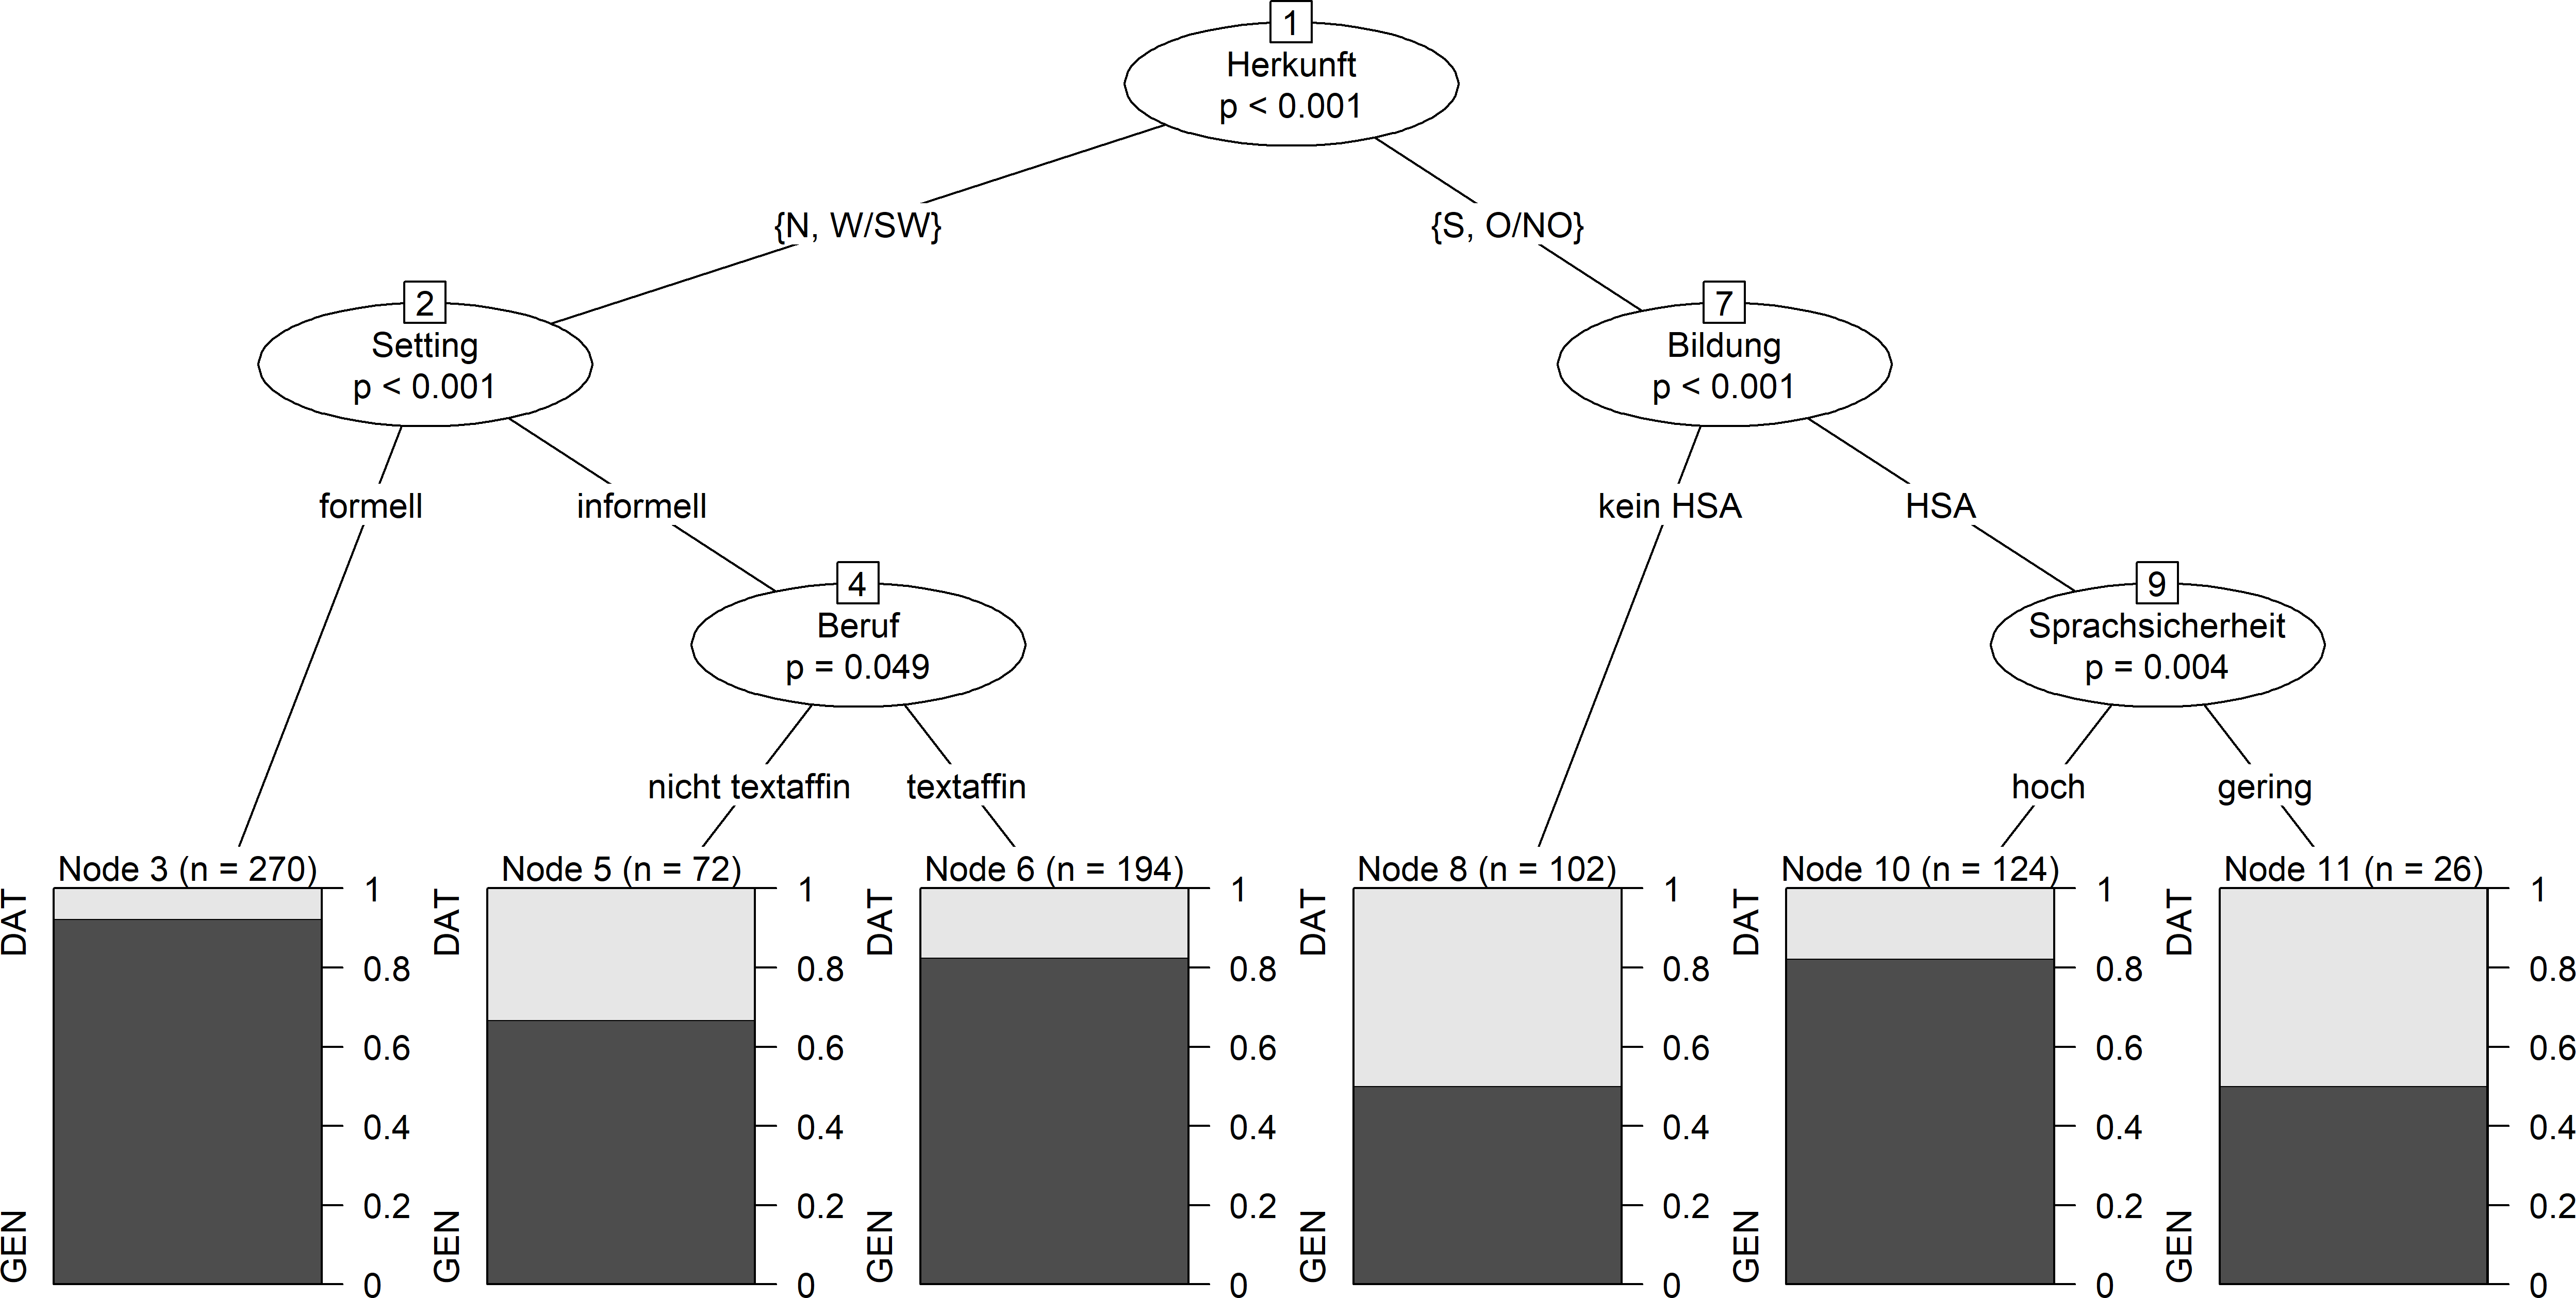
\includegraphics[angle=90, height=.9\textheight]{CtreeProdWegen.png}
\caption{\textit{Conditional Inference Tree} für die Kasuswahl bei \wegen}
\label{pic:CtreeProdWegen}
\end{figure}

Wie in \autoref{sec:ErgAkzCTrees} erläutert, berechnet das \textit{Random Forest}-Modell, wie groß der Einfluss der einzelnen Variablen auf die Kasuswahl ist:  
Je größer die \textit{Conditional Variable Importance} ist, desto größer ist der Einfluss der Variable \citep[s.][298--299]{Levshina.2015}. 
Für die Herkunft liegt die \textit{Conditional Variable Importance} bei 0,02. 
Sie ist damit der wichtigste Einflussfaktor für die Kasuswahl bei \wegen. 
Weitere relativ wichtige Faktoren sind die Bildung und das Setting (\textit{Conditional Variable Importance} jeweils bei 0,009). 
Alle anderen Faktoren weisen deutlich geringere Werte auf, scheinen die Kasuswahl bei \wegen{} also nicht nennenswert zu beeinflussen. 
Mithilfe des Pakets Hmisc \citep[][Version 4.4-0]{Harrell.2020} kann der C-Wert für einen \textit{Random Forest} ausgegeben werden, der ein Maß für die Passung des Modells ist \citep[s.][299]{Levshina.2015}. 
Der C-Wert für den \textit{Random Forest} zur Kasuswahl bei \wegen{} beträgt 0,88, demnach passt das Modell gut auf die Daten.  
%\begin{figure}
%\centering
%\includegraphics[width=\textwidth]{varimpProdwegen.png}
%\caption{Variable Importance für die Kasuswahl bei \wegen}
%\label{pic:varimpProdWegen}
%\end{figure}

Auch der \textit{Conditional Inference Tree} für die Kasuswahl bei \waehrend{} teilt die Daten zunächst anhand der regionalen Herkunft der Befragten (s. \autoref{pic:CtreeProdWaehrend}). 
Befragte aus Süddeutschland unterscheiden sich in ihrer Kasuswahl von Befragten aus Nord-, West- bzw. Südwest und Ost- bzw. Nordostdeutschland. 
In beiden Gruppen werden die Daten anhand des Settings weiter unterteilt. 
Bei Befragten aus süddeutschen Bundesländern im informellen Setting sagt das Modell die geringste Wahrscheinlichkeit für \waehrend{} plus Genitiv voraus.
Diese ist mit über 0,6 immer noch recht hoch. 
Im formellen Setting wird für süddeutsche Befragte mit ca. 0,9 jedoch eine deutlich höhere Wahrscheinlichkeit für den Genitiv angegeben. 

Bei Befragten aus nord-, west- bzw. südwest und ost- bzw. nordostdeutschen Bundesländern liegt die vorhergesagte Wahrscheinlichkeit für die Genitivrektion in allen Gruppen bei über 0,8. 
Das Setting wie auch die Reihenfolge, die im \textit{Tree} einen weiteren Split erzeugt, verändern die Wahrscheinlichkeiten hier nur geringfügig. 
Die \textit{Conditional Variable Importance} für die Herkunft und das Setting liegt jeweils bei 0,005. 
Für alle weiteren Faktoren sagt der \textit{Random Forest} eine \textit{Conditional Variable Importance} von oder bei null vorher. 
Diese haben also kaum einen Einfluss. 
Der C-Wert für den \textit{Random Forest} zu \waehrend{} liegt bei 0,9, das Modell repräsentiert die Daten also sehr gut. 
\begin{figure}
\centering
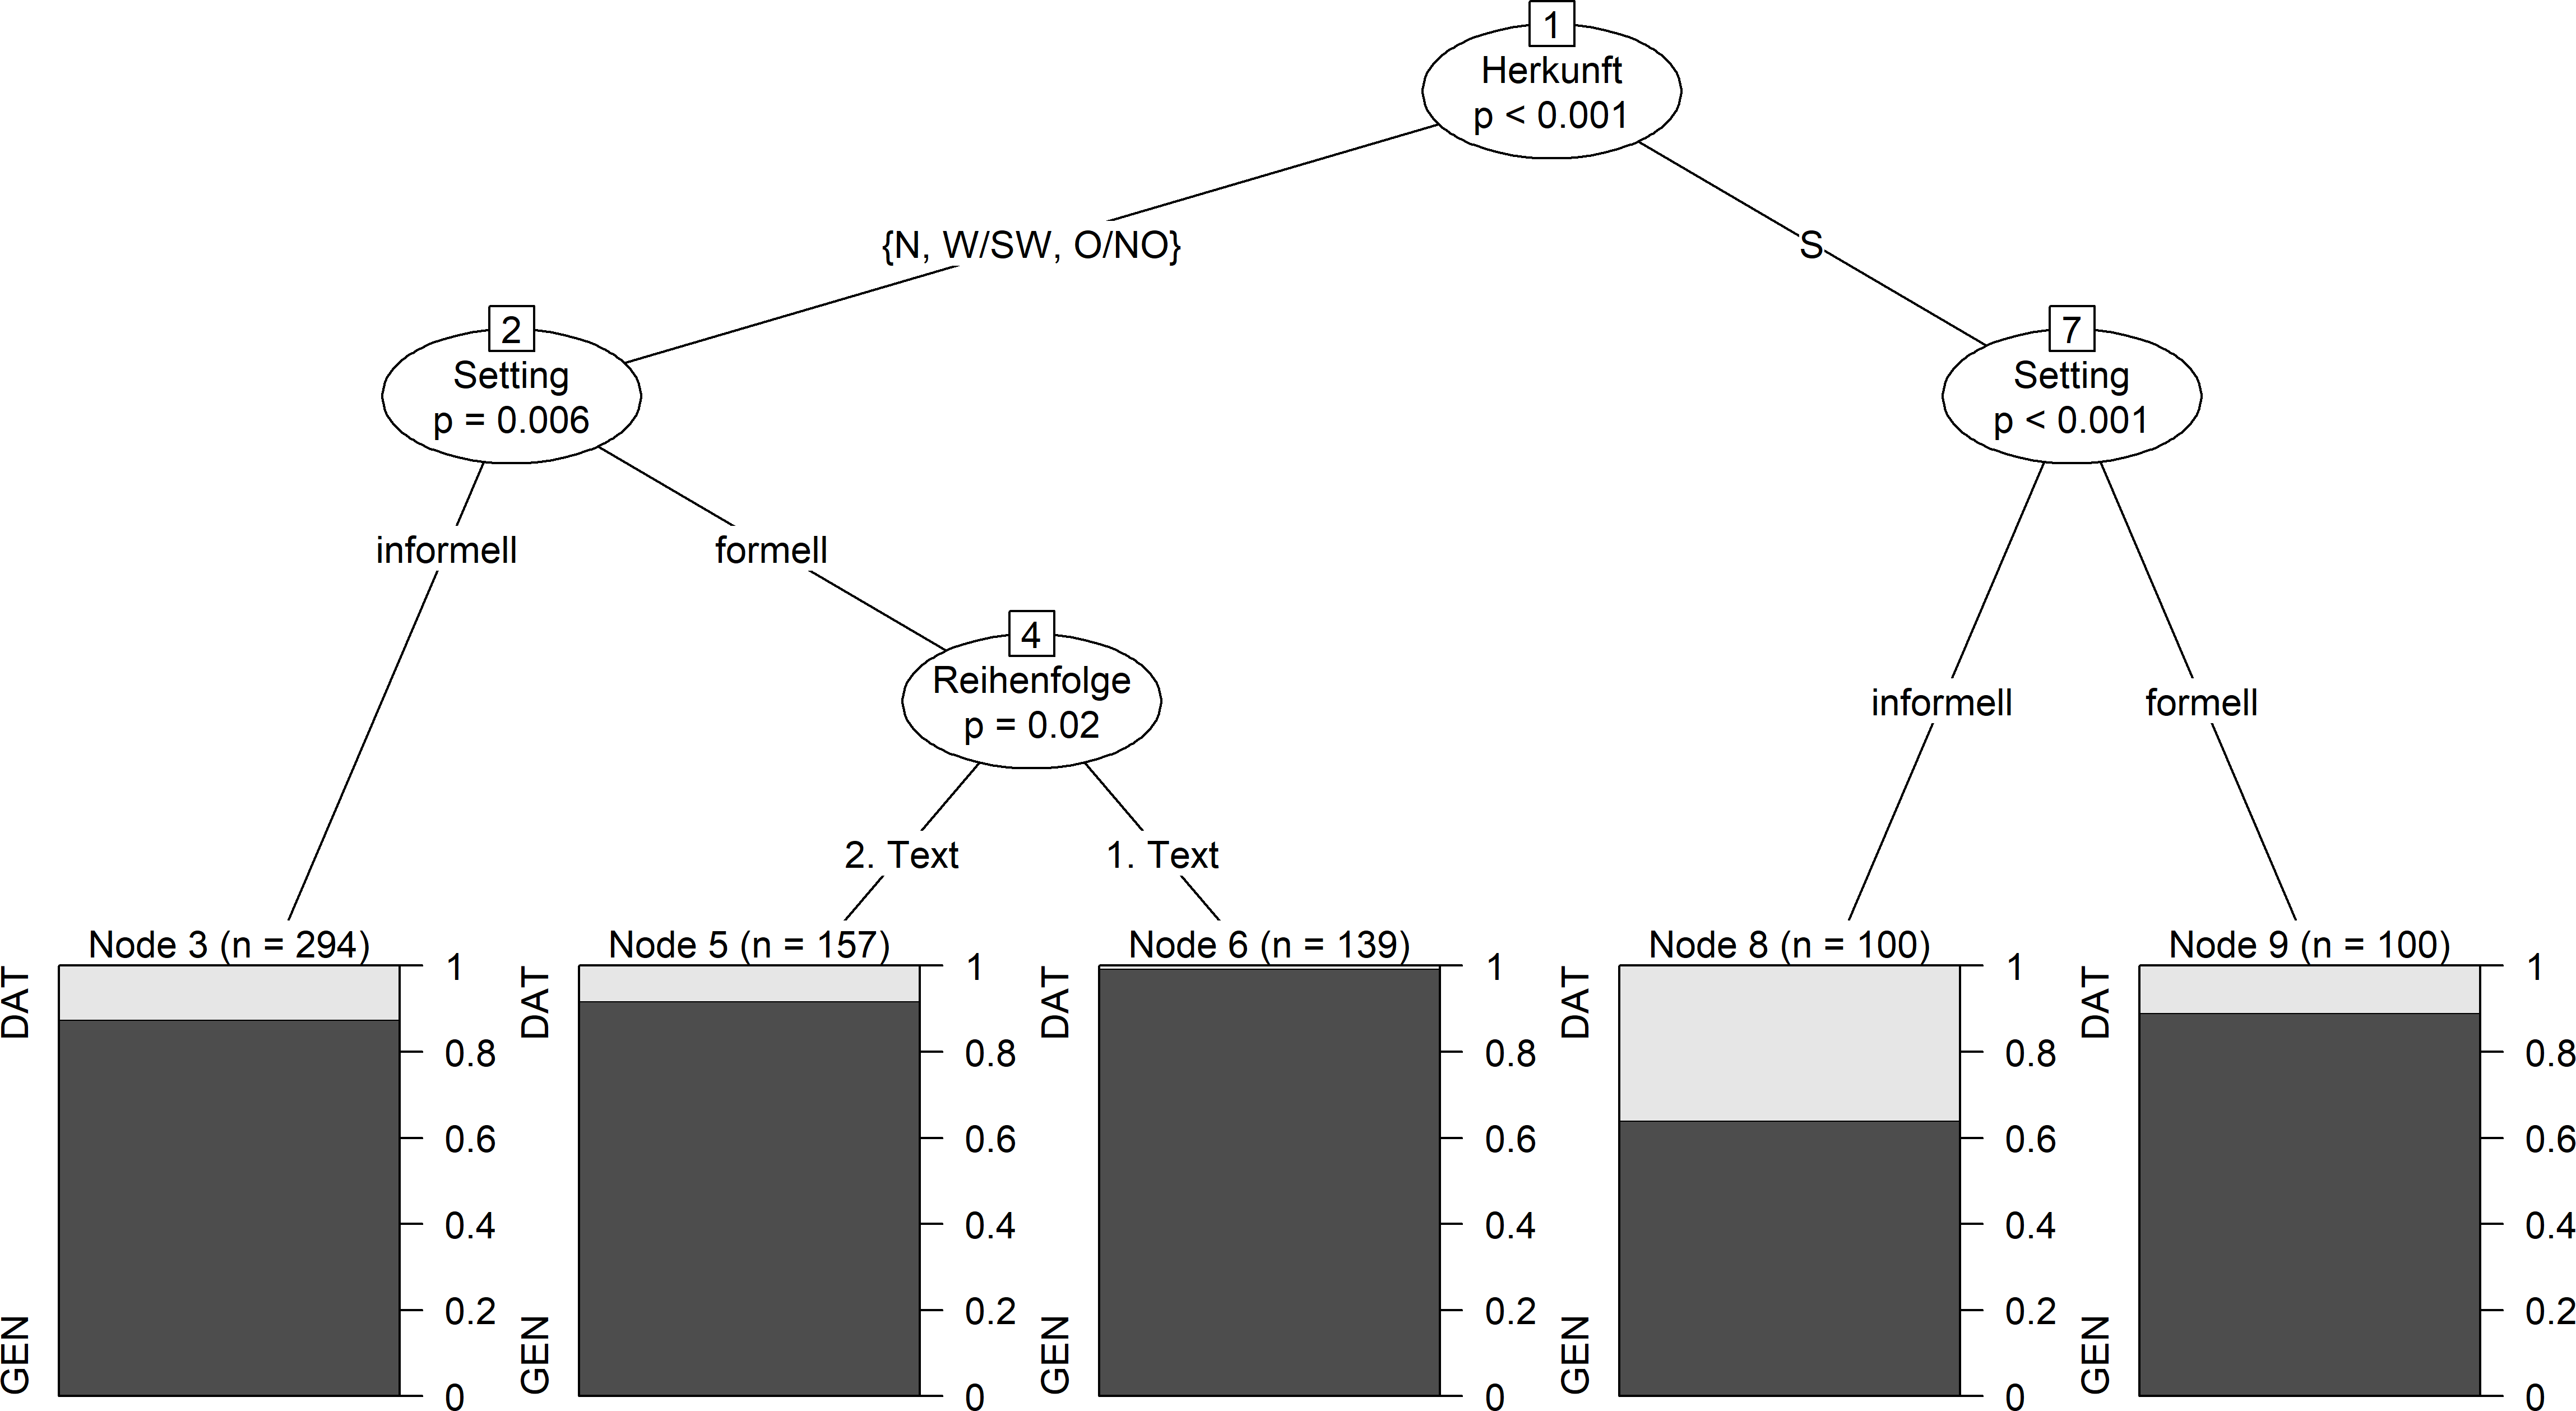
\includegraphics[angle=90, height=.9\textheight]{CtreeProdwaehrend.png}
\caption{\textit{Conditional Inference Tree} für die Kasuswahl bei \waehrend}
\label{pic:CtreeProdWaehrend}
\end{figure}
%
%\begin{figure}
%\centering
%\includegraphics[width=\textwidth]{varimpProdwaehrend.png}
%\caption{Variable Importance für die Kasuswahl bei \waehrend}
%\label{pic:varimpProdWaehrend}
%\end{figure}

\autoref{pic:CtreeProdDank} zeigt den \textit{Conditional Inference Tree} für die Kasuswahl bei \dank. 
Wie bereits bei \wegen{} und \waehrend{} wird der erste Split in den Daten nach der Herkunft der Befragten vorgenommen. 
Die insgesamt 589 Antworten von Befragten aus nord-, west- bzw. südwestdeutschen und ost- bzw. nordostdeutschen Bundeländern werden nicht weiter unterteilt. 
Hier gibt das Modell eine Wahrscheinlichkeit von über 0,9 für die Genitivrektion an. 
Bei Befragten aus Süddeutschland verzweigt sich der \textit{Tree} anhand der Formalität des Settings weiter.
Nur im formellen Lückentext liegt die Wahrscheinlichkeit für den Genitiv auf einem ähnlich hohen Niveau wie bei den Befragten, die nicht aus Süddeutschland stammen (s. \textit{Node} 7).
Die Antworten süddeutscher Befragter im informellen Lückentext werden noch einmal anhand des Bildungsstands der Befragten geteilt:
Bei süddeutschen Befragten ohne Hochschulabschluss ist die Wahl von Genitiv und Dativ ungefähr gleich wahrscheinlich. 
Dagegen gibt es bei süddeutschen Befragten mit Hochschulabschluss eine klare Tendenz zum Genitiv (Wahrscheinlichkeit ca. 0,8). 
Der \textit{Random Forest} gibt eine \textit{Variable Importance} von 0,004 für die Herkunft an und von 0,002 für das Setting und den Bildungsstand. 
Die Herkunft ist also auch hier der einflussreichste Faktor. 
Die Passung des \textit{Random Forests} für die Kasuswahl bei \dank{} ist mit einem C-Wert von 0,89 gut. 

Die \textit{Conditional Inference Trees} für \gegenueber{} und \object{seit} erzeugen keine Splits in den Daten (s. \autoref{pic:AnhCtreeProdGegenueber} und \autoref{pic:AnhCtreeProdSeit} im Anhang). 
Die von den \textit{Random Forests} zu diesen beiden Präpositionen berechneten \textit{Variable Importances} liegen für alle Faktoren bei oder nahe null.
Hier hat also keiner der Faktoren einen Einfluss darauf, ob Genitiv oder Dativ gewählt wird. 
Die Passungen sind für beide Modelle sehr gut, der C-Wert liegt jeweils bei 0,94. 
%\begin{figure}
%\centering
%\includegraphics[width=\textwidth]{varimpProdgegenueber.png}
%\caption{Variable Importance für die Kasuswahl bei \gegenueber}
%\label{pic:varimpProdgegenueber}
%\end{figure}
%
%\begin{figure}
%\centering
%\includegraphics[width=\textwidth]{varimpProdseit.png}
%\caption{Variable Importance für die Kasuswahl bei \object{seit}}
%\label{pic:varimpProdSeit}
%\end{figure}

Die statistische Analyse der Daten aus dem Produktionsexperiment zeigt, dass für die Kasuswahl bei den untersuchten Präpositionen vor allem die regionale Herkunft der Befragten und der im Lückentext evozierte Grad an Formalität entscheidend sind. 
\begin{figure}
\centering
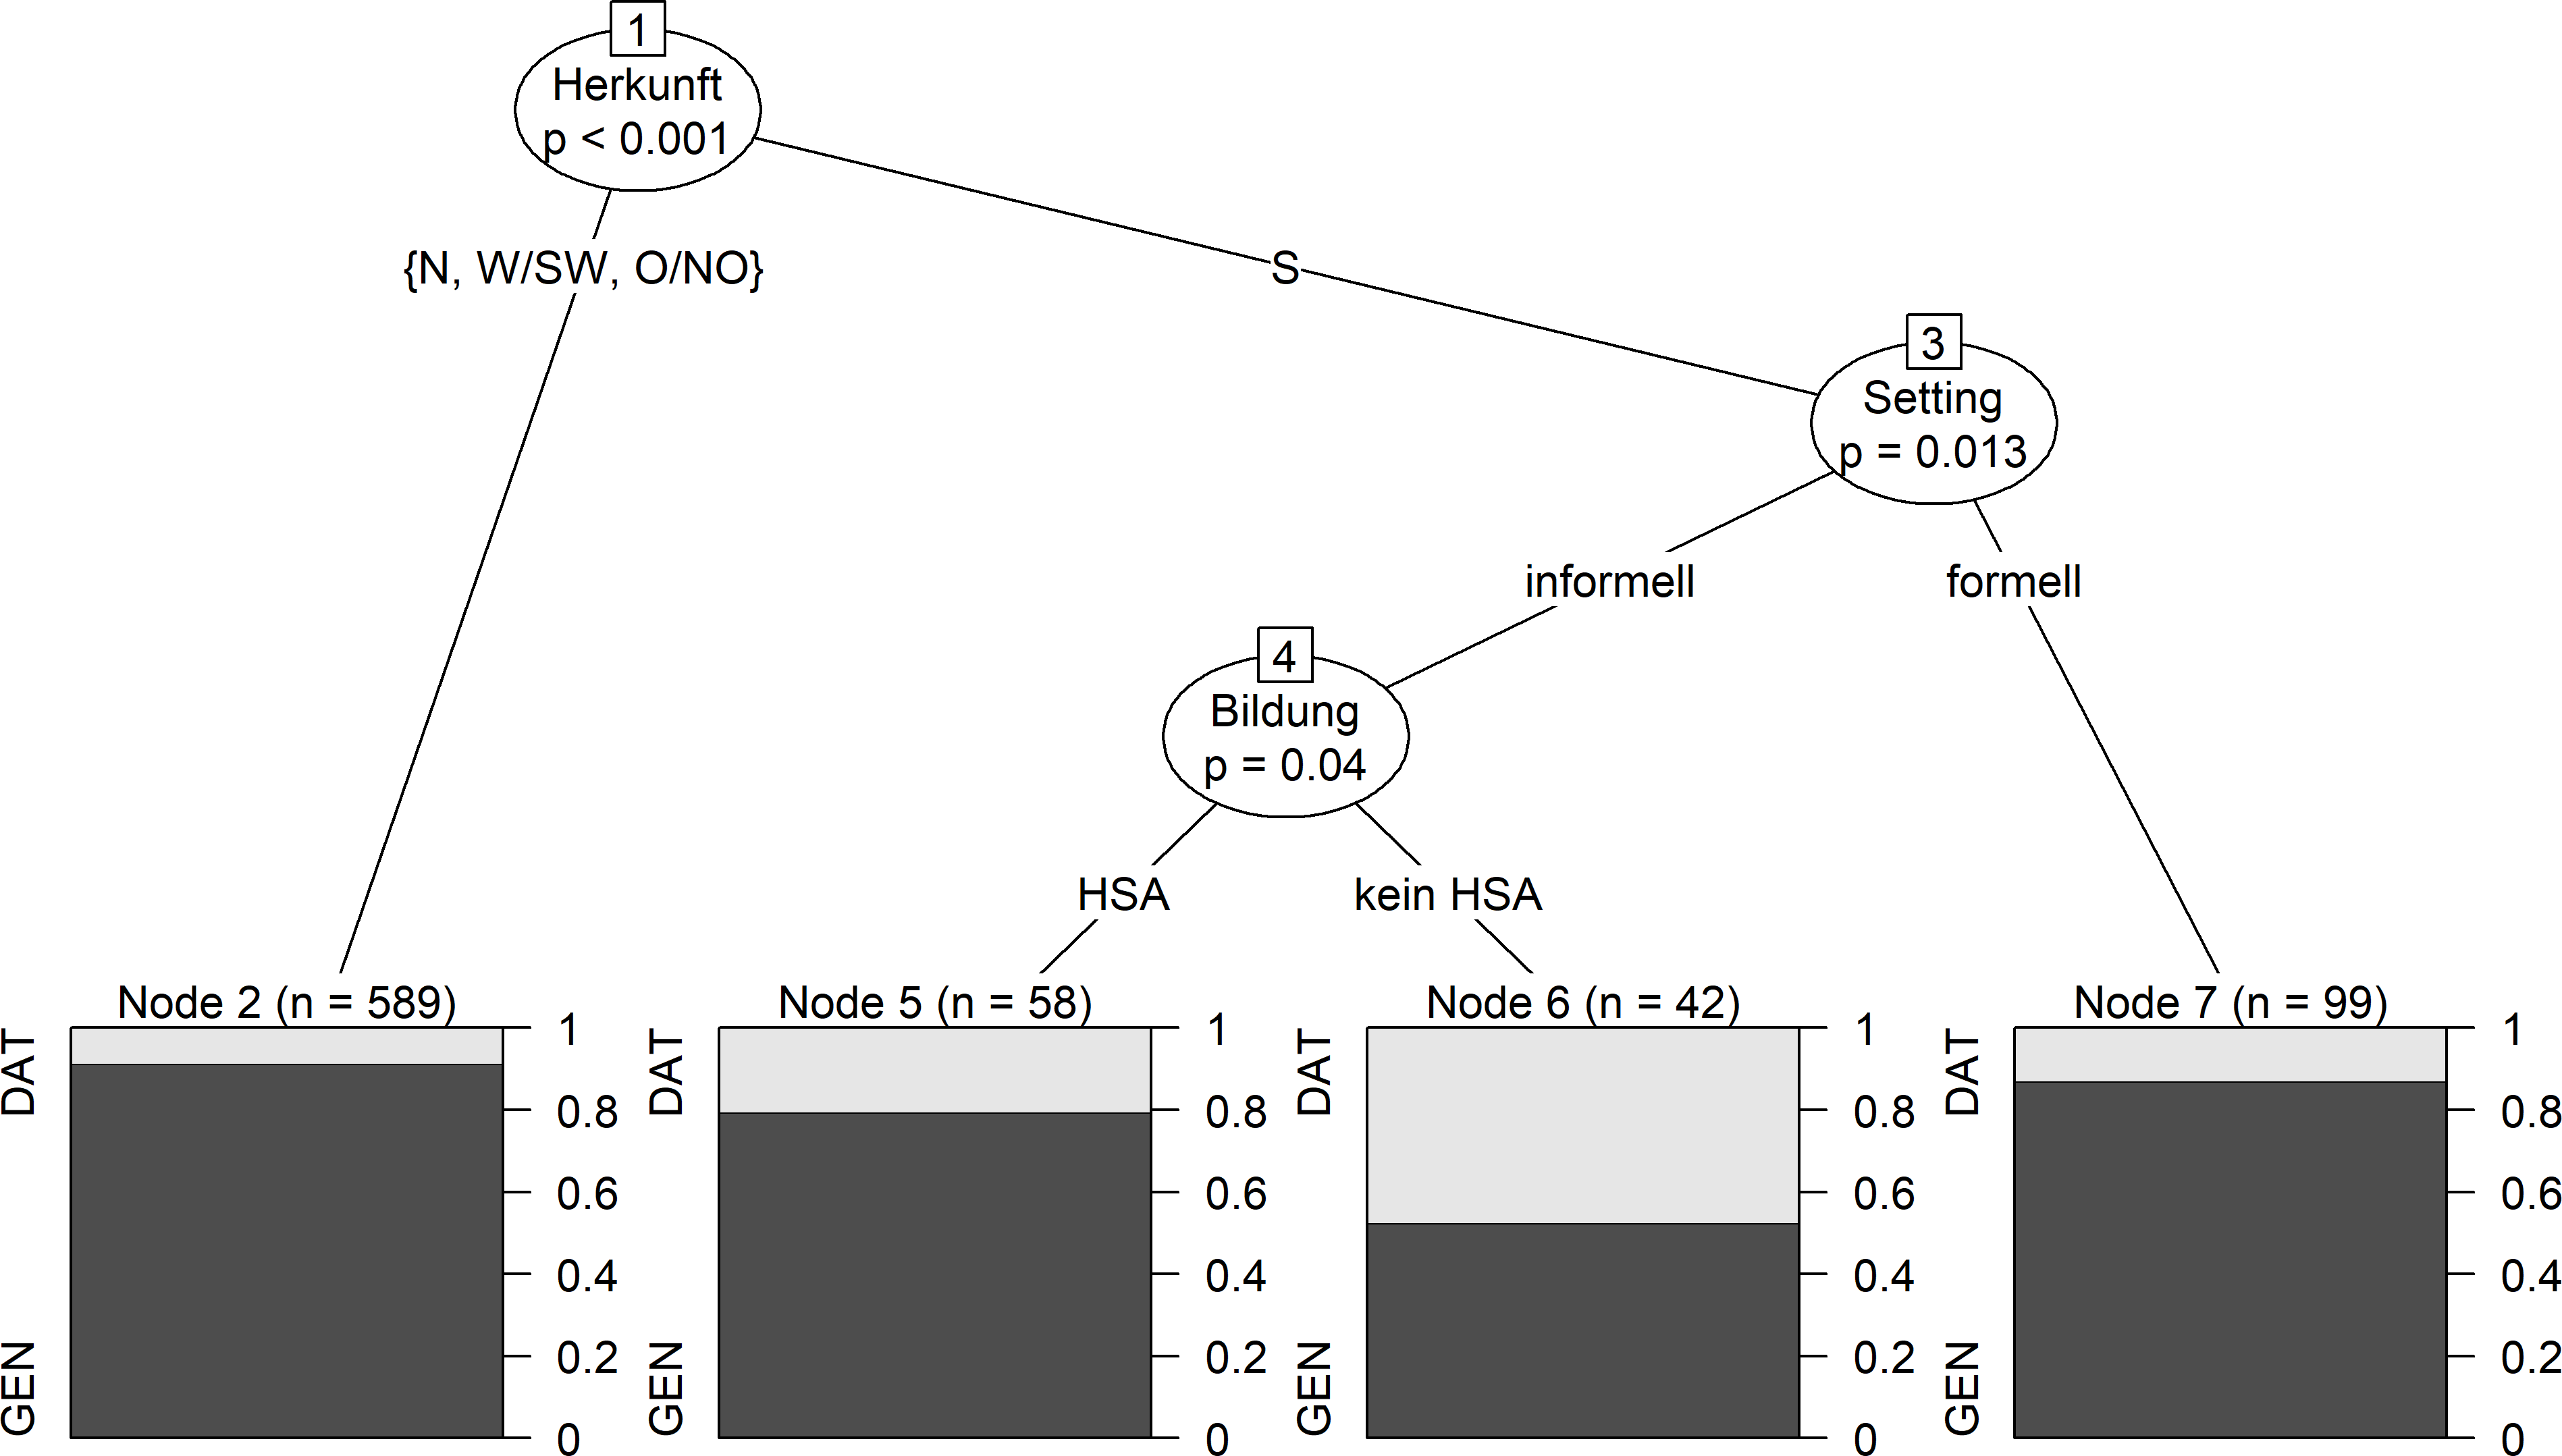
\includegraphics[angle=90, height=.9\textheight]{CtreeProddank.png}
\caption{\textit{Conditional Inference Tree} für die Kasuswahl bei \dank}
\label{pic:CtreeProdDank}
\end{figure}
%
%\begin{figure}
%\centering
%\includegraphics[width=\textwidth]{varimpProddank.png}
%\caption{Variable Importance für die Kasuswahl bei \dank}
%\label{pic:varimpProdDank}
%\end{figure}
%\subsection{Kasuswahl und Angaben im Akzeptabilitätstest}
%\label{sec:ErgProdNachAkz}
%Im Akzeptabilitätstest wurden die Befragten gebeten, die Korrektheit und die Angemessenheit der präsentierten Varianten zu bewerten und anzugeben, ob sie diese selbst verwenden würden. 
%Abgefragt wurden \wegen{} und \waehrend{} mit der Dativrektion sowie \dank{}, \gegenueber{} und die Primärpräposition \object{seit} mit der Genitivrektion.
%Im folgenden Abschnitt wird mithilfe von \textit{Random Forests} und \textit{Conditional Inference Trees} näher betrachtet, welche Zusammenhänge sich zwischen der Bewertung einer Variante im Akzeptabilitätstest und ihrer Verwendung im Produktionsexperiment erkennen lassen (für eine ausführliche Beschreibung von \textit{Random Forests} s. \autoref{sec:ErgAkzCTrees}). 
%Jede der fünf Varianten (\wegen{} und \waehrend{} plus Dativ sowie \dank{}, \gegenueber{} und \object{seit} plus Genitiv) wird zunächst im formellen und dann im informellen Setting betrachtet. 
%Die Ergebnisse des formellen Lückentexts werden mit den Antworten im formellen Teil des Akzeptabilitätstests abgeglichen, die Ergebnisse des informellen Lückentexts mit den Antworten im informellen Teil des Akzeptabilitätstests. 
%Für den Akzeptabilitätstest wurden die Befragten in vier Gruppen geteilt (\autoref{sec:Akz}). 
%Daher gehen in die Analyse zu einer Variante in einem Setting (etwa \wegen{} plus Dativ im formellen Setting) jeweils nur die Produktionsdaten derjenigen ein, die diese Präposition im Akzeptabilitätsteil im entsprechenden Setting bewertet haben. 
%Untersucht wird also bspw., wie die Akzeptabilitätswerte der 101 Befragten, die \wegen{} plus Dativ im formellen Setting bewerteten, mit der Kasuswahl derselben 101 Befragten im formellen Lückentext zusammenhängt. 
%
%Die abhängige Variable in den \textit{Random Forests} ist jeweils die Verwendung oder Nicht-Verwendung der Variante. 
%Die unabhängigen Variablen sind die Bewertung der Korrektheit und der Angemessenheit der Variante sowie die Angaben der Befragten, ob sie die Variante selbst verwenden würden. 
%\autoref{table:CtreesVariablenProdAkz} gibt einen Überblick über die Variablen, deren Einfluss überprüft wird, und ihre Ausprägungen.\footnote{Die \textit{Random Forests} und die \textit{Conditional Inference Trees} wurden mit dem Paket \glqq party\grqq{} \citep{Hothorn.2010} gerechnet. Folgender Code wurde in R verwendet (hier beispielhaft die Codes für \wegen{} plus Dativ im formellen Setting: \\
%\textit{Conditional Inference Tree}: ProdAkzWegenDatFormell.ctree = ctree(Prod \~{} Bewertung\_Korrektheit + Bewertung\_Angemessenheit + eigene\_Verwendung, controls = ctree\_control(minbucket=10), data = ProdAkzWegenDatFormell)\\
%\textit{Random Forest}: data.controls <- cforest_unbiased(ntree=1000, mtry=2)\\
%forestProdAkzWegenDatFormell <- cforest(Prod \~{} Bewertung\_Korrektheit + Bewertung\_Angemessenheit + eigene\_Verwendung, ProdAkzWegenDatFormell, controls = data.controls)}
%\begin{table}
%\centering
%\begin{tabular}{ll}
%\textbf{Variable}  & \textbf{Ausprägungen}                                                                                   \\ \hline
%Bewertung Korrektheit           & korrekt, inkorrekt
%\\ \hline
%Bewertung Angemessenheit              & angemessen, unangemessen
%\\ \hline
%eigene Verwendung           & ja, nein
%\\ 
%\end{tabular}
%\caption{Variablen des Akzeptabilitätstests als Einflussfaktoren auf die Kasuswahl im Produktinsexperiment}
%\label{table:CtreesVariablenProdAkz}
%\end{table}
%
%\autoref{pic:CtreeProdAkzWegenDatFormell} zeigt den \textit{Conditional Inference Tree} für den Einfluss der Akzeptabilitätswerte von \wegen{} plus Dativ im formellen Setting auf die Verwendung der Variante im formellen Lückentext. 
%Die Daten werden nur anhand der Bewertung der Korrektheit gesplittet. 
%Für die 14 Befragten, die die Dativrektion bei \wegen{} im formellen Setting als korrekt bewerten, liegt die Wahrscheinlichkeit, dass sie diese Variante im formellen Lückentext gebrauchen bei 0,5.
%Dagegen beträgt die Wahrscheinlichkeit, \wegen{} plus Dativ im formellen Lückentext zu verwenden, für die Befragten, die die Variante im formellen Setting als inkorrekt bewerten, weniger als 0,2. 
%Wie Befragte die Korrektheit des Dativs bewerten, hat hier also den größten Einfluss darauf, ob sie ihn im Produktionsexperiment selbst verwenden. 
%Das zeigt auch die vom \textit{Random Forest} ausgegebene \textit{Variable Importance}: Für die Bewertung der Korrektheit liegt sie bei 0,028, für die Angaben zur eigenen Verwendung hingegen nur bei 0,01 und für die Bewertung der Angemessenheit bei 0. 
%Mit dem Paket \glqq Hmisc\grqq{} \cite{Harrell.2020}  wurde der C-Wert berechnet, der ein Maß dafür ist, wie gut das Modell die Daten repräsentiert. 
%Mit 0,77 liegt die Passung im mittleren Bereich. 
%\begin{figure}
%\centering
%\includegraphics[width=\textwidth]{CtreeProdAKzWegenDatFormell.png}
%\caption{Conditional Inference Tree für die Verwendung von \wegen{} plus Dativ im formellen Lückentext}
%\label{pic:CtreeProdAkzWegenDatFormell}
%\end{figure}
%
%Der \textit{Conditional Inference Tree} für die Dativrektion bei \wegen{} im informellen Setting teilt die Daten anhand der Angaben zur eigenen Verwendung (s. \autoref{pic:CtreeProdAkzWaehrendDatInformell}):
%Für Befragte, die im Akzeptabilitätstest zustimmen, dass sie \wegen{} plus Dativ in einem Gespräch unter Freunden (informelles Setting) verwenden würden, sagt das Modell die Dativrektion mit einer Wahrscheinlichkeit von 0,6 voraus. 
%Bei Befragten, die angeben, \wegen{} plus Dativ hier nicht zu verwenden, liegt die Wahrscheinlichkeit hingegen bei unter 0,2. 
%Wie sich an der \textit{Variable Importance} ablesen lässt, spielt die Bewertung der Korrektheit (0,069) im Vergleich zu den Angaben zur eigenen Verwendung (0,102) eine untergeordnete Rolle. 
%Die Bewertung der Angemessenheit hat keinen Einfluss (\textit{Variable Importance} = 0). 
%Das Modell passt mit einem C-Wert von 0,81 gut auf die Daten. 
%\begin{figure}
%\centering
%\includegraphics[width=\textwidth]{CtreeProdAKzWegenDatInformell.png}
%\caption{Conditional Inference Tree für die Verwendung von \wegen{} plus Dativ im informellen Lückentext}
%\label{pic:CtreeProdAkzWegenDatInformell}
%\end{figure}
%
%Bei der Verwendung der Dativrektion bei \waehrend{} im formellen Lückentext kann kein systematischer Zusammenhang mit einer der Variablen aus dem Akzeptabilitätstest festgestellt werden: 
%Der \textit{Conditional Inference Tree} erzeugt keinen Split in den Daten und alle \textit{Variable Importances} betragen null. 
%Die Passung des \textit{Random Forests} liegt bei 0,73. 
%
%
%\begin{figure}
%\centering
%\includegraphics[width=\textwidth]{CtreeProdAkzWaehrendDatInformell.png}
%\caption{Conditional Inference Tree für die Verwendung von \waehrend{} plus Dativ im informellen Lückentext}
%\label{pic:CtreeProdAkzWaehrendDatInformell}
%\end{figure}
%
%\begin{figure}
%\centering
%\includegraphics[width=\textwidth]{CtreeProdAkzDankGenformell.png}
%\caption{Conditional Inference Tree für die Verwendung von \dank{} plus Genitiv im formellen Lückentext}
%\label{pic:CtreeProdAkzDankGenFormell}
%\end{figure}
%
%\begin{figure}
%\centering
%\includegraphics[width=\textwidth]{CtreeProdAkzDankGeninformell.png}
%\caption{Conditional Inference Tree für die Verwendung von \dank{} plus Genitiv im informellen Lückentext}
%\label{pic:CtreeProdAkzDankGenInformell}
%\end{figure}
%
%\begin{figure}
%\centering
%\includegraphics[width=\textwidth]{CtreeProdAkzGegenueberGenformell.png}
%\caption{Conditional Inference Tree für die Verwendung von \gegenueber{} plus Genitiv im formellen Lückentext}
%\label{pic:CtreeProdAkzGegenueberGenFormell}
%\end{figure}
%
%gegenueber informell: kein Split
%
%\begin{figure}
%\centering
%\includegraphics[width=\textwidth]{CtreeProdAkzSeitGenformell.png}
%\caption{Conditional Inference Tree für die Verwendung von \object{seit} plus Genitiv im formellen Lückentext}
%\label{pic:CtreeProdAkzSeitGenFormell}
%\end{figure}
%
%\begin{figure}
%\centering
%\includegraphics[width=\textwidth]{CtreeProdAkzSeitGeninformell.png}
%\caption{Conditional Inference Tree für die Verwendung von \object{seit} plus Genitiv im informellen Lückentext}
%\label{pic:CtreeProdAkzSeitGenInformell}
%\end{figure}
%
%%
%%\autoref{pic:ErgProdWegenNachAkz} zeigt die Zusammenhänge zwischen der Kasuswahl bei \wegen{} im formellen und im informellen Lückentext mit der Akzeptabilität von \wegen{} plus Dativ im formellen und im informellen Setting.
%%Zu sehen ist, das von den Befragten, die die Dativrektion bei \wegen{} als korrekt erachten jeweils deutlich mehr diese Variante auch im Lückentext verwenden. 
%%Allerdings wählen in beiden Lückentexten auch Befragte die Dativrektion, die im Akzeptabilitätstest angeben, diese sei inkorrekt. 
%%Von den 70 Befragten, die \wegen{} plus Dativ in einem informellen Gespräch für inkorrekt halten, verwenden 17 diese Variante im informellen Lückentext. 
%%Auch unter den Befragten, die die Dativrektion als unangemessen einstufen, sind im formellen und im informellen Setting einzelne, die die Variante im Lückentext dennoch verwenden. 
%%\begin{figure}
%%\centering
%%\includegraphics[width=\textwidth]{ProdWegenNachAkz.jpg}
%%\caption{Zusammenhang der Kasuswahl bei \wegen{} mit der Akzeptabilität von \wegen{} plus Dativ}
%%\label{pic:ErgProdWegenNachAkz}
%%\end{figure}
%%
%%\begin{figure}
%%\centering
%%\includegraphics[width=\textwidth]{ProdwaehrendNachAkz.jpg}
%%\caption{Zusammenhang der Kasuswahl bei \waehrend{} mit der Akzeptabilität von \waehrend{} plus Dativ}
%%\label{pic:ErgProdWaehrendNachAkz}
%%\end{figure}
%%
%%\begin{figure}
%%\centering
%%\includegraphics[width=\textwidth]{ProddankNachAkz.jpg}
%%\caption{Zusammenhang der Kasuswahl bei \dank{} mit der Akzeptabilität von \dank{} plus Genitiv}
%%\label{pic:ErgProdDankNachAkz}
%%\end{figure}
%%
%%\begin{figure}
%%\centering
%%\includegraphics[width=\textwidth]{ProdgegenueberNachAkz.jpg}
%%\caption{Zusammenhang der Kasuswahl bei \gegenueber{} mit der Akzeptabilität von \gegenueber{} plus Genitiv}
%%\label{pic:ErgProdGegenueberNachAkz}
%%\end{figure}
%%
%%\begin{figure}
%%\centering
%%\includegraphics[width=\textwidth]{ProdseitNachAkz.jpg}
%%\caption{Zusammenhang der Kasuswahl bei \object{seit} mit der Akzeptabilität von \object{seit} plus Genitiv}
%%\label{pic:ErgProdSeitNachAkz}
%%\end{figure}

\subsection{Zusammenfassung der Auswertung des Produktionsexperiments}
\label{sec:ErgProdZusammenfassung}
Im Produktionsexperiment wurden Befragte gebeten, einen formellen und einen informellen Lückentext mit vorgegebenen Substantiven zu vervollständigen. 
Diese sollten in der entsprechenden Form zusammen mit einem Definitartikel in Lücken nach den Präpositionen \wegen, \waehrend, \dank, \gegenueber{} und \object{seit} eingetragen werden. 
In den Produktionsdaten zeigt sich eine generelle Tendenz zur Genitivrektion bei den Präpositionen \wegen, \waehrend{} und \dank{}. 
\object{Gegenüber} und \object{seit} hingegen werden in den allermeisten Fällen mit dem Dativ gebraucht. 
Obwohl bei \wegen, \waehrend{} und \dank{} der Genitiv im formellen und im informellen Text überwiegt, gibt es recht große Unterschiede zwischen den Settings: 
Im informellen Lückentext wird der Dativ deutlich häufiger gesetzt als im formellen. 
Die statistische Überprüfung mithilfe von \textit{Random Forests} ergibt, dass das Setting die Kasuswahl systematisch beeinflusst. 
Die Ergebnisse des Produktionsexperiments deuten damit darauf hin, dass die Indexikalität der Rektionsvarianten wesentlich für ihre Verwendung ist. 
Die Befragten nutzen die Indexikalität der Rektionsvarianten, um verschiedene Formalitätsgrade anzuzeigen. 

Ein weiterer systematischer Einflussfaktor neben dem Setting ist die regionale Herkunft der Befragten: 
Die Genitivrektion wird von norddeutschen Befragten häufiger verwendet, die Dativrektion von süddeutschen. 
Für die anderen besprochenen Faktoren (Alter, Bildungsstand, Textaffinität des Berufs, Einschätzung der eigenen Sprachsicherheit und Variationstoleranz) lassen sich in den \textit{Random Forests} keine systematischen Effekte auf die Verteilung der Kasusrektion erkennen. 
In der detaillierten Betrachtung der Ergebnisse in \autoref{sec:ErgProdNachAlter} bis \autoref{sec:ErgProdNachVT} treten dennoch einige Unterschiede zwischen den jeweiligen Gruppen hervor. 
So wird deutlich, dass ältere Befragte bei \dank{} nicht die ältere Variante (\dank{} plus Dativ) häufiger gebrauchen, sondern die Genitivrektion, die in der Wahrnehmung der Befragten die ältere Variante darstellt (\autoref{sec:ErgAssSprachwandel}). 
Zudem zeigen sich Unterschiede in der Kontextsensitivität der Gruppen. 
Bspw. differenzieren Befragte aus textaffinen Berufen bei ihrer Kasuswahl weniger stark zwischen dem formellen und dem informellen Lückentext als Befragte aus nicht-textaffinen Berufen.
Ebenso variieren variationstolerante Befragte stärker zwischen den Settings als weniger variationstolerante. 

Im folgenden Kapitel werden die Ergebnisse des Assoziationsteils, des Akzeptabilitätsteils und des Produktionsteils aus dem Fragebogen zur Kasusrektion von \wegen, \waehrend{}, \dank, \gegenueber{} und \object{seit} diskutiert und zueinander in Beziehung gesetzt. 

%\section{Positionierungen einzelner Befragter}
%\label{sec:ErgPositionierung}



